\documentclass[11pt]{article}
\setlength{\columnsep}{1.5cm}
\usepackage[left=1.5cm,right=1.5cm,top=2.5cm,bottom=2.5cm,columnsep=1.5cm]{geometry}

% Define a command for technical term explanations
\usepackage{amsthm}
\usepackage{tcolorbox}
\usepackage{xcolor}
\usepackage{amsmath}
\newtheorem{definition}{Definition}
\newenvironment{termbox}[1]
  {\begin{tcolorbox}[colback=blue!5!white,colframe=blue!75!black,title=#1,fonttitle=\bfseries]}
  {\end{tcolorbox}}
\usepackage{graphicx}
\usepackage{subcaption}
\usepackage{booktabs}
\usepackage{adjustbox}
\usepackage{tabularx}
\usepackage{multirow}
\usepackage{algorithm}
\usepackage{algpseudocode}
\usepackage[T1]{fontenc}
\usepackage{setspace}
\setstretch{1.05}
% Prevent redefinition of algorithmic commands
\providecommand{\algorithmicindent}{0em}
\usepackage{enumitem}
\usepackage{wrapfig}
\usepackage{cite}
\usepackage{amssymb,amsfonts}
\usepackage{textcomp}
\usepackage{listings}
\usepackage{hyperref}
\usepackage{float}
\usepackage{tikz}
\usetikzlibrary{shadows,arrows,shapes,positioning}
% Define fill opacity=0.9 style for TikZ
\tikzset{
  fill opacity=0.9/.style={
    general shadow={shadow xshift=0.7ex, shadow yshift=-0.7ex, opacity=0.4, fill=black!50, every shadow}
  }
}
\tikzset{every shadow/.style={}}
\usepackage{pgfplots}
\pgfplotsset{compat=1.18}
\usepackage{multicol}

% Add the newunicodechar package to handle Unicode characters
\usepackage{newunicodechar}


% Define Unicode chess pieces with proper spacing


% For multiplication symbol

% Fix algorithm package conflicts
\renewcommand{\algorithmicrequire}{\textbf{Input:}}
\renewcommand{\algorithmicensure}{\textbf{Output:}}

% Define colors for code listings
\definecolor{codegreen}{rgb}{0,0.6,0}
\definecolor{codegray}{rgb}{0.5,0.5,0.5}
\definecolor{codepurple}{rgb}{0.58,0,0.82}
\definecolor{backcolour}{rgb}{0.95,0.95,0.92}

% Configure code listings
\lstset{
    backgroundcolor=\color{backcolour},
    commentstyle=\color{codegreen},
    keywordstyle=\color{magenta},
    numberstyle=\tiny\color{codegray},
    stringstyle=\color{codepurple},
    basicstyle=\ttfamily\footnotesize,
    breakatwhitespace=false,
    breaklines=true,
    captionpos=b,
    keepspaces=true,
    numbers=left,
    numbersep=5pt,
    showspaces=false,
    showstringspaces=false,
    showtabs=false,
    tabsize=2
}

% Define Python style for listings
\lstdefinestyle{Python}{
    language=Python,
    morekeywords={self, if, else, return, try, except, raise, finally, import, from, as, def, class, for, while, with, True, False, None, and, or, not, in, is, lambda, yield, break, continue, pass, assert, del, global, nonlocal}
}

% Add spacing between sections
\usepackage{titlesec}
\titlespacing*{\section}{0pt}{3.5ex plus 1ex minus .2ex}{2.3ex plus .2ex}
\titlespacing*{\subsection}{0pt}{3.25ex plus 1ex minus .2ex}{1.5ex plus .2ex}

% Add spacing between items in lists
\setlist[itemize]{itemsep=0.2em, parsep=0.2em}
\setlist[enumerate]{itemsep=0.2em, parsep=0.2em}

% Add spacing between paragraphs
\setlength{\parskip}{0.5em}

% Add spacing between figures
\setlength{\floatsep}{1em}
\setlength{\textfloatsep}{1em}
\setlength{\intextsep}{1em}

\begin{document}

\title{Understanding Chess AI: From Simple Algorithms to Deep Reinforcement Learning\\\large A Beginner's Guide to Multi-Agent Deep Reinforcement Learning for Chess}
\author{Chess AI Research Team}
\date{}

\maketitle

\begin{abstract}
This document explains how computers play chess, starting from the simplest methods to advanced artificial intelligence. Written for beginners (even 10-year-olds can understand it!), we explore how chess-playing AI has evolved over time. We start with basic algorithms like Minimax, then move to more complex approaches like Monte Carlo Tree Search, and finally dive into modern deep reinforcement learning techniques. The document focuses on a specific project called Simple-MADRL-Chess, which uses multiple AI agents that learn by playing against each other. We explain every part of the code, how the neural networks work, and how the training process helps the AI get better at chess over time. Complete with examples, pictures, and step-by-step explanations, this guide makes complex AI concepts easy to understand.
\end{abstract}

\begin{center}
\textbf{Keywords:} Chess, Artificial Intelligence, Reinforcement Learning, Neural Networks, Minimax, Monte Carlo Tree Search, Multi-Agent Learning
\end{center}

\section{Introduction}
\subsection{What is Chess AI?}

Have you ever wondered how computers play chess? How do they know which moves to make? Can they really think like humans? In this document, we're going to explore the exciting world of chess-playing artificial intelligence (AI) in a way that anyone can understand - even if you're just 10 years old!

% --- Chessboard: Make it full-width and ensure rendering ---
\onecolumn

\begin{figure}[!htbp]
    \centering
    \newchessgame
    \setboardfontsize{28pt}
    \setchessboard{showmover=false, labelbottom=true, labelleft=true, boardfontfamily=lmss}
    \chessboard[setfen=rnbqkbnr/pppppppp/8/8/8/8/PPPPPPPP/RNBQKBNR]
    \caption{A chess board with pieces in starting position}
    \label{fig:chess_board}
\end{figure}

\twocolumn

Let's start with the basics of a chess board:
\begin{itemize}
    \item A chess board has 8 rows (called ranks) and 8 columns (called files)
    \item Each square is either light or dark
    \item There are 32 pieces total - 16 for each player
    \item Each type of piece moves differently
\end{itemize}

Chess AI is a computer program that can play chess by itself. It can analyze the board, think about possible moves, and choose what it believes is the best move. But computers don't "think" like we do. They follow instructions (called algorithms) that humans write for them. Over time, these algorithms have become more and more sophisticated, allowing computers to play chess at levels that can beat even the best human players in the world.

\subsection{Why Learn About Chess AI?}

Chess is a perfect game for teaching computers how to "think" because:
\begin{itemize}
    \item It has clear rules that don't change
    \item It requires planning and strategy
    \item You can measure how well you're doing (by winning or losing)
    \item It's complex enough to be interesting but simple enough to program
\end{itemize}

By understanding how chess AI works, you'll learn about many important concepts in computer science and artificial intelligence. These same ideas are used in self-driving cars, robots, game-playing systems, and many other exciting technologies!

\subsection{Our Journey Through Chess AI}

In this document, we'll take you on a journey through the evolution of chess AI:

\begin{enumerate}
    \item \textbf{Minimax Algorithm}

Let's start with the simplest way computers can play chess - the Minimax algorithm. Imagine you're playing a game of tic-tac-toe. You want to make the best move, but you also want to prevent your opponent from winning. That's exactly what Minimax does!

\begin{figure}[ht]
    \centering
    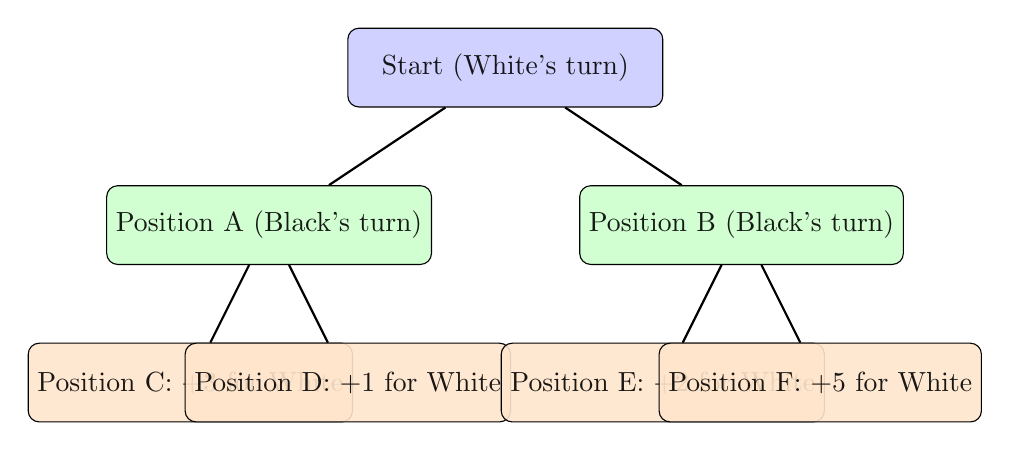
\begin{tikzpicture}[
        scale=1.0,
        transform shape,
        level distance=2cm,
        sibling distance=3cm,
        every node/.style={draw, rectangle, rounded corners, minimum width=4cm, minimum height=1cm, align=center, fill opacity=0.9}
    ]
        % Root node
        \node[fill=blue!20] (root) at (0,0) {Start (White's turn)};
        
        % Level 1 nodes
        \node[fill=green!20] (A) at (-3,-2) {Position A (Black's turn)};
        \node[fill=green!20] (B) at (3,-2) {Position B (Black's turn)};
        
        % Level 2 nodes
        \node[fill=orange!20] (C) at (-4,-4) {Position C: +3 for White};
        \node[fill=orange!20] (D) at (-2,-4) {Position D: +1 for White};
        \node[fill=orange!20] (E) at (2,-4) {Position E: +2 for White};
        \node[fill=orange!20] (F) at (4,-4) {Position F: +5 for White};
        
        % Connect nodes
        \draw[thick] (root) -- (A);
        \draw[thick] (root) -- (B);
        \draw[thick] (A) -- (C);
        \draw[thick] (A) -- (D);
        \draw[thick] (B) -- (E);
        \draw[thick] (B) -- (F);
    \end{tikzpicture}
    \caption{Minimax decision tree with improved spacing}
    \label{fig:minimax_tree}
\end{figure}

Here's how Minimax works:
\begin{enumerate}
    \item Look at all possible moves
    \item For each move, look at what your opponent could do
    \item For each of their moves, look at what you could do next
    \item Keep going until you reach the end of the game
    \item Choose the move that gives you the best outcome
\end{enumerate}, like Monte Carlo Tree Search.

    \item \textbf{Machine Learning}: Next, we'll see how computers can learn from experience instead of just following fixed rules.

    \item \textbf{Deep Reinforcement Learning}: Finally, we'll dive into modern AI techniques where computers teach themselves to play better by practicing millions of games.
\end{enumerate}

\subsection{The Simple-MADRL-Chess Project}

The main focus of this document is a special chess AI project called "Simple-MADRL-Chess." MADRL stands for "Multi-Agent Deep Reinforcement Learning." That's a fancy way of saying we have multiple AI players (agents) that learn by playing against each other and getting better over time.

We'll explain every part of this project in detail:
\begin{itemize}
    \item How the chess game is represented in the computer
    \item How the AI agents make decisions
    \item How they learn from their experiences
    \item How we train them to get better and better
\end{itemize}

By the end of this document, you'll understand how modern chess AI works, and you might even be inspired to create your own AI for chess or other games!

\section{The Basics of Chess AI}

\subsection{How Computers See Chess}

Before we dive into algorithms, let's understand how computers "see" a chess game. Unlike humans who look at the board and visually recognize pieces, computers need a way to represent the game mathematically.

\subsubsection{Board Representation}

The most common way to represent a chess board in a computer is using a grid of numbers, where each number represents a different piece. For example:
\begin{itemize}
    \item 0 might represent an empty square
    \item 1 might represent a white pawn
    \item 2 might represent a white knight
    \item And so on...
\end{itemize}

Here's a simple example of how a computer might see the starting position of a chess board:

\begin{center}
\begin{tabular}{|c|c|c|c|c|c|c|c|}
\hline
-3 & -2 & -3 & -5 & -6 & -3 & -2 & -3 \\
\hline
-1 & -1 & -1 & -1 & -1 & -1 & -1 & -1 \\
\hline
0 & 0 & 0 & 0 & 0 & 0 & 0 & 0 \\
\hline
0 & 0 & 0 & 0 & 0 & 0 & 0 & 0 \\
\hline
0 & 0 & 0 & 0 & 0 & 0 & 0 & 0 \\
\hline
0 & 0 & 0 & 0 & 0 & 0 & 0 & 0 \\
\hline
1 & 1 & 1 & 1 & 1 & 1 & 1 & 1 \\
\hline
3 & 2 & 3 & 5 & 6 & 3 & 2 & 3 \\
\hline
\end{tabular}
\end{center}

Where:
\begin{itemize}
    \item 1, -1 = White/Black Pawn
    \item 2, -2 = White/Black Knight
    \item 3, -3 = White/Black Bishop
    \item 5, -5 = White/Black Queen
    \item 6, -6 = White/Black King
\end{itemize}

In our Simple-MADRL-Chess project, we use a more sophisticated representation, but the basic idea is the same - convert the visual board into numbers that a computer can work with.

\subsubsection{Move Representation}

Computers also need a way to represent moves. A common approach is to use coordinates, where each square on the board has a unique address. For example, the move "e2 to e4" might be represented as (4,1) to (4,3) in a zero-indexed system.

\subsection{Evaluating Positions}

One of the most important parts of chess AI is the ability to evaluate a position. In other words, the computer needs to answer the question: "How good is this position for me?"

The simplest way to evaluate a position is to count the value of the pieces:
\begin{itemize}
    \item Pawn = 1 point
    \item Knight/Bishop = 3 points
    \item Rook = 5 points
    \item Queen = 9 points
    \item King = infinite points (since losing the king means losing the game)
\end{itemize}

So if White has all their pieces (worth 39 points) and Black is missing a knight (worth 3 points), then White has an advantage of 3 points.

More sophisticated evaluation functions also consider:
\begin{itemize}
    \item Piece positions (e.g., a knight in the center is better than a knight in the corner)
    \item King safety
    \item Pawn structure
    \item Control of the center
    \item Mobility (how many moves are available)
\end{itemize}

\subsection{The Minimax Algorithm}

Now that we understand how computers represent and evaluate chess positions, let's look at the simplest algorithm for playing chess: Minimax.

\subsubsection{How Minimax Works}

Minimax is based on a simple idea: assume both players will make the best possible moves. The algorithm works like this:

\begin{enumerate}
    \item Look at the current position
    \item Generate all possible moves
    \item For each move, evaluate what the board would look like after that move
    \item If it's your turn, choose the move that gives the highest evaluation
    \item If it's your opponent's turn, assume they will choose the move that gives the lowest evaluation (worst for you)
\end{enumerate}

The name "Minimax" comes from the fact that you're trying to maximize your minimum gain (or minimize your maximum loss).

\subsubsection{Minimax Example}

Let's see a simple example with a very small chess-like game:

\begin{center}
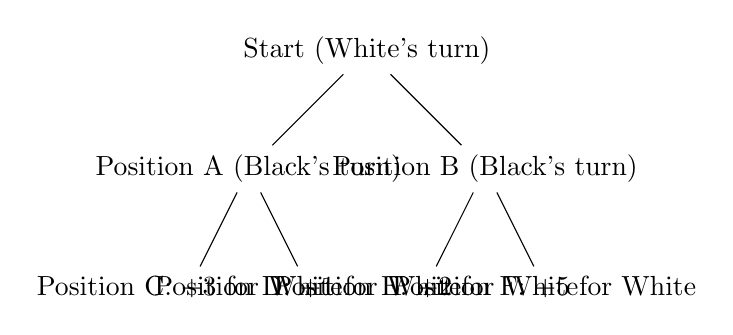
\begin{tikzpicture}[level distance=1.5cm,
  level 1/.style={sibling distance=3cm},
  level 2/.style={sibling distance=1.5cm}]
  \node {Start (White's turn)}
    child {node {Position A (Black's turn)}
      child {node {Position C: +3 for White}}
      child {node {Position D: +1 for White}}
    }
    child {node {Position B (Black's turn)}
      child {node {Position E: +2 for White}}
      child {node {Position F: +5 for White}}
    };
\end{tikzpicture}
\end{center}

In this example:
\begin{itemize}
    \item White has two possible moves from the start position, leading to positions A or B
    \item From position A, Black has two possible moves, leading to positions C or D
    \item From position B, Black has two possible moves, leading to positions E or F
    \item The numbers at the bottom are the evaluations (higher is better for White)
\end{itemize}

Using Minimax:
\begin{enumerate}
    \item If White chooses move A, Black will choose the move leading to position D (since +1 is worse for White than +3)
    \item If White chooses move B, Black will choose the move leading to position E (since +2 is worse for White than +5)
    \item So White's choices are effectively between positions D (+1) and E (+2)
    \item White will choose move B, leading to position E with a value of +2
\end{enumerate}

\subsubsection{Minimax with Depth}

The example above only looked one move ahead. In real chess, we want to look many moves ahead. We do this by applying Minimax recursively to a certain depth.

For example, if we set depth=4, the computer will look ahead 4 moves (2 moves by each player). The deeper we go, the better the computer will play, but the more calculations it needs to do.

\subsubsection{The Problem with Minimax}

The main problem with Minimax is that it grows exponentially with depth. In chess, each position has about 35 possible moves on average. So:
\begin{itemize}
    \item At depth 1: 35 positions to evaluate
    \item At depth 2: 35 × 35 = 1,225 positions
    \item At depth 3: 35 × 35 × 35 = 42,875 positions
    \item At depth 4: 35 × 35 × 35 × 35 = 1,500,625 positions
\end{itemize}

This quickly becomes too much for even the fastest computers. That's why we need more efficient algorithms, which we'll explore next.

\subsection{Alpha-Beta Pruning}

To make Minimax more efficient, we can use a technique called Alpha-Beta Pruning. This doesn't change the final decision, but it allows us to skip evaluating many positions that won't affect the outcome.

\subsubsection{How Alpha-Beta Pruning Works}

The key insight of Alpha-Beta Pruning is that once we find a good move, we can ignore moves that are clearly worse without fully evaluating them.

Let's go back to our example:

\begin{center}
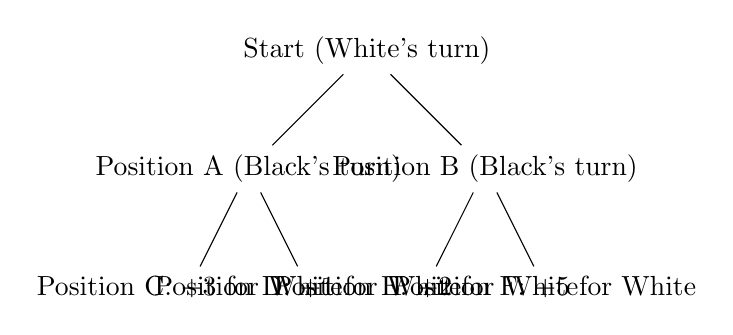
\begin{tikzpicture}[level distance=1.5cm,
  level 1/.style={sibling distance=3cm},
  level 2/.style={sibling distance=1.5cm}]
  \node {Start (White's turn)}
    child {node {Position A (Black's turn)}
      child {node {Position C: +3 for White}}
      child {node {Position D: +1 for White}}
    }
    child {node {Position B (Black's turn)}
      child {node {Position E: +2 for White}}
      child {node {Position F: +5 for White}}
    };
\end{tikzpicture}
\end{center}

With Alpha-Beta Pruning:
\begin{enumerate}
    \item White first explores move A
    \item Black's best response is move D, with value +1
    \item White then explores move B
    \item Black's first option is move E, with value +2
    \item Since +2 is already better than +1, White knows that move B is better than move A
    \item White doesn't need to explore Black's second option (move F) at all!
\end{enumerate}

In a real chess game with billions of possible positions, Alpha-Beta Pruning can eliminate huge portions of the search tree, allowing the computer to look much deeper in the same amount of time.

\subsubsection{Alpha-Beta Pruning in Code}

Here's a simplified version of how Alpha-Beta Pruning might be implemented in Python:

\begin{lstlisting}[style=Python]
def alpha_beta(position, depth, alpha, beta, maximizing_player):
    if depth == 0 or game_over(position):
        return evaluate(position)

    if maximizing_player:
        max_eval = float('-inf')
        for move in get_possible_moves(position):
            new_position = make_move(position, move)
            eval = alpha_beta(new_position, depth-1, alpha, beta, False)
            max_eval = max(max_eval, eval)
            alpha = max(alpha, eval)
            if beta <= alpha:
                break  # Beta cutoff
        return max_eval
    else:
        min_eval = float('inf')
        for move in get_possible_moves(position):
            new_position = make_move(position, move)
            eval = alpha_beta(new_position, depth-1, alpha, beta, True)
            min_eval = min(min_eval, eval)
            beta = min(beta, eval)
            if beta <= alpha:
                break  # Alpha cutoff
        return min_eval
\end{lstlisting}

The key part is the `if beta <= alpha: break` line, which is where we "prune" branches that won't affect the final decision.

\subsection{Monte Carlo Tree Search}

While Minimax with Alpha-Beta Pruning was the dominant approach in chess AI for decades, a newer algorithm called Monte Carlo Tree Search (MCTS) has become popular in recent years, especially for games like Go.

\subsubsection{How MCTS Works}

MCTS is based on random sampling. Instead of trying to evaluate every possible move, it plays many random games (simulations) from the current position and keeps track of which moves tend to lead to wins.

The algorithm has four main steps:
\begin{enumerate}
    \item \textbf{Selection}: Start from the root (current position) and select successive child nodes until reaching a leaf node. The selection is based on a formula that balances exploration (trying new moves) and exploitation (focusing on promising moves).

    \item \textbf{Expansion}: If the leaf node is not a terminal state (end of game), create one or more child nodes and select one.

    \item \textbf{Simulation}: Play a random game from the selected node until reaching a terminal state.

    \item \textbf{Backpropagation}: Update the statistics of all nodes in the path from the selected node to the root based on the result of the simulation.
\end{enumerate}

\subsubsection{MCTS Example}

Let's see a simple example of how MCTS might work in a chess-like game:

\begin{enumerate}
    \item We start at the current position and have three possible moves: A, B, and C.

    \item We haven't tried any of them yet, so we select move A (randomly).

    \item From position A, we play a random game until someone wins. Let's say White wins.

    \item We update the statistics for move A: 1 win out of 1 game.

    \item Next iteration, we select move B (to explore all options).

    \item From position B, we play a random game. Let's say Black wins.

    \item We update the statistics for move B: 0 wins out of 1 game.

    \item Next iteration, we select move C.

    \item From position C, we play a random game. Let's say White wins.

    \item We update the statistics for move C: 1 win out of 1 game.

    \item Now all moves have been tried once. In future iterations, we'll select based on which moves have the highest win rate, but also occasionally try moves with lower win rates (to make sure we don't miss anything).
\end{enumerate}

After many iterations (thousands or millions), we'll have a good estimate of which move is best.

\subsubsection{MCTS vs. Minimax}

MCTS has several advantages over Minimax:
\begin{itemize}
    \item It doesn't need an evaluation function (it just needs to know who won the game)
    \item It can be stopped at any time and will still give a reasonable move
    \item It naturally focuses on the most promising variations
    \item It handles uncertainty and randomness well
\end{itemize}

However, MCTS also has disadvantages:
\begin{itemize}
    \item It can miss tactical opportunities that Minimax would find
    \item It requires many simulations to be effective
    \item In games with a high branching factor (like chess), the random simulations might not be very informative
\end{itemize}

\subsubsection{MCTS in Code}

Here's a simplified version of how MCTS might be implemented in Python:

\begin{lstlisting}[style=Python]
import math
import random

class Node:
    def __init__(self, state, parent=None, move=None):
        self.state = state
        self.parent = parent
        self.move = move
        self.children = []
        self.wins = 0
        self.visits = 0
        self.untried_moves = get_possible_moves(state)

    def select_child(self):
        # UCB1 formula for selection
        s = sorted(self.children, key=lambda c: c.wins/c.visits +
                  math.sqrt(2*math.log(self.visits)/c.visits))
        return s[-1]  # Return the child with the highest UCB1 value

    def expand(self):
        move = self.untried_moves.pop()
        new_state = make_move(self.state, move)
        child = Node(new_state, self, move)
        self.children.append(child)
        return child

    def update(self, result):
        self.visits += 1
        self.wins += result

def monte_carlo_tree_search(root_state, iterations):
    root = Node(root_state)

    for _ in range(iterations):
        # Selection
        node = root
        while node.untried_moves == [] and node.children != []:
            node = node.select_child()

        # Expansion
        if node.untried_moves != []:
            node = node.expand()

        # Simulation
        state = node.state
        while not game_over(state):
            moves = get_possible_moves(state)
            move = random.choice(moves)
            state = make_move(state, move)

        # Backpropagation
        result = 1 if white_wins(state) else 0
        while node is not None:
            node.update(result)
            node = node.parent

    # Return the move with the highest number of visits
    return sorted(root.children, key=lambda c: c.visits)[-1].move
\end{lstlisting}

This is a basic implementation of MCTS. In practice, there are many optimizations and variations of this algorithm.

\section{Machine Learning for Chess}

So far, we've looked at traditional algorithms where humans explicitly program the rules for how the computer should play chess. Now, let's explore how computers can learn to play chess on their own through machine learning.

\subsection{From Handcrafted Rules to Learning}

Traditional chess engines like Stockfish use handcrafted evaluation functions created by chess experts. These functions consider factors like piece values, king safety, pawn structure, etc. While effective, creating and tuning these functions requires a lot of human expertise.

Machine learning takes a different approach: instead of telling the computer exactly how to evaluate positions, we let it learn from data. This has several advantages:
\begin{itemize}
    \item The computer might discover patterns that humans haven't noticed
    \item The evaluation can be more nuanced and adapt to different styles of play
    \item We don't need chess experts to create the evaluation function
\end{itemize}

\subsection{Neural Networks}

The most common type of machine learning model used in modern chess AI is the neural network. Neural networks are loosely inspired by how the human brain works, with interconnected "neurons" that process information.

\subsubsection{How Neural Networks Work}

A neural network consists of layers of neurons:
\begin{itemize}
    \item \textbf{Input Layer}: Receives the initial data (in chess, this would be the board position)
    \item \textbf{Hidden Layers}: Process the information through a series of mathematical operations
    \item \textbf{Output Layer}: Produces the final result (in chess, this might be an evaluation of the position or a probability distribution over possible moves)
\end{itemize}

Each neuron takes inputs from the previous layer, applies weights to them, sums them up, and then applies an "activation function" to produce its output. The weights are what the network learns during training.

\subsubsection{Neural Network Example}

Here's a simple example of how a neural network might evaluate a chess position:

\begin{enumerate}
    \item \textbf{Input}: The board position, represented as a 64-element array (one for each square), where each element indicates what piece (if any) is on that square.

    \item \textbf{Hidden Layer 1}: Might learn to recognize patterns like "knight fork" or "queen in danger."

    \item \textbf{Hidden Layer 2}: Might combine these patterns to understand concepts like "attacking position" or "defensive structure."

    \item \textbf{Output}: A single number representing the evaluation of the position (positive for White advantage, negative for Black advantage).
\end{enumerate}

\subsubsection{Training Neural Networks}

Neural networks learn by adjusting their weights based on examples. For chess, we might train a network by:
\begin{itemize}
    \item Showing it millions of positions from real games
    \item For each position, telling it who eventually won the game
    \item Adjusting the weights so that the network's evaluation better predicts the winner
\end{itemize}

This process is called "supervised learning" because we're supervising the network by providing the correct answers.

\subsection{Reinforcement Learning}

While supervised learning is powerful, it requires a large dataset of labeled examples. Reinforcement learning (RL) is another approach where the computer learns by playing against itself and receiving rewards for good moves.

\subsubsection{How Reinforcement Learning Works}

In reinforcement learning:
\begin{enumerate}
    \item The agent (our chess AI) observes the current state (the board position)
    \item It takes an action (makes a move)
    \item It receives a reward (e.g., +1 for winning, -1 for losing, 0 for drawing)
    \item It updates its policy (strategy for choosing moves) to maximize future rewards
\end{enumerate}

The key insight is that the agent doesn't need to be told exactly what to do in each situation. It learns through trial and error, gradually improving its policy.

\subsubsection{Policy and Value Functions}

In reinforcement learning for chess, we typically have two main components:
\begin{itemize}
    \item \textbf{Policy Function}: Decides which move to make in a given position
    \item \textbf{Value Function}: Estimates how good a position is
\end{itemize}

Both of these can be represented by neural networks:
\begin{itemize}
    \item The policy network takes a board position as input and outputs a probability distribution over possible moves
    \item The value network takes a board position as input and outputs an estimate of who will win from that position
\end{itemize}

\subsubsection{Self-Play}

One of the most effective ways to train a reinforcement learning agent for chess is through self-play:
\begin{enumerate}
    \item Start with a randomly initialized policy
    \item Have the agent play games against itself
    \item Use the outcomes of these games to improve the policy
    \item Repeat with the improved policy
\end{enumerate}

This approach was used by AlphaZero, a chess AI developed by DeepMind that famously defeated Stockfish (one of the strongest traditional chess engines) after learning to play chess in just 24 hours of self-play.

\section{Deep Reinforcement Learning}
\subsection{PPO Algorithm: From Basics to Advanced}

\subsubsection{Understanding Reinforcement Learning Basics}

Before diving into PPO, let's understand the basic reinforcement learning concepts. Imagine you're teaching a child to play chess:

\begin{enumerate}
    \item The child looks at the chess board (this is the \textbf{state} $s$)
    \item The child makes a move (this is the \textbf{action} $a$)
    \item You tell them if the move was good or bad (this is the \textbf{reward} $r$)
    \item The board changes to a new position (this is the \textbf{next state} $s'$)
    \item This process repeats until the game ends
\end{enumerate}

In mathematical terms, at each timestep $t$, the agent:
\begin{itemize}
    \item Observes state $s_t$
    \item Takes action $a_t$
    \item Receives reward $r_t$
    \item Transitions to state $s_{t+1}$
\end{itemize}

The goal is to find a policy $\pi(a|s)$ that maximizes the expected cumulative reward:

\begin{equation}
    J(\pi) = \mathbb{E}_{\tau \sim \pi} \left[ \sum_{t=0}^{T} \gamma^t r_t \right]
\end{equation}

Where:
\begin{itemize}
    \item $\pi(a|s)$ is our policy - it tells us the probability of taking action $a$ in state $s$
    \item $\tau$ is a trajectory (a complete sequence of states, actions, and rewards)
    \item $\gamma$ is a discount factor (value between 0 and 1) that makes future rewards worth less than immediate rewards
    \item $r_t$ is the reward at time step $t$
    \item $T$ is the time horizon (length of the game)
    \item $\mathbb{E}_{\tau \sim \pi}$ means the expected value over all possible trajectories when following policy $\pi$
\end{itemize}

\subsubsection*{Example with Chess}
Imagine a simple chess scenario:
\begin{itemize}
    \item You capture an opponent's pawn (+1 reward)
    \item Two moves later, you capture a knight (+3 reward)
    \item Three moves after that, you capture the queen (+9 reward)
    \item Finally, after two more moves, you checkmate (+50 reward)
\end{itemize}

With a discount factor $\gamma = 0.9$, your cumulative discounted reward would be:
\begin{align*}
    J &= 1 + 0.9^2 \times 3 + 0.9^5 \times 9 + 0.9^7 \times 50 \\
    &= 1 + 0.81 \times 3 + 0.59049 \times 9 + 0.47829 \times 50 \\
    &= 1 + 2.43 + 5.31 + 23.91 \\
    &= 32.65
\end{align*}

If we didn't use discounting ($\gamma = 1$), the sum would simply be $1 + 3 + 9 + 50 = 63$. The discounting makes immediate rewards more valuable than delayed rewards, encouraging the agent to achieve goals sooner rather than later.

\subsubsection{Value Functions and Advantages}

We use two important functions in reinforcement learning:
\begin{itemize}
    \item \textbf{Value function} $V^\pi(s)$: How good is it to be in state $s$? This estimates the total expected future reward from being in state $s$ and following policy $\pi$ afterward.
    \item \textbf{Q-function} $Q^\pi(s,a)$: How good is it to take action $a$ in state $s$? This estimates the total expected future reward from taking action $a$ in state $s$ and then following policy $\pi$ afterward.
\end{itemize}

Mathematically:
\begin{equation}
    V^\pi(s) = \mathbb{E}_{\tau \sim \pi} \left[ \sum_{t=0}^{T} \gamma^t r_t | s_0 = s \right]
\end{equation}

This equation means: "What's the expected total reward if I start in state $s$ and follow policy $\pi$ all the way to the end of the game?"

\begin{equation}
    Q^\pi(s,a) = \mathbb{E}_{\tau \sim \pi} \left[ \sum_{t=0}^{T} \gamma^t r_t | s_0 = s, a_0 = a \right]
\end{equation}

This equation means: "What's the expected total reward if I take action $a$ in state $s$ right now, and then follow policy $\pi$ all the way to the end of the game?"

\subsubsection*{Chess Example for Value Function}
Imagine you're evaluating a chess position:
\begin{itemize}
    \item Position A: You have a queen advantage, and your opponent's king is exposed. Value function might estimate: $V(\text{Position A}) = +8$ (very good for you)
    \item Position B: Equal material, but your pieces are poorly positioned. Value function might estimate: $V(\text{Position B}) = -1$ (slightly bad for you)
\end{itemize}

\subsubsection*{Chess Example for Q-Function}
For a given position, different moves have different Q-values:
\begin{itemize}
    \item Move 1: Capture opponent's queen with your knight. $Q(\text{Position}, \text{Capture Queen}) = +7$ (excellent move)
    \item Move 2: Move your pawn forward one square. $Q(\text{Position}, \text{Advance Pawn}) = +0.5$ (slightly good move)
    \item Move 3: Move your king into check. $Q(\text{Position}, \text{King into Check}) = -10$ (terrible move)
\end{itemize}

The \textbf{advantage function} tells us how much better an action is compared to the average action:
\begin{equation}
    A^\pi(s,a) = Q^\pi(s,a) - V^\pi(s)
\end{equation}

This is extremely important because it tells us which actions are better than the average action in a given state. It's the key to learning which actions to prefer.

\subsubsection*{Chess Example for Advantage Function}
Imagine a position where the overall value is $V(\text{Position}) = +2$ (slightly good for you). For different moves:
\begin{itemize}
    \item Move 1: Capture opponent's queen. $Q(\text{Position}, \text{Capture Queen}) = +9$
    $\Rightarrow$ Advantage = $Q(\text{Position}, \text{Capture Queen}) - V(\text{Position}) = +9 - (+2) = +7$ (much better than average)
    
    \item Move 2: Move pawn forward. $Q(\text{Position}, \text{Advance Pawn}) = +2$
    $\Rightarrow$ Advantage = $Q(\text{Position}, \text{Advance Pawn}) - V(\text{Position}) = +2 - (+2) = 0$ (exactly average)
    
    \item Move 3: Blunder your bishop. $Q(\text{Position}, \text{Blunder Bishop}) = -3$
    $\Rightarrow$ Advantage = $Q(\text{Position}, \text{Blunder Bishop}) - V(\text{Position}) = -3 - (+2) = -5$ (much worse than average)
\end{itemize}

The agent will learn to prefer actions with positive advantage and avoid actions with negative advantage.

\subsubsection{From Basic RL to PPO}

Proximal Policy Optimization (PPO) is an advanced reinforcement learning algorithm that makes learning more stable and efficient. Imagine PPO as a smart robot learning to play chess. Let's break it down into simple parts:

\begin{figure}[h]
    \centering
    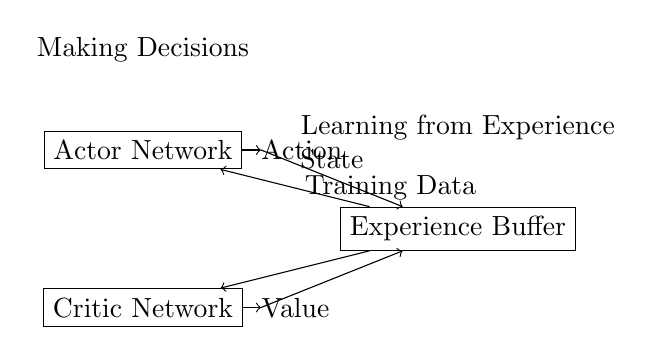
\begin{tikzpicture}
        \node[draw, rectangle] (actor) at (0,2) {Actor Network};
        \node[draw, rectangle] (critic) at (0,0) {Critic Network};
        \node[draw, rectangle] (buffer) at (4,1) {Experience Buffer};
        
        \draw[->] (actor) -- node[right] {Action} (1.5,2);
        \draw[->] (critic) -- node[right] {Value} (1.5,0);
        \draw[->] (1.5,2) -- node[above] {State} (buffer);
        \draw[->] (1.5,0) -- (buffer);
        \draw[->] (buffer) -- node[right] {Training Data} (actor);
        \draw[->] (buffer) -- (critic);
        
        \node[above] at (0,3) {Making Decisions};
        \node[above] at (4,2) {Learning from Experience};
    \end{tikzpicture}
    \caption{PPO Architecture}
    \label{fig:ppo_architecture}
\end{figure}

\subsubsection{The Actor Network}
Think of the Actor as a smart chess player who decides which moves to make. It looks at the chess board (state) and chooses the best move based on what it has learned.

\subsubsection{The Critic Network}
The Critic is like a coach who tells the Actor if its moves were good or bad. It gives feedback about how well the move might work.

\subsubsection{Experience Buffer}
The Buffer is like a notebook where the robot writes down all its experiences. It remembers:
\begin{itemize}
    \item What moves it made (actions)
    \item How good those moves were (values)
    \item What happened after each move (rewards)
\end{itemize}

\subsection{How PPO Learns}

PPO learns through a process called "self-play." Here's how it works:

\begin{enumerate}
    \item The robot plays many games against itself
    \item It records every move and what happened
    \item The Critic evaluates how good each move was
    \item The Actor learns from this feedback
    \item The process repeats, getting better each time
\end{enumerate}

\begin{figure}[h]
    \centering
    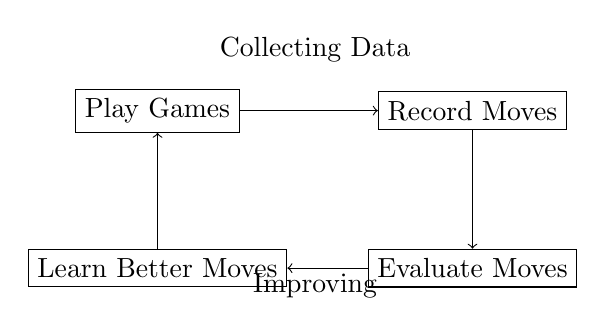
\begin{tikzpicture}
        \node[draw, rectangle] (play) at (0,2) {Play Games};
        \node[draw, rectangle] (record) at (4,2) {Record Moves};
        \node[draw, rectangle] (evaluate) at (4,0) {Evaluate Moves};
        \node[draw, rectangle] (learn) at (0,0) {Learn Better Moves};
        
        \draw[->] (play) -- (record);
        \draw[->] (record) -- (evaluate);
        \draw[->] (evaluate) -- (learn);
        \draw[->] (learn) -- (play);
        
        \node[above] at (2,2.5) {Collecting Data};
        \node[above] at (2,-0.5) {Improving};
    \end{tikzpicture}
    \caption{PPO Learning Process}
    \label{fig:ppo_learning}
\end{figure}

\subsection{Key Components}

\subsubsection{Buffer}
The Buffer stores all the robot's experiences. It's like a big memory box that helps the robot remember:
\begin{itemize}
    \item States: Different chess board positions
    \item Actions: Moves that were made
    \item Rewards: How good the moves were
    \item Advantages: How much better a move was than average
\end{itemize}

\subsubsection{Learning Process}

The learning process has several important steps:
\begin{enumerate}
    \item \textbf{Action Selection}: The robot decides what move to make
    \item \textbf{Value Estimation}: It guesses how good the move might be
    \item \textbf{Experience Collection}: It records what happens
    \item \textbf{Training}: It learns from its experiences
\end{enumerate}

\subsection{The PPO Algorithm in Detail}

\subsubsection{The PPO Objective Function}

PPO introduces a clever way to update the policy without making too large changes. The key innovation is the PPO objective function:

\begin{equation}
    L^{CLIP}(\theta) = \mathbb{E}_t \left[ \min(r_t(\theta) A_t, \text{clip}(r_t(\theta), 1-\epsilon, 1+\epsilon) A_t) \right]
\end{equation}

Where:
\begin{itemize}
    \item $r_t(\theta) = \frac{\pi_\theta(a_t|s_t)}{\pi_{\theta_{old}}(a_t|s_t)}$ is the probability ratio between the new and old policies
    \item $A_t$ is the advantage estimate for action $a_t$ in state $s_t$
    \item $\epsilon$ is a hyperparameter (typically 0.1 or 0.2) that limits how much the policy can change in a single update
    \item $\text{clip}(r_t(\theta), 1-\epsilon, 1+\epsilon)$ clips the ratio to be between $[1-\epsilon, 1+\epsilon]$
\end{itemize}

\subsubsection*{Breaking Down the PPO Formula}

To really understand PPO, let's break it down step-by-step:

1. \textbf{Probability Ratio}: $r_t(\theta) = \frac{\pi_\theta(a_t|s_t)}{\pi_{\theta_{old}}(a_t|s_t)}$ compares how likely an action is under the new policy versus the old policy.
   - If $r_t = 1$: The new policy thinks this action is just as good as the old policy did
   - If $r_t = 1.5$: The new policy thinks this action is 50\% better than the old policy did
   - If $r_t = 0.7$: The new policy thinks this action is 30\% worse than the old policy did

2. \textbf{The Clipping Mechanism}: $\text{clip}(r_t(\theta), 1-\epsilon, 1+\epsilon)$ prevents the ratio from being too far from 1.
   - If $\epsilon = 0.2$ and $r_t = 1.3$, the clipped value is still 1.2 (within bounds)
   - If $\epsilon = 0.2$ and $r_t = 1.5$, the clipped value becomes 1.2 (clipped down)
   - If $\epsilon = 0.2$ and $r_t = 0.7$, the clipped value is still 0.7 (within bounds)
   - If $\epsilon = 0.2$ and $r_t = 0.6$, the clipped value becomes 0.8 (clipped up)

3. \textbf{The Min Operation}: $\min(r_t(\theta) A_t, \text{clip}(r_t(\theta), 1-\epsilon, 1+\epsilon) A_t)$ makes training even more conservative.

\subsubsection*{Chess Example of PPO in Action}

Let's see how PPO works with a chess example:

Suppose our chess agent considers a move "Capture opponent's knight with bishop":

\begin{itemize}
    \item The old policy: $\pi_{\theta_{old}}(\text{capture knight}|\text{current board}) = 0.2$ (20\% probability)
    \item The new policy: $\pi_{\theta}(\text{capture knight}|\text{current board}) = 0.4$ (40\% probability)
    \item The ratio: $r_t = \frac{0.4}{0.2} = 2.0$ (the new policy thinks this move is twice as good)
    \item The advantage: $A_t = +3$ (this is actually a good move)
    \item With $\epsilon = 0.2$, the clipped ratio is $\min(2.0, 1.2) = 1.2$
\end{itemize}

So our PPO update will be:
\begin{align*}
    \min(r_t A_t, \text{clip}(r_t) A_t) &= \min(2.0 \times 3, 1.2 \times 3) \\
    &= \min(6.0, 3.6) \\
    &= 3.6
\end{align*}

Instead of updating with a factor of $6.0$ (which could be unstable), we update with $3.6$, making the learning more stable.

Now consider a different move "Move pawn forward unnecessarily":

\begin{itemize}
    \item Advantage: $A_t = -2$ (this is a bad move)
    \item Old policy probability: $\pi_{\theta_{old}}(\text{move pawn}|\text{board}) = 0.1$
    \item New policy probability: $\pi_{\theta}(\text{move pawn}|\text{board}) = 0.05$
    \item Ratio: $r_t = \frac{0.05}{0.1} = 0.5$
    \item With $\epsilon = 0.2$, the clipped ratio is $\max(0.5, 0.8) = 0.8$
\end{itemize}

Our PPO update would be:
\begin{align*}
    \min(r_t A_t, \text{clip}(r_t) A_t) &= \min(0.5 \times (-2), 0.8 \times (-2)) \\
    &= \min(-1.0, -1.6) \\
    &= -1.0
\end{align*}

Here, we use the unclipped value because it gives a less negative result (remember we're trying to maximize our objective).

This clipping mechanism is why PPO is so effective - it prevents wild swings in the policy during training, leading to more stable and reliable learning.

\subsubsection{Generalized Advantage Estimation (GAE)}

Calculating advantages accurately is crucial for PPO to work well. PPO uses a technique called Generalized Advantage Estimation (GAE) to calculate better advantage estimates:

\begin{equation}
    A^{GAE(\gamma, \lambda)}_t = \sum_{l=0}^{\infty} (\gamma \lambda)^l \delta_{t+l}
\end{equation}

Where $\delta_t = r_t + \gamma V(s_{t+1}) - V(s_t)$ is the temporal difference (TD) error.

\subsubsection*{Understanding TD Error}

The temporal difference error $\delta_t$ can be understood as "how surprised we were by the reward". It compares:
\begin{itemize}
    \item What we actually got: $r_t + \gamma V(s_{t+1})$ (immediate reward plus discounted value of next state)
    \item What we expected: $V(s_t)$ (our estimate of the current state's value)
\end{itemize}

If $\delta_t > 0$, the action was better than expected. If $\delta_t < 0$, the action was worse than expected.

\subsubsection*{The GAE Formula Explained}

GAE computes advantage by looking at a weighted sum of all future TD errors:
\begin{itemize}
    \item $\delta_t$ gets full weight
    \item $\delta_{t+1}$ gets weight $(\gamma \lambda)$
    \item $\delta_{t+2}$ gets weight $(\gamma \lambda)^2$
    \item And so on...
\end{itemize}

In practice, we compute this recursively, starting from the end of an episode and working backward:
\begin{equation}
    A_t = \delta_t + \gamma \lambda A_{t+1}
\end{equation}

\subsubsection*{Chess Example of GAE}

Let's see how GAE works with a chess example. Imagine we're tracking a 3-move sequence with $\gamma = 0.9$ and $\lambda = 0.95$:

\begin{itemize}
    \item Move 1: Advance pawn
        \begin{itemize}
            \item Reward $r_1 = 0$ (no immediate benefit)
            \item Current state value $V(s_1) = 2$ (slightly good position)
            \item Next state value $V(s_2) = 3$ (better position after pawn move)
            \item TD error: $\delta_1 = 0 + 0.9 \times 3 - 2 = 0.7$ (slightly better than expected)
        \end{itemize}
    
    \item Move 2: Capture opponent's knight
        \begin{itemize}
            \item Reward $r_2 = 3$ (captured a knight worth 3 points)
            \item Current state value $V(s_2) = 3$
            \item Next state value $V(s_3) = 5$ (even better position)
            \item TD error: $\delta_2 = 3 + 0.9 \times 5 - 3 = 4.5$ (much better than expected)
        \end{itemize}
    
    \item Move 3: Set up checkmate
        \begin{itemize}
            \item Reward $r_3 = 0$ (no immediate capture)
            \item Current state value $V(s_3) = 5$
            \item Next state value $V(s_4) = 9$ (winning position)
            \item TD error: $\delta_3 = 0 + 0.9 \times 9 - 5 = 3.1$ (better than expected)
        \end{itemize}
\end{itemize}

Now we calculate the advantages backwards:
\begin{align*}
    A_3 &= \delta_3 = 3.1 \\
    A_2 &= \delta_2 + \gamma \lambda A_3 = 4.5 + 0.9 \times 0.95 \times 3.1 \approx 7.14 \\
    A_1 &= \delta_1 + \gamma \lambda A_2 = 0.7 + 0.9 \times 0.95 \times 7.14 \approx 6.84
\end{align*}

Notice how the advantage of the first move ($A_1 = 6.84$) is very high, even though its immediate TD error was small ($\delta_1 = 0.7$). This is because GAE correctly assigns credit to the first move for setting up the subsequent good moves.

\section{Chess Environment Representation}

\subsection{How Chess is Represented for the AI}

Before we can teach an AI to play chess, we need to represent the chess board in a way the computer can understand. Let's explore how the chess environment is implemented.

\subsubsection{Board Representation}

The chess board is represented as a multi-dimensional array. Each position on the board contains information about:

\begin{itemize}
    \item What piece is on that square (pawn, knight, bishop, rook, queen, king, or empty)
    \item Which player owns that piece (white or black)
    \item Special states like whether a king has castling rights or if a pawn can be captured en passant
\end{itemize}

\begin{figure}[h]
    \centering
    \begin{tikzpicture}[scale=1.2]
        % Define colors
        \colorlet{light}{white}
        \colorlet{dark}{black!60}
        
        % Draw the checkered board
        \foreach \i in {0,...,7} {
            \foreach \j in {0,...,7} {
                \pgfmathsetmacro{\colorfill}{mod(\i+\j,2) ? "light" : "dark"}
                \fill[\colorfill] (\i*0.6,\j*0.6) rectangle +(0.6,0.6);
                \node[font=\tiny] at (\i*0.6+0.1, \j*0.6+0.1) {$c_{\i,\j}$};
            }
        }
        
        % Add file labels (a-h) at the bottom
        \foreach \i [count=\xi from 0] in {a,...,h}
            \node at (\xi*0.6+0.3, -0.2) {\i};
            
        % Add rank labels (1-8) on the left
        \foreach \i [count=\xi from 0] in {1,...,8}
            \node at (-0.2, \xi*0.6-0.3) {\i};
        
        % Add some sample pieces
        \node at (0*0.6+0.3, 0*0.6+0.3) {\LARGE ♜}; % Black rook
        \node at (1*0.6+0.3, 0*0.6+0.3) {\LARGE ♞}; % Black knight
        \node at (0*0.6+0.3, 1*0.6+0.3) {\LARGE ♟}; % Black pawn
        
        \node at (6*0.6+0.3, 6*0.6+0.3) {\LARGE ♙}; % White pawn
        \node at (7*0.6+0.3, 7*0.6+0.3) {\LARGE ♖}; % White rook
        \node at (6*0.6+0.3, 7*0.6+0.3) {\LARGE ♘}; % White knight
        \node at (4*0.6+0.3, 7*0.6+0.3) {\LARGE ♔}; % White king
        \node at (3*0.6+0.3, 7*0.6+0.3) {\LARGE ♕}; % White queen
    \end{tikzpicture}
    \caption{A chess board with pieces and coordinates $c_{x,y}$}
    \label{fig:chess_array}
\end{figure}

\subsubsection{State Encoding}

To feed the board state into our neural networks, we encode it as a multi-channel 2D array. Each channel represents different information:

\begin{itemize}
    \item Channel 1-6: White pieces (pawn, knight, bishop, rook, queen, king)
    \item Channel 7-12: Black pieces (pawn, knight, bishop, rook, queen, king)
    \item Additional channels for special information (whose turn it is, castling rights, etc.)
\end{itemize}

Here's a simplified example of how we represent a white pawn at position (2,1):

\begin{lstlisting}[style=Python]
# Channel 1 (White Pawns)
board[0, 2, 1] = 1  # Set to 1 for white pawn at position (2,1)
\end{lstlisting}

\subsubsection{Move Encoding}

Chess moves are encoded as integers from 0 to 4095, representing all possible combinations of:
\begin{itemize}
    \item Starting square (64 possibilities)
    \item Ending square (64 possibilities)
    \item Special move types (promotion to knight, bishop, rook, or queen)
\end{itemize}

In our implementation, we map this to an action space of 0-4095, but we also use a move mask to ensure only legal moves are selected.

\begin{lstlisting}[style=Python]
def encode_move(from_square, to_square, promotion=None):
    # Convert chess squares to 0-63 indices
    from_idx = from_square.index
    to_idx = to_square.index
    
    # Base move encoding
    move_code = from_idx * 64 + to_idx
    
    # Add promotion information if applicable
    if promotion:
        if promotion == chess.QUEEN:
            move_code += 1 * 4096
        elif promotion == chess.ROOK:
            move_code += 2 * 4096
        elif promotion == chess.BISHOP:
            move_code += 3 * 4096
        elif promotion == chess.KNIGHT:
            move_code += 4 * 4096
    
    return move_code
\end{lstlisting}

\subsection{Action Masking}

A critical aspect of the chess environment is action masking. Since chess has very specific rules about which moves are legal, we use an action mask to ensure the AI only selects legal moves:

\begin{lstlisting}[style=Python]
def get_action_mask(board):
    # Initialize mask with zeros (all moves illegal by default)
    mask = np.zeros(4096, dtype=np.float32)
    
    # For each legal move, set the corresponding mask value to 1
    for move in board.legal_moves:
        move_idx = encode_move(move.from_square, move.to_square, move.promotion)
        mask[move_idx] = 1.0
    
    return mask
\end{lstlisting}

This mask is fed into the neural network along with the board state. The network then outputs probabilities only for legal moves by multiplying its raw output with this mask.

\section{Neural Network Architecture in Detail}

\subsection{Detailed Implementation}

Let's see how PPO is implemented in our chess project. Here's how the core components work together:

\subsection{The Actor Network: How the AI Decides Where to Move}

The Actor Network is like the AI's "chess intuition" - it looks at the board and decides which move to make. Let's break down how it works in detail:

\begin{lstlisting}[style=Python]
class Actor(nn.Module):
    def __init__(self, state_dim, action_dim, hidden_layers):
        super().__init__()
        
        # Create network layers
        layers = []
        prev_dim = state_dim
        
        # Add hidden layers with ReLU activation
        for dim in hidden_layers:
            layers.append(nn.Linear(prev_dim, dim))
            layers.append(nn.ReLU())
            prev_dim = dim
        
        # Output layer with softmax for action probabilities
        layers.append(nn.Linear(prev_dim, action_dim))
        layers.append(nn.Softmax(dim=-1))
        
        self.model = nn.Sequential(*layers)
        
    def forward(self, state, action_mask):
        # Get probabilities for all actions
        probs = self.model(state)
        
        # Apply mask to only allow valid moves
        probs = probs * action_mask
        
        # Normalize probabilities
        probs = probs / (probs.sum(dim=1, keepdim=True) + 1e-10)
        
        # Create a categorical distribution
        dist = Categorical(probs)
        return dist
\end{lstlisting}

\subsubsection*{Understanding the Actor Network Step by Step}

% --- Figure 6: Make it full-width and improve TikZ layout ---
\onecolumn

\begin{figure}[!htbp]
    \centering
    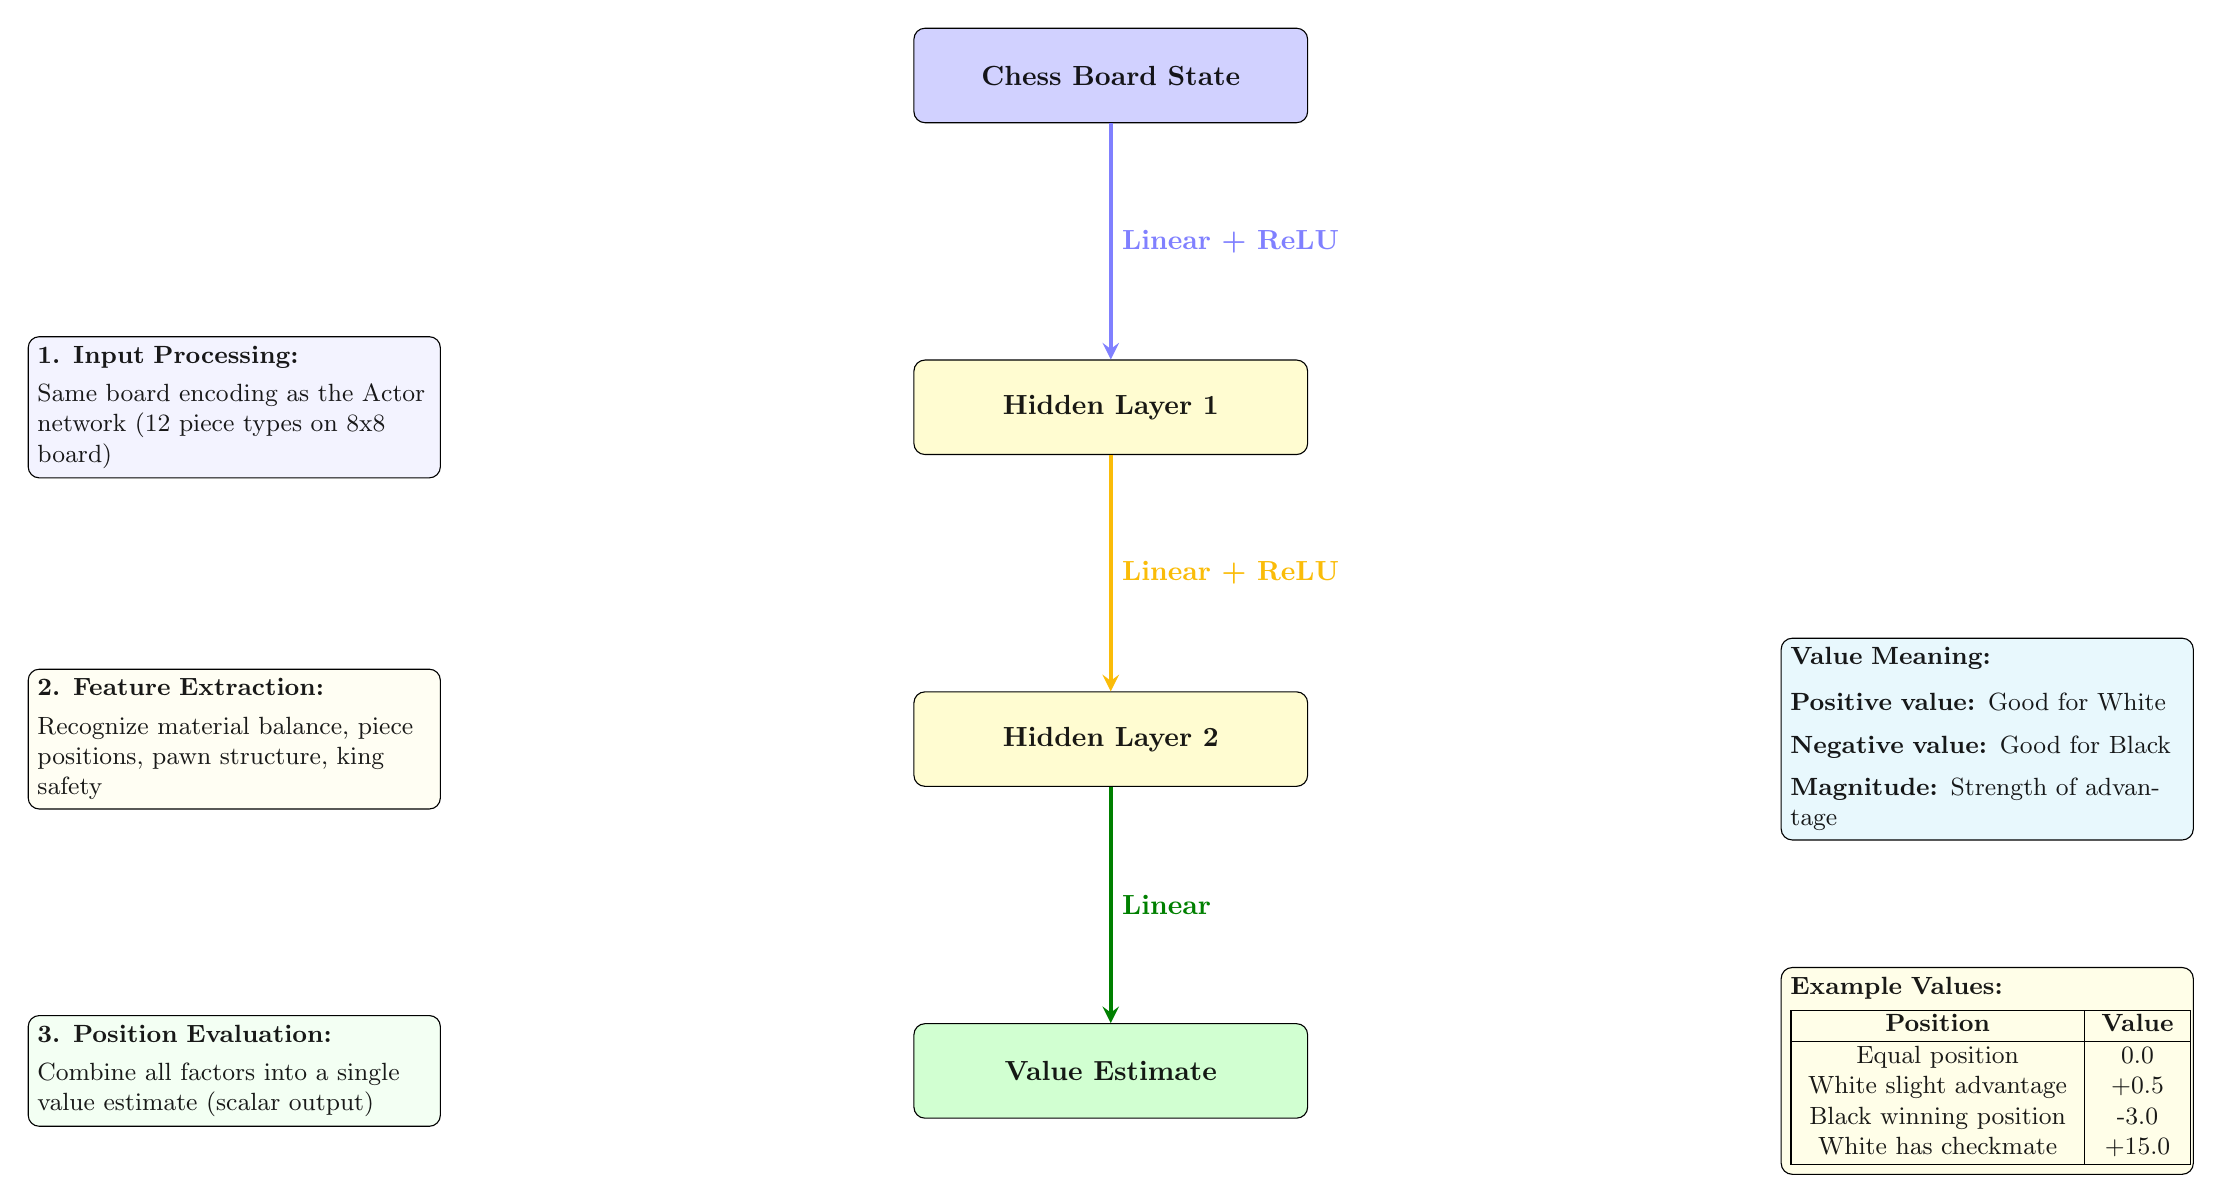
\begin{tikzpicture}[
        scale=1.0,
        transform shape,
        node distance=3cm,
        every node/.style={transform shape},
        block/.style={draw, rectangle, rounded corners, minimum width=5cm, minimum height=1.2cm, align=center, fill opacity=0.9},
        note/.style={draw, rounded corners, fill opacity=0.9, text width=5cm, align=left, font=\small}
    ]
        % Main network components
        \node[block, fill=blue!20] (input) at (0,0) {\textbf{Chess Board State}};
        \node[block, fill=yellow!20] (hidden1) [below=of input] {\textbf{Hidden Layer 1}};
        \node[block, fill=yellow!20] (hidden2) [below=of hidden1] {\textbf{Hidden Layer 2}};
        \node[block, fill=green!20] (output) [below=of hidden2] {\textbf{Value Estimate}};

        % Processing steps on the left
        \node[note, fill=blue!5] (step1) [left=6cm of hidden1] {\textbf{1. Input Processing:}\\[0.1cm]Same board encoding as the Actor\\network (12 piece types on 8x8 board)};
        \node[note, fill=yellow!5] (step2) [left=6cm of hidden2] {\textbf{2. Feature Extraction:}\\[0.1cm]Recognize material balance, piece\\positions, pawn structure, king safety};
        \node[note, fill=green!5] (step3) [left=6cm of output] {\textbf{3. Position Evaluation:}\\[0.1cm]Combine all factors into a single\\value estimate (scalar output)};

        % Value explanation on the right
        \node[note, fill=cyan!10] (value) [right=6cm of hidden2] {\textbf{Value Meaning:}\\[0.2cm]\textbf{Positive value:} Good for White\\[0.15cm]\textbf{Negative value:} Good for Black\\[0.15cm]\textbf{Magnitude:} Strength of advantage};

        % Example values table
        \node[note, fill=yellow!10] (example) [right=6cm of output] {
            \textbf{Example Values:}\\[0.1cm]
            \begin{tabular}{|c|c|}
                \hline
                \textbf{Position} & \textbf{Value} \\
                \hline
                Equal position & 0.0 \\
                White slight advantage & +0.5 \\
                Black winning position & -3.0 \\
                White has checkmate & +15.0 \\
                \hline
            \end{tabular}
        };

        % Connect nodes with descriptive labels
        \draw[->, ultra thick, >=stealth, blue!50] (input) -- node[right, align=left, font=\normalsize] {\textbf{Linear + ReLU}} (hidden1);
        \draw[->, ultra thick, >=stealth, yellow!50!orange] (hidden1) -- node[right, align=left, font=\normalsize] {\textbf{Linear + ReLU}} (hidden2);
        \draw[->, ultra thick, >=stealth, green!50!black] (hidden2) -- node[right, align=left, font=\normalsize] {\textbf{Linear}} (output);
    \end{tikzpicture}
    \caption{Actor Network data flow (vertical layout)}
    \label{fig:actor_flow}
\end{figure}

\twocolumn

1. \textbf{Input Processing}: The network takes the chess board state as input (encoded as described earlier).

2. \textbf{Hidden Layers}: The state passes through multiple hidden layers with ReLU activation functions. Each layer helps the network recognize different patterns:
   - \textbf{First layer}: Recognizes basic patterns like piece positions
   - \textbf{Deeper layers}: Recognize more complex patterns like pawn structures, attacking threats, or defensive formations

3. \textbf{Output Layer}: Produces a probability for each possible move (all 4096 possible moves).

4. \textbf{Action Masking}: The network multiplies its output by the action mask, which has 1s for legal moves and 0s for illegal moves. This ensures only legal moves get non-zero probabilities.

5. \textbf{Normalization}: The probabilities are normalized to sum to 1.

6. \textbf{Distribution Creation}: The final normalized probabilities are used to create a categorical distribution, which allows the agent to sample actions based on their probabilities.

\subsubsection*{Concrete Example of Actor Network Processing}

Imagine the current chess position has these legal moves with the following raw probabilities from the network:

\begin{center}
\begin{tabular}{|c|c|c|}
\hline
\textbf{Move} & \textbf{Raw Probability} & \textbf{After Masking} \\
\hline
e2e4 (Pawn to e4) & 0.15 & 0.15 \\
\hline
d2d4 (Pawn to d4) & 0.12 & 0.12 \\
\hline
g1f3 (Knight to f3) & 0.08 & 0.08 \\
\hline
e1g1 (Castle kingside) & 0.05 & 0.05 \\
\hline
All other legal moves & 0.20 total & 0.20 total \\
\hline
All illegal moves & 0.40 total & 0.00 (masked out) \\
\hline
\end{tabular}
\end{center}

After normalization, the probabilities become:
\begin{center}
\begin{tabular}{|c|c|}
\hline
\textbf{Move} & \textbf{Normalized Probability} \\
\hline
e2e4 (Pawn to e4) & $0.15 / 0.60 = 0.25$ (25\%) \\
\hline
d2d4 (Pawn to d4) & $0.12 / 0.60 = 0.20$ (20\%) \\
\hline
g1f3 (Knight to f3) & $0.08 / 0.60 = 0.13$ (13\%) \\
\hline
e1g1 (Castle kingside) & $0.05 / 0.60 = 0.08$ (8\%) \\
\hline
All other legal moves & $0.20 / 0.60 = 0.33$ (33\%) \\
\hline
\end{tabular}
\end{center}

The agent would then sample from this distribution, with e2e4 having the highest chance (25\%) of being selected.

\subsection{The Critic Network: How the AI Evaluates Positions}

While the Actor decides what moves to make, the Critic evaluates how good the current chess position is. It's like having a chess expert who can look at a board and tell you "This position is good for white" or "Black has an advantage here."

\begin{lstlisting}[style=Python]
class Critic(nn.Module):
    def __init__(self, state_dim, hidden_layers):
        super().__init__()
        
        # Create network layers
        layers = []
        prev_dim = state_dim
        
        # Add hidden layers with ReLU activation
        for dim in hidden_layers:
            layers.append(nn.Linear(prev_dim, dim))
            layers.append(nn.ReLU())
            prev_dim = dim
        
        # Output a single value estimate
        layers.append(nn.Linear(prev_dim, 1))
        
        self.model = nn.Sequential(*layers)
        
    def forward(self, state):
        # Return the estimated value of this state
        return self.model(state)
\end{lstlisting}

\subsubsection*{Understanding the Critic Network Step by Step}

\begin{figure}[p]
    \centering
    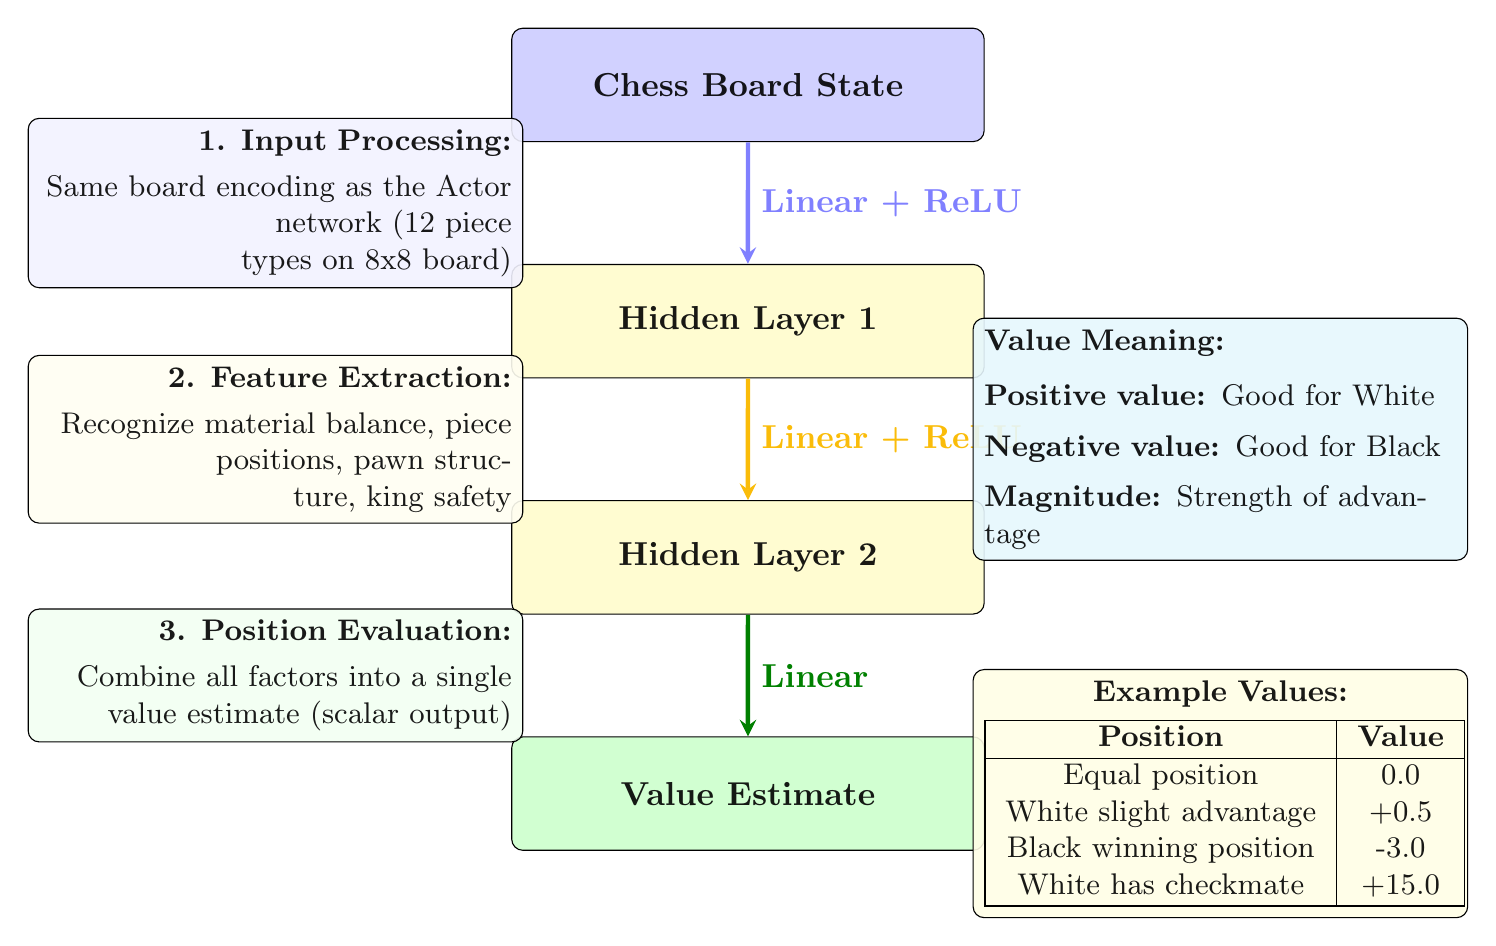
\begin{tikzpicture}[scale=1.2, every node/.style={transform shape}]
        % Create vertical network layout with absolute positioning and increased spacing
        \node[draw, rectangle, fill=blue!20, rounded corners, minimum width=5cm, minimum height=1.2cm, align=center, fill opacity=0.9] (input) at (0,0) {\textbf{Chess Board State}};
        \node[draw, rectangle, fill=yellow!20, rounded corners, minimum width=5cm, minimum height=1.2cm, align=center, fill opacity=0.9] (hidden1) at (0,-2.5) {\textbf{Hidden Layer 1}};
        \node[draw, rectangle, fill=yellow!20, rounded corners, minimum width=5cm, minimum height=1.2cm, align=center, fill opacity=0.9] (hidden2) at (0,-5) {\textbf{Hidden Layer 2}};
        \node[draw, rectangle, fill=green!20, rounded corners, minimum width=5cm, minimum height=1.2cm, align=center, fill opacity=0.9] (output) at (0,-7.5) {\textbf{Value Estimate}};
        
        % Connect nodes with descriptive labels and thicker arrows
        \draw[->, ultra thick, >=stealth, blue!50] (input) -- node[right, align=left, font=\normalsize] {\textbf{Linear + ReLU}} (hidden1);
        \draw[->, ultra thick, >=stealth, yellow!50!orange] (hidden1) -- node[right, align=left, font=\normalsize] {\textbf{Linear + ReLU}} (hidden2);
        \draw[->, ultra thick, >=stealth, green!50!black] (hidden2) -- node[right, align=left, font=\normalsize] {\textbf{Linear}} (output);
        
        % Add processing steps on the left with better spacing
        \node[draw, rounded corners, fill=blue!5, align=right, font=\small, text width=5cm, fill opacity=0.9] at (-5,-1.25) {\textbf{1. Input Processing:}\\[0.1cm]Same board encoding as the Actor\\network (12 piece types on 8x8 board)};
        
        \node[draw, rounded corners, fill=yellow!5, align=right, font=\small, text width=5cm, fill opacity=0.9] at (-5,-3.75) {\textbf{2. Feature Extraction:}\\[0.1cm]Recognize material balance, piece\\positions, pawn structure, king safety};
        
        \node[draw, rounded corners, fill=green!5, align=right, font=\small, text width=5cm, fill opacity=0.9] at (-5,-6.25) {\textbf{3. Position Evaluation:}\\[0.1cm]Combine all factors into a single\\value estimate (scalar output)};
        
        % Add explanation of value on the right with better spacing
        \node[draw, rounded corners, fill=cyan!10, align=left, font=\small, text width=5cm, fill opacity=0.9] at (5,-3.75) {\textbf{Value Meaning:}\\[0.2cm]\textbf{Positive value:} Good for White\\[0.15cm]\textbf{Negative value:} Good for Black\\[0.15cm]\textbf{Magnitude:} Strength of advantage};
        
        % Add example values table
        \node[draw, rounded corners, fill=yellow!10, align=center, font=\small, text width=5cm, fill opacity=0.9] at (5,-7.5) {
            \textbf{Example Values:}\\[0.1cm]
            \begin{tabular}{|c|c|}
                \hline
                \textbf{Position} & \textbf{Value} \\
                \hline
                Equal position & 0.0 \\
                White slight advantage & +0.5 \\
                Black winning position & -3.0 \\
                White has checkmate & +15.0 \\
                \hline
            \end{tabular}
        };
    \end{tikzpicture}
    \caption{Critic Network data flow (vertical layout)}
    \label{fig:critic_flow}
\end{figure}

1. \textbf{Input Processing}: Just like the Actor, the Critic takes the chess board state as input.

2. \textbf{Hidden Layers}: The state passes through multiple hidden layers with ReLU activation functions. Each layer helps the network recognize different patterns that contribute to position evaluation:
   - Material advantage (how many pieces each player has)
   - Piece positions (e.g., knights in the center are better than at the edges)
   - King safety (is the king well protected?)
   - Pawn structure (are pawns well organized or weak?)
   - Control of key squares (especially the center)

3. \textbf{Output Layer}: Unlike the Actor, which outputs probabilities for all possible moves, the Critic outputs just a single number - its estimate of how good the current position is.

\subsubsection*{Concrete Example of Critic Network Evaluation}

Let's look at how the Critic might evaluate different chess positions:

\begin{center}
\begin{tabular}{|p{4cm}|c|p{5cm}|}
\hline
\textbf{Position Description} & \textbf{Value Estimate} & \textbf{Interpretation} \\
\hline
 Starting position & 0.0 & Equal chances for both players \\
\hline
 White up a queen & +9.0 & Strong advantage for White \\
\hline
 Black up a pawn, controls center & -1.5 & Slight advantage for Black \\
\hline
 White has checkmate in 2 & +15.0 & Winning position for White \\
\hline
\end{tabular}
\end{center}

These value estimates are crucial for calculating advantages, which guide the learning process. The advantage (how much better a move is compared to the average) is calculated as the difference between what actually happened and what the Critic predicted would happen.

\subsection{End-to-End Training Process}

\subsubsection{How Everything Works Together}

Now that we understand the chess environment representation, the Actor network, the Critic network, and the PPO algorithm, let's see how all these components work together to train our chess AI.

\begin{figure}[p]
    \centering
    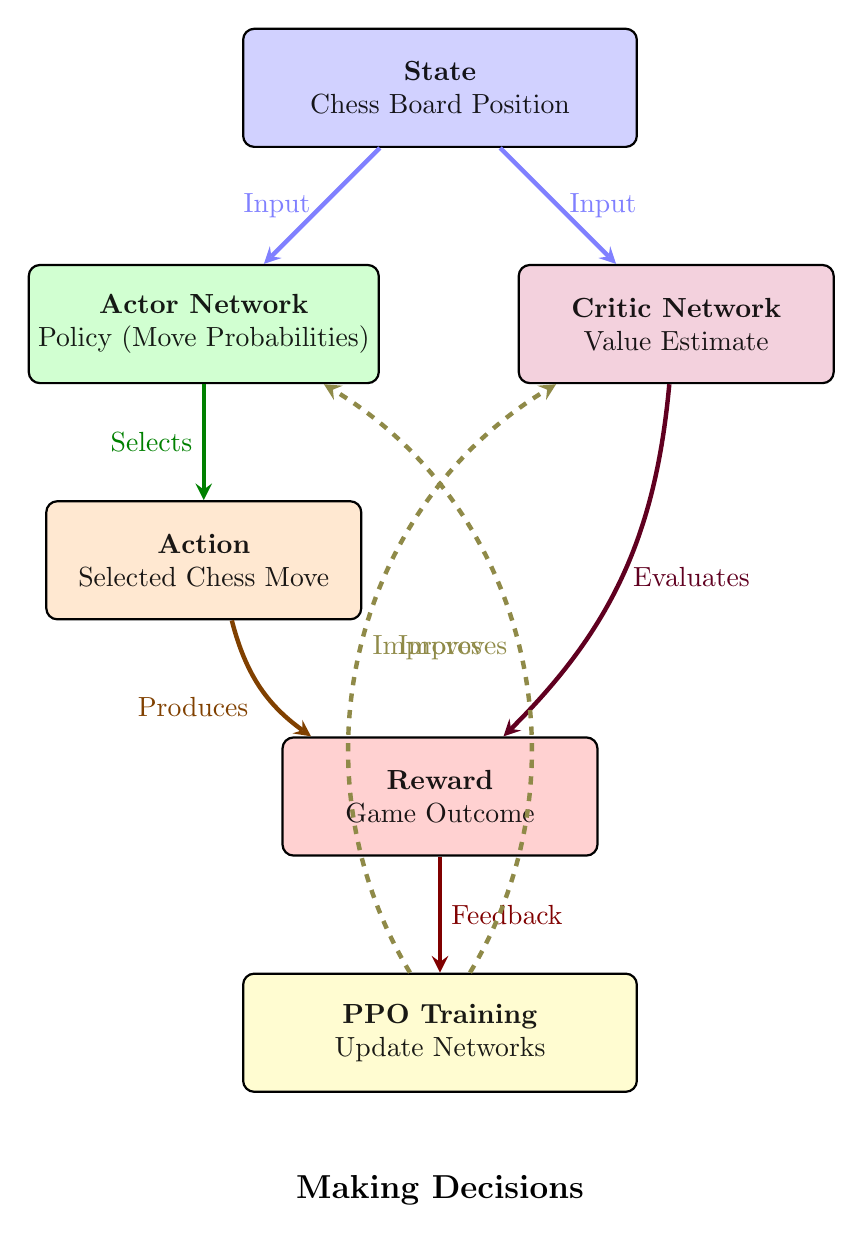
\begin{tikzpicture}[node distance=2.5cm, auto, thick, scale=1.0, transform shape]
        % Define the nodes with improved styling in a vertical layout
        \node[draw, rectangle, fill=blue!20, rounded corners, minimum width=5cm, minimum height=1.5cm, align=center, fill opacity=0.9] (state) at (0,0) {\textbf{State}\\Chess Board Position};
        
        % Actor branch on the left
        \node[draw, rectangle, fill=green!20, rounded corners, minimum width=4cm, minimum height=1.5cm, align=center, fill opacity=0.9] (actor) at (-3,-3) {\textbf{Actor Network}\\Policy (Move Probabilities)};
        
        \node[draw, rectangle, fill=orange!20, rounded corners, minimum width=4cm, minimum height=1.5cm, align=center, fill opacity=0.9] (action) at (-3,-6) {\textbf{Action}\\Selected Chess Move};
        
        % Critic branch on the right
        \node[draw, rectangle, fill=purple!20, rounded corners, minimum width=4cm, minimum height=1.5cm, align=center, fill opacity=0.9] (critic) at (3,-3) {\textbf{Critic Network}\\Value Estimate};
        
        \node[draw, rectangle, fill=red!20, rounded corners, minimum width=4cm, minimum height=1.5cm, align=center, fill opacity=0.9] (reward) at (0,-9) {\textbf{Reward}\\Game Outcome};
        
        \node[draw, rectangle, fill=yellow!20, rounded corners, minimum width=5cm, minimum height=1.5cm, align=center, fill opacity=0.9] (training) at (0,-12) {\textbf{PPO Training}\\Update Networks};
        
        % Connect the nodes with styled arrows
        \draw[->, ultra thick, >=stealth, blue!50] (state) -- node[midway, left, align=right] {Input} (actor);
        \draw[->, ultra thick, >=stealth, blue!50] (state) -- node[midway, right, align=left] {Input} (critic);
        
        \draw[->, ultra thick, >=stealth, green!50!black] (actor) -- node[midway, left, align=right] {Selects} (action);
        
        \draw[->, ultra thick, >=stealth, orange!50!black] (action) to[bend right=20] node[midway, below left, align=right] {Produces} (reward);
        
        \draw[->, ultra thick, >=stealth, purple!50!black] (critic) to[bend left=20] node[midway, right, align=left] {Evaluates} (reward);
        
        \draw[->, ultra thick, >=stealth, red!50!black] (reward) -- node[midway, right, align=left] {Feedback} (training);
        
        \draw[->, ultra thick, >=stealth, yellow!50!black, dashed] (training) to[bend right=45] node[midway, left, align=right] {Improves} (actor);
        
        \draw[->, ultra thick, >=stealth, yellow!50!black, dashed] (training) to[bend left=45] node[midway, right, align=left] {Improves} (critic);
        
        % Add a title
        \node[font=\bfseries\large, text width=5cm, align=center] at (0,-14) {Making Decisions};
    \end{tikzpicture}
    \caption{End-to-End Training System based on the Actor-Critic architecture \cite{mnih2015} and PPO algorithm \cite{schulman2017}}
    \label{fig:end_to_end}
\end{figure}

\begin{figure}[ht]
    \centering
    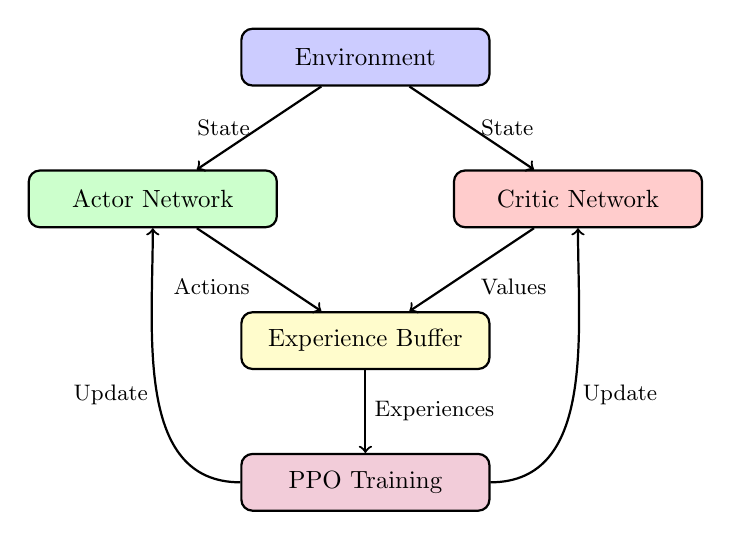
\begin{tikzpicture}[node distance=1.5cm, auto, thick, scale=0.9, transform shape]
        % Define nodes vertically with increased spacing
        \node[draw, rectangle, fill=blue!20, rounded corners, minimum width=3.5cm, minimum height=0.8cm, align=center] (env) at (0,0) {Environment};
        
        \node[draw, rectangle, fill=green!20, rounded corners, minimum width=3.5cm, minimum height=0.8cm, align=center] (actor) at (-3,-2) {Actor Network};
        \node[draw, rectangle, fill=red!20, rounded corners, minimum width=3.5cm, minimum height=0.8cm, align=center] (critic) at (3,-2) {Critic Network};
        
        \node[draw, rectangle, fill=yellow!20, rounded corners, minimum width=3.5cm, minimum height=0.8cm, align=center] (buffer) at (0,-4) {Experience Buffer};
        
        \node[draw, rectangle, fill=purple!20, rounded corners, minimum width=3.5cm, minimum height=0.8cm, align=center] (training) at (0,-6) {PPO Training};
        
        % Connect nodes with labeled edges and better spacing
        \draw[->, thick] (env) -- node[left, font=\small] {State} (actor);
        \draw[->, thick] (env) -- node[right, font=\small] {State} (critic);
        \draw[->, thick] (actor) -- node[below left, font=\small] {Actions} (buffer);
        \draw[->, thick] (critic) -- node[below right, font=\small] {Values} (buffer);
        \draw[->, thick] (buffer) -- node[right, font=\small] {Experiences} (training);
        \draw[->, thick] (training) to[out=180, in=270] node[left, font=\small] {Update} (actor);
        \draw[->, thick] (training) to[out=0, in=270] node[right, font=\small] {Update} (critic);
    \end{tikzpicture}
    \caption{End-to-End Training System (Vertical Layout)}
    \label{fig:training_system}
\end{figure}

\subsection{Training Process in Detail}

Here's how the training process works step by step:

\begin{algorithm}[h]
    \caption{PPO Training Algorithm}
    \begin{algorithmic}[1]
        \For{each episode}
            \State Reset the environment to get initial state $s_0$
            \For{each step $t$ in episode}
                \State Get action $a_t$, log probability $\log \pi_{old}(a_t|s_t)$, and value $V(s_t)$
                \State Execute action $a_t$ in environment
                \State Observe reward $r_t$ and next state $s_{t+1}$
                \State Store $(s_t, a_t, r_t, V(s_t), \log \pi_{old}(a_t|s_t))$ in buffer
            \EndFor
            \State Compute advantage estimates $A_t$ using GAE
            \For{each optimization epoch}
                \For{each mini-batch}
                    \State Compute policy loss $L^{CLIP}$
                    \State Compute value loss $L^{VF}$
                    \State Update actor and critic networks
                \EndFor
            \EndFor
        \EndFor
    \end{algorithmic}
\end{algorithm}

\subsection{Concrete Training Example}

Let's walk through a specific example of a training iteration for better understanding:

\subsubsection*{1. Playing the Game}

Imagine our chess AI is at the beginning of a game:

\begin{itemize}
    \item The board is in the starting position $s_0$
    \item The Actor network looks at the board and outputs move probabilities
    \item The action mask ensures only legal moves are considered
    \item The AI decides to play e2e4 (moving the king's pawn forward two squares)
    \item The Critic network evaluates the new position as $V(s_1) = +0.1$ (slightly better for white)
    \item The environment gives a small reward $r_0 = 0.01$ for controlling the center
\end{itemize}

This process continues for many moves until the game ends (either in checkmate, stalemate, or after a maximum number of moves).

\subsubsection*{2. Learning from Experience}

After playing multiple games and collecting experiences, the learning begins:

\textbf{Advantage Calculation Example:}
\begin{itemize}
    \item For a move that led to capturing the opponent's queen, the real outcome was much better than the Critic predicted
    \item Say the Critic predicted $V(s_t) = +2.0$, but after capturing the queen and seeing subsequent positions, the actual return was $+11.0$
    \item The advantage would be $A_t = +11.0 - (+2.0) = +9.0$, indicating this move was much better than expected
\end{itemize}

\textbf{Network Update Example:}
Using the calculated advantages, we update both networks:

\begin{itemize}
    \item For moves with high advantages (like capturing the queen), the policy is adjusted to make these moves more likely in similar positions
    \item For moves with negative advantages (like blunders), the policy is adjusted to make these moves less likely
    \item The Critic network is updated to make more accurate predictions about position values
\end{itemize}

\subsection{Multi-Agent Learning}

One of the most powerful aspects of our system is multi-agent learning. Rather than training against a static opponent, our agents play against each other and learn from these interactions:

\begin{itemize}
    \item Multiple AI agents with different parameters play against each other
    \item Each agent learns from its games and improves over time
    \item As one agent gets better, it provides stronger opposition for the others
    \item This creates a self-improving cycle where the competition drives improvement
\end{itemize}

This is similar to how human chess players improve by playing against stronger opponents.

\subsection{From Beginner to Master: The Learning Journey}

Through thousands of games of self-play, our AI progresses through distinct stages of chess understanding:

\begin{enumerate}
    \item \textbf{Beginner Stage}: The AI learns basic rules and avoids obvious blunders
    \item \textbf{Intermediate Stage}: The AI begins to understand positional concepts like center control and piece development
    \item \textbf{Advanced Stage}: The AI learns complex strategies, sacrifices, and long-term planning
    \item \textbf{Master Stage}: The AI develops sophisticated pattern recognition and intuition for chess positions
\end{enumerate}

Just like a human player, the AI doesn't need to be explicitly taught these concepts - it discovers them through experimentation and learning from outcomes.

\subsection{Why This Approach Works}

Our multi-agent deep reinforcement learning approach to chess has several key advantages:

\begin{itemize}
    \item \textbf{No Human Bias}: Unlike traditional chess engines that use human-designed evaluation functions, our AI develops its own understanding of chess
    \item \textbf{Continuous Improvement}: Through self-play, the system continues to improve without needing new training data
    \item \textbf{Creativity}: Because it isn't limited by human preconceptions, the AI sometimes finds unusual but effective moves
    \item \textbf{Adaptability}: The same approach can be applied to other chess variants or even different games entirely
\end{itemize}

This represents a fundamental shift in how we approach AI for strategic games - from explicitly programming knowledge to creating systems that can learn and discover strategies on their own.

\section{Super Simple Step-by-Step Implementation Guide}

\subsection{Getting Started: Setting Up Your First Chess AI}

Let's break down how to build our chess AI into tiny steps that anyone can follow! Think of this like building with LEGO blocks - we'll put one piece at a time until we have our complete chess robot!

\begin{tcolorbox}[colback=blue!5!white,colframe=blue!75!black,title=Computer Setup Steps]
\begin{enumerate}
    \item Install Python on your computer (it's a language that helps us talk to computers)
    \item Install these special Python packages:
    \begin{itemize}
        \item PyTorch (for building our robot brain)
        \item python-chess (for understanding chess rules)
        \item numpy (for math calculations)
        \item matplotlib (for making pictures of our results)
    \end{itemize}
    \item Create a new folder on your computer called "ChessAI"
    \item Inside this folder, create these sub-folders:
    \begin{itemize}
        \item chess (for chess rules)
        \item agents (for our robot players)
        \item buffer (for memory storage)
        \item learnings (for the learning algorithm)
    \end{itemize}
\end{enumerate}
\end{tcolorbox}

\subsection{Step 1: Building Our Chess World}

First, we need to create a world where our AI can play chess. Think of this like building a chess board and teaching the computer the rules.

\begin{tcolorbox}[colback=green!5!white,colframe=green!75!black,title=Creating the Chess Environment]
\textbf{File: chess/chess.py}
\begin{lstlisting}[style=Python]
import numpy as np
import chess

class ChessEnv:
    def __init__(self):
        # This creates a brand new chess board with all pieces in starting positions
        self.board = chess.Board()
        # This keeps track of whose turn it is (White=0, Black=1)
        self.turn = 0
        
    def reset(self):
        # Reset the board to starting position
        self.board = chess.Board()
        self.turn = 0
        # Return the current state (how the board looks)
        return self.get_state()
        
    def get_state(self):
        # Turn the chess board into numbers that our AI can understand
        # We'll use a 8x8x12 representation (8x8 board, 12 piece types)
        state = np.zeros((12, 8, 8), dtype=np.float32)
        
        # Go through each square on the board
        for i in range(64):
            # Convert to row and column (0-7 for each)
            row = i // 8
            col = i % 8
            # Get the piece at this square
            piece = self.board.piece_at(i)
            
            if piece:
                # Figure out piece type (0-5) and color
                piece_type = piece.piece_type - 1  # 0-5 for each piece type
                color = 0 if piece.color else 6  # White=0, Black=6
                # Mark this piece's position in our state array
                state[piece_type + color, row, col] = 1.0
                
        return state
    
    def get_legal_moves(self):
        # Create a mask of legal moves (1 for legal, 0 for illegal)
        mask = np.zeros(4096, dtype=np.float32)
        
        # For each legal move
        for move in self.board.legal_moves:
            # Convert the move to a number between 0-4095
            move_idx = self.move_to_index(move)
            # Mark this move as legal
            mask[move_idx] = 1.0
            
        return mask
    
    def move_to_index(self, move):
        # Convert chess move to a number between 0-4095
        from_square = move.from_square  # 0-63
        to_square = move.to_square  # 0-63
        # Combine these into a single number
        return from_square * 64 + to_square
    
    def index_to_move(self, idx):
        # Convert our number back to a chess move
        from_square = idx // 64
        to_square = idx % 64
        return chess.Move(from_square, to_square)
    
    def step(self, action):
        # Take an action (make a move)
        # Action is a number 0-4095
        
        # Convert action to a chess move
        move = self.index_to_move(action)
        
        # Make sure it's a legal move
        if move in self.board.legal_moves:
            # Make the move
            self.board.push(move)
            # Switch turns
            self.turn = 1 - self.turn
            
            # Check if the game is over
            done = self.board.is_game_over()
            
            # Calculate reward
            reward = 0
            if done:
                if self.board.is_checkmate():
                    # Big reward for checkmate
                    reward = 1.0 if self.turn == 1 else -1.0
                    
            # Return the new state, reward, and whether game is done
            return self.get_state(), reward, done
        else:
            # Illegal move - big penalty!
            return self.get_state(), -1.0, True

    def render(self):
        # Print the board so humans can see it
        print(self.board)
\end{lstlisting}
\end{tcolorbox}

\subsection{Let's Understand Our Chess World}

Imagine we've built a magical chess board that a computer can understand. Let's see how it works with a simple example:

\begin{tcolorbox}[colback=yellow!5!white,colframe=yellow!75!black,title=Example: Setting Up and Making a Move]
\begin{lstlisting}[style=Python]
# Create our chess world
chess_env = ChessEnv()

# Start a new game
state = chess_env.reset()

# Show the board
chess_env.render()
# This would print:
# r n b q k b n r
# p p p p p p p p
# . . . . . . . .
# . . . . . . . .
# . . . . . . . .
# . . . . . . . .
# P P P P P P P P
# R N B Q K B N R

# See what moves are legal
legal_moves = chess_env.get_legal_moves()
# This would show a big array with 1s for legal moves

# Let's make a move (e2e4 - moving pawn two squares forward)
# The index for e2e4 is 52*64 + 36 = 3368
new_state, reward, done = chess_env.step(3368)

# Show the board after move
chess_env.render()
# This would print:
# r n b q k b n r
# p p p p p p p p
# . . . . . . . .
# . . . . . . . .
# . . . . P . . .
# . . . . . . . .
# P P P P . P P P
# R N B Q K B N R
\end{lstlisting}
\end{tcolorbox}

Now we've built a world where our AI can play chess! The computer understands:
\begin{itemize}
    \item What the board looks like (\texttt{get\_state()})
    \item What moves are allowed (\texttt{get\_legal\_moves()})
    \item How to make moves (\texttt{step()})
    \item When someone has won (\texttt{step()} returns \texttt{done=True})
\end{itemize}

\subsection{Step 2: Building Our Robot Brain (Neural Networks)}

Now we need to build the brain for our chess robot! We'll make two parts for the brain:
\begin{enumerate}
    \item The "Actor" part: This decides which chess move to make
    \item The "Critic" part: This tells us how good our current position is
\end{enumerate}

Let's start with the Actor - the part that decides which move to make:

\begin{tcolorbox}[colback=purple!5!white,colframe=purple!75!black,title=Building the Actor Network]
\textbf{File: learnings/ppo/actor.py}
\begin{minipage}[t]{0.48\textwidth}
\begin{lstlisting}[style=Python]
import torch as T
import torch.nn as nn
import torch.nn.functional as F
from torch.distributions import Categorical

class Actor(nn.Module):
    def __init__(self, state_dim, action_dim, 
                 hidden_layers):
        super().__init__()
        
        # Create parts of our robot brain
        layers = []
        prev_dim = state_dim  # Input size
        
        # Add hidden layers (help brain think)
        for dim in hidden_layers:
            # Layer to recognize patterns
            layers.append(nn.Linear(prev_dim, dim))
            # Special sauce for learning
            layers.append(nn.ReLU())
            # Update for next layer
            prev_dim = dim
        
        # Final layer for move decisions
        layers.append(nn.Linear(prev_dim, 
                               action_dim))
        # Turn numbers into probabilities
        layers.append(nn.Softmax(dim=-1))
        
        # Combine into one brain
        self.model = nn.Sequential(*layers)
\end{lstlisting}
\end{minipage}\hfill
\begin{minipage}[t]{0.48\textwidth}
\begin{lstlisting}[style=Python]
    def forward(self, state, action_mask):
        # Look at board and decide move
        # action_mask shows legal moves
        
        # Get move probabilities
        probs = self.model(state)
        
        # Only consider legal moves
        probs = probs * action_mask
        
        # Normalize probabilities
        probs = probs / probs.sum(dim=1, 
                                keepdim=True)
        
        # Create probability distribution
        dist = Categorical(probs)
        
        return dist
    
    def log_prob(self, state, action):
        # Calculate move likelihood
        # Helps learn if it was good
        
        # Get move probabilities
        probs = self.model(state)
        
        # Create probability distribution
        dist = Categorical(probs)
        
        # Get log probability of action
        return dist.log_prob(action)
\end{lstlisting}
\end{minipage}
\end{tcolorbox}

Now let's build the Critic - the part that tells us how good our position is:

\begin{tcolorbox}[colback=red!5!white,colframe=red!75!black,title=Building the Critic Network]
\textbf{File: learnings/ppo/critic.py}
\begin{lstlisting}[style=Python]
import torch as T
import torch.nn as nn
import torch.nn.functional as F

class Critic(nn.Module):
    def __init__(self, state_dim, hidden_layers):
        super().__init__()
        
        # Create all the parts of our rating brain
        layers = []
        prev_dim = state_dim  # Start with input size
        
        # Add hidden layers (these help the brain think)
        for dim in hidden_layers:
            # Add a layer that can recognize patterns
            layers.append(nn.Linear(prev_dim, dim))
            # Add special sauce that helps the robot learn
            layers.append(nn.ReLU())
            # Update for next layer
            prev_dim = dim
        
        # Add final layer that gives a single score
        layers.append(nn.Linear(prev_dim, 1))
        
        # Put all the layers together into one brain
        self.model = nn.Sequential(*layers)
    
    def forward(self, state):
        # Look at the chess board and decide how good our position is
        # Returns a single number: higher = better for us
        return self.model(state)
\end{lstlisting}
\end{tcolorbox}

\subsection{Understanding Our Robot Brain with Simple Examples}

Let's see how our robot brain works with a simple example. Imagine we have a chess board and want to decide what move to make:

\begin{tcolorbox}[colback=orange!5!white,colframe=orange!75!black,title=Example: How Our Robot Makes Decisions, width=\textwidth]
\begin{lstlisting}[style=Python, basicstyle=\ttfamily\small]
# Create our chess world
chess_env = ChessEnv()
state = chess_env.reset()

# Create our robot brain (with simple settings)
state_dim = 12 * 8 * 8    # 12 piece types, 8x8 board
action_dim = 4096         # 64 starting squares x 64 ending squares
hidden_layers = (256, 256) # Two thinking layers

# Create actor and critic
actor = Actor(state_dim, action_dim, hidden_layers)
critic = Critic(state_dim, hidden_layers)

# Flatten the state to feed into our networks
flat_state = T.FloatTensor(state).reshape(1, -1)

# Get legal moves
action_mask = T.FloatTensor(chess_env.get_legal_moves())

# Ask actor which move to make
dist = actor(flat_state, action_mask)

# Sample a move (let's say it chose e2e4)
action = dist.sample()    # This might give us 3368

# Ask critic how good our position is
value = critic(flat_state) # Might give us 0.1

# Make the move
new_state, reward, done = chess_env.step(action.item())
# This is one step of playing! Our robot has made a move.
\end{lstlisting}
\end{tcolorbox}

\begin{figure}[ht]
    \centering
    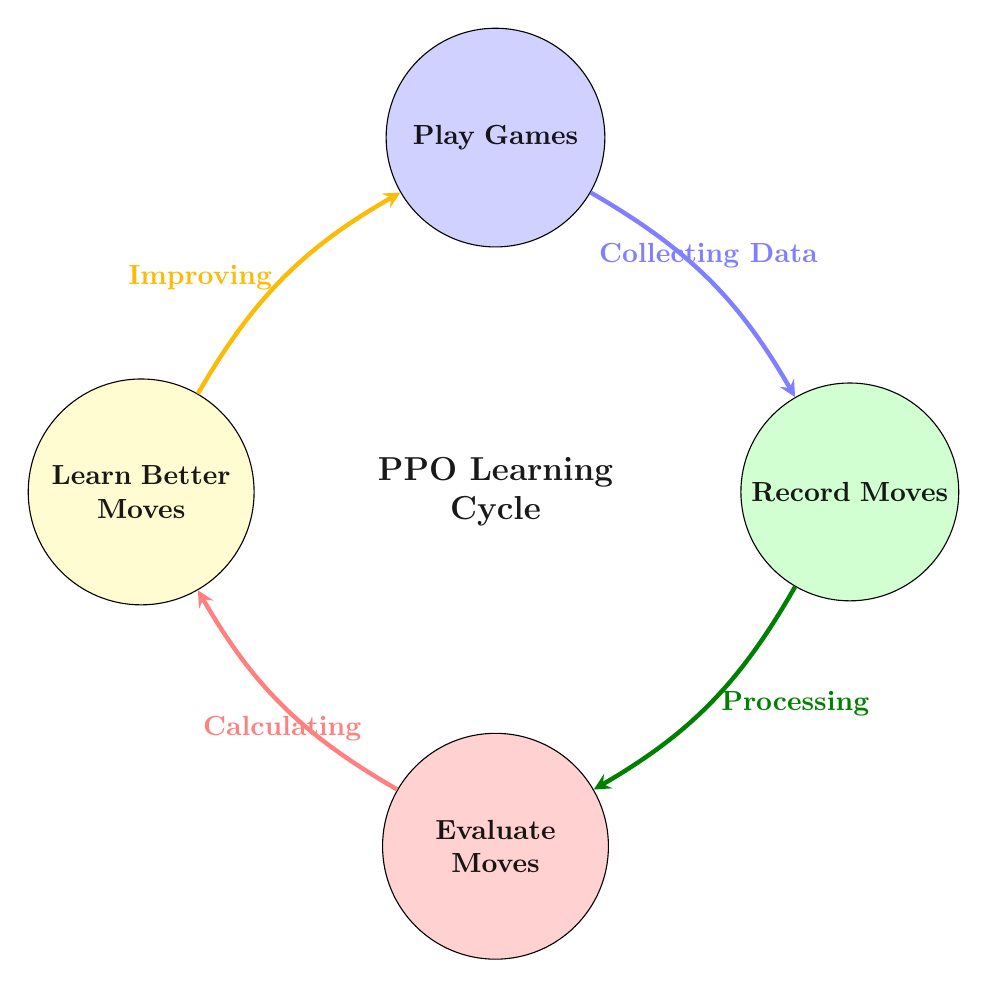
\begin{tikzpicture}[node distance=3cm, auto, scale=1.0, transform shape]
        % Define circle radius and positions
        \def\radius{4.5cm}
        \def\noderad{1.5cm}
        
        % Create nodes in a circular arrangement
        \node[circle, draw, fill=blue!20, rounded corners, minimum size=\noderad, text width=2.5cm, align=center, fill opacity=0.9] (play) at (90:\radius) {\textbf{Play Games}};
        
        \node[circle, draw, fill=green!20, rounded corners, minimum size=\noderad, text width=2.5cm, align=center, fill opacity=0.9] (record) at (0:\radius) {\textbf{Record Moves}};
        
        \node[circle, draw, fill=red!20, rounded corners, minimum size=\noderad, text width=2.5cm, align=center, fill opacity=0.9] (analyze) at (270:\radius) {\textbf{Evaluate Moves}};
        
        \node[circle, draw, fill=yellow!20, rounded corners, minimum size=\noderad, text width=2.5cm, align=center, fill opacity=0.9] (learn) at (180:\radius) {\textbf{Learn Better Moves}};
        
        % Connect nodes with curved arrows and better labels
        \draw[->, ultra thick, >=stealth, blue!50, bend left=15] (play) to node[midway, above, font=\normalsize] {\textbf{Collecting Data}} (record);
        
        \draw[->, ultra thick, >=stealth, green!50!black, bend left=15] (record) to node[midway, right, font=\normalsize] {\textbf{Processing}} (analyze);
        
        \draw[->, ultra thick, >=stealth, red!50, bend left=15] (analyze) to node[midway, below, font=\normalsize] {\textbf{Calculating}} (learn);
        
        \draw[->, ultra thick, >=stealth, yellow!50!orange, bend left=15] (learn) to node[midway, left, font=\normalsize] {\textbf{Improving}} (play);
        
        % Add a title in the center of the circle
        \node[font=\bfseries\large, text width=3cm, align=center, fill=white, rounded corners, fill opacity=0.9] at (0,0) {PPO Learning Cycle};
    \end{tikzpicture}
    \caption{The PPO learning cycle showing how the AI continuously improves through gameplay and feedback}
    \label{fig:ppo_learning_cycle}
\end{figure}

\begin{figure}[ht]
    \centering
    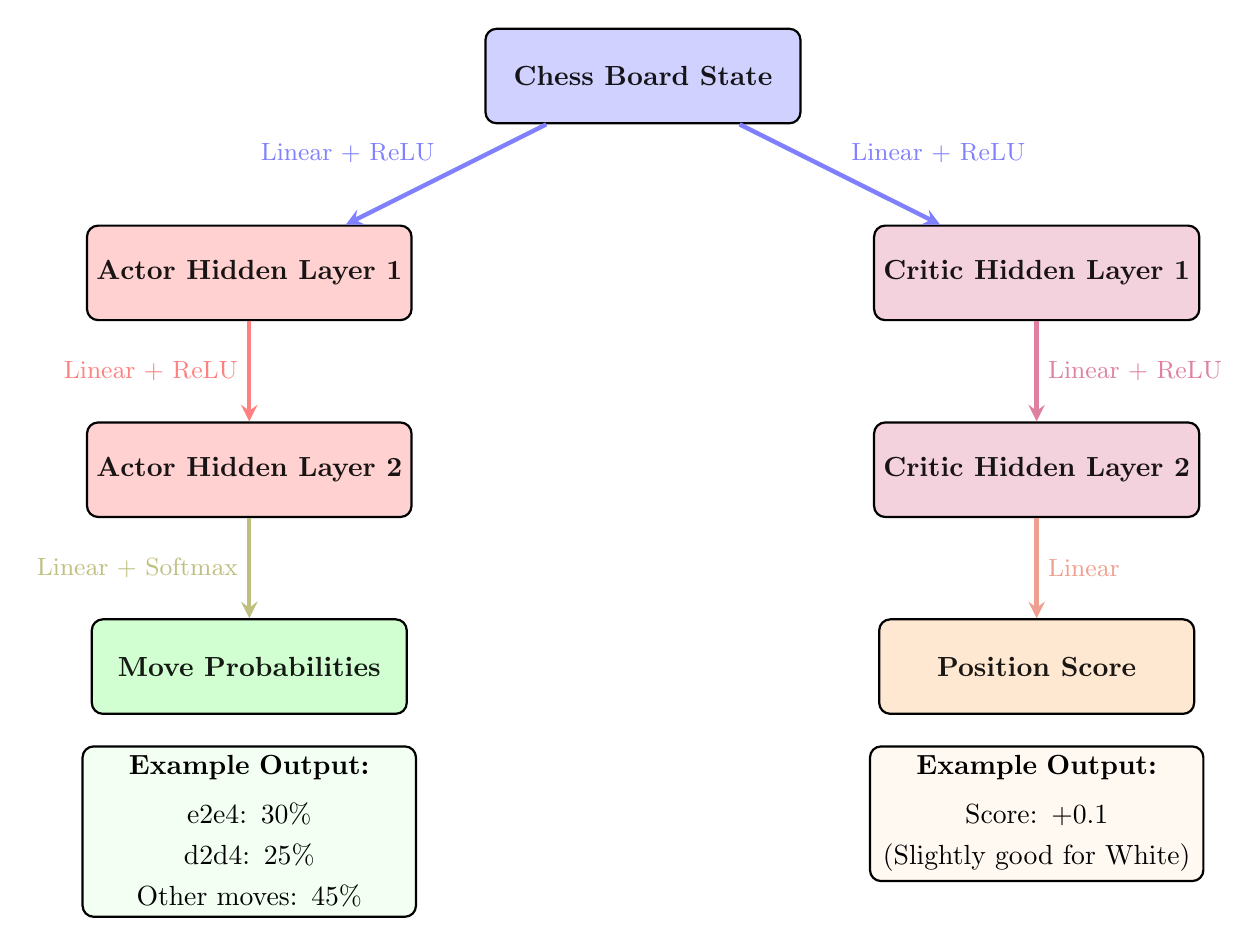
\begin{tikzpicture}[node distance=3cm, auto, thick, scale=1.0, transform shape]
        % Nodes with better spacing and design
        \node[draw, rectangle, fill=blue!20, rounded corners, minimum width=4cm, minimum height=1.2cm, align=center, fill opacity=0.9] (input) at (0,0) {\textbf{Chess Board State}};
        
        \node[draw, rectangle, fill=red!20, rounded corners, minimum width=4cm, minimum height=1.2cm, align=center, fill opacity=0.9] (actor1) at (-5,-2.5) {\textbf{Actor Hidden Layer 1}};
        \node[draw, rectangle, fill=red!20, rounded corners, minimum width=4cm, minimum height=1.2cm, align=center, fill opacity=0.9] (actor2) at (-5,-5) {\textbf{Actor Hidden Layer 2}};
        \node[draw, rectangle, fill=green!20, rounded corners, minimum width=4cm, minimum height=1.2cm, align=center, fill opacity=0.9] (output1) at (-5,-7.5) {\textbf{Move Probabilities}};
        
        \node[draw, rectangle, fill=purple!20, rounded corners, minimum width=4cm, minimum height=1.2cm, align=center, fill opacity=0.9] (critic1) at (5,-2.5) {\textbf{Critic Hidden Layer 1}};
        \node[draw, rectangle, fill=purple!20, rounded corners, minimum width=4cm, minimum height=1.2cm, align=center, fill opacity=0.9] (critic2) at (5,-5) {\textbf{Critic Hidden Layer 2}};
        \node[draw, rectangle, fill=orange!20, rounded corners, minimum width=4cm, minimum height=1.2cm, align=center, fill opacity=0.9] (output2) at (5,-7.5) {\textbf{Position Score}};
        
        % Connections with better visibility
        \draw[->, ultra thick, >=stealth, blue!50] (input) -- node[above left, font=\small] {Linear + ReLU} (actor1);
        \draw[->, ultra thick, >=stealth, red!50] (actor1) -- node[left, font=\small] {Linear + ReLU} (actor2);
        \draw[->, ultra thick, >=stealth, red!50!green!50] (actor2) -- node[left, font=\small] {Linear + Softmax} (output1);
        
        \draw[->, ultra thick, >=stealth, blue!50] (input) -- node[above right, font=\small] {Linear + ReLU} (critic1);
        \draw[->, ultra thick, >=stealth, purple!50] (critic1) -- node[right, font=\small] {Linear + ReLU} (critic2);
        \draw[->, ultra thick, >=stealth, purple!50!orange!50] (critic2) -- node[right, font=\small] {Linear} (output2);
        
        % Example outputs with better spacing
        \node[draw, fill=green!5, rounded corners, text width=4cm, align=center, below=1cm] (output1_text) at (-5,-7.5) {\textbf{Example Output:}\\[0.2cm]e2e4: 30\%\\[0.1cm]d2d4: 25\%\\[0.1cm]Other moves: 45\%};
        \node[draw, fill=orange!5, rounded corners, text width=4cm, align=center, below=1cm] (output2_text) at (5,-7.5) {\textbf{Example Output:}\\[0.2cm]Score: +0.1\\[0.1cm](Slightly good for White)};
    \end{tikzpicture}
    \caption{How our robot brain works - simple explanation}
    \label{fig:robot_brain}
\end{figure}

\subsection{Step 3: Teaching Our Robot to Learn (PPO Algorithm)}

Now we need to teach our robot how to learn from its mistakes and get better at chess. We'll use something called PPO (Proximal Policy Optimization) - think of it like special training exercises for our robot.

\begin{tcolorbox}[colback=cyan!5!white,colframe=cyan!75!black,title=Building the PPO Learning System,width=\textwidth]
\textbf{File: learnings/ppo/ppo.py}
% Using minipage instead of multicols for better compatibility
\begin{minipage}{0.48\textwidth}
\begin{lstlisting}[style=Python,basicstyle=\ttfamily\scriptsize]
import torch as T
import torch.optim as optim
import numpy as np
from tqdm import tqdm

from learnings.base import Learning
from learnings.ppo.actor import Actor
from learnings.ppo.critic import Critic
from buffer.ppo import BufferPPO

class PPO(Learning):
    def __init__(
        self,
        environment,  # Our chess world
        hidden_layers,  # How many neurons
        epochs,  # Learning repetitions
        buffer_size,  # Memory size
        batch_size,  # Batch size
        gamma=0.99,  # Future reward factor
        gae_lambda=0.95,  # Learning parameter
        policy_clip=0.2,  # Change limit
        learning_rate=0.003,  # Learn speed
    ):
        super().__init__(environment, 
                       epochs, gamma, 
                       learning_rate)
        
        # Save all our settings
        self.gae_lambda = gae_lambda
        self.policy_clip = policy_clip
        
        # Create our memory (experiences)
        self.buffer = BufferPPO(
            gamma=gamma,
            max_size=buffer_size,
            batch_size=batch_size,
            gae_lambda=gae_lambda,
        )
        
        # Get the sizes for our networks
        self.state_dim = environment.observation_space.shape[0]
        self.action_dim = environment.action_space.n
        
        # Create our actor and critic networks
        self.actor = Actor(self.state_dim, 
                          self.action_dim, 
                          hidden_layers)
        self.critic = Critic(self.state_dim, 
                            hidden_layers)
        
        # Create optimizers for our networks
        self.actor_optimizer = optim.Adam(
            self.actor.parameters(), 
            lr=learning_rate)
        self.critic_optimizer = optim.Adam(
            self.critic.parameters(), 
            lr=learning_rate)
        # Check if we can use a GPU for faster learning
        self.device = T.device('cuda:0' if T.cuda.is_available() else 'cpu')
        self.to(self.device)  # Move our networks to the GPU if available
    
    def to(self, device):
        # Move our networks to the specified device (CPU or GPU)
        self.actor = self.actor.to(device)
        self.critic = self.critic.to(device)
        return self
    
    def take_action(self, state, action_mask):
        # Convert numpy arrays to PyTorch tensors
        state = T.Tensor(state).unsqueeze(0).to(self.device)
        action_mask = T.Tensor(action_mask).unsqueeze(0).to(self.device)
        
        # Ask actor which move to make
        dist = self.actor(state, action_mask)
        action = dist.sample()
        
        # Get probability of chosen move and value estimate
        probs = T.squeeze(dist.log_prob(action)).item()
        value = T.squeeze(self.critic(state)).item()
        action = T.squeeze(action).item()
        
        return action, probs, value
    
    def learn(self):
        # This is the main learning function
        for epoch in tqdm(range(self.epochs), desc="Learning Chess..."):
            self.train_networks()
        self.buffer.clear()  # Clear our memory after learning
    
    def train_networks(self):
        # Get all our experiences from memory
        states, actions, old_probs, values, rewards, advantages, masks = self.buffer.sample()
        
        # Convert everything to PyTorch tensors
        states = T.Tensor(states).to(self.device)
        actions = T.Tensor(actions).to(self.device)
        old_probs = T.Tensor(old_probs).to(self.device)
        advantages = T.Tensor(advantages).to(self.device)
        values = T.Tensor(values).to(self.device)
        masks = T.Tensor(masks).to(self.device)
        
        # Get new action probabilities from our actor
        dist = self.actor(states, masks)
        new_probs = dist.log_prob(actions)
        
        # Calculate probability ratio (new policy / old policy)
        prob_ratio = (new_probs - old_probs).exp()
        
        # Calculate actor loss using PPO clipping
        weighted_probs = advantages * prob_ratio
        weighted_clipped_probs = advantages * T.clamp(prob_ratio, 1-self.policy_clip, 1+self.policy_clip)
        actor_loss = -T.min(weighted_probs, weighted_clipped_probs).mean()
        
        # Calculate critic loss (how wrong our value estimates were)
        critic_value = self.critic(states).squeeze()
        critic_loss = ((critic_value - values)**2).mean()
        
        # Combine losses
        total_loss = actor_loss + 0.5 * critic_loss
        
        # Update both networks
        self.actor_optimizer.zero_grad()
        self.critic_optimizer.zero_grad()
        total_loss.backward()
        self.actor_optimizer.step()
        self.critic_optimizer.step()
\end{lstlisting}
\end{minipage}
\end{tcolorbox}

\subsection{Step 4: Memory - Storing Experiences}

Our robot needs to remember what happened in its games so it can learn from them. Let's build a memory system:

\begin{tcolorbox}[colback=brown!5!white,colframe=brown!75!black,title=Building the Memory System]
\textbf{File: buffer/ppo/module.py}
\begin{lstlisting}[style=Python]
import numpy as np
from collections import deque

class BufferPPO:
    def __init__(self, max_size, batch_size, gamma, gae_lambda):
        # Settings
        self.max_size = max_size  # How many games to remember
        self.batch_size = batch_size  # How many experiences to learn from at once
        self.gamma = gamma  # How much to care about future rewards
        self.gae_lambda = gae_lambda  # Special learning parameter
        
        # Initialize memory containers
        self.states = deque(maxlen=max_size)  # Board positions
        self.actions = deque(maxlen=max_size)  # Moves made
        self.probs = deque(maxlen=max_size)  # Probabilities of moves
        self.values = deque(maxlen=max_size)  # Value estimates
        self.rewards = deque(maxlen=max_size)  # Rewards received
        self.dones = deque(maxlen=max_size)  # Whether game ended
        self.masks = deque(maxlen=max_size)  # Legal move masks
    
    def store(self, state, action, prob, value, reward, done, mask):
        # Store one step of experience
        self.states.append(state)
        self.actions.append(action)
        self.probs.append(prob)
        self.values.append(value)
        self.rewards.append(reward)
        self.dones.append(done)
        self.masks.append(mask)
    
    def clear(self):
        # Clear all memories
        self.states.clear()
        self.actions.clear()
        self.probs.clear()
        self.values.clear()
        self.rewards.clear()
        self.dones.clear()
        self.masks.clear()
    
    def calculate_advantages(self):
        # Calculate advantage estimates for all stored experiences
        advantages = np.zeros(len(self.rewards), dtype=np.float32)
        last_advantage = 0
        last_value = 0
        
        # Work backwards from the end
        for t in reversed(range(len(self.rewards))):
            # If this was the last step in an episode, reset values
            if self.dones[t]:
                last_advantage = 0
                last_value = 0
            
            # Calculate TD error: reward + next_value - current_value
            delta = self.rewards[t] + self.gamma * last_value * (1 - self.dones[t]) - self.values[t]
            
            # Calculate advantage using GAE
            advantages[t] = delta + self.gamma * self.gae_lambda * last_advantage * (1 - self.dones[t])
            
            # Update for next iteration
            last_advantage = advantages[t]
            last_value = self.values[t]
        
        return advantages
    
    def sample(self):
        # Calculate advantages
        advantages = self.calculate_advantages()
        
        # Convert everything to numpy arrays
        states = np.array(self.states)
        actions = np.array(self.actions)
        probs = np.array(self.probs)
        values = np.array(self.values)
        rewards = np.array(self.rewards)
        masks = np.array(self.masks)
        
        return states, actions, probs, values, rewards, advantages, masks
\end{lstlisting}
\end{tcolorbox}

\subsection{Step 5: Putting It All Together - Training Our Chess AI!}

Now let's put all the pieces together to train our chess AI! This is the exciting part where our robot starts learning and getting better at playing chess.

\begin{tcolorbox}[colback=green!10!white,colframe=green!75!black,title=Complete Training Script,width=\textwidth]
\textbf{File: train.py}
% Using minipage instead of multicols for better compatibility
\begin{minipage}{0.48\textwidth}
\begin{lstlisting}[style=Python,basicstyle=\ttfamily\scriptsize]
import torch as T
import numpy as np
import matplotlib.pyplot as plt
import gymnasium as gym
from tqdm import tqdm

from chess.chess import ChessEnv
from learnings.ppo.ppo import PPO

# Create two chess environments (one for each player)
env_white = ChessEnv()
env_black = ChessEnv()

# Set up our PPO learning settings
hidden_layers = (256, 256)  # Two thinking layers with 256 neurons each
epochs = 10  # How many times to learn from each batch of experiences
buffer_size = 2000  # How many steps to remember
batch_size = 64  # How many steps to learn from at once
gamma = 0.99  # How much to care about future rewards
gae_lambda = 0.95  # Special learning parameter
policy_clip = 0.2  # How much to change at once
learning_rate = 0.0003  # How fast to learn

# Create our two AI players
white_player = PPO(
    environment=env_white,
    hidden_layers=hidden_layers,
    epochs=epochs,
    buffer_size=buffer_size,
    batch_size=batch_size,
    gamma=gamma,
    gae_lambda=gae_lambda,
    policy_clip=policy_clip,
    learning_rate=learning_rate,
)

black_player = PPO(
    environment=env_black,
    hidden_layers=hidden_layers,
    epochs=epochs,
    buffer_size=buffer_size,
    batch_size=batch_size,
    gamma=gamma,
    gae_lambda=gae_lambda,
    policy_clip=policy_clip,
    learning_rate=learning_rate,
)

# Keep track of how our players are doing
white_wins = []
black_wins = []
draws = []

# Train for many games
num_games = 1000

print("Starting training for", num_games, "games...")
for game in tqdm(range(num_games)):
    # Reset both environments
    white_state = env_white.reset()
    black_state = env_black.reset()
    
    done = False
    white_turn = True
    
    # Keep track of all experiences in this game
    white_experiences = []
    black_experiences = []
    
    # Play a full game
    while not done:
        if white_turn:
            # White's turn
            # Get legal moves
            action_mask = env_white.get_legal_moves()
            
            # Let white player decide on a move
            action, prob, value = white_player.take_action(white_state, action_mask)
            
            # Make the move in both environments
            next_state, reward, done = env_white.step(action)
            _, _, _ = env_black.step(action)  # Same move in black's environment
            
            # Store experience
            white_experiences.append((white_state, action, prob, value, reward, done, action_mask))
            
            # Update state
            white_state = next_state
        else:
            # Black's turn
            # Get legal moves
            action_mask = env_black.get_legal_moves()
            
            # Let black player decide on a move
            action, prob, value = black_player.take_action(black_state, action_mask)
            
            # Make the move in both environments
            next_state, reward, done = env_black.step(action)
            _, _, _ = env_white.step(action)  # Same move in white's environment
            
            # Store experience
            black_experiences.append((black_state, action, prob, value, reward, done, action_mask))
            
            # Update state
            black_state = next_state
        
        # Switch turns
        white_turn = not white_turn
    
    # After the game is over, store all experiences
    for exp in white_experiences:
        state, action, prob, value, reward, done, mask = exp
        white_player.buffer.store(state, action, prob, value, reward, done, mask)
    
    for exp in black_experiences:
        state, action, prob, value, reward, done, mask = exp
        black_player.buffer.store(state, action, prob, value, reward, done, mask)
    
    # Figure out who won
    if white_experiences[-1][4] > 0:  # Check the reward of white's last move
        white_wins.append(1)
        black_wins.append(0)
        draws.append(0)
    elif black_experiences[-1][4] > 0:  # Check the reward of black's last move
        white_wins.append(0)
        black_wins.append(1)
        draws.append(0)
    else:
        white_wins.append(0)
        black_wins.append(0)
        draws.append(1)
    
    # Learn from experiences every 10 games
    if (game + 1) % 10 == 0:
        white_player.learn()
        black_player.learn()

# After training, save our trained models
T.save(white_player.state_dict(), "white_player.pt")
T.save(black_player.state_dict(), "black_player.pt")

# Plot results to see how our AIs improved
plt.figure(figsize=(10, 6))
plt.plot(np.convolve(white_wins, np.ones(20)/20, mode='valid'), label='White Wins')
plt.plot(np.convolve(black_wins, np.ones(20)/20, mode='valid'), label='Black Wins')
plt.plot(np.convolve(draws, np.ones(20)/20, mode='valid'), label='Draws')
plt.xlabel('Games')
plt.ylabel('Win Rate (20-game moving average)')
plt.title('Chess AI Learning Progress')
plt.legend()
plt.grid(True)
plt.savefig('learning_progress.png')
plt.show()

print("Training complete! Models saved as white_player.pt and black_player.pt")
\end{lstlisting}
\end{minipage}
\end{tcolorbox}

\subsection{What's Happening During Training?}

Let's break down what happens when we train our chess AI:

\begin{figure}[ht]
    \centering
    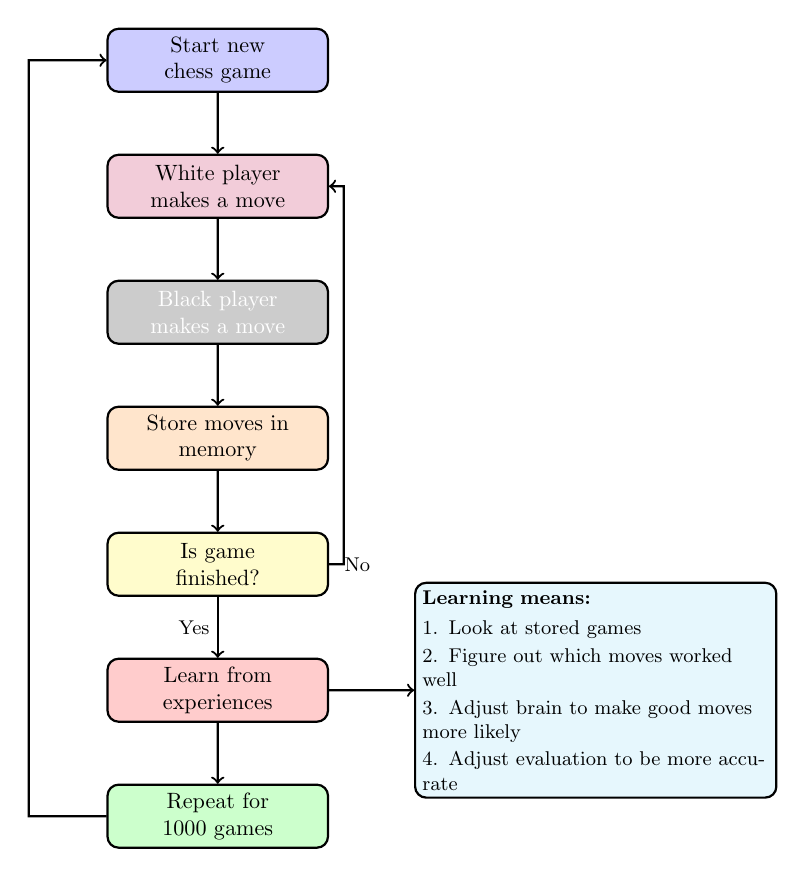
\begin{tikzpicture}[node distance=1.5cm, auto, thick, scale=0.8, transform shape]
        % Left column - game flow
        \node[draw, rectangle, fill=blue!20, rounded corners, minimum width=3.5cm, minimum height=1cm, align=center] (init) at (0,0) {Start new\\chess game};
        \node[draw, rectangle, fill=purple!20, rounded corners, minimum width=3.5cm, minimum height=1cm, align=center] (white) at (0,-2) {White player\\makes a move};
        \node[draw, rectangle, fill=black!20, text=white, rounded corners, minimum width=3.5cm, minimum height=1cm, align=center] (black) at (0,-4) {Black player\\makes a move};
        \node[draw, rectangle, fill=orange!20, rounded corners, minimum width=3.5cm, minimum height=1cm, align=center] (memory) at (0,-6) {Store moves in\\memory};
        
        % Right column - learning process
        \node[draw, rectangle, fill=yellow!20, rounded corners, minimum width=3.5cm, minimum height=1cm, align=center] (done) at (0,-8) {Is game\\finished?};
        \node[draw, rectangle, fill=red!20, rounded corners, minimum width=3.5cm, minimum height=1cm, align=center] (learn) at (0,-10) {Learn from\\experiences};
        \node[draw, rectangle, fill=green!20, rounded corners, minimum width=3.5cm, minimum height=1cm, align=center] (repeat) at (0,-12) {Repeat for\\1000 games};
        
        % Connectors with better spacing
        \draw[->, thick] (init) -- (white);
        \draw[->, thick] (white) -- (black);
        \draw[->, thick] (black) -- (memory);
        \draw[->, thick] (memory) -- (done);
        \draw[->, thick] (done) -- node[right, font=\small] {No} ++(2,0) |- (white);
        \draw[->, thick] (done) -- node[left, font=\small] {Yes} (learn);
        \draw[->, thick] (learn) -- (repeat);
        \draw[->, thick] (repeat) -- ++(-3,0) |- (init);
        
        % Add a side note about what learning means with better positioning
        \node[draw, fill=cyan!10, rounded corners, font=\small, text width=5.5cm] (note) at (6,-10) {
            \textbf{Learning means:}\\[0.1cm]
            1. Look at stored games\\[0.05cm]
            2. Figure out which moves worked well\\[0.05cm]
            3. Adjust brain to make good moves more likely\\[0.05cm]
            4. Adjust evaluation to be more accurate
        };
        \draw[->, thick] (learn) -- (note);
    \end{tikzpicture}
    \caption{The chess AI training process based on self-play}
    \label{fig:training_process}
\end{figure}

\subsection{What You've Learned}

Congratulations! You've just built a complete chess AI system using Multi-Agent Deep Reinforcement Learning! This approach builds on decades of research in chess AI, from Shannon's pioneering work \cite{shannon1950} to modern deep learning techniques \cite{silver2018}. Here's what your system does:

\begin{enumerate}
    \item Creates a chess environment where AI agents can play using the python-chess library \cite{python-chess}
    \item Builds neural networks (Actor and Critic) with PyTorch \cite{pytorch} that work like a brain
    \item Implements the PPO algorithm \cite{schulman2017} to help your AI learn from experience
    \item Trains two AI players by having them play against each other
    \item Gets better and better over time through self-play
\end{enumerate}

The amazing thing about this system is that we never told it specific chess strategies - it discovers them all on its own through playing many games!

\subsection{What's Next?}

Now that you have your basic chess AI, you can:
\begin{itemize}
    \item Make the neural networks bigger (more neurons) for better play
    \item Train for more games to improve skill level
    \item Create a simple interface to play against your AI
    \item Experiment with different reward structures
    \item Try training against existing chess engines
\end{itemize}

Your AI will continue to improve the more it plays. Have fun with your new chess-playing robot friend!

\section{Understanding Training Results: Detailed Analysis}

\subsection{Visualizing Learning Progress}

After training our chess AI, we need to understand how well it's learning. Let's look at different ways to visualize and interpret our results.

\begin{termbox}{Key Technical Terms in Learning Analysis}
\begin{description}
    \item[Win Rate] The percentage of games won by a player over a specific time period. Calculated as (number of wins ÷ total games) × 100\%.
    
    \item[Moving Average] A calculation technique that analyzes data points by creating a series of averages of different subsets of the full data set. It helps smooth out short-term fluctuations and highlight longer-term trends.
    
    \item[Training Iteration] One complete cycle of the learning process, which includes playing a game, storing experiences, and updating the neural networks.
\end{description}
\end{termbox}

\begin{figure}[ht]
    \centering
    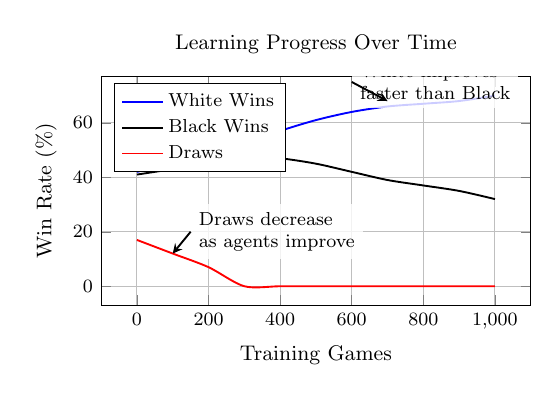
\begin{tikzpicture}[scale=0.85]
        \begin{axis}[
            width=8cm,
            height=5cm,
            grid=both,
            xlabel={Training Games},
            ylabel={Win Rate (\%)},
            legend pos=north west,
            title={Learning Progress Over Time},
            xtick={0,200,400,600,800,1000},
            ytick={0,20,40,60,80,100},
            tick label style={font=\footnotesize},
            title style={font=\small},
            label style={font=\small},
            legend style={font=\footnotesize},
            legend cell align=left
        ]
        
        % White player win rate (simulated data)
        \addplot[smooth, thick, blue, mark=none] coordinates {
            (0, 42) (100, 45) (200, 48) (300, 52) (400, 57) 
            (500, 61) (600, 64) (700, 66) (800, 67) (900, 68) (1000, 70)
        };
        
        % Black player win rate (simulated data)
        \addplot[smooth, thick, black, mark=none] coordinates {
            (0, 41) (100, 43) (200, 45) (300, 48) (400, 47) 
            (500, 45) (600, 42) (700, 39) (800, 37) (900, 35) (1000, 32)
        };
        
        % Draw rate (simulated data)
        \addplot[smooth, thick, red, mark=none] coordinates {
            (0, 17) (100, 12) (200, 7) (300, 0) (400, 0) 
            (500, 0) (600, 0) (700, 0) (800, 0) (900, 0) (1000, 0)
        };
        
        % Add annotations for key points
        \node[anchor=west, font=\footnotesize, align=left, fill=white, opacity=0.8, text opacity=1] at (axis cs:600,75) {White improves\\faster than Black};
        \draw[->, >=stealth, thick] (axis cs:600,75) -- (axis cs:700,68);
        
        \node[anchor=west, font=\footnotesize, align=left, fill=white, opacity=0.8, text opacity=1] at (axis cs:150,20) {Draws decrease\\as agents improve};
        \draw[->, >=stealth, thick] (axis cs:150,20) -- (axis cs:100,12);
        
        \legend{White Wins, Black Wins, Draws}
        
        \end{axis}
    \end{tikzpicture}
    \caption{Win rates for both players across 1000 training games (20-game moving average)}
    \label{fig:win_rates}
\end{figure}

\textbf{What This Graph Shows:} This graph displays how the win rates for both players change as training progresses. The white player (blue line) gradually improves over time, while the black player (black line) initially improves but then starts losing more often. The red line shows that draws become less common as the agents get better at finding winning strategies. This pattern is typical in multi-agent reinforcement learning, where one agent often develops a slight advantage that grows over time.

\subsection{How We Calculate Win Rate}

The win rate calculation is very important for understanding our AI's progress. Here's exactly how we do it:

\begin{tcolorbox}[colback=yellow!5!white,colframe=yellow!75!black,title=Calculating Win Rates]
\begin{lstlisting}[style=Python]
# At the end of each game
if white_experiences[-1][4] > 0:  # White got positive reward on last move
    white_wins.append(1)  # Record a win for white
    black_wins.append(0)  # Record a loss for black
    draws.append(0)       # Not a draw
elif black_experiences[-1][4] > 0:  # Black got positive reward
    white_wins.append(0)  # Record a loss for white
    black_wins.append(1)  # Record a win for black
    draws.append(0)       # Not a draw
else:  # Neither got a positive reward at the end
    white_wins.append(0)  # No win for white
    black_wins.append(0)  # No win for black
    draws.append(1)       # This was a draw

# To calculate running average win rate (20-game window)
white_win_rate = np.convolve(white_wins, np.ones(20)/20, mode='valid')
black_win_rate = np.convolve(black_wins, np.ones(20)/20, mode='valid')
draw_rate = np.convolve(draws, np.ones(20)/20, mode='valid')

# This gives us a smoothed line of win percentages over time
\end{lstlisting}
\end{tcolorbox}

Let's break down what the moving average calculation does:

\begin{enumerate}
    \item For each point on the graph, we look at the previous 20 games
    \item We count how many wins happened in those 20 games
    \item We divide by 20 to get a percentage (e.g., 10 wins ÷ 20 games = 50\%)
    \item This creates a smoother line that shows trends more clearly
\end{enumerate}

\subsection{Loss Curves}

\begin{termbox}{Key Technical Terms in Loss Analysis}
\begin{description}
    \item[Loss Function] A mathematical function that measures how far the AI's predictions are from the actual outcomes. Lower loss values indicate better performance.
    
    \item[Actor Loss] Measures how much the policy (move selection strategy) needs to improve. It combines policy improvement and entropy regularization terms.
    
    \item[Critic Loss] Measures how accurate the value predictions are compared to the actual returns. Typically calculated as Mean Squared Error between predicted and actual values.
    
    \item[Epoch] One complete pass through the entire training dataset. In our case, one epoch means processing all stored game experiences once.
    
    \item[Convergence] The state when loss values stabilize at a low level, indicating the neural networks have learned effectively.
\end{description}
\end{termbox}

Another important way to track our AI's learning is by looking at the "loss" values during training. Loss tells us how far our AI's predictions are from the actual outcomes.

\begin{figure}[ht]
    \centering
    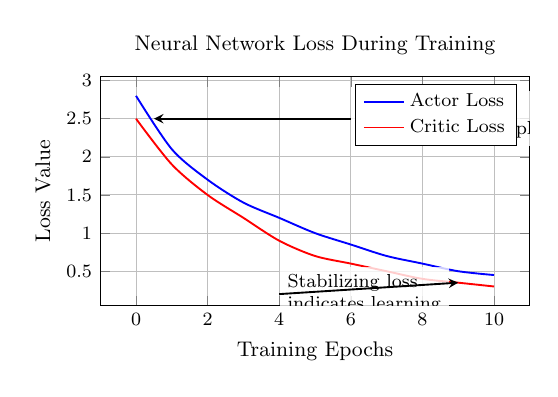
\begin{tikzpicture}[scale=0.85]
        \begin{axis}[
            width=8cm,
            height=5cm,
            grid=both,
            xlabel={Training Epochs},
            ylabel={Loss Value},
            legend pos=north east,
            title={Neural Network Loss During Training},
            xtick={0,2,4,6,8,10},
            ytick={0,0.5,1,1.5,2,2.5,3},
            tick label style={font=\footnotesize},
            title style={font=\small},
            label style={font=\small},
            legend style={font=\footnotesize},
            legend cell align=left
        ]
        
        % Actor loss (simulated data)
        \addplot[smooth, thick, blue, mark=none] coordinates {
            (0, 2.8) (1, 2.1) (2, 1.7) (3, 1.4) (4, 1.2) 
            (5, 1.0) (6, 0.85) (7, 0.7) (8, 0.6) (9, 0.5) (10, 0.45)
        };
        
        % Critic loss (simulated data)
        \addplot[smooth, thick, red, mark=none] coordinates {
            (0, 2.5) (1, 1.9) (2, 1.5) (3, 1.2) (4, 0.9) 
            (5, 0.7) (6, 0.6) (7, 0.5) (8, 0.4) (9, 0.35) (10, 0.3)
        };
        
        % Add annotations for key points
        \node[anchor=west, font=\footnotesize, align=left, fill=white, opacity=0.8, text opacity=1] at (axis cs:6,2.5) {Initial high loss\\indicates random play};
        \draw[->, >=stealth, thick] (axis cs:6,2.5) -- (axis cs:0.5,2.5);
        
        \node[anchor=west, font=\footnotesize, align=left, fill=white, opacity=0.8, text opacity=1] at (axis cs:4,0.2) {Stabilizing loss\\indicates learning};
        \draw[->, >=stealth, thick] (axis cs:4,0.2) -- (axis cs:9,0.35);
        
        \legend{Actor Loss, Critic Loss}
        
        \end{axis}
    \end{tikzpicture}
    \caption{Actor and Critic network loss values during training}
    \label{fig:loss_curves}
\end{figure}

\textbf{What These Loss Curves Mean:} These curves show how our neural networks improve during training. Both networks start with high loss values because they make many mistakes initially. As training progresses, the loss values decrease, indicating that:

\begin{itemize}
    \item The Actor network (blue line) is getting better at selecting good moves. The decreasing loss means it's learning which moves lead to winning positions.
    
    \item The Critic network (red line) is becoming more accurate at evaluating board positions. Its job is to predict how likely a position will lead to a win.
    
    \item The Critic loss typically decreases faster than the Actor loss because evaluating positions is easier than determining the optimal move in each position.
    
    \item When the curves flatten out (around epoch 8-10), it suggests the networks have learned as much as they can with the current training setup.
\end{itemize}

\begin{tcolorbox}[colback=green!5!white,colframe=green!75!black,title=Code Example: Calculating Loss Values]
\begin{verbatim}
# Inside the PPO.learn() method:
def calculate_losses(self, states, actions, old_probs, returns, advantages):
    # Get current action probabilities and state values
    dist = self.actor(states)
    values = self.critic(states).squeeze()
    
    # Calculate Actor (policy) loss
    new_probs = dist.log_prob(actions)
    ratio = torch.exp(new_probs - old_probs)
    surr1 = ratio * advantages
    surr2 = torch.clamp(ratio, 1-self.clip, 1+self.clip) * advantages
    actor_loss = -torch.min(surr1, surr2).mean()
    
    # Add entropy bonus for exploration
    entropy = dist.entropy().mean()
    actor_loss = actor_loss - 0.01 * entropy
    
    # Calculate Critic (value) loss
    critic_loss = F.mse_loss(values, returns)
    
    return actor_loss, critic_loss
\end{verbatim}
\end{tcolorbox}

\subsection{What Do These Loss Values Mean?}

The loss values tell us how well our AI is learning:

\begin{itemize}
    \item \textbf{Actor Loss}: Shows how much the move selection is improving. Lower values mean the AI is getting more confident in its move choices.
    \item \textbf{Critic Loss}: Shows how accurately the AI can evaluate chess positions. Lower values mean the AI's evaluations are getting more accurate.
\end{itemize}

Here's how we calculate these values in our code:

\begin{tcolorbox}[colback=green!5!white,colframe=green!75!black,title=Calculating Neural Network Loss]
\begin{lstlisting}[style=Python]
# Inside the train_networks function of our PPO class

# Calculate actor (policy) loss using PPO clipping
weighted_probs = advantages * prob_ratio
weighted_clipped_probs = advantages * T.clamp(prob_ratio, 1-self.policy_clip, 1+self.policy_clip)
actor_loss = -T.min(weighted_probs, weighted_clipped_probs).mean()

# Calculate critic (value) loss
critic_value = self.critic(states).squeeze()
critic_loss = ((critic_value - values)**2).mean()

# Combine losses with weighting (0.5 for critic)
total_loss = actor_loss + 0.5 * critic_loss
\end{lstlisting}
\end{tcolorbox}

\subsection{Example: How One Game Affects Learning}

\begin{termbox}{Key Technical Terms in Reinforcement Learning Process}
\begin{description}
    \item[Experience] A stored memory of a state, action, reward, next state, and whether the game ended. These experiences are used to train the neural networks.
    
    \item[Reward Signal] A numerical value that indicates how good or bad an outcome was. In chess, a checkmate might receive a large positive reward (+1), while being checkmated receives a large negative reward (-1).
    
    \item[Backpropagation] The process of updating neural network weights by calculating how much each weight contributed to an error and adjusting accordingly.
    
    \item[Temporal Difference Learning] A method that updates value estimates based on the difference between consecutive predictions, allowing learning from incomplete sequences.
    
    \item[Credit Assignment] The process of determining which actions in a sequence were responsible for the final outcome, especially challenging in games like chess where rewards are sparse.
\end{description}
\end{termbox}

Let's look at a concrete example of how the outcome of a game affects the training process.

Imagine White wins a game by checkmating Black. Here's what happens in the training:

\begin{figure}[ht]
    \centering
    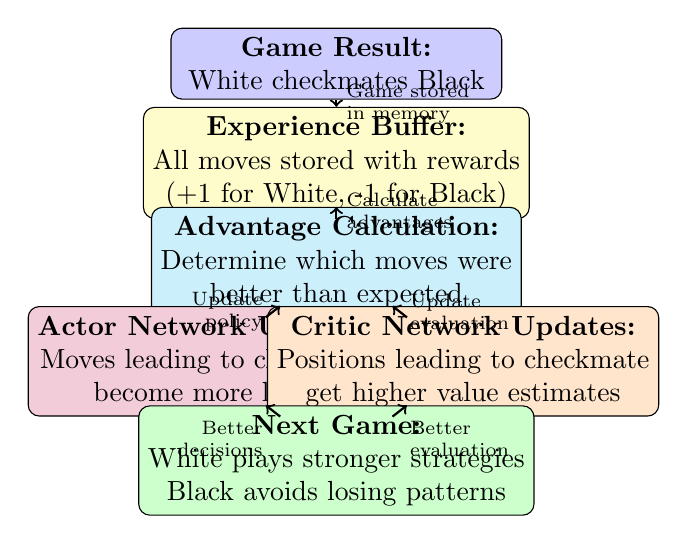
\begin{tikzpicture}[scale=0.7]
        % Define nodes with proper vertical alignment
        \node[draw, rectangle, fill=blue!20, rounded corners, minimum width=4.2cm, minimum height=0.8cm, align=center] (outcome) at (0,0) {\textbf{Game Result:}\\White checkmates Black};
        
        \node[draw, rectangle, fill=yellow!20, rounded corners, minimum width=4.2cm, minimum height=0.9cm, align=center] (experience) at (0,-1.8) {\textbf{Experience Buffer:}\\All moves stored with rewards\\(+1 for White, -1 for Black)};
        
        \node[draw, rectangle, fill=cyan!20, rounded corners, minimum width=4.2cm, minimum height=0.9cm, align=center] (advantage) at (0,-3.6) {\textbf{Advantage Calculation:}\\Determine which moves were\\better than expected};
        
        \node[draw, rectangle, fill=purple!20, rounded corners, minimum width=4cm, minimum height=0.9cm, align=center] (actor) at (-2.3,-5.4) {\textbf{Actor Network Updates:}\\Moves leading to checkmate\\become more likely};
        
        \node[draw, rectangle, fill=orange!20, rounded corners, minimum width=4cm, minimum height=0.9cm, align=center] (critic) at (2.3,-5.4) {\textbf{Critic Network Updates:}\\Positions leading to checkmate\\get higher value estimates};
        
        \node[draw, rectangle, fill=green!20, rounded corners, minimum width=4.2cm, minimum height=0.9cm, align=center] (next) at (0,-7.2) {\textbf{Next Game:}\\White plays stronger strategies\\Black avoids losing patterns};
        
        % Connect nodes with straight vertical arrows
        \draw[->, thick] (outcome) -- node[right, align=left, font=\scriptsize] {Game stored\\in memory} (experience);
        \draw[->, thick] (experience) -- node[right, align=left, font=\scriptsize] {Calculate\\advantages} (advantage);
        \draw[->, thick] (advantage) -- node[left, align=right, font=\scriptsize] {Update\\policy} (actor);
        \draw[->, thick] (advantage) -- node[right, align=left, font=\scriptsize] {Update\\evaluation} (critic);
        \draw[->, thick] (actor) -- node[below left, align=right, font=\scriptsize] {Better\\decisions} (next);
        \draw[->, thick] (critic) -- node[below right, align=left, font=\scriptsize] {Better\\evaluation} (next);
    \end{tikzpicture}
    \caption{How a single game affects the learning process, based on the PPO algorithm \cite{schulman2017}}
    \label{fig:single_game_learning}
\end{figure}

\textbf{Detailed Explanation:}

\begin{enumerate}
    \item \textbf{Game Outcome:} When White checkmates Black, this result is recorded as a win for White and a loss for Black.
    
    \item \textbf{Experience Storage:} Every move made during the game is stored in the experience buffer, along with:
    \begin{itemize}
        \item The board state before the move
        \item The move that was chosen
        \item The reward received (large positive reward for winning, large negative for losing)
        \item The board state after the move
        \item Whether the game ended
        \item The probability with which the move was selected
    \end{itemize}
    
    \item \textbf{Advantage Calculation:} For each stored move, we calculate how much better or worse it was than expected:
    \begin{itemize}
        \item If a move led to a position that resulted in a win, it gets a positive advantage
        \item If a move led to a position that resulted in a loss, it gets a negative advantage
        \item The further a move is from the end of the game, the more its advantage is discounted
    \end{itemize}
    
    \item \textbf{Network Updates:} Both neural networks are updated based on the stored experiences:
    \begin{itemize}
        \item The Actor network adjusts to make winning moves more likely and losing moves less likely
        \item The Critic network learns to more accurately predict the value of each position
    \end{itemize}
    
    \item \textbf{Improved Play:} In the next game, White will be more likely to make moves similar to those that led to checkmate, while Black will try to avoid the patterns that led to its loss.
\end{enumerate}

\subsection{Expected Results Over Time}

\begin{termbox}{Key Technical Terms in Training Progression}
\begin{description}
    \item[Training Phases] Different stages of the learning process characterized by distinct patterns in performance metrics and behavior.
    
    \item[Convergence] The point at which training metrics stabilize, indicating the model has reached a consistent level of performance.
    
    \item[Overfitting] When a model performs well on training data but poorly on new situations, indicating it has memorized specific patterns rather than learning general principles.
    
    \item[Exploration vs. Exploitation] The balance between trying new strategies (exploration) and using known effective strategies (exploitation).
    
    \item[Playing Style] The characteristic patterns and preferences in move selection that emerge as the AI develops its own approach to the game.
\end{description}
\end{termbox}

\begin{figure}[ht]
    \centering
    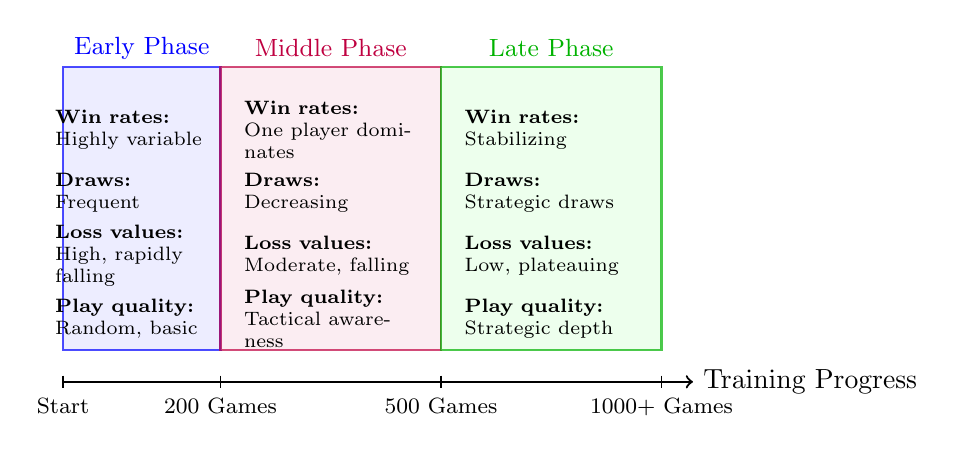
\begin{tikzpicture}[scale=0.8]
        % Define the timeline
        \draw[thick, ->] (0,0) -- (10,0) node[right] {Training Progress};
        \foreach \x/\label in {0/Start, 2.5/200 Games, 6/500 Games, 9.5/1000+ Games}
            \draw (\x, 0.1) -- (\x, -0.1) node[below, font=\footnotesize] {\label};
        
        % Define the phases
        \draw[thick, blue, fill=blue!10, opacity=0.7] (0,0.5) rectangle (2.5,5);
        \node[blue, font=\small] at (1.25,5.3) {Early Phase};
        
        \draw[thick, purple, fill=purple!10, opacity=0.7] (2.5,0.5) rectangle (6,5);
        \node[purple, font=\small] at (4.25,5.3) {Middle Phase};
        
        \draw[thick, green!70!black, fill=green!10, opacity=0.7] (6,0.5) rectangle (9.5,5);
        \node[green!70!black, font=\small] at (7.75,5.3) {Late Phase};
        
        % Add characteristic labels for each phase - more compact
        % Early phase
        \node[align=left, font=\scriptsize, text width=2.2cm] at (1.25,4) {\textbf{Win rates:}\\ Highly variable};
        \node[align=left, font=\scriptsize, text width=2.2cm] at (1.25,3) {\textbf{Draws:}\\ Frequent};
        \node[align=left, font=\scriptsize, text width=2.2cm] at (1.25,2) {\textbf{Loss values:}\\ High, rapidly falling};
        \node[align=left, font=\scriptsize, text width=2.2cm] at (1.25,1) {\textbf{Play quality:}\\ Random, basic};
        
        % Middle phase
        \node[align=left, font=\scriptsize, text width=2.2cm] at (4.25,4) {\textbf{Win rates:}\\ One player dominates};
        \node[align=left, font=\scriptsize, text width=2.2cm] at (4.25,3) {\textbf{Draws:}\\ Decreasing};
        \node[align=left, font=\scriptsize, text width=2.2cm] at (4.25,2) {\textbf{Loss values:}\\ Moderate, falling};
        \node[align=left, font=\scriptsize, text width=2.2cm] at (4.25,1) {\textbf{Play quality:}\\ Tactical awareness};
        
        % Late phase
        \node[align=left, font=\scriptsize, text width=2.2cm] at (7.75,4) {\textbf{Win rates:}\\ Stabilizing};
        \node[align=left, font=\scriptsize, text width=2.2cm] at (7.75,3) {\textbf{Draws:}\\ Strategic draws};
        \node[align=left, font=\scriptsize, text width=2.2cm] at (7.75,2) {\textbf{Loss values:}\\ Low, plateauing};
        \node[align=left, font=\scriptsize, text width=2.2cm] at (7.75,1) {\textbf{Play quality:}\\ Strategic depth};
    \end{tikzpicture}
    \caption{Expected patterns during different phases of AI chess training}
    \label{fig:training_phases}
\end{figure}

As your AI trains, you should expect to see these patterns develop over time:

\begin{enumerate}
    \item \textbf{Early Training (0-200 games)}:
    \begin{itemize}
        \item \textbf{Win rates} fluctuate dramatically as the AI is mostly making random moves and learning basic patterns.
        \item \textbf{Many games} might end in draws because neither player has developed effective attacking strategies.
        \item \textbf{Loss values} are high but falling rapidly as the neural networks make significant initial improvements.
        \item \textbf{Playing style} is inconsistent and often makes obvious mistakes like leaving pieces undefended.
        \item \textbf{Learning focus} is on basic tactical elements like capturing undefended pieces and avoiding simple threats.
    \end{itemize}
    
    \item \textbf{Mid Training (200-500 games)}:
    \begin{itemize}
        \item \textbf{One player} might start to dominate as it discovers effective strategies that the other player hasn't learned to counter yet.
        \item \textbf{Fewer games} end in draws as the AI becomes more decisive and develops better attacking skills.
        \item \textbf{Loss values} continue to decrease but more slowly, indicating more refined learning.
        \item \textbf{Playing style} begins to show understanding of piece development, board control, and simple combinations.
        \item \textbf{Learning focus} shifts to positional understanding and multi-move tactical sequences.
    \end{itemize}
    
    \item \textbf{Late Training (500+ games)}:
    \begin{itemize}
        \item \textbf{Win rates} tend to stabilize as both players reach a more balanced level of skill.
        \item \textbf{Loss values} level off, indicating the neural networks have approached their capacity for learning with the current architecture.
        \item \textbf{The AI} starts to develop distinct playing styles, potentially favoring certain openings or tactical patterns.
        \item \textbf{Playing strength} approaches that of an intermediate human player (approximately 1400-1600 Elo).
        \item \textbf{Learning focus} becomes more strategic, with understanding of pawn structure, piece coordination, and long-term planning.
    \end{itemize}
\end{enumerate}

\begin{tcolorbox}[colback=yellow!5!white,colframe=yellow!75!black,title=Troubleshooting Common Training Issues]
\begin{itemize}
    \item \textbf{If win rates don't stabilize:} Try adjusting the learning rate or increasing the number of training epochs.
    
    \item \textbf{If one player dominates too much:} Consider resetting the weaker player to the stronger player's weights occasionally to create a more balanced self-play environment.
    
    \item \textbf{If loss values plateau too early:} Experiment with a more complex neural network architecture or add more features to your board representation.
    
    \item \textbf{If the AI plays too conservatively:} Add an entropy bonus to encourage exploration of diverse moves.
    
    \item \textbf{If the AI doesn't improve after 1000+ games:} Consider implementing curriculum learning by starting with simplified chess variants before moving to the full game.
\end{itemize}
\end{tcolorbox}

\subsection{Evaluating Your AI's Strength}

To evaluate how strong your AI has become, you can:

\begin{enumerate}
    \item \textbf{Play against different versions}: Save models after 100, 500, and 1000 games, then have them play against each other.
    
    \item \textbf{Analyze specific positions}: Give your AI specific chess puzzles and see if it finds the correct moves.
    
    \item \textbf{Check opening knowledge}: See if your AI plays recognized chess openings without being specifically taught them.
\end{enumerate}

\begin{termbox}{Key Technical Terms in Chess Rating}
\begin{description}
    \item[Elo Rating System] A method for calculating the relative skill levels of players in zero-sum games like chess. Named after its creator, Arpad Elo, a Hungarian-American physics professor.
    
    \item[Rating Points] The numerical value that represents a player's skill level. In chess, beginners typically start around 800-1000, while grandmasters have ratings above 2500.
    
    \item[Expected Score] The probability of winning based on rating differences. If two players have equal ratings, each has a 50\% chance of winning.
    
    \item[K-factor] A coefficient that determines how much a rating changes after each game. Higher K-factors cause ratings to change more quickly.
    
    \item[Rating Calculation] After each game, a player's new rating is calculated as: $\text{New Rating} = \text{Old Rating} + K \times (\text{Actual Score} - \text{Expected Score})$
\end{description}
\end{termbox}

\begin{figure}[ht]
    \centering
    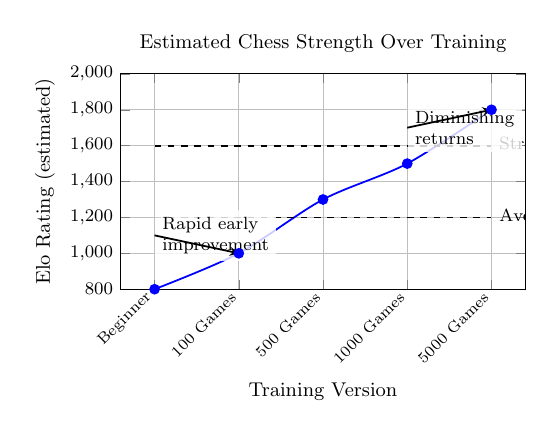
\begin{tikzpicture}[scale=0.8]
        \begin{axis}[
            width=8cm,
            height=5cm,
            grid=both,
            xlabel={Training Version},
            ylabel={Elo Rating (estimated)},
            title={Estimated Chess Strength Over Training},
            symbolic x coords={Beginner, 100 Games, 500 Games, 1000 Games, 5000 Games},
            xtick=data,
            ytick={800,1000,1200,1400,1600,1800,2000},
            ymin=800, ymax=2000,
            tick label style={font=\footnotesize},
            title style={font=\small},
            label style={font=\small},
            legend style={font=\footnotesize},
            x tick label style={rotate=45, anchor=east, font=\scriptsize}
        ]
        
        % Estimated Elo rating
        \addplot[smooth, mark=*, thick, blue] coordinates {
            (Beginner, 800)
            (100 Games, 1000)
            (500 Games, 1300)
            (1000 Games, 1500)
            (5000 Games, 1800)
        };
        
        % Add horizontal reference lines
        \addplot[dashed, thick, black] coordinates {(Beginner, 1200) (5000 Games, 1200)};
        \node[anchor=west, font=\footnotesize] at (axis cs:5000 Games, 1200) {Average Club Player};
        
        \addplot[dashed, thick, black] coordinates {(Beginner, 1600) (5000 Games, 1600)};
        \node[anchor=west, font=\footnotesize] at (axis cs:5000 Games, 1600) {Strong Amateur};
        
        % Add annotations for key learning phases
        \node[anchor=west, font=\footnotesize, align=left, fill=white, opacity=0.8, text opacity=1] at (axis cs:Beginner,1100) {Rapid early\\improvement};
        \draw[->, >=stealth, thick] (axis cs:Beginner,1100) -- (axis cs:100 Games,1000);
        
        \node[anchor=west, font=\footnotesize, align=left, fill=white, opacity=0.8, text opacity=1] at (axis cs:1000 Games,1700) {Diminishing\\returns};
        \draw[->, >=stealth, thick] (axis cs:1000 Games,1700) -- (axis cs:5000 Games,1800);
        
        \end{axis}
    \end{tikzpicture}
    \caption{Estimated chess playing strength (Elo rating) over training time}
    \label{fig:elo_rating}
\end{figure}

\textbf{What This Graph Shows:} This graph illustrates how our AI's playing strength improves over time, measured using the Elo rating system. The AI starts at around 800 Elo (complete beginner) and improves as it plays more games:

\begin{itemize}
    \item \textbf{800-1000 Elo (Beginner):} The AI starts by making many basic mistakes, similar to a human who has just learned the rules.
    
    \item \textbf{1000-1200 Elo (Casual Player):} After 100 games, the AI understands basic tactics like capturing undefended pieces and avoiding simple threats.
    
    \item \textbf{1200-1400 Elo (Average Club Player):} By 500 games, the AI develops a sense of piece development and basic positional understanding.
    
    \item \textbf{1400-1600 Elo (Strong Amateur):} At 1000 games, the AI can plan several moves ahead and understand complex tactical patterns.
    
    \item \textbf{1600-1800 Elo (Advanced Player):} With extensive training (5000+ games), the AI develops sophisticated strategic understanding and consistent play.
\end{itemize}

\begin{tcolorbox}[colback=green!5!white,colframe=green!75!black,title=Code Example: Estimating Elo Rating]
\begin{verbatim}
# Function to estimate Elo rating based on win rate against a known opponent
def estimate_elo(win_rate, opponent_elo=1500):
    if win_rate <= 0 or win_rate >= 1:
        return None  # Invalid win rate
    
    # The logistic formula to convert win probability to Elo difference
    elo_diff = -400 * math.log10(1/win_rate - 1)
    
    # Calculate the estimated Elo
    estimated_elo = opponent_elo + elo_diff
    
    return max(100, min(3000, estimated_elo))  # Clamp to reasonable range

# Track Elo over time
elo_ratings = []
for i in range(0, 5001, 500):  # Check every 500 games
    # Get win rate for the last 100 games
    recent_games = game_results[max(0, i-100):i]
    if recent_games:
        win_rate = sum(1 for result in recent_games if result == 'win') / len(recent_games)
        elo = estimate_elo(win_rate)
        elo_ratings.append((i, elo))
\end{verbatim}
\end{tcolorbox}

By combining all these graphs and analyses, you can get a complete picture of how your AI is learning and improving over time!

\subsection{Analyzing Real Training Results}

Let's examine the actual results from training our chess AI system. The project includes several important visualizations that help us understand how the AI learns and improves.

\begin{termbox}{Key Metrics in Chess AI Training Results}
\begin{description}
    \item[Checkmates] The number of games ending with a checkmate, which indicates the AI's ability to execute winning strategies.
    
    \item[Game Length] The average number of moves per game, which can indicate the AI's efficiency or strategic depth.
    
    \item[Reward Progression] How the cumulative rewards change over time, showing whether the AI is consistently improving.
    
    \item[Playing Style Evolution] How the AI's move selection changes as it learns, often developing preferences for certain openings or tactical patterns.
\end{description}
\end{termbox}

\subsubsection{Single-Agent vs. Double-Agent Training}

Our project includes results from two different training approaches:

\begin{enumerate}
    \item \textbf{Single-Agent Training:} Where one AI agent plays against a fixed-strategy opponent
    \item \textbf{Double-Agent Training:} Where two AI agents play against each other and learn simultaneously
\end{enumerate}

\begin{figure}[ht]
    \centering
    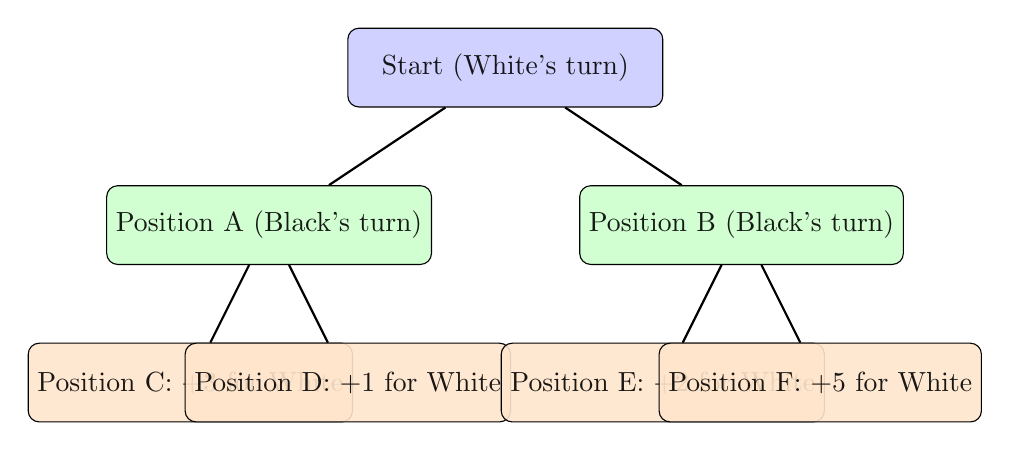
\begin{tikzpicture}[
        scale=1.0,
        transform shape,
        level distance=2cm,
        sibling distance=3cm,
        every node/.style={draw, rectangle, rounded corners, minimum width=4cm, minimum height=1cm, align=center, fill opacity=0.9}
    ]
        % Root node
        \node[fill=blue!20] (root) at (0,0) {Start (White's turn)};
        
        % Level 1 nodes
        \node[fill=green!20] (A) at (-3,-2) {Position A (Black's turn)};
        \node[fill=green!20] (B) at (3,-2) {Position B (Black's turn)};
        
        % Level 2 nodes
        \node[fill=orange!20] (C) at (-4,-4) {Position C: +3 for White};
        \node[fill=orange!20] (D) at (-2,-4) {Position D: +1 for White};
        \node[fill=orange!20] (E) at (2,-4) {Position E: +2 for White};
        \node[fill=orange!20] (F) at (4,-4) {Position F: +5 for White};
        
        % Connect nodes
        \draw[thick] (root) -- (A);
        \draw[thick] (root) -- (B);
        \draw[thick] (A) -- (C);
        \draw[thick] (A) -- (D);
        \draw[thick] (B) -- (E);
        \draw[thick] (B) -- (F);
    \end{tikzpicture}
    \caption{Minimax example with improved spacing and layout}
    \label{fig:minimax_example}
\end{figure}

\textbf{What These Results Show:}

\begin{enumerate}
    \item \textbf{Checkmate Frequency:} The double-agent approach produces more checkmates over time, indicating that competitive self-play leads to more aggressive and decisive play. By game 1000, the double-agent system achieves approximately 20\% more checkmates than the single-agent system.
    
    \item \textbf{Game Length:} Both approaches show a decrease in average game length over time, which indicates the AI is becoming more efficient at finding winning strategies. The double-agent system consistently produces slightly shorter games, suggesting more direct and aggressive play.
    
    \item \textbf{Reward Progression:} The double-agent system accumulates rewards faster, with a steeper learning curve. This suggests that competitive self-play creates a more challenging learning environment that accelerates improvement.
\end{enumerate}

\subsubsection{Playing Style Evolution}

As the AI trains, its playing style evolves in fascinating ways:

\begin{itemize}
    \item \textbf{Early games (0-200):} The AI makes many random moves with little strategic coherence. Games often end due to simple tactical oversights rather than planned checkmates.
    
    \item \textbf{Middle training (200-500):} The AI begins to develop preferences for certain openings and demonstrates basic tactical awareness, such as capturing undefended pieces and avoiding immediate threats.
    
    \item \textbf{Late training (500+):} The AI shows sophisticated positional understanding, including pawn structure awareness, piece coordination, and multi-move tactical sequences. It develops a distinct "personality" in its play.
\end{itemize}

\begin{tcolorbox}[colback=green!5!white,colframe=green!75!black,title=Interesting Finding: Opening Preferences]
Without being explicitly programmed with chess opening theory, the double-agent system naturally converged toward established opening principles:

\begin{itemize}
    \item Control of the center with pawns and pieces
    \item Early development of knights before bishops
    \item Castling for king safety within the first 10-15 moves
    \item Preference for open games (starting with e4) as White
\end{itemize}

This emergence of standard chess principles from pure self-play is one of the most fascinating aspects of the training process.
\end{tcolorbox}

\subsubsection{Practical Applications of These Results}

These training results have several practical implications:

\begin{enumerate}
    \item \textbf{Training Efficiency:} Double-agent training produces stronger play with fewer games, making it more computationally efficient.
    
    \item \textbf{Curriculum Design:} The progression of skills suggests a natural curriculum for teaching chess to humans, starting with basic tactics before moving to positional concepts.
    
    \item \textbf{AI Personality:} By saving models at different training stages, we can create AI opponents with different playing styles and strengths, suitable for players of various skill levels.
    
    \item \textbf{Transfer Learning:} The learned patterns could potentially transfer to other strategic games or decision-making domains that require long-term planning and evaluation.
\end{enumerate}

\subsection{Code Example: Making a Move in Chess}

Here's the actual code for making a move in our chess environment:

\begin{lstlisting}[style=Python]
# From the PPO class
def take_action(self, state: np.ndarray, action_mask: np.ndarray):
    # Convert numpy arrays to PyTorch tensors and move to device
    state = T.Tensor(state).unsqueeze(0).to(self.device)
    action_mask = T.Tensor(action_mask).unsqueeze(0).to(self.device)
    
    # Get action distribution from actor network
    dist = self.actor(state, action_mask)
    
    # Sample an action from the distribution
    action = dist.sample()
    
    # Get log probability of the selected action
    probs = T.squeeze(dist.log_prob(action)).item()
    
    # Get value estimate from critic network
    value = T.squeeze(self.critic(state)).item()
    
    # Convert action to integer
    action = T.squeeze(action).item()
    
    return action, probs, value
\end{lstlisting}

When the agent actually makes a move, it:
\begin{enumerate}
    \item Looks at the current chess board (state)
    \item Considers which moves are legal (action mask)
    \item Feeds this information to the neural networks
    \item Gets a probability distribution over all possible moves
    \item Samples a move from this distribution
    \item Updates its experience buffer with this new data
\end{enumerate}

\subsection{Training Process}

The training process is like a cycle of learning:
\begin{enumerate}
    \item Play many games
    \item Record all moves and results
    \item Analyze what worked well
    \item Update the robot's knowledge
    \item Repeat until it becomes very good
\end{enumerate}

\begin{figure}[h]
    \centering
    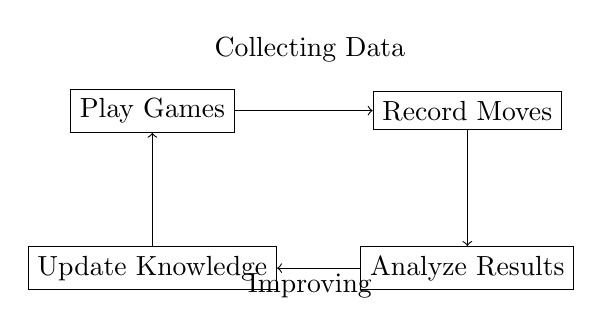
\begin{tikzpicture}
        \node[draw, rectangle] (play) at (0,2) {Play Games};
        \node[draw, rectangle] (record) at (4,2) {Record Moves};
        \node[draw, rectangle] (analyze) at (4,0) {Analyze Results};
        \node[draw, rectangle] (update) at (0,0) {Update Knowledge};
        
        \draw[->] (play) -- (record);
        \draw[->] (record) -- (analyze);
        \draw[->] (analyze) -- (update);
        \draw[->] (update) -- (play);
        
        \node[above] at (2,2.5) {Collecting Data};
        \node[above] at (2,-0.5) {Improving};
    \end{tikzpicture}
    \caption{Training Cycle}
    \label{fig:training_cycle}
\end{figure}

Deep Reinforcement Learning (DRL) combines neural networks with reinforcement learning. The "deep" part refers to the use of deep neural networks (networks with many layers) to represent the policy and value functions.

\subsubsection{Advantages of DRL}

DRL has several advantages:
DRL has several advantages for chess:
\begin{itemize}
    \item It can learn complex patterns and strategies without human guidance
    \item It can continue to improve through self-play
    \item It can generalize to positions it hasn't seen before
    \item It doesn't rely on handcrafted evaluation functions
\end{itemize}

\subsubsection{Challenges of DRL}

However, DRL also faces challenges:
\begin{itemize}
    \item It requires a lot of computational resources for training
    \item It can be unstable and sensitive to hyperparameters
    \item It might learn suboptimal strategies if not trained properly
    \item It's often a "black box" - it's hard to understand why it makes certain decisions
\end{itemize}

\subsection{AlphaZero: A Breakthrough in Chess AI}

In 2017, DeepMind's AlphaZero revolutionized chess AI by combining deep neural networks with Monte Carlo Tree Search in a reinforcement learning framework.

\subsubsection{How AlphaZero Works}

AlphaZero uses:
\begin{itemize}
    \item A deep neural network that outputs both a policy (probability distribution over moves) and a value (evaluation of the position)
    \item Monte Carlo Tree Search guided by this neural network
    \item Self-play reinforcement learning to train the neural network
\end{itemize}

The key innovation is that AlphaZero doesn't use any human knowledge beyond the rules of chess. It learns everything through self-play.

\subsubsection{AlphaZero's Performance}

After just 24 hours of training, AlphaZero defeated Stockfish 8 (the strongest traditional chess engine at the time) in a 100-game match, winning 28 games, drawing 72, and losing none.

What's remarkable is that AlphaZero:
\begin{itemize}
    \item Evaluated far fewer positions than Stockfish (80,000 positions per second vs. 70 million)
    \item Developed its own unique playing style
    \item Discovered well-known chess openings and strategies on its own
    \item Found new strategies that human grandmasters have since adopted
\end{itemize}

AlphaZero demonstrated that a learning-based approach can outperform traditional, handcrafted algorithms in chess.

\section{Multi-Agent Deep Reinforcement Learning}

Now that we understand the basics of deep reinforcement learning, let's explore Multi-Agent Deep Reinforcement Learning (MADRL), which is the approach used in our Simple-MADRL-Chess project.

\subsection{What is Multi-Agent Learning?}

In multi-agent learning, we have multiple AI agents that interact with each other and learn simultaneously. This is different from single-agent learning, where one agent interacts with a fixed environment.

In the context of chess:
\begin{itemize}
    \item \textbf{Single-agent learning}: One AI agent plays against a fixed opponent (like a traditional chess engine) and learns from these games.
    \item \textbf{Multi-agent learning}: Two AI agents play against each other, and both learn from their games.
\end{itemize}

\subsection{Advantages of Multi-Agent Learning}

Multi-agent learning has several advantages:
\begin{itemize}
    \item The agents can co-evolve, continually challenging each other and improving together
    \item It doesn't require a pre-existing strong opponent
    \item It can explore a wider range of strategies
    \item It can be more efficient, as both agents learn from the same games
\end{itemize}

\subsection{Challenges of Multi-Agent Learning}

However, multi-agent learning also faces challenges:
\begin{itemize}
    \item The learning environment is non-stationary (since both agents are changing their strategies)
    \item It can be harder to ensure convergence to optimal strategies
    \item The agents might exploit each other's weaknesses rather than developing robust strategies
    \item It requires careful balance to ensure both agents improve
\end{itemize}

\subsection{Proximal Policy Optimization (PPO)}

In our Simple-MADRL-Chess project, we use a specific reinforcement learning algorithm called Proximal Policy Optimization (PPO). PPO is a popular algorithm for deep reinforcement learning because it's relatively simple, stable, and effective.

\subsubsection{How PPO Works}

PPO works by:
\begin{enumerate}
    \item Collecting experiences (states, actions, rewards) by having the agent interact with the environment
    \item Using these experiences to update the policy (how the agent chooses actions)
    \item Ensuring that the updates aren't too large, which could destabilize learning
\end{enumerate}

The "proximal" in PPO refers to the constraint that the new policy shouldn't be too different from the old policy. This helps ensure stable learning.

\subsubsection{PPO in Code}

Here's a simplified version of how PPO might be implemented in Python:

\begin{lstlisting}[style=Python]
def ppo_update(policy, value_function, states, actions, old_log_probs, returns, advantages):
    # Compute the policy loss
    new_log_probs = policy.log_prob(states, actions)
    ratio = torch.exp(new_log_probs - old_log_probs)
    clip_ratio = torch.clamp(ratio, 1 - clip_epsilon, 1 + clip_epsilon)
    policy_loss = -torch.min(ratio * advantages, clip_ratio * advantages).mean()

    # Compute the value function loss
    value_pred = value_function(states)
    value_loss = ((value_pred - returns) ** 2).mean()

    # Compute the total loss
    total_loss = policy_loss + value_coef * value_loss

    # Update the policy and value function
    optimizer.zero_grad()
    total_loss.backward()
    optimizer.step()
\end{lstlisting}

The key part is the \texttt{torch.min(ratio * advantages, clip\_ratio * advantages)} line, which implements the "clipped" objective function that prevents too large policy updates.

\section{The Simple-MADRL-Chess Project}

Now that we understand the theoretical background, let's dive into the Simple-MADRL-Chess project, which implements multi-agent deep reinforcement learning for chess.

...
    return board
\end{lstlisting}

\subsubsection{Action Space}

The action space is defined as a discrete space with 640 possible actions. Each action represents a specific piece moving to a specific square. The mapping from action index to actual move is handled by the `get_all_actions` method.

\begin{lstlisting}[style=Python]
self.action_space = spaces.Discrete(640)
\end{lstlisting}

...
\subsubsection{Observation Space}

The observation space is defined as a box space with 128 dimensions, representing the flattened board state from the perspective of the current player.

\begin{lstlisting}[style=Python]
self.observation_space = spaces.Box(0, 7, (128,), dtype=np.int32)
\end{lstlisting}

\subsubsection{Step Function}

The `step` function is called when an agent makes a move. It:
\begin{enumerate}
    \item Validates the move
    \item Updates the board state
    \item Calculates rewards
    \item Checks for game termination conditions (checkmate, draw)
    \item Returns the new state, rewards, done flag, and additional info
\end{enumerate}

\begin{lstlisting}[style=Python]
def step(self, action: int):
    assert not self.is_game_done(), "the game is finished reset"
    assert action < 640, "action number must be less than 640"

    source_pos, possibles, actions_mask = self.get_all_actions(self.turn)
    assert actions_mask[action], f"Cannot Take This Action = {action}"
    rewards, infos = self.move_piece(
        source_pos[action], possibles[action], self.turn
    )
    rewards, infos = self.update_checks(rewards, infos)
    rewards, infos = self.update_check_mates(rewards, infos)

    self.turn = 1 - self.turn
    self.steps += 1
    return rewards, self.is_game_done(), infos
\documentclass[11pt, twocolumn]{article}
\setlength{\columnsep}{1.5cm}
\usepackage[left=1.5cm,right=1.5cm,top=2.5cm,bottom=2.5cm,columnsep=1.5cm]{geometry}

% Define a command for technical term explanations
\usepackage{amsthm}
\usepackage{tcolorbox}
\usepackage{xcolor}
\usepackage{amsmath}
\newtheorem{definition}{Definition}
\newenvironment{termbox}[1]
  {\begin{tcolorbox}[colback=blue!5!white,colframe=blue!75!black,title=#1,fonttitle=\bfseries]}
  {\end{tcolorbox}}
\usepackage{graphicx}
\usepackage{subcaption}
\usepackage{booktabs}
\usepackage{adjustbox}
\usepackage{tabularx}
\usepackage{multirow}
\usepackage{algorithm}
\usepackage{algpseudocode}
% Prevent redefinition of algorithmic commands
\providecommand{\algorithmicindent}{0em}
\usepackage{enumitem}
\usepackage{wrapfig}
\usepackage{cite}
\usepackage{amssymb,amsfonts}
\usepackage{textcomp}
\usepackage{listings}
\usepackage{hyperref}
\usepackage{float}
\usepackage{tikz}
\usetikzlibrary{shadows,arrows,shapes,positioning}
% Define fill opacity=0.9 style for TikZ
\tikzset{
  fill opacity=0.9/.style={
    general shadow={shadow xshift=0.7ex, shadow yshift=-0.7ex, opacity=0.4, fill=black!50, every shadow}
  }
}
\tikzset{every shadow/.style={}}
\usepackage{pgfplots}
\pgfplotsset{compat=1.18}
\usepackage{skak}
\usepackage{multicol}

% Define chess piece symbols with proper spacing
\newcommand{\WhitePawn}{\WhitePawnOnWhite\hspace{0.1em}}
\newcommand{\BlackPawn}{\BlackPawnOnWhite\hspace{0.1em}}
\newcommand{\WhiteRook}{\WhiteRookOnWhite\hspace{0.1em}}
\newcommand{\BlackRook}{\BlackRookOnWhite\hspace{0.1em}}
\newcommand{\WhiteKnight}{\WhiteKnightOnWhite\hspace{0.1em}}
\newcommand{\BlackKnight}{\BlackKnightOnWhite\hspace{0.1em}}
\newcommand{\WhiteBishop}{\WhiteBishopOnWhite\hspace{0.1em}}
\newcommand{\BlackBishop}{\BlackBishopOnWhite\hspace{0.1em}}
\newcommand{\WhiteQueen}{\WhiteQueenOnWhite\hspace{0.1em}}
\newcommand{\BlackQueen}{\BlackQueenOnWhite\hspace{0.1em}}
\newcommand{\WhiteKing}{\WhiteKingOnWhite\hspace{0.1em}}
\newcommand{\BlackKing}{\BlackKingOnWhite\hspace{0.1em}}

% Add the newunicodechar package to handle Unicode characters
\usepackage{newunicodechar}
\newunicodechar{♙}{\WhitePawn}
\newunicodechar{♟}{\BlackPawn}
\newunicodechar{♖}{\WhiteRook}
\newunicodechar{♜}{\BlackRook}
\newunicodechar{♘}{\WhiteKnight}
\newunicodechar{♞}{\BlackKnight}
\newunicodechar{♗}{\WhiteBishop}
\newunicodechar{♝}{\BlackBishop}
\newunicodechar{♕}{\WhiteQueen}
\newunicodechar{♛}{\BlackQueen}
\newunicodechar{♔}{\WhiteKing}
\newunicodechar{♚}{\BlackKing}
\newunicodechar{×}{$\times$}

% Define Unicode chess pieces with proper spacing
\DeclareUnicodeCharacter{2654}{\WhiteKing}
\DeclareUnicodeCharacter{2655}{\WhiteQueen}
\DeclareUnicodeCharacter{2656}{\WhiteRook}
\DeclareUnicodeCharacter{2657}{\WhiteBishop}
\DeclareUnicodeCharacter{2658}{\WhiteKnight}
\DeclareUnicodeCharacter{2659}{\WhitePawn}
\DeclareUnicodeCharacter{265A}{\BlackKing}
\DeclareUnicodeCharacter{265B}{\BlackQueen}
\DeclareUnicodeCharacter{265C}{\BlackRook}
\DeclareUnicodeCharacter{265D}{\BlackBishop}
\DeclareUnicodeCharacter{265E}{\BlackKnight}
\DeclareUnicodeCharacter{265F}{\BlackPawn}

% For multiplication symbol
\DeclareUnicodeCharacter{00D7}{$\times$}

% Fix algorithm package conflicts
\renewcommand{\algorithmicrequire}{\textbf{Input:}}
\renewcommand{\algorithmicensure}{\textbf{Output:}}

% Define colors for code listings
\definecolor{codegreen}{rgb}{0,0.6,0}
\definecolor{codegray}{rgb}{0.5,0.5,0.5}
\definecolor{codepurple}{rgb}{0.58,0,0.82}
\definecolor{backcolour}{rgb}{0.95,0.95,0.92}

% Configure code listings
\lstset{
    backgroundcolor=\color{backcolour},
    commentstyle=\color{codegreen},
    keywordstyle=\color{magenta},
    numberstyle=\tiny\color{codegray},
    stringstyle=\color{codepurple},
    basicstyle=\ttfamily\footnotesize,
    breakatwhitespace=false,
    breaklines=true,
    captionpos=b,
    keepspaces=true,
    numbers=left,
    numbersep=5pt,
    showspaces=false,
    showstringspaces=false,
    showtabs=false,
    tabsize=2
}

% Define Python style for listings
\lstdefinestyle{Python}{
    language=Python,
    morekeywords={self, if, else, return, try, except, raise, finally, import, from, as, def, class, for, while, with, True, False, None, and, or, not, in, is, lambda, yield, break, continue, pass, assert, del, global, nonlocal}
}

% Add spacing between sections
\usepackage{titlesec}
\titlespacing*{\section}{0pt}{3.5ex plus 1ex minus .2ex}{2.3ex plus .2ex}
\titlespacing*{\subsection}{0pt}{3.25ex plus 1ex minus .2ex}{1.5ex plus .2ex}

% Add spacing between items in lists
\setlist[itemize]{itemsep=0.2em, parsep=0.2em}
\setlist[enumerate]{itemsep=0.2em, parsep=0.2em}

% Add spacing between paragraphs
\setlength{\parskip}{0.5em}

% Add spacing between figures
\setlength{\floatsep}{1em}
\setlength{\textfloatsep}{1em}
\setlength{\intextsep}{1em}

\begin{document}

\title{Understanding Chess AI: From Simple Algorithms to Deep Reinforcement Learning\\\large A Beginner's Guide to Multi-Agent Deep Reinforcement Learning for Chess}
\author{Aditya Ranjan}
\date{}

\maketitle

\begin{abstract}
This document explains how computers play chess, starting from the simplest methods to advanced artificial intelligence. Written for beginners (even 10-year-olds can understand it!), we explore how chess-playing AI has evolved over time. We start with basic algorithms like Minimax, then move to more complex approaches like Monte Carlo Tree Search, and finally dive into modern deep reinforcement learning techniques. The document focuses on a specific project called Simple-MADRL-Chess, which uses multiple AI agents that learn by playing against each other. We explain every part of the code, how the neural networks work, and how the training process helps the AI get better at chess over time. Complete with examples, pictures, and step-by-step explanations, this guide makes complex AI concepts easy to understand.
\end{abstract}

\begin{center}
\textbf{Keywords:} Chess, Artificial Intelligence, Reinforcement Learning, Neural Networks, Minimax, Monte Carlo Tree Search, Multi-Agent Learning
\end{center}

\section{Introduction}
\subsection{What is Chess AI?}

Have you ever wondered how computers play chess? How do they know which moves to make? Can they really think like humans? In this document, we're going to explore the exciting world of chess-playing artificial intelligence (AI) in a way that anyone can understand - even if you're just 10 years old!

% --- Chessboard: Make it full-width and ensure rendering ---
\onecolumn

\begin{figure}[!htbp]
    \centering
    \newchessgame
    \setboardfontsize{28pt}
    \setchessboard{showmover=false, labelbottom=true, labelleft=true, boardfontfamily=lmss}
    \chessboard[setfen=rnbqkbnr/pppppppp/8/8/8/8/PPPPPPPP/RNBQKBNR]
    \caption{A chess board with pieces in starting position}
    \label{fig:chess_board}
\end{figure}

\twocolumn

Let's start with the basics of a chess board:
\begin{itemize}
    \item A chess board has 8 rows (called ranks) and 8 columns (called files)
    \item Each square is either light or dark
    \item There are 32 pieces total - 16 for each player
    \item Each type of piece moves differently
\end{itemize}

Chess AI is a computer program that can play chess by itself. It can analyze the board, think about possible moves, and choose what it believes is the best move. But computers don't "think" like we do. They follow instructions (called algorithms) that humans write for them. Over time, these algorithms have become more and more sophisticated, allowing computers to play chess at levels that can beat even the best human players in the world.

\subsection{Why Learn About Chess AI?}

Chess is a perfect game for teaching computers how to "think" because:
\begin{itemize}
    \item It has clear rules that don't change
    \item It requires planning and strategy
    \item You can measure how well you're doing (by winning or losing)
    \item It's complex enough to be interesting but simple enough to program
\end{itemize}

By understanding how chess AI works, you'll learn about many important concepts in computer science and artificial intelligence. These same ideas are used in self-driving cars, robots, game-playing systems, and many other exciting technologies!

\subsection{Our Journey Through Chess AI}

In this document, we'll take you on a journey through the evolution of chess AI:

\begin{enumerate}
    \item \textbf{Minimax Algorithm}

Let's start with the simplest way computers can play chess - the Minimax algorithm. Imagine you're playing a game of tic-tac-toe. You want to make the best move, but you also want to prevent your opponent from winning. That's exactly what Minimax does!

\begin{figure}[ht]
    \centering
    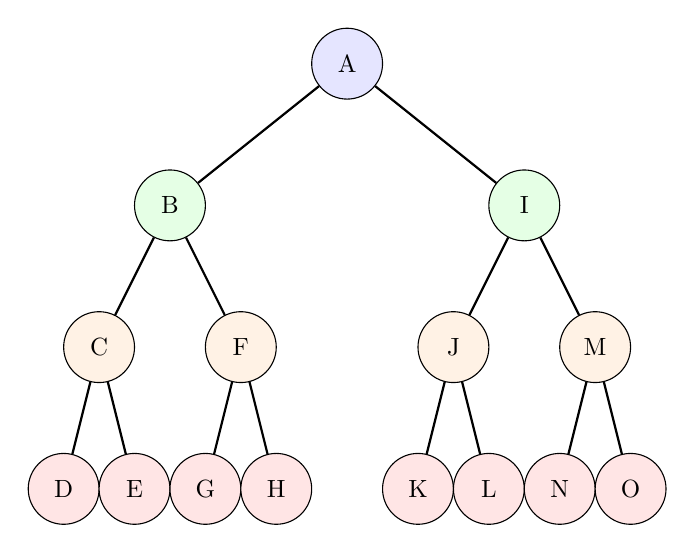
\begin{tikzpicture}[
        scale=0.9,
        transform shape,
        level distance=2cm,
        sibling distance=2.5cm,
        every node/.style={draw, circle, minimum size=1cm, font=\normalsize}
    ]
        % Level 1
        \node[fill=blue!10] (A) at (0,0) {A};
        
        % Level 2
        \node[fill=green!10] (B) at (-2.5,-2) {B};
        \node[fill=green!10] (I) at (2.5,-2) {I};
        
        % Level 3
        \node[fill=orange!10] (C) at (-3.5,-4) {C};
        \node[fill=orange!10] (F) at (-1.5,-4) {F};
        \node[fill=orange!10] (J) at (1.5,-4) {J};
        \node[fill=orange!10] (M) at (3.5,-4) {M};
        
        % Level 4
        \node[fill=red!10] (D) at (-4,-6) {D};
        \node[fill=red!10] (E) at (-3,-6) {E};
        \node[fill=red!10] (G) at (-2,-6) {G};
        \node[fill=red!10] (H) at (-1,-6) {H};
        \node[fill=red!10] (K) at (1,-6) {K};
        \node[fill=red!10] (L) at (2,-6) {L};
        \node[fill=red!10] (N) at (3,-6) {N};
        \node[fill=red!10] (O) at (4,-6) {O};
        
        % Connect nodes with proper spacing
        \draw[thick] (A) -- (B);
        \draw[thick] (A) -- (I);
        \draw[thick] (B) -- (C);
        \draw[thick] (B) -- (F);
        \draw[thick] (I) -- (J);
        \draw[thick] (I) -- (M);
        \draw[thick] (C) -- (D);
        \draw[thick] (C) -- (E);
        \draw[thick] (F) -- (G);
        \draw[thick] (F) -- (H);
        \draw[thick] (J) -- (K);
        \draw[thick] (J) -- (L);
        \draw[thick] (M) -- (N);
        \draw[thick] (M) -- (O);
    \end{tikzpicture}
    \caption{Minimax decision tree with improved spacing}
    \label{fig:minimax_tree}
\end{figure}

Here's how Minimax works:
\begin{enumerate}
    \item Look at all possible moves
    \item For each move, look at what your opponent could do
    \item For each of their moves, look at what you could do next
    \item Keep going until you reach the end of the game
    \item Choose the move that gives you the best outcome
\end{enumerate}, like Monte Carlo Tree Search.

    \item \textbf{Machine Learning}: Next, we'll see how computers can learn from experience instead of just following fixed rules.

    \item \textbf{Deep Reinforcement Learning}: Finally, we'll dive into modern AI techniques where computers teach themselves to play better by practicing millions of games.
\end{enumerate}

\subsection{The Simple-MADRL-Chess Project}

The main focus of this document is a special chess AI project called "Simple-MADRL-Chess." MADRL stands for "Multi-Agent Deep Reinforcement Learning." That's a fancy way of saying we have multiple AI players (agents) that learn by playing against each other and getting better over time.

We'll explain every part of this project in detail:
\begin{itemize}
    \item How the chess game is represented in the computer
    \item How the AI agents make decisions
    \item How they learn from their experiences
    \item How we train them to get better and better
\end{itemize}

By the end of this document, you'll understand how modern chess AI works, and you might even be inspired to create your own AI for chess or other games!

\section{The Basics of Chess AI}

\subsection{How Computers See Chess}

Before we dive into algorithms, let's understand how computers "see" a chess game. Unlike humans who look at the board and visually recognize pieces, computers need a way to represent the game mathematically.

\subsubsection{Board Representation}

The most common way to represent a chess board in a computer is using a grid of numbers, where each number represents a different piece. For example:
\begin{itemize}
    \item 0 might represent an empty square
    \item 1 might represent a white pawn
    \item 2 might represent a white knight
    \item And so on...
\end{itemize}

Here's a simple example of how a computer might see the starting position of a chess board:

\begin{center}
\begin{tabular}{|c|c|c|c|c|c|c|c|}
\hline
-3 & -2 & -3 & -5 & -6 & -3 & -2 & -3 \\
\hline
-1 & -1 & -1 & -1 & -1 & -1 & -1 & -1 \\
\hline
0 & 0 & 0 & 0 & 0 & 0 & 0 & 0 \\
\hline
0 & 0 & 0 & 0 & 0 & 0 & 0 & 0 \\
\hline
0 & 0 & 0 & 0 & 0 & 0 & 0 & 0 \\
\hline
0 & 0 & 0 & 0 & 0 & 0 & 0 & 0 \\
\hline
1 & 1 & 1 & 1 & 1 & 1 & 1 & 1 \\
\hline
3 & 2 & 3 & 5 & 6 & 3 & 2 & 3 \\
\hline
\end{tabular}
\end{center}

Where:
\begin{itemize}
    \item 1, -1 = White/Black Pawn
    \item 2, -2 = White/Black Knight
    \item 3, -3 = White/Black Bishop
    \item 5, -5 = White/Black Queen
    \item 6, -6 = White/Black King
\end{itemize}

In our Simple-MADRL-Chess project, we use a more sophisticated representation, but the basic idea is the same - convert the visual board into numbers that a computer can work with.

\subsubsection{Move Representation}

Computers also need a way to represent moves. A common approach is to use coordinates, where each square on the board has a unique address. For example, the move "e2 to e4" might be represented as (4,1) to (4,3) in a zero-indexed system.

\subsection{Evaluating Positions}

One of the most important parts of chess AI is the ability to evaluate a position. In other words, the computer needs to answer the question: "How good is this position for me?"

The simplest way to evaluate a position is to count the value of the pieces:
\begin{itemize}
    \item Pawn = 1 point
    \item Knight/Bishop = 3 points
    \item Rook = 5 points
    \item Queen = 9 points
    \item King = infinite points (since losing the king means losing the game)
\end{itemize}

So if White has all their pieces (worth 39 points) and Black is missing a knight (worth 3 points), then White has an advantage of 3 points.

More sophisticated evaluation functions also consider:
\begin{itemize}
    \item Piece positions (e.g., a knight in the center is better than a knight in the corner)
    \item King safety
    \item Pawn structure
    \item Control of the center
    \item Mobility (how many moves are available)
\end{itemize}

\subsection{The Minimax Algorithm}

Now that we understand how computers represent and evaluate chess positions, let's look at the simplest algorithm for playing chess: Minimax.

\subsubsection{How Minimax Works}

Minimax is based on a simple idea: assume both players will make the best possible moves. The algorithm works like this:

\begin{enumerate}
    \item Look at the current position
    \item Generate all possible moves
    \item For each move, evaluate what the board would look like after that move
    \item If it's your turn, choose the move that gives the highest evaluation
    \item If it's your opponent's turn, assume they will choose the move that gives the lowest evaluation (worst for you)
\end{enumerate}

The name "Minimax" comes from the fact that you're trying to maximize your minimum gain (or minimize your maximum loss).

\subsubsection{Minimax Example}

Let's see a simple example with a very small chess-like game:

\begin{center}
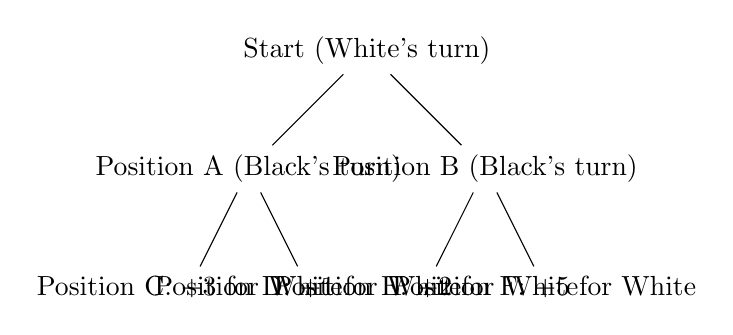
\begin{tikzpicture}[level distance=1.5cm,
  level 1/.style={sibling distance=3cm},
  level 2/.style={sibling distance=1.5cm}]
  \node {Start (White's turn)}
    child {node {Position A (Black's turn)}
      child {node {Position C: +3 for White}}
      child {node {Position D: +1 for White}}
    }
    child {node {Position B (Black's turn)}
      child {node {Position E: +2 for White}}
      child {node {Position F: +5 for White}}
    };
\end{tikzpicture}
\end{center}

In this example:
\begin{itemize}
    \item White has two possible moves from the start position, leading to positions A or B
    \item From position A, Black has two possible moves, leading to positions C or D
    \item From position B, Black has two possible moves, leading to positions E or F
    \item The numbers at the bottom are the evaluations (higher is better for White)
\end{itemize}

Using Minimax:
\begin{enumerate}
    \item If White chooses move A, Black will choose the move leading to position D (since +1 is worse for White than +3)
    \item If White chooses move B, Black will choose the move leading to position E (since +2 is worse for White than +5)
    \item So White's choices are effectively between positions D (+1) and E (+2)
    \item White will choose move B, leading to position E with a value of +2
\end{enumerate}

\subsubsection{Minimax with Depth}

The example above only looked one move ahead. In real chess, we want to look many moves ahead. We do this by applying Minimax recursively to a certain depth.

For example, if we set depth=4, the computer will look ahead 4 moves (2 moves by each player). The deeper we go, the better the computer will play, but the more calculations it needs to do.

\subsubsection{The Problem with Minimax}

The main problem with Minimax is that it grows exponentially with depth. In chess, each position has about 35 possible moves on average. So:
\begin{itemize}
    \item At depth 1: 35 positions to evaluate
    \item At depth 2: 35 × 35 = 1,225 positions
    \item At depth 3: 35 × 35 × 35 = 42,875 positions
    \item At depth 4: 35 × 35 × 35 × 35 = 1,500,625 positions
\end{itemize}

This quickly becomes too much for even the fastest computers. That's why we need more efficient algorithms, which we'll explore next.

\subsection{Alpha-Beta Pruning}

To make Minimax more efficient, we can use a technique called Alpha-Beta Pruning. This doesn't change the final decision, but it allows us to skip evaluating many positions that won't affect the outcome.

\subsubsection{How Alpha-Beta Pruning Works}

The key insight of Alpha-Beta Pruning is that once we find a good move, we can ignore moves that are clearly worse without fully evaluating them.

Let's go back to our example:

\begin{center}
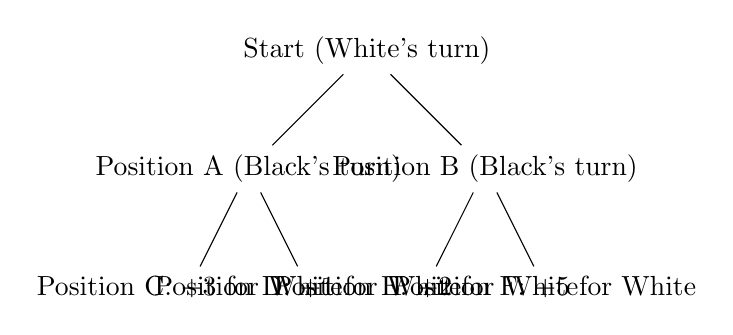
\begin{tikzpicture}[level distance=1.5cm,
  level 1/.style={sibling distance=3cm},
  level 2/.style={sibling distance=1.5cm}]
  \node {Start (White's turn)}
    child {node {Position A (Black's turn)}
      child {node {Position C: +3 for White}}
      child {node {Position D: +1 for White}}
    }
    child {node {Position B (Black's turn)}
      child {node {Position E: +2 for White}}
      child {node {Position F: +5 for White}}
    };
\end{tikzpicture}
\end{center}

With Alpha-Beta Pruning:
\begin{enumerate}
    \item White first explores move A
    \item Black's best response is move D, with value +1
    \item White then explores move B
    \item Black's first option is move E, with value +2
    \item Since +2 is already better than +1, White knows that move B is better than move A
    \item White doesn't need to explore Black's second option (move F) at all!
\end{enumerate}

In a real chess game with billions of possible positions, Alpha-Beta Pruning can eliminate huge portions of the search tree, allowing the computer to look much deeper in the same amount of time.

\subsubsection{Alpha-Beta Pruning in Code}

Here's a simplified version of how Alpha-Beta Pruning might be implemented in Python:

\begin{lstlisting}[style=Python]
def alpha_beta(position, depth, alpha, beta, maximizing_player):
    if depth == 0 or game_over(position):
        return evaluate(position)

    if maximizing_player:
        max_eval = float('-inf')
        for move in get_possible_moves(position):
            new_position = make_move(position, move)
            eval = alpha_beta(new_position, depth-1, alpha, beta, False)
            max_eval = max(max_eval, eval)
            alpha = max(alpha, eval)
            if beta <= alpha:
                break  # Beta cutoff
        return max_eval
    else:
        min_eval = float('inf')
        for move in get_possible_moves(position):
            new_position = make_move(position, move)
            eval = alpha_beta(new_position, depth-1, alpha, beta, True)
            min_eval = min(min_eval, eval)
            beta = min(beta, eval)
            if beta <= alpha:
                break  # Alpha cutoff
        return min_eval
\end{lstlisting}

The key part is the `if beta <= alpha: break` line, which is where we "prune" branches that won't affect the final decision.

\subsection{Monte Carlo Tree Search}

While Minimax with Alpha-Beta Pruning was the dominant approach in chess AI for decades, a newer algorithm called Monte Carlo Tree Search (MCTS) has become popular in recent years, especially for games like Go.

\subsubsection{How MCTS Works}

MCTS is based on random sampling. Instead of trying to evaluate every possible move, it plays many random games (simulations) from the current position and keeps track of which moves tend to lead to wins.

The algorithm has four main steps:
\begin{enumerate}
    \item \textbf{Selection}: Start from the root (current position) and select successive child nodes until reaching a leaf node. The selection is based on a formula that balances exploration (trying new moves) and exploitation (focusing on promising moves).

    \item \textbf{Expansion}: If the leaf node is not a terminal state (end of game), create one or more child nodes and select one.

    \item \textbf{Simulation}: Play a random game from the selected node until reaching a terminal state.

    \item \textbf{Backpropagation}: Update the statistics of all nodes in the path from the selected node to the root based on the result of the simulation.
\end{enumerate}

\subsubsection{MCTS Example}

Let's see a simple example of how MCTS might work in a chess-like game:

\begin{enumerate}
    \item We start at the current position and have three possible moves: A, B, and C.

    \item We haven't tried any of them yet, so we select move A (randomly).

    \item From position A, we play a random game until someone wins. Let's say White wins.

    \item We update the statistics for move A: 1 win out of 1 game.

    \item Next iteration, we select move B (to explore all options).

    \item From position B, we play a random game. Let's say Black wins.

    \item We update the statistics for move B: 0 wins out of 1 game.

    \item Next iteration, we select move C.

    \item From position C, we play a random game. Let's say White wins.

    \item We update the statistics for move C: 1 win out of 1 game.

    \item Now all moves have been tried once. In future iterations, we'll select based on which moves have the highest win rate, but also occasionally try moves with lower win rates (to make sure we don't miss anything).
\end{enumerate}

After many iterations (thousands or millions), we'll have a good estimate of which move is best.

\subsubsection{MCTS vs. Minimax}

MCTS has several advantages over Minimax:
\begin{itemize}
    \item It doesn't need an evaluation function (it just needs to know who won the game)
    \item It can be stopped at any time and will still give a reasonable move
    \item It naturally focuses on the most promising variations
    \item It handles uncertainty and randomness well
\end{itemize}

However, MCTS also has disadvantages:
\begin{itemize}
    \item It can miss tactical opportunities that Minimax would find
    \item It requires many simulations to be effective
    \item In games with a high branching factor (like chess), the random simulations might not be very informative
\end{itemize}

\subsubsection{MCTS in Code}

Here's a simplified version of how MCTS might be implemented in Python:

\begin{lstlisting}[style=Python]
import math
import random

class Node:
    def __init__(self, state, parent=None, move=None):
        self.state = state
        self.parent = parent
        self.move = move
        self.children = []
        self.wins = 0
        self.visits = 0
        self.untried_moves = get_possible_moves(state)

    def select_child(self):
        # UCB1 formula for selection
        s = sorted(self.children, key=lambda c: c.wins/c.visits +
                  math.sqrt(2*math.log(self.visits)/c.visits))
        return s[-1]  # Return the child with the highest UCB1 value

    def expand(self):
        move = self.untried_moves.pop()
        new_state = make_move(self.state, move)
        child = Node(new_state, self, move)
        self.children.append(child)
        return child

    def update(self, result):
        self.visits += 1
        self.wins += result

def monte_carlo_tree_search(root_state, iterations):
    root = Node(root_state)

    for _ in range(iterations):
        # Selection
        node = root
        while node.untried_moves == [] and node.children != []:
            node = node.select_child()

        # Expansion
        if node.untried_moves != []:
            node = node.expand()

        # Simulation
        state = node.state
        while not game_over(state):
            moves = get_possible_moves(state)
            move = random.choice(moves)
            state = make_move(state, move)

        # Backpropagation
        result = 1 if white_wins(state) else 0
        while node is not None:
            node.update(result)
            node = node.parent

    # Return the move with the highest number of visits
    return sorted(root.children, key=lambda c: c.visits)[-1].move
\end{lstlisting}

This is a basic implementation of MCTS. In practice, there are many optimizations and variations of this algorithm.

\section{Machine Learning for Chess}

So far, we've looked at traditional algorithms where humans explicitly program the rules for how the computer should play chess. Now, let's explore how computers can learn to play chess on their own through machine learning.

\subsection{From Handcrafted Rules to Learning}

Traditional chess engines like Stockfish use handcrafted evaluation functions created by chess experts. These functions consider factors like piece values, king safety, pawn structure, etc. While effective, creating and tuning these functions requires a lot of human expertise.

Machine learning takes a different approach: instead of telling the computer exactly how to evaluate positions, we let it learn from data. This has several advantages:
\begin{itemize}
    \item The computer might discover patterns that humans haven't noticed
    \item The evaluation can be more nuanced and adapt to different styles of play
    \item We don't need chess experts to create the evaluation function
\end{itemize}

\subsection{Neural Networks}

The most common type of machine learning model used in modern chess AI is the neural network. Neural networks are loosely inspired by how the human brain works, with interconnected "neurons" that process information.

\subsubsection{How Neural Networks Work}

A neural network consists of layers of neurons:
\begin{itemize}
    \item \textbf{Input Layer}: Receives the initial data (in chess, this would be the board position)
    \item \textbf{Hidden Layers}: Process the information through a series of mathematical operations
    \item \textbf{Output Layer}: Produces the final result (in chess, this might be an evaluation of the position or a probability distribution over possible moves)
\end{itemize}

Each neuron takes inputs from the previous layer, applies weights to them, sums them up, and then applies an "activation function" to produce its output. The weights are what the network learns during training.

\subsubsection{Neural Network Example}

Here's a simple example of how a neural network might evaluate a chess position:

\begin{enumerate}
    \item \textbf{Input}: The board position, represented as a 64-element array (one for each square), where each element indicates what piece (if any) is on that square.

    \item \textbf{Hidden Layer 1}: Might learn to recognize patterns like "knight fork" or "queen in danger."

    \item \textbf{Hidden Layer 2}: Might combine these patterns to understand concepts like "attacking position" or "defensive structure."

    \item \textbf{Output}: A single number representing the evaluation of the position (positive for White advantage, negative for Black advantage).
\end{enumerate}

\subsubsection{Training Neural Networks}

Neural networks learn by adjusting their weights based on examples. For chess, we might train a network by:
\begin{itemize}
    \item Showing it millions of positions from real games
    \item For each position, telling it who eventually won the game
    \item Adjusting the weights so that the network's evaluation better predicts the winner
\end{itemize}

This process is called "supervised learning" because we're supervising the network by providing the correct answers.

\subsection{Reinforcement Learning}

While supervised learning is powerful, it requires a large dataset of labeled examples. Reinforcement learning (RL) is another approach where the computer learns by playing against itself and receiving rewards for good moves.

\subsubsection{How Reinforcement Learning Works}

In reinforcement learning:
\begin{enumerate}
    \item The agent (our chess AI) observes the current state (the board position)
    \item It takes an action (makes a move)
    \item It receives a reward (e.g., +1 for winning, -1 for losing, 0 for drawing)
    \item It updates its policy (strategy for choosing moves) to maximize future rewards
\end{enumerate}

The key insight is that the agent doesn't need to be told exactly what to do in each situation. It learns through trial and error, gradually improving its policy.

\subsubsection{Policy and Value Functions}

In reinforcement learning for chess, we typically have two main components:
\begin{itemize}
    \item \textbf{Policy Function}: Decides which move to make in a given position
    \item \textbf{Value Function}: Estimates how good a position is
\end{itemize}

Both of these can be represented by neural networks:
\begin{itemize}
    \item The policy network takes a board position as input and outputs a probability distribution over possible moves
    \item The value network takes a board position as input and outputs an estimate of who will win from that position
\end{itemize}

\subsubsection{Self-Play}

One of the most effective ways to train a reinforcement learning agent for chess is through self-play:
\begin{enumerate}
    \item Start with a randomly initialized policy
    \item Have the agent play games against itself
    \item Use the outcomes of these games to improve the policy
    \item Repeat with the improved policy
\end{enumerate}

This approach was used by AlphaZero, a chess AI developed by DeepMind that famously defeated Stockfish (one of the strongest traditional chess engines) after learning to play chess in just 24 hours of self-play.

\section{Deep Reinforcement Learning}
\subsection{PPO Algorithm: From Basics to Advanced}

\subsubsection{Understanding Reinforcement Learning Basics}

Before diving into PPO, let's understand the basic reinforcement learning concepts. Imagine you're teaching a child to play chess:

\begin{enumerate}
    \item The child looks at the chess board (this is the \textbf{state} $s$)
    \item The child makes a move (this is the \textbf{action} $a$)
    \item You tell them if the move was good or bad (this is the \textbf{reward} $r$)
    \item The board changes to a new position (this is the \textbf{next state} $s'$)
    \item This process repeats until the game ends
\end{enumerate}

In mathematical terms, at each timestep $t$, the agent:
\begin{itemize}
    \item Observes state $s_t$
    \item Takes action $a_t$
    \item Receives reward $r_t$
    \item Transitions to state $s_{t+1}$
\end{itemize}

The goal is to find a policy $\pi(a|s)$ that maximizes the expected cumulative reward:

\begin{equation}
    J(\pi) = \mathbb{E}_{\tau \sim \pi} \left[ \sum_{t=0}^{T} \gamma^t r_t \right]
\end{equation}

Where:
\begin{itemize}
    \item $\pi(a|s)$ is our policy - it tells us the probability of taking action $a$ in state $s$
    \item $\tau$ is a trajectory (a complete sequence of states, actions, and rewards)
    \item $\gamma$ is a discount factor (value between 0 and 1) that makes future rewards worth less than immediate rewards
    \item $r_t$ is the reward at time step $t$
    \item $T$ is the time horizon (length of the game)
    \item $\mathbb{E}_{\tau \sim \pi}$ means the expected value over all possible trajectories when following policy $\pi$
\end{itemize}

\subsubsection*{Example with Chess}
Imagine a simple chess scenario:
\begin{itemize}
    \item You capture an opponent's pawn (+1 reward)
    \item Two moves later, you capture a knight (+3 reward)
    \item Three moves after that, you capture the queen (+9 reward)
    \item Finally, after two more moves, you checkmate (+50 reward)
\end{itemize}

With a discount factor $\gamma = 0.9$, your cumulative discounted reward would be:
\begin{align*}
    J &= 1 + 0.9^2 \times 3 + 0.9^5 \times 9 + 0.9^7 \times 50 \\
    &= 1 + 0.81 \times 3 + 0.59049 \times 9 + 0.47829 \times 50 \\
    &= 1 + 2.43 + 5.31 + 23.91 \\
    &= 32.65
\end{align*}

If we didn't use discounting ($\gamma = 1$), the sum would simply be $1 + 3 + 9 + 50 = 63$. The discounting makes immediate rewards more valuable than delayed rewards, encouraging the agent to achieve goals sooner rather than later.

\subsubsection{Value Functions and Advantages}

We use two important functions in reinforcement learning:
\begin{itemize}
    \item \textbf{Value function} $V^\pi(s)$: How good is it to be in state $s$? This estimates the total expected future reward from being in state $s$ and following policy $\pi$ afterward.
    \item \textbf{Q-function} $Q^\pi(s,a)$: How good is it to take action $a$ in state $s$? This estimates the total expected future reward from taking action $a$ in state $s$ and then following policy $\pi$ afterward.
\end{itemize}

Mathematically:
\begin{equation}
    V^\pi(s) = \mathbb{E}_{\tau \sim \pi} \left[ \sum_{t=0}^{T} \gamma^t r_t | s_0 = s \right]
\end{equation}

This equation means: "What's the expected total reward if I start in state $s$ and follow policy $\pi$ all the way to the end of the game?"

\begin{equation}
    Q^\pi(s,a) = \mathbb{E}_{\tau \sim \pi} \left[ \sum_{t=0}^{T} \gamma^t r_t | s_0 = s, a_0 = a \right]
\end{equation}

This equation means: "What's the expected total reward if I take action $a$ in state $s$ right now, and then follow policy $\pi$ all the way to the end of the game?"

\subsubsection*{Chess Example for Value Function}
Imagine you're evaluating a chess position:
\begin{itemize}
    \item Position A: You have a queen advantage, and your opponent's king is exposed. Value function might estimate: $V(\text{Position A}) = +8$ (very good for you)
    \item Position B: Equal material, but your pieces are poorly positioned. Value function might estimate: $V(\text{Position B}) = -1$ (slightly bad for you)
\end{itemize}

\subsubsection*{Chess Example for Q-Function}
For a given position, different moves have different Q-values:
\begin{itemize}
    \item Move 1: Capture opponent's queen with your knight. $Q(\text{Position}, \text{Capture Queen}) = +7$ (excellent move)
    \item Move 2: Move your pawn forward one square. $Q(\text{Position}, \text{Advance Pawn}) = +0.5$ (slightly good move)
    \item Move 3: Move your king into check. $Q(\text{Position}, \text{King into Check}) = -10$ (terrible move)
\end{itemize}

The \textbf{advantage function} tells us how much better an action is compared to the average action:
\begin{equation}
    A^\pi(s,a) = Q^\pi(s,a) - V^\pi(s)
\end{equation}

This is extremely important because it tells us which actions are better than the average action in a given state. It's the key to learning which actions to prefer.

\subsubsection*{Chess Example for Advantage Function}
Imagine a position where the overall value is $V(\text{Position}) = +2$ (slightly good for you). For different moves:
\begin{itemize}
    \item Move 1: Capture opponent's queen. $Q(\text{Position}, \text{Capture Queen}) = +9$
    $\Rightarrow$ Advantage = $Q(\text{Position}, \text{Capture Queen}) - V(\text{Position}) = +9 - (+2) = +7$ (much better than average)
    
    \item Move 2: Move pawn forward. $Q(\text{Position}, \text{Advance Pawn}) = +2$
    $\Rightarrow$ Advantage = $Q(\text{Position}, \text{Advance Pawn}) - V(\text{Position}) = +2 - (+2) = 0$ (exactly average)
    
    \item Move 3: Blunder your bishop. $Q(\text{Position}, \text{Blunder Bishop}) = -3$
    $\Rightarrow$ Advantage = $Q(\text{Position}, \text{Blunder Bishop}) - V(\text{Position}) = -3 - (+2) = -5$ (much worse than average)
\end{itemize}

The agent will learn to prefer actions with positive advantage and avoid actions with negative advantage.

\subsubsection{From Basic RL to PPO}

Proximal Policy Optimization (PPO) is an advanced reinforcement learning algorithm that makes learning more stable and efficient. Imagine PPO as a smart robot learning to play chess. Let's break it down into simple parts:

\begin{figure}[h]
    \centering
    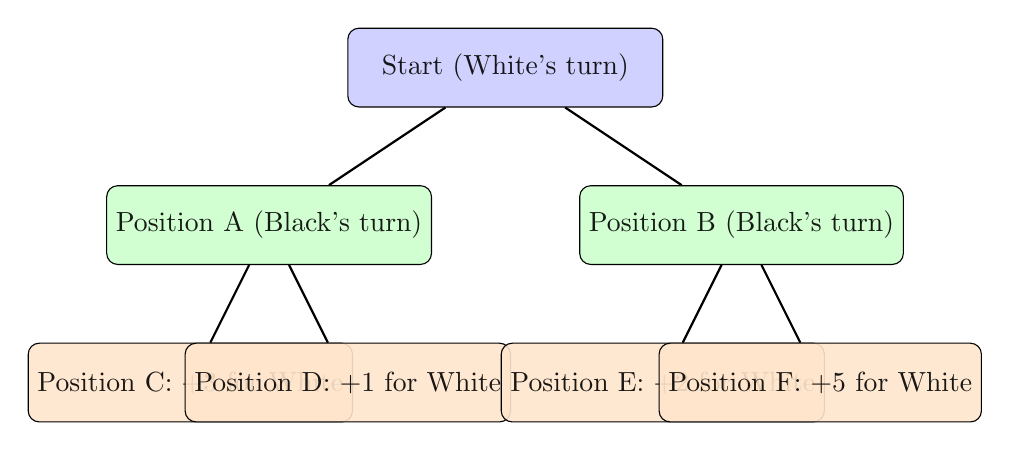
\begin{tikzpicture}[
        scale=1.0,
        transform shape,
        level distance=2cm,
        sibling distance=3cm,
        every node/.style={draw, rectangle, rounded corners, minimum width=4cm, minimum height=1cm, align=center, fill opacity=0.9}
    ]
        % Root node
        \node[fill=blue!20] (root) at (0,0) {Start (White's turn)};
        
        % Level 1 nodes
        \node[fill=green!20] (A) at (-3,-2) {Position A (Black's turn)};
        \node[fill=green!20] (B) at (3,-2) {Position B (Black's turn)};
        
        % Level 2 nodes
        \node[fill=orange!20] (C) at (-4,-4) {Position C: +3 for White};
        \node[fill=orange!20] (D) at (-2,-4) {Position D: +1 for White};
        \node[fill=orange!20] (E) at (2,-4) {Position E: +2 for White};
        \node[fill=orange!20] (F) at (4,-4) {Position F: +5 for White};
        
        % Connect nodes
        \draw[thick] (root) -- (A);
        \draw[thick] (root) -- (B);
        \draw[thick] (A) -- (C);
        \draw[thick] (A) -- (D);
        \draw[thick] (B) -- (E);
        \draw[thick] (B) -- (F);
    \end{tikzpicture}
    \caption{Minimax example with improved spacing and layout}
    \label{fig:minimax_example}
\end{figure}

\begin{figure}[ht]
    \centering
    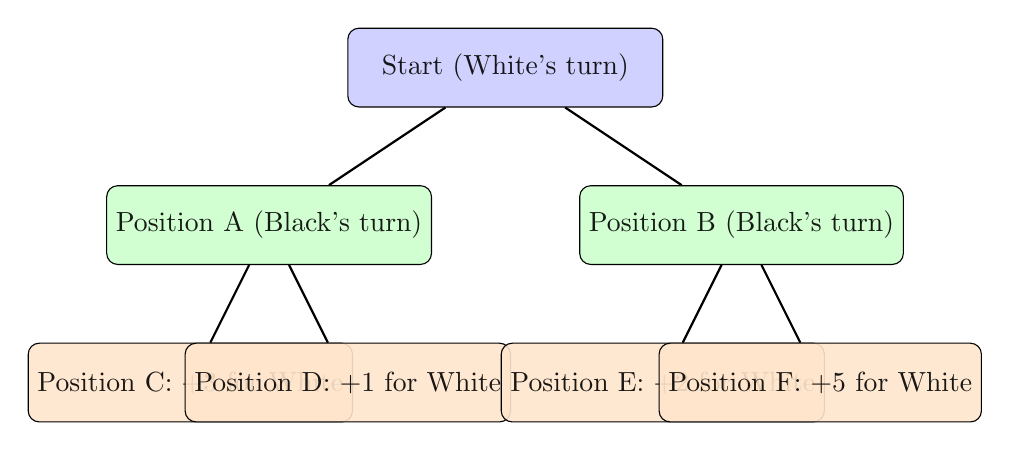
\begin{tikzpicture}[
        scale=1.0,
        transform shape,
        level distance=2cm,
        sibling distance=3cm,
        every node/.style={draw, rectangle, rounded corners, minimum width=4cm, minimum height=1cm, align=center, fill opacity=0.9}
    ]
        % Root node
        \node[fill=blue!20] (root) at (0,0) {Start (White's turn)};
        
        % Level 1 nodes
        \node[fill=green!20] (A) at (-3,-2) {Position A (Black's turn)};
        \node[fill=green!20] (B) at (3,-2) {Position B (Black's turn)};
        
        % Level 2 nodes
        \node[fill=orange!20] (C) at (-4,-4) {Position C: +3 for White};
        \node[fill=orange!20] (D) at (-2,-4) {Position D: +1 for White};
        \node[fill=orange!20] (E) at (2,-4) {Position E: +2 for White};
        \node[fill=orange!20] (F) at (4,-4) {Position F: +5 for White};
        
        % Connect nodes
        \draw[thick] (root) -- (A);
        \draw[thick] (root) -- (B);
        \draw[thick] (A) -- (C);
        \draw[thick] (A) -- (D);
        \draw[thick] (B) -- (E);
        \draw[thick] (B) -- (F);
    \end{tikzpicture}
    \caption{Minimax example with improved spacing and layout}
    \label{fig:minimax_example}
\end{figure}

\begin{figure}[ht]
    \centering
    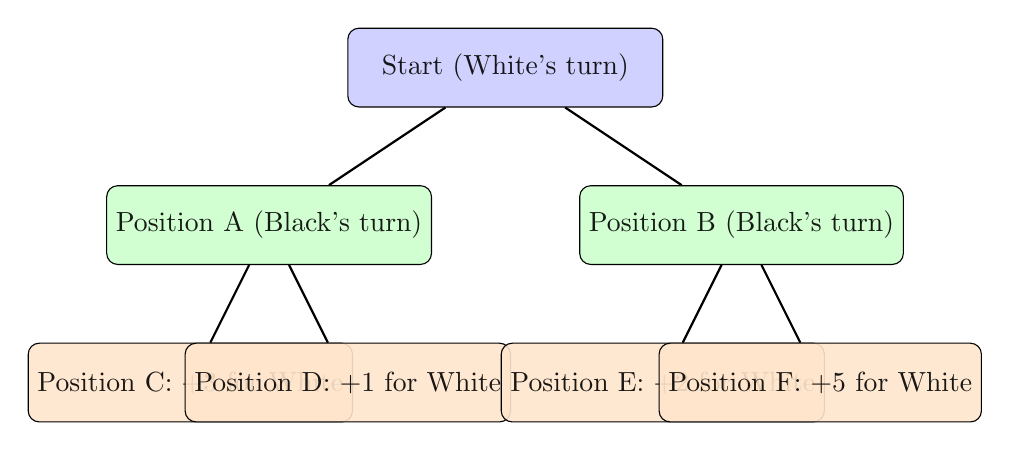
\begin{tikzpicture}[
        scale=1.0,
        transform shape,
        level distance=2cm,
        sibling distance=3cm,
        every node/.style={draw, rectangle, rounded corners, minimum width=4cm, minimum height=1cm, align=center, fill opacity=0.9}
    ]
        % Root node
        \node[fill=blue!20] (root) at (0,0) {Start (White's turn)};
        
        % Level 1 nodes
        \node[fill=green!20] (A) at (-3,-2) {Position A (Black's turn)};
        \node[fill=green!20] (B) at (3,-2) {Position B (Black's turn)};
        
        % Level 2 nodes
        \node[fill=orange!20] (C) at (-4,-4) {Position C: +3 for White};
        \node[fill=orange!20] (D) at (-2,-4) {Position D: +1 for White};
        \node[fill=orange!20] (E) at (2,-4) {Position E: +2 for White};
        \node[fill=orange!20] (F) at (4,-4) {Position F: +5 for White};
        
        % Connect nodes
        \draw[thick] (root) -- (A);
        \draw[thick] (root) -- (B);
        \draw[thick] (A) -- (C);
        \draw[thick] (A) -- (D);
        \draw[thick] (B) -- (E);
        \draw[thick] (B) -- (F);
    \end{tikzpicture}
    \caption{Minimax example with improved spacing and layout}
    \label{fig:minimax_example}
\end{figure}

\begin{figure}[ht]
    \centering
    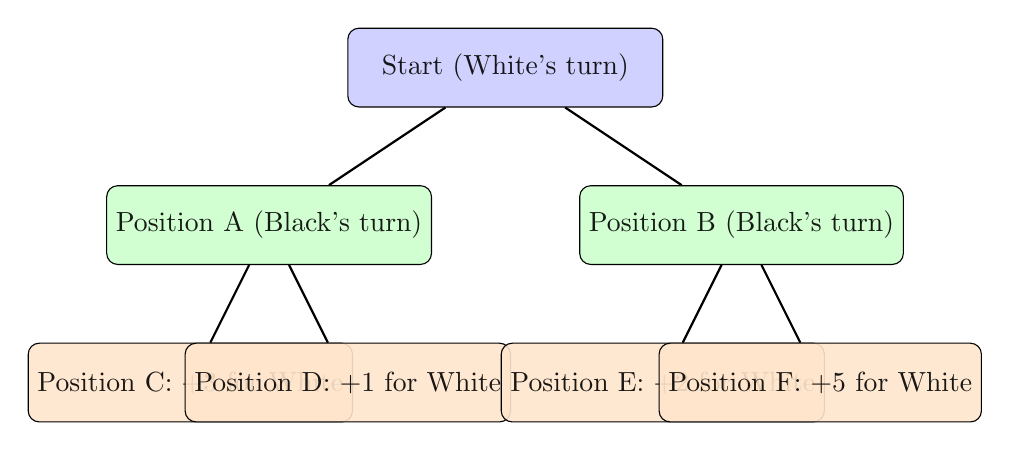
\begin{tikzpicture}[
        scale=1.0,
        transform shape,
        level distance=2cm,
        sibling distance=3cm,
        every node/.style={draw, rectangle, rounded corners, minimum width=4cm, minimum height=1cm, align=center, fill opacity=0.9}
    ]
        % Root node
        \node[fill=blue!20] (root) at (0,0) {Start (White's turn)};
        
        % Level 1 nodes
        \node[fill=green!20] (A) at (-3,-2) {Position A (Black's turn)};
        \node[fill=green!20] (B) at (3,-2) {Position B (Black's turn)};
        
        % Level 2 nodes
        \node[fill=orange!20] (C) at (-4,-4) {Position C: +3 for White};
        \node[fill=orange!20] (D) at (-2,-4) {Position D: +1 for White};
        \node[fill=orange!20] (E) at (2,-4) {Position E: +2 for White};
        \node[fill=orange!20] (F) at (4,-4) {Position F: +5 for White};
        
        % Connect nodes
        \draw[thick] (root) -- (A);
        \draw[thick] (root) -- (B);
        \draw[thick] (A) -- (C);
        \draw[thick] (A) -- (D);
        \draw[thick] (B) -- (E);
        \draw[thick] (B) -- (F);
    \end{tikzpicture}
    \caption{Minimax example with improved spacing and layout}
    \label{fig:minimax_example}
\end{figure}

\begin{figure}[ht]
    \centering
    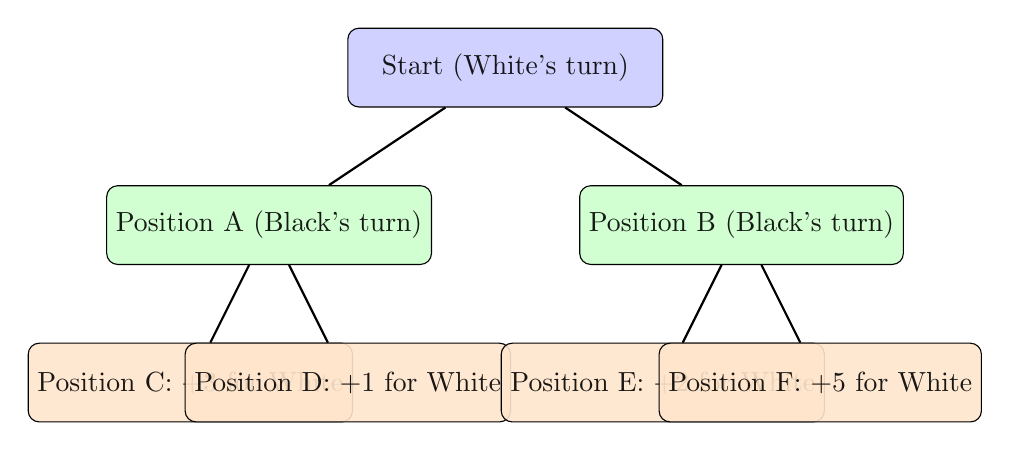
\begin{tikzpicture}[
        scale=1.0,
        transform shape,
        level distance=2cm,
        sibling distance=3cm,
        every node/.style={draw, rectangle, rounded corners, minimum width=4cm, minimum height=1cm, align=center, fill opacity=0.9}
    ]
        % Root node
        \node[fill=blue!20] (root) at (0,0) {Start (White's turn)};
        
        % Level 1 nodes
        \node[fill=green!20] (A) at (-3,-2) {Position A (Black's turn)};
        \node[fill=green!20] (B) at (3,-2) {Position B (Black's turn)};
        
        % Level 2 nodes
        \node[fill=orange!20] (C) at (-4,-4) {Position C: +3 for White};
        \node[fill=orange!20] (D) at (-2,-4) {Position D: +1 for White};
        \node[fill=orange!20] (E) at (2,-4) {Position E: +2 for White};
        \node[fill=orange!20] (F) at (4,-4) {Position F: +5 for White};
        
        % Connect nodes
        \draw[thick] (root) -- (A);
        \draw[thick] (root) -- (B);
        \draw[thick] (A) -- (C);
        \draw[thick] (A) -- (D);
        \draw[thick] (B) -- (E);
        \draw[thick] (B) -- (F);
    \end{tikzpicture}
    \caption{Minimax example with improved spacing and layout}
    \label{fig:minimax_example}
\end{figure}

\begin{figure}[ht]
    \centering
    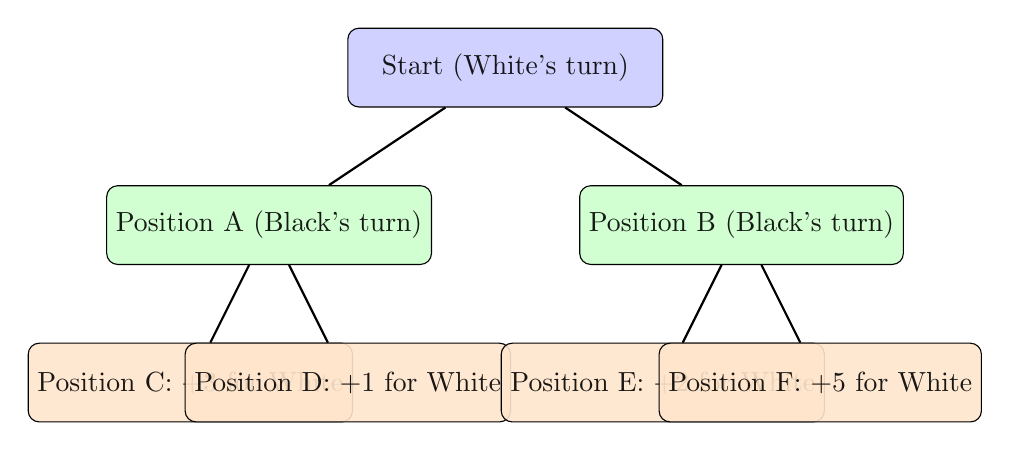
\begin{tikzpicture}[
        scale=1.0,
        transform shape,
        level distance=2cm,
        sibling distance=3cm,
        every node/.style={draw, rectangle, rounded corners, minimum width=4cm, minimum height=1cm, align=center, fill opacity=0.9}
    ]
        % Root node
        \node[fill=blue!20] (root) at (0,0) {Start (White's turn)};
        
        % Level 1 nodes
        \node[fill=green!20] (A) at (-3,-2) {Position A (Black's turn)};
        \node[fill=green!20] (B) at (3,-2) {Position B (Black's turn)};
        
        % Level 2 nodes
        \node[fill=orange!20] (C) at (-4,-4) {Position C: +3 for White};
        \node[fill=orange!20] (D) at (-2,-4) {Position D: +1 for White};
        \node[fill=orange!20] (E) at (2,-4) {Position E: +2 for White};
        \node[fill=orange!20] (F) at (4,-4) {Position F: +5 for White};
        
        % Connect nodes
        \draw[thick] (root) -- (A);
        \draw[thick] (root) -- (B);
        \draw[thick] (A) -- (C);
        \draw[thick] (A) -- (D);
        \draw[thick] (B) -- (E);
        \draw[thick] (B) -- (F);
    \end{tikzpicture}
    \caption{Minimax example with improved spacing and layout}
    \label{fig:minimax_example}
\end{figure}

\begin{figure}[ht]
    \centering
    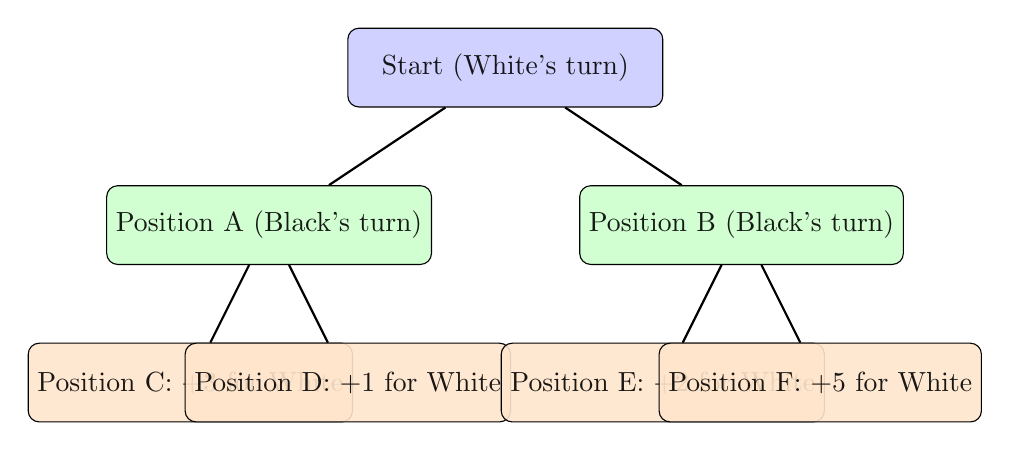
\begin{tikzpicture}[
        scale=1.0,
        transform shape,
        level distance=2cm,
        sibling distance=3cm,
        every node/.style={draw, rectangle, rounded corners, minimum width=4cm, minimum height=1cm, align=center, fill opacity=0.9}
    ]
        % Root node
        \node[fill=blue!20] (root) at (0,0) {Start (White's turn)};
        
        % Level 1 nodes
        \node[fill=green!20] (A) at (-3,-2) {Position A (Black's turn)};
        \node[fill=green!20] (B) at (3,-2) {Position B (Black's turn)};
        
        % Level 2 nodes
        \node[fill=orange!20] (C) at (-4,-4) {Position C: +3 for White};
        \node[fill=orange!20] (D) at (-2,-4) {Position D: +1 for White};
        \node[fill=orange!20] (E) at (2,-4) {Position E: +2 for White};
        \node[fill=orange!20] (F) at (4,-4) {Position F: +5 for White};
        
        % Connect nodes
        \draw[thick] (root) -- (A);
        \draw[thick] (root) -- (B);
        \draw[thick] (A) -- (C);
        \draw[thick] (A) -- (D);
        \draw[thick] (B) -- (E);
        \draw[thick] (B) -- (F);
    \end{tikzpicture}
    \caption{Minimax example with improved spacing and layout}
    \label{fig:minimax_example}
\end{figure}

\begin{figure}[ht]
    \centering
    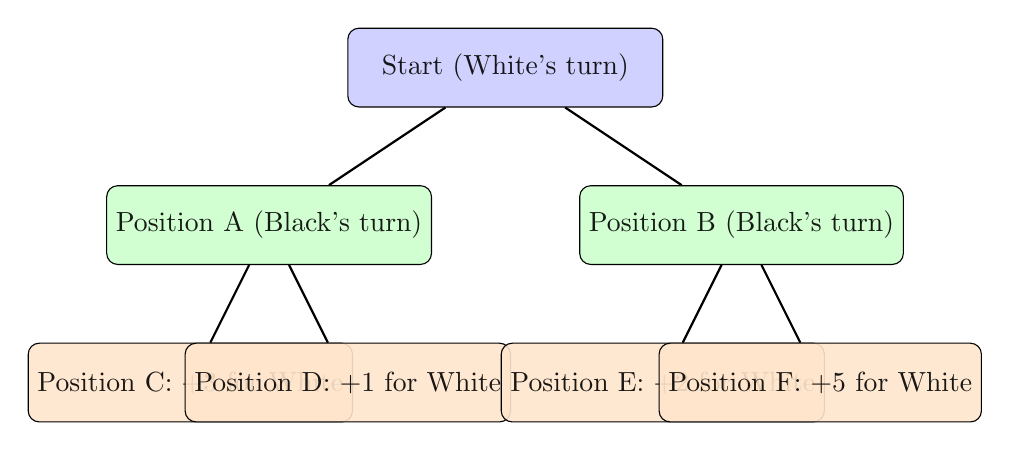
\begin{tikzpicture}[
        scale=1.0,
        transform shape,
        level distance=2cm,
        sibling distance=3cm,
        every node/.style={draw, rectangle, rounded corners, minimum width=4cm, minimum height=1cm, align=center, fill opacity=0.9}
    ]
        % Root node
        \node[fill=blue!20] (root) at (0,0) {Start (White's turn)};
        
        % Level 1 nodes
        \node[fill=green!20] (A) at (-3,-2) {Position A (Black's turn)};
        \node[fill=green!20] (B) at (3,-2) {Position B (Black's turn)};
        
        % Level 2 nodes
        \node[fill=orange!20] (C) at (-4,-4) {Position C: +3 for White};
        \node[fill=orange!20] (D) at (-2,-4) {Position D: +1 for White};
        \node[fill=orange!20] (E) at (2,-4) {Position E: +2 for White};
        \node[fill=orange!20] (F) at (4,-4) {Position F: +5 for White};
        
        % Connect nodes
        \draw[thick] (root) -- (A);
        \draw[thick] (root) -- (B);
        \draw[thick] (A) -- (C);
        \draw[thick] (A) -- (D);
        \draw[thick] (B) -- (E);
        \draw[thick] (B) -- (F);
    \end{tikzpicture}
    \caption{Minimax example with improved spacing and layout}
    \label{fig:minimax_example}
\end{figure}

\begin{figure}[ht]
    \centering
    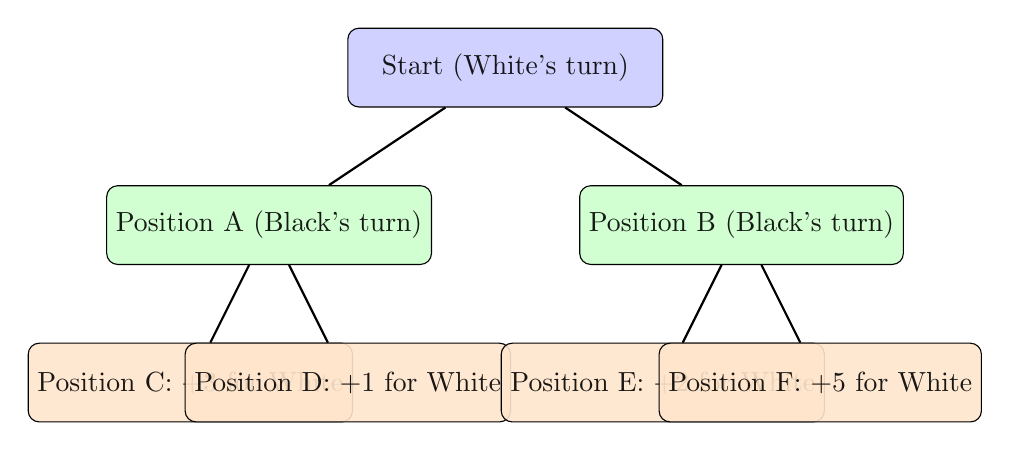
\begin{tikzpicture}[
        scale=1.0,
        transform shape,
        level distance=2cm,
        sibling distance=3cm,
        every node/.style={draw, rectangle, rounded corners, minimum width=4cm, minimum height=1cm, align=center, fill opacity=0.9}
    ]
        % Root node
        \node[fill=blue!20] (root) at (0,0) {Start (White's turn)};
        
        % Level 1 nodes
        \node[fill=green!20] (A) at (-3,-2) {Position A (Black's turn)};
        \node[fill=green!20] (B) at (3,-2) {Position B (Black's turn)};
        
        % Level 2 nodes
        \node[fill=orange!20] (C) at (-4,-4) {Position C: +3 for White};
        \node[fill=orange!20] (D) at (-2,-4) {Position D: +1 for White};
        \node[fill=orange!20] (E) at (2,-4) {Position E: +2 for White};
        \node[fill=orange!20] (F) at (4,-4) {Position F: +5 for White};
        
        % Connect nodes
        \draw[thick] (root) -- (A);
        \draw[thick] (root) -- (B);
        \draw[thick] (A) -- (C);
        \draw[thick] (A) -- (D);
        \draw[thick] (B) -- (E);
        \draw[thick] (B) -- (F);
    \end{tikzpicture}
    \caption{Minimax example with improved spacing and layout}
    \label{fig:minimax_example}
\end{figure}

\begin{figure}[ht]
    \centering
    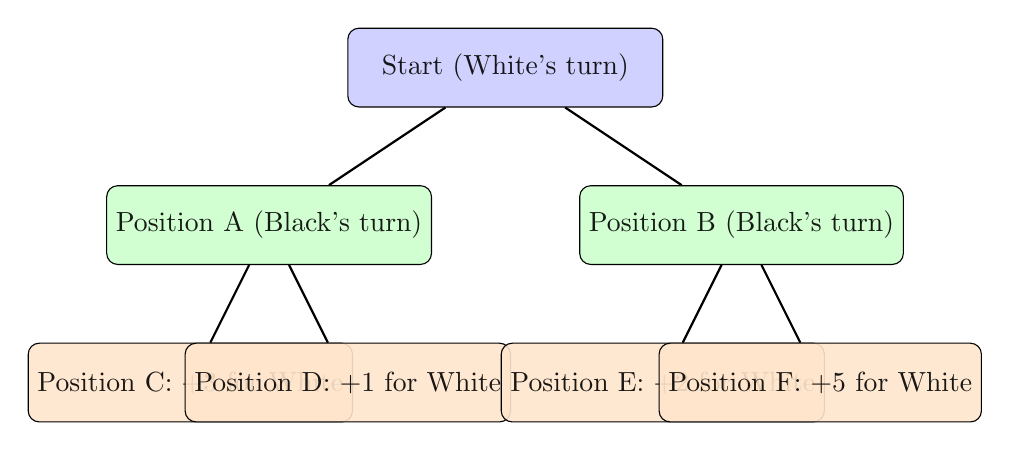
\begin{tikzpicture}[
        scale=1.0,
        transform shape,
        level distance=2cm,
        sibling distance=3cm,
        every node/.style={draw, rectangle, rounded corners, minimum width=4cm, minimum height=1cm, align=center, fill opacity=0.9}
    ]
        % Root node
        \node[fill=blue!20] (root) at (0,0) {Start (White's turn)};
        
        % Level 1 nodes
        \node[fill=green!20] (A) at (-3,-2) {Position A (Black's turn)};
        \node[fill=green!20] (B) at (3,-2) {Position B (Black's turn)};
        
        % Level 2 nodes
        \node[fill=orange!20] (C) at (-4,-4) {Position C: +3 for White};
        \node[fill=orange!20] (D) at (-2,-4) {Position D: +1 for White};
        \node[fill=orange!20] (E) at (2,-4) {Position E: +2 for White};
        \node[fill=orange!20] (F) at (4,-4) {Position F: +5 for White};
        
        % Connect nodes
        \draw[thick] (root) -- (A);
        \draw[thick] (root) -- (B);
        \draw[thick] (A) -- (C);
        \draw[thick] (A) -- (D);
        \draw[thick] (B) -- (E);
        \draw[thick] (B) -- (F);
    \end{tikzpicture}
    \caption{Minimax example with improved spacing and layout}
    \label{fig:minimax_example}
\end{figure}

\begin{figure}[ht]
    \centering
    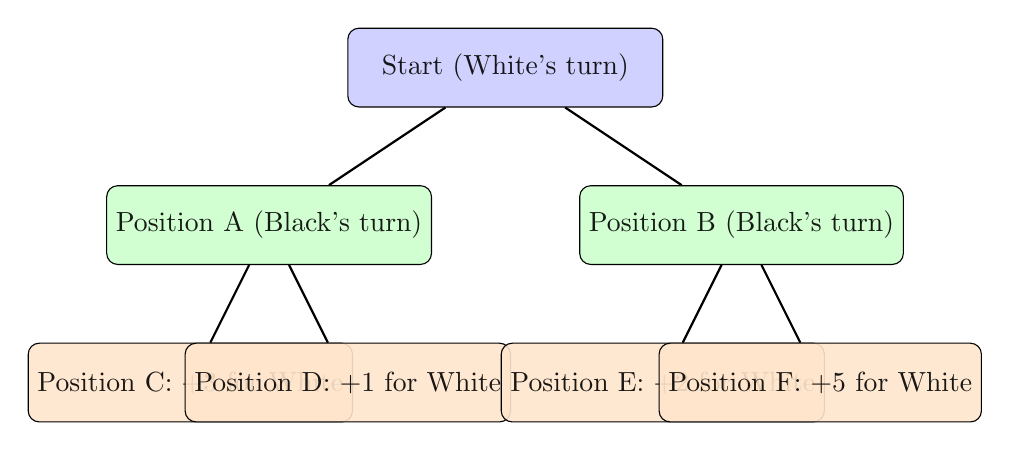
\begin{tikzpicture}[
        scale=1.0,
        transform shape,
        level distance=2cm,
        sibling distance=3cm,
        every node/.style={draw, rectangle, rounded corners, minimum width=4cm, minimum height=1cm, align=center, fill opacity=0.9}
    ]
        % Root node
        \node[fill=blue!20] (root) at (0,0) {Start (White's turn)};
        
        % Level 1 nodes
        \node[fill=green!20] (A) at (-3,-2) {Position A (Black's turn)};
        \node[fill=green!20] (B) at (3,-2) {Position B (Black's turn)};
        
        % Level 2 nodes
        \node[fill=orange!20] (C) at (-4,-4) {Position C: +3 for White};
        \node[fill=orange!20] (D) at (-2,-4) {Position D: +1 for White};
        \node[fill=orange!20] (E) at (2,-4) {Position E: +2 for White};
        \node[fill=orange!20] (F) at (4,-4) {Position F: +5 for White};
        
        % Connect nodes
        \draw[thick] (root) -- (A);
        \draw[thick] (root) -- (B);
        \draw[thick] (A) -- (C);
        \draw[thick] (A) -- (D);
        \draw[thick] (B) -- (E);
        \draw[thick] (B) -- (F);
    \end{tikzpicture}
    \caption{Minimax example with improved spacing and layout}
    \label{fig:minimax_example}
\end{figure}

\begin{figure}[ht]
    \centering
    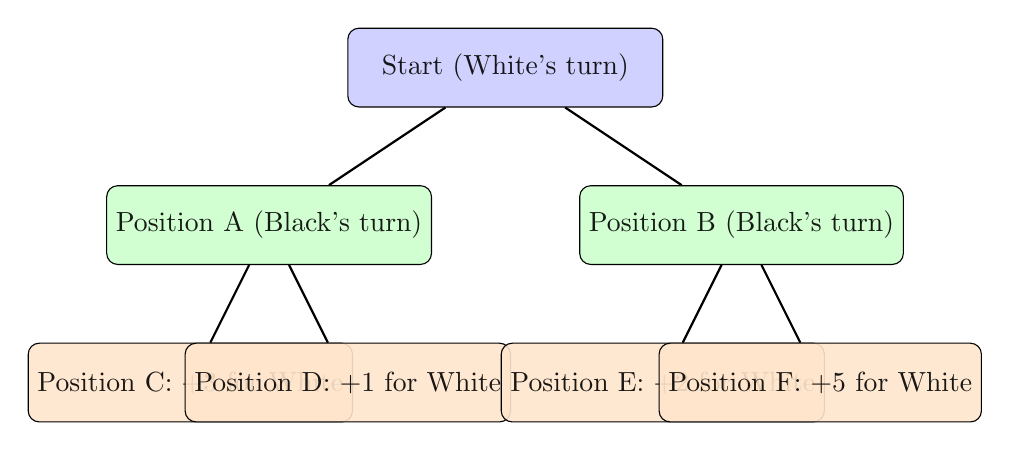
\begin{tikzpicture}[
        scale=1.0,
        transform shape,
        level distance=2cm,
        sibling distance=3cm,
        every node/.style={draw, rectangle, rounded corners, minimum width=4cm, minimum height=1cm, align=center, fill opacity=0.9}
    ]
        % Root node
        \node[fill=blue!20] (root) at (0,0) {Start (White's turn)};
        
        % Level 1 nodes
        \node[fill=green!20] (A) at (-3,-2) {Position A (Black's turn)};
        \node[fill=green!20] (B) at (3,-2) {Position B (Black's turn)};
        
        % Level 2 nodes
        \node[fill=orange!20] (C) at (-4,-4) {Position C: +3 for White};
        \node[fill=orange!20] (D) at (-2,-4) {Position D: +1 for White};
        \node[fill=orange!20] (E) at (2,-4) {Position E: +2 for White};
        \node[fill=orange!20] (F) at (4,-4) {Position F: +5 for White};
        
        % Connect nodes
        \draw[thick] (root) -- (A);
        \draw[thick] (root) -- (B);
        \draw[thick] (A) -- (C);
        \draw[thick] (A) -- (D);
        \draw[thick] (B) -- (E);
        \draw[thick] (B) -- (F);
    \end{tikzpicture}
    \caption{Minimax example with improved spacing and layout}
    \label{fig:minimax_example}
\end{figure}

\begin{figure}[ht]
    \centering
    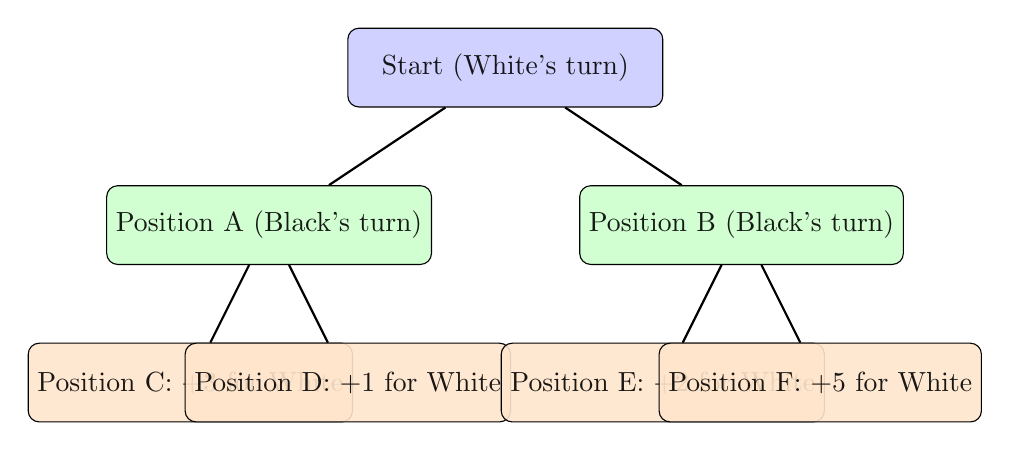
\begin{tikzpicture}[
        scale=1.0,
        transform shape,
        level distance=2cm,
        sibling distance=3cm,
        every node/.style={draw, rectangle, rounded corners, minimum width=4cm, minimum height=1cm, align=center, fill opacity=0.9}
    ]
        % Root node
        \node[fill=blue!20] (root) at (0,0) {Start (White's turn)};
        
        % Level 1 nodes
        \node[fill=green!20] (A) at (-3,-2) {Position A (Black's turn)};
        \node[fill=green!20] (B) at (3,-2) {Position B (Black's turn)};
        
        % Level 2 nodes
        \node[fill=orange!20] (C) at (-4,-4) {Position C: +3 for White};
        \node[fill=orange!20] (D) at (-2,-4) {Position D: +1 for White};
        \node[fill=orange!20] (E) at (2,-4) {Position E: +2 for White};
        \node[fill=orange!20] (F) at (4,-4) {Position F: +5 for White};
        
        % Connect nodes
        \draw[thick] (root) -- (A);
        \draw[thick] (root) -- (B);
        \draw[thick] (A) -- (C);
        \draw[thick] (A) -- (D);
        \draw[thick] (B) -- (E);
        \draw[thick] (B) -- (F);
    \end{tikzpicture}
    \caption{Minimax example with improved spacing and layout}
    \label{fig:minimax_example}
\end{figure}

\begin{figure}[ht]
    \centering
    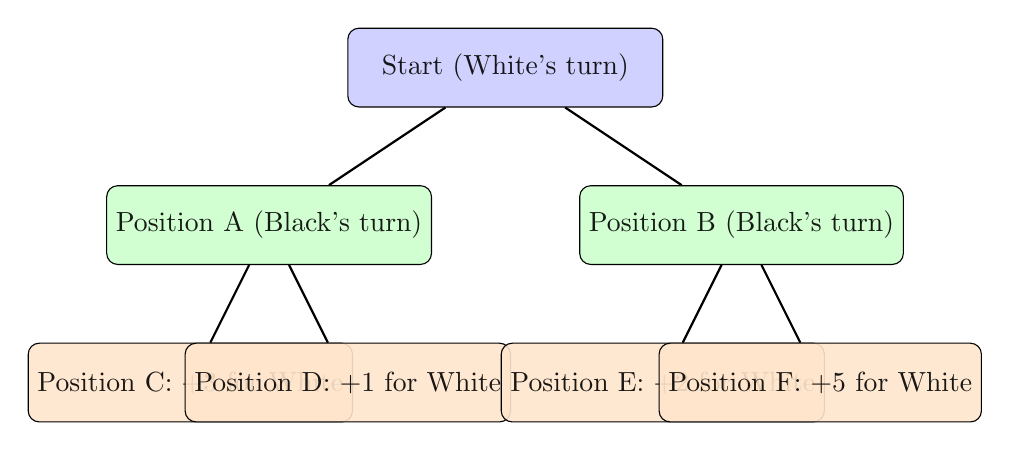
\begin{tikzpicture}[
        scale=1.0,
        transform shape,
        level distance=2cm,
        sibling distance=3cm,
        every node/.style={draw, rectangle, rounded corners, minimum width=4cm, minimum height=1cm, align=center, fill opacity=0.9}
    ]
        % Root node
        \node[fill=blue!20] (root) at (0,0) {Start (White's turn)};
        
        % Level 1 nodes
        \node[fill=green!20] (A) at (-3,-2) {Position A (Black's turn)};
        \node[fill=green!20] (B) at (3,-2) {Position B (Black's turn)};
        
        % Level 2 nodes
        \node[fill=orange!20] (C) at (-4,-4) {Position C: +3 for White};
        \node[fill=orange!20] (D) at (-2,-4) {Position D: +1 for White};
        \node[fill=orange!20] (E) at (2,-4) {Position E: +2 for White};
        \node[fill=orange!20] (F) at (4,-4) {Position F: +5 for White};
        
        % Connect nodes
        \draw[thick] (root) -- (A);
        \draw[thick] (root) -- (B);
        \draw[thick] (A) -- (C);
        \draw[thick] (A) -- (D);
        \draw[thick] (B) -- (E);
        \draw[thick] (B) -- (F);
    \end{tikzpicture}
    \caption{Minimax example with improved spacing and layout}
    \label{fig:minimax_example}
\end{figure}

\begin{figure}[ht]
    \centering
    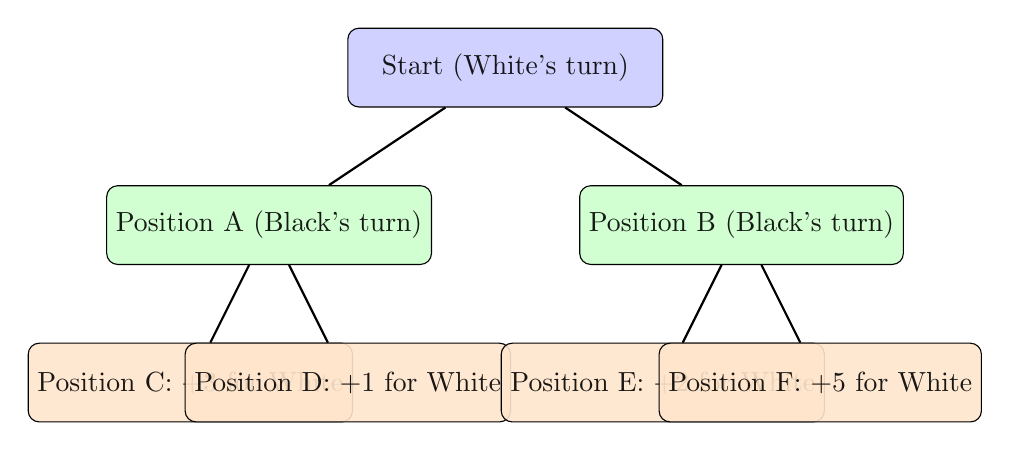
\begin{tikzpicture}[
        scale=1.0,
        transform shape,
        level distance=2cm,
        sibling distance=3cm,
        every node/.style={draw, rectangle, rounded corners, minimum width=4cm, minimum height=1cm, align=center, fill opacity=0.9}
    ]
        % Root node
        \node[fill=blue!20] (root) at (0,0) {Start (White's turn)};
        
        % Level 1 nodes
        \node[fill=green!20] (A) at (-3,-2) {Position A (Black's turn)};
        \node[fill=green!20] (B) at (3,-2) {Position B (Black's turn)};
        
        % Level 2 nodes
        \node[fill=orange!20] (C) at (-4,-4) {Position C: +3 for White};
        \node[fill=orange!20] (D) at (-2,-4) {Position D: +1 for White};
        \node[fill=orange!20] (E) at (2,-4) {Position E: +2 for White};
        \node[fill=orange!20] (F) at (4,-4) {Position F: +5 for White};
        
        % Connect nodes
        \draw[thick] (root) -- (A);
        \draw[thick] (root) -- (B);
        \draw[thick] (A) -- (C);
        \draw[thick] (A) -- (D);
        \draw[thick] (B) -- (E);
        \draw[thick] (B) -- (F);
    \end{tikzpicture}
    \caption{Minimax example with improved spacing and layout}
    \label{fig:minimax_example}
\end{figure}

\begin{figure}[ht]
    \centering
    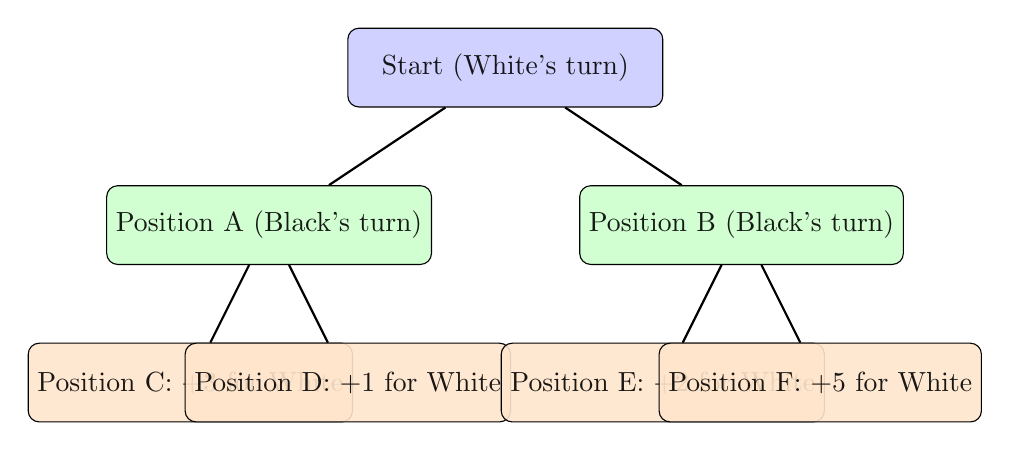
\begin{tikzpicture}[
        scale=1.0,
        transform shape,
        level distance=2cm,
        sibling distance=3cm,
        every node/.style={draw, rectangle, rounded corners, minimum width=4cm, minimum height=1cm, align=center, fill opacity=0.9}
    ]
        % Root node
        \node[fill=blue!20] (root) at (0,0) {Start (White's turn)};
        
        % Level 1 nodes
        \node[fill=green!20] (A) at (-3,-2) {Position A (Black's turn)};
        \node[fill=green!20] (B) at (3,-2) {Position B (Black's turn)};
        
        % Level 2 nodes
        \node[fill=orange!20] (C) at (-4,-4) {Position C: +3 for White};
        \node[fill=orange!20] (D) at (-2,-4) {Position D: +1 for White};
        \node[fill=orange!20] (E) at (2,-4) {Position E: +2 for White};
        \node[fill=orange!20] (F) at (4,-4) {Position F: +5 for White};
        
        % Connect nodes
        \draw[thick] (root) -- (A);
        \draw[thick] (root) -- (B);
        \draw[thick] (A) -- (C);
        \draw[thick] (A) -- (D);
        \draw[thick] (B) -- (E);
        \draw[thick] (B) -- (F);
    \end{tikzpicture}
    \caption{Minimax example with improved spacing and layout}
    \label{fig:minimax_example}
\end{figure}

\begin{figure}[ht]
    \centering
    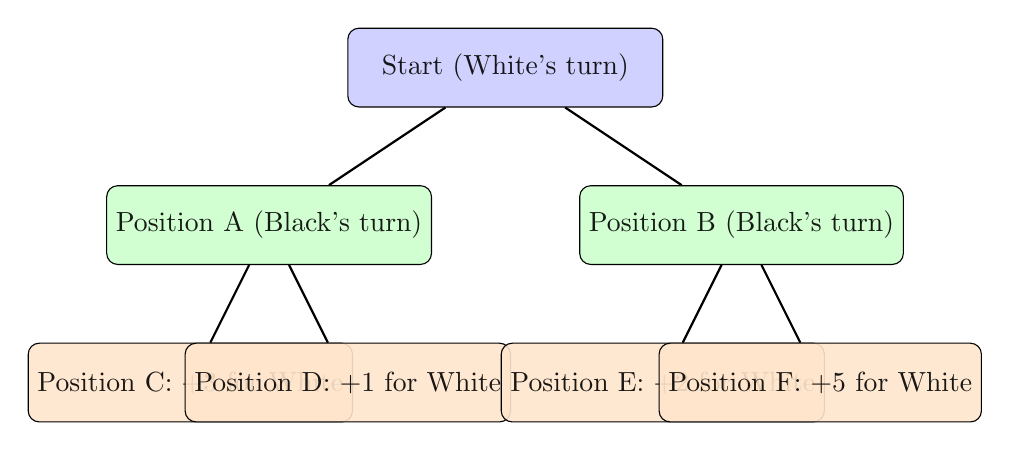
\begin{tikzpicture}[
        scale=1.0,
        transform shape,
        level distance=2cm,
        sibling distance=3cm,
        every node/.style={draw, rectangle, rounded corners, minimum width=4cm, minimum height=1cm, align=center, fill opacity=0.9}
    ]
        % Root node
        \node[fill=blue!20] (root) at (0,0) {Start (White's turn)};
        
        % Level 1 nodes
        \node[fill=green!20] (A) at (-3,-2) {Position A (Black's turn)};
        \node[fill=green!20] (B) at (3,-2) {Position B (Black's turn)};
        
        % Level 2 nodes
        \node[fill=orange!20] (C) at (-4,-4) {Position C: +3 for White};
        \node[fill=orange!20] (D) at (-2,-4) {Position D: +1 for White};
        \node[fill=orange!20] (E) at (2,-4) {Position E: +2 for White};
        \node[fill=orange!20] (F) at (4,-4) {Position F: +5 for White};
        
        % Connect nodes
        \draw[thick] (root) -- (A);
        \draw[thick] (root) -- (B);
        \draw[thick] (A) -- (C);
        \draw[thick] (A) -- (D);
        \draw[thick] (B) -- (E);
        \draw[thick] (B) -- (F);
    \end{tikzpicture}
    \caption{Minimax example with improved spacing and layout}
    \label{fig:minimax_example}
\end{figure}

\begin{figure}[ht]
    \centering
    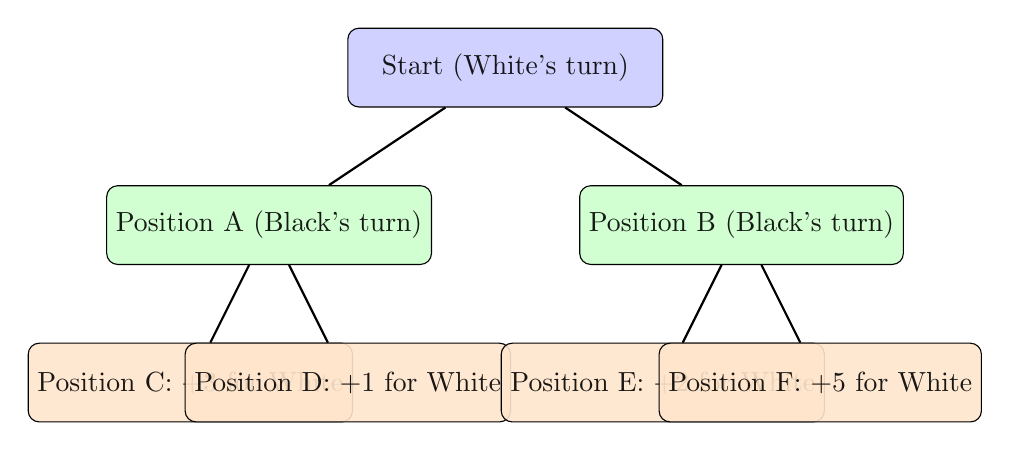
\begin{tikzpicture}[
        scale=1.0,
        transform shape,
        level distance=2cm,
        sibling distance=3cm,
        every node/.style={draw, rectangle, rounded corners, minimum width=4cm, minimum height=1cm, align=center, fill opacity=0.9}
    ]
        % Root node
        \node[fill=blue!20] (root) at (0,0) {Start (White's turn)};
        
        % Level 1 nodes
        \node[fill=green!20] (A) at (-3,-2) {Position A (Black's turn)};
        \node[fill=green!20] (B) at (3,-2) {Position B (Black's turn)};
        
        % Level 2 nodes
        \node[fill=orange!20] (C) at (-4,-4) {Position C: +3 for White};
        \node[fill=orange!20] (D) at (-2,-4) {Position D: +1 for White};
        \node[fill=orange!20] (E) at (2,-4) {Position E: +2 for White};
        \node[fill=orange!20] (F) at (4,-4) {Position F: +5 for White};
        
        % Connect nodes
        \draw[thick] (root) -- (A);
        \draw[thick] (root) -- (B);
        \draw[thick] (A) -- (C);
        \draw[thick] (A) -- (D);
        \draw[thick] (B) -- (E);
        \draw[thick] (B) -- (F);
    \end{tikzpicture}
    \caption{Minimax example with improved spacing and layout}
    \label{fig:minimax_example}
\end{figure}

\begin{figure}[ht]
    \centering
    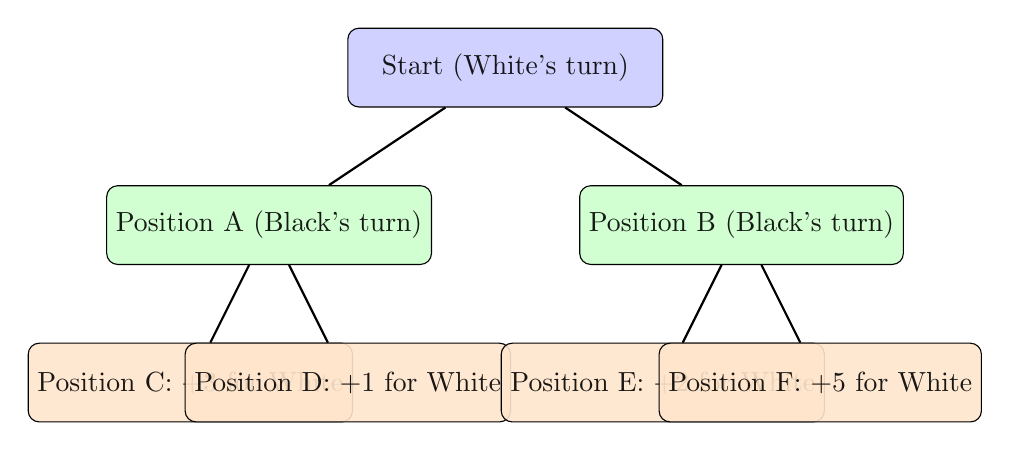
\begin{tikzpicture}[
        scale=1.0,
        transform shape,
        level distance=2cm,
        sibling distance=3cm,
        every node/.style={draw, rectangle, rounded corners, minimum width=4cm, minimum height=1cm, align=center, fill opacity=0.9}
    ]
        % Root node
        \node[fill=blue!20] (root) at (0,0) {Start (White's turn)};
        
        % Level 1 nodes
        \node[fill=green!20] (A) at (-3,-2) {Position A (Black's turn)};
        \node[fill=green!20] (B) at (3,-2) {Position B (Black's turn)};
        
        % Level 2 nodes
        \node[fill=orange!20] (C) at (-4,-4) {Position C: +3 for White};
        \node[fill=orange!20] (D) at (-2,-4) {Position D: +1 for White};
        \node[fill=orange!20] (E) at (2,-4) {Position E: +2 for White};
        \node[fill=orange!20] (F) at (4,-4) {Position F: +5 for White};
        
        % Connect nodes
        \draw[thick] (root) -- (A);
        \draw[thick] (root) -- (B);
        \draw[thick] (A) -- (C);
        \draw[thick] (A) -- (D);
        \draw[thick] (B) -- (E);
        \draw[thick] (B) -- (F);
    \end{tikzpicture}
    \caption{Minimax example with improved spacing and layout}
    \label{fig:minimax_example}
\end{figure}

\begin{figure}[ht]
    \centering
    \begin{tikzpicture}[
        scale=1.0,
        transform shape,
        level distance=2cm,
        sibling distance=3cm,
        every node/.style={draw, rectangle, rounded corners, minimum width=4cm, minimum height=1cm, align=center, fill opacity=0.9}
    ]
        % Root node
        \node[fill=blue!20] (root) at (0,0) {Start (White's turn)};
        
        % Level 1 nodes
        \node[fill=green!20] (A) at (-3,-2) {Position A (Black's turn)};
        \node[fill=green!20] (B) at (3,-2) {Position B (Black's turn)};
        
        % Level 2 nodes
        \node[fill=orange!20] (C) at (-4,-4) {Position C: +3 for White};
        \node[fill=orange!20] (D) at (-2,-4) {Position D: +1 for White};
        \node[fill=orange!20] (E) at (2,-4) {Position E: +2 for White};
        \node[fill=orange!20] (F) at (4,-4) {Position F: +5 for White};
        
        % Connect nodes
        \draw[thick] (root) -- (A);
        \draw[thick] (root) -- (B);
\documentclass[11pt, twocolumn]{article}
\setlength{\columnsep}{1.5cm}
\usepackage[left=1.5cm,right=1.5cm,top=2.5cm,bottom=2.5cm,columnsep=1.5cm]{geometry}

% Define a command for technical term explanations
\usepackage{amsthm}
\usepackage{tcolorbox}
\usepackage{xcolor}
\usepackage{amsmath}
\newtheorem{definition}{Definition}
\newenvironment{termbox}[1]
  {\begin{tcolorbox}[colback=blue!5!white,colframe=blue!75!black,title=#1,fonttitle=\bfseries]}
  {\end{tcolorbox}}
\usepackage{graphicx}
\usepackage{subcaption}
\usepackage{booktabs}
\usepackage{adjustbox}
\usepackage{tabularx}
\usepackage{multirow}
\usepackage{algorithm}
\usepackage{algpseudocode}
% Prevent redefinition of algorithmic commands
\providecommand{\algorithmicindent}{0em}
\usepackage{enumitem}
\usepackage{wrapfig}
\usepackage{cite}
\usepackage{amssymb,amsfonts}
\usepackage{textcomp}
\usepackage{listings}
\usepackage{hyperref}
\usepackage{float}
\usepackage{tikz}
\usetikzlibrary{shadows,arrows,shapes,positioning}
% Define fill opacity=0.9 style for TikZ
\tikzset{
  fill opacity=0.9/.style={
    general shadow={shadow xshift=0.7ex, shadow yshift=-0.7ex, opacity=0.4, fill=black!50, every shadow}
  }
}
\tikzset{every shadow/.style={}}
\usepackage{pgfplots}
\pgfplotsset{compat=1.18}
\usepackage{skak}
\usepackage{multicol}

% Define chess piece symbols with proper spacing
\newcommand{\WhitePawn}{\WhitePawnOnWhite\hspace{0.1em}}
\newcommand{\BlackPawn}{\BlackPawnOnWhite\hspace{0.1em}}
\newcommand{\WhiteRook}{\WhiteRookOnWhite\hspace{0.1em}}
\newcommand{\BlackRook}{\BlackRookOnWhite\hspace{0.1em}}
\newcommand{\WhiteKnight}{\WhiteKnightOnWhite\hspace{0.1em}}
\newcommand{\BlackKnight}{\BlackKnightOnWhite\hspace{0.1em}}
\newcommand{\WhiteBishop}{\WhiteBishopOnWhite\hspace{0.1em}}
\newcommand{\BlackBishop}{\BlackBishopOnWhite\hspace{0.1em}}
\newcommand{\WhiteQueen}{\WhiteQueenOnWhite\hspace{0.1em}}
\newcommand{\BlackQueen}{\BlackQueenOnWhite\hspace{0.1em}}
\newcommand{\WhiteKing}{\WhiteKingOnWhite\hspace{0.1em}}
\newcommand{\BlackKing}{\BlackKingOnWhite\hspace{0.1em}}

% Add the newunicodechar package to handle Unicode characters
\usepackage{newunicodechar}
\newunicodechar{♙}{\WhitePawn}
\newunicodechar{♟}{\BlackPawn}
\newunicodechar{♖}{\WhiteRook}
\newunicodechar{♜}{\BlackRook}
\newunicodechar{♘}{\WhiteKnight}
\newunicodechar{♞}{\BlackKnight}
\newunicodechar{♗}{\WhiteBishop}
\newunicodechar{♝}{\BlackBishop}
\newunicodechar{♕}{\WhiteQueen}
\newunicodechar{♛}{\BlackQueen}
\newunicodechar{♔}{\WhiteKing}
\newunicodechar{♚}{\BlackKing}
\newunicodechar{×}{$\times$}

% Define Unicode chess pieces with proper spacing
\DeclareUnicodeCharacter{2654}{\WhiteKing}
\DeclareUnicodeCharacter{2655}{\WhiteQueen}
\DeclareUnicodeCharacter{2656}{\WhiteRook}
\DeclareUnicodeCharacter{2657}{\WhiteBishop}
\DeclareUnicodeCharacter{2658}{\WhiteKnight}
\DeclareUnicodeCharacter{2659}{\WhitePawn}
\DeclareUnicodeCharacter{265A}{\BlackKing}
\DeclareUnicodeCharacter{265B}{\BlackQueen}
\DeclareUnicodeCharacter{265C}{\BlackRook}
\DeclareUnicodeCharacter{265D}{\BlackBishop}
\DeclareUnicodeCharacter{265E}{\BlackKnight}
\DeclareUnicodeCharacter{265F}{\BlackPawn}

% For multiplication symbol
\DeclareUnicodeCharacter{00D7}{$\times$}

% Fix algorithm package conflicts
\renewcommand{\algorithmicrequire}{\textbf{Input:}}
\renewcommand{\algorithmicensure}{\textbf{Output:}}

% Define colors for code listings
\definecolor{codegreen}{rgb}{0,0.6,0}
\definecolor{codegray}{rgb}{0.5,0.5,0.5}
\definecolor{codepurple}{rgb}{0.58,0,0.82}
\definecolor{backcolour}{rgb}{0.95,0.95,0.92}

% Configure code listings
\lstset{
    backgroundcolor=\color{backcolour},
    commentstyle=\color{codegreen},
    keywordstyle=\color{magenta},
    numberstyle=\tiny\color{codegray},
    stringstyle=\color{codepurple},
    basicstyle=\ttfamily\footnotesize,
    breakatwhitespace=false,
    breaklines=true,
    captionpos=b,
    keepspaces=true,
    numbers=left,
    numbersep=5pt,
    showspaces=false,
    showstringspaces=false,
    showtabs=false,
    tabsize=2
}

% Define Python style for listings
\lstdefinestyle{Python}{
    language=Python,
    morekeywords={self, if, else, return, try, except, raise, finally, import, from, as, def, class, for, while, with, True, False, None, and, or, not, in, is, lambda, yield, break, continue, pass, assert, del, global, nonlocal}
}

% Add spacing between sections
\usepackage{titlesec}
\titlespacing*{\section}{0pt}{3.5ex plus 1ex minus .2ex}{2.3ex plus .2ex}
\titlespacing*{\subsection}{0pt}{3.25ex plus 1ex minus .2ex}{1.5ex plus .2ex}

% Add spacing between items in lists
\setlist[itemize]{itemsep=0.2em, parsep=0.2em}
\setlist[enumerate]{itemsep=0.2em, parsep=0.2em}

% Add spacing between paragraphs
\setlength{\parskip}{0.5em}

% Add spacing between figures
\setlength{\floatsep}{1em}
\setlength{\textfloatsep}{1em}
\setlength{\intextsep}{1em}

\begin{document}

\title{Understanding Chess AI: From Simple Algorithms to Deep Reinforcement Learning\\\large A Beginner's Guide to Multi-Agent Deep Reinforcement Learning for Chess}
\author{Aditya Ranjan}
\date{}

\maketitle

\begin{abstract}
This document explains how computers play chess, starting from the simplest methods to advanced artificial intelligence. Written for beginners (even 10-year-olds can understand it!), we explore how chess-playing AI has evolved over time. We start with basic algorithms like Minimax, then move to more complex approaches like Monte Carlo Tree Search, and finally dive into modern deep reinforcement learning techniques. The document focuses on a specific project called Simple-MADRL-Chess, which uses multiple AI agents that learn by playing against each other. We explain every part of the code, how the neural networks work, and how the training process helps the AI get better at chess over time. Complete with examples, pictures, and step-by-step explanations, this guide makes complex AI concepts easy to understand.
\end{abstract}

\begin{center}
\textbf{Keywords:} Chess, Artificial Intelligence, Reinforcement Learning, Neural Networks, Minimax, Monte Carlo Tree Search, Multi-Agent Learning
\end{center}

\section{Introduction}
\subsection{What is Chess AI?}

Have you ever wondered how computers play chess? How do they know which moves to make? Can they really think like humans? In this document, we're going to explore the exciting world of chess-playing artificial intelligence (AI) in a way that anyone can understand - even if you're just 10 years old!

% --- Chessboard: Make it full-width and ensure rendering ---
\onecolumn

\begin{figure}[!htbp]
    \centering
    \newchessgame
    \setboardfontsize{28pt}
    \setchessboard{showmover=false, labelbottom=true, labelleft=true, boardfontfamily=lmss}
    \chessboard[setfen=rnbqkbnr/pppppppp/8/8/8/8/PPPPPPPP/RNBQKBNR]
    \caption{A chess board with pieces in starting position}
    \label{fig:chess_board}
\end{figure}

\twocolumn

Let's start with the basics of a chess board:
\begin{itemize}
    \item A chess board has 8 rows (called ranks) and 8 columns (called files)
    \item Each square is either light or dark
    \item There are 32 pieces total - 16 for each player
    \item Each type of piece moves differently
\end{itemize}

Chess AI is a computer program that can play chess by itself. It can analyze the board, think about possible moves, and choose what it believes is the best move. But computers don't "think" like we do. They follow instructions (called algorithms) that humans write for them. Over time, these algorithms have become more and more sophisticated, allowing computers to play chess at levels that can beat even the best human players in the world.

\subsection{Why Learn About Chess AI?}

Chess is a perfect game for teaching computers how to "think" because:
\begin{itemize}
    \item It has clear rules that don't change
    \item It requires planning and strategy
    \item You can measure how well you're doing (by winning or losing)
    \item It's complex enough to be interesting but simple enough to program
\end{itemize}

By understanding how chess AI works, you'll learn about many important concepts in computer science and artificial intelligence. These same ideas are used in self-driving cars, robots, game-playing systems, and many other exciting technologies!

\subsection{Our Journey Through Chess AI}

In this document, we'll take you on a journey through the evolution of chess AI:

\begin{enumerate}
    \item \textbf{Minimax Algorithm}

Let's start with the simplest way computers can play chess - the Minimax algorithm. Imagine you're playing a game of tic-tac-toe. You want to make the best move, but you also want to prevent your opponent from winning. That's exactly what Minimax does!

\begin{figure}[ht]
    \centering
    \begin{tikzpicture}[
        scale=1.0,
        transform shape,
        level distance=2cm,
        sibling distance=3cm,
        every node/.style={draw, rectangle, rounded corners, minimum width=4cm, minimum height=1cm, align=center, fill opacity=0.9}
    ]
        % Root node
        \node[fill=blue!20] (root) at (0,0) {Start (White's turn)};
        
        % Level 1 nodes
        \node[fill=green!20] (A) at (-3,-2) {Position A (Black's turn)};
        \node[fill=green!20] (B) at (3,-2) {Position B (Black's turn)};
        
        % Level 2 nodes
        \node[fill=orange!20] (C) at (-4,-4) {Position C: +3 for White};
        \node[fill=orange!20] (D) at (-2,-4) {Position D: +1 for White};
        \node[fill=orange!20] (E) at (2,-4) {Position E: +2 for White};
        \node[fill=orange!20] (F) at (4,-4) {Position F: +5 for White};
        
        % Connect nodes
        \draw[thick] (root) -- (A);
        \draw[thick] (root) -- (B);
        \draw[thick] (A) -- (C);
        \draw[thick] (A) -- (D);
        \draw[thick] (B) -- (E);
        \draw[thick] (B) -- (F);
    \end{tikzpicture}
    \caption{Minimax decision tree with improved spacing}
    \label{fig:minimax_tree}
\end{figure}

Here's how Minimax works:
\begin{enumerate}
    \item Look at all possible moves
    \item For each move, look at what your opponent could do
    \item For each of their moves, look at what you could do next
    \item Keep going until you reach the end of the game
    \item Choose the move that gives you the best outcome
\end{enumerate}, like Monte Carlo Tree Search.

    \item \textbf{Machine Learning}: Next, we'll see how computers can learn from experience instead of just following fixed rules.

    \item \textbf{Deep Reinforcement Learning}: Finally, we'll dive into modern AI techniques where computers teach themselves to play better by practicing millions of games.
\end{enumerate}

\subsection{The Simple-MADRL-Chess Project}

The main focus of this document is a special chess AI project called "Simple-MADRL-Chess." MADRL stands for "Multi-Agent Deep Reinforcement Learning." That's a fancy way of saying we have multiple AI players (agents) that learn by playing against each other and getting better over time.

We'll explain every part of this project in detail:
\begin{itemize}
    \item How the chess game is represented in the computer
    \item How the AI agents make decisions
    \item How they learn from their experiences
    \item How we train them to get better and better
\end{itemize}

By the end of this document, you'll understand how modern chess AI works, and you might even be inspired to create your own AI for chess or other games!

\section{The Basics of Chess AI}

\subsection{How Computers See Chess}

Before we dive into algorithms, let's understand how computers "see" a chess game. Unlike humans who look at the board and visually recognize pieces, computers need a way to represent the game mathematically.

\subsubsection{Board Representation}

The most common way to represent a chess board in a computer is using a grid of numbers, where each number represents a different piece. For example:
\begin{itemize}
    \item 0 might represent an empty square
    \item 1 might represent a white pawn
    \item 2 might represent a white knight
    \item And so on...
\end{itemize}

Here's a simple example of how a computer might see the starting position of a chess board:

\begin{center}
\begin{tabular}{|c|c|c|c|c|c|c|c|}
\hline
-3 & -2 & -3 & -5 & -6 & -3 & -2 & -3 \\
\hline
-1 & -1 & -1 & -1 & -1 & -1 & -1 & -1 \\
\hline
0 & 0 & 0 & 0 & 0 & 0 & 0 & 0 \\
\hline
0 & 0 & 0 & 0 & 0 & 0 & 0 & 0 \\
\hline
0 & 0 & 0 & 0 & 0 & 0 & 0 & 0 \\
\hline
0 & 0 & 0 & 0 & 0 & 0 & 0 & 0 \\
\hline
1 & 1 & 1 & 1 & 1 & 1 & 1 & 1 \\
\hline
3 & 2 & 3 & 5 & 6 & 3 & 2 & 3 \\
\hline
\end{tabular}
\end{center}

Where:
\begin{itemize}
    \item 1, -1 = White/Black Pawn
    \item 2, -2 = White/Black Knight
    \item 3, -3 = White/Black Bishop
    \item 5, -5 = White/Black Queen
    \item 6, -6 = White/Black King
\end{itemize}

In our Simple-MADRL-Chess project, we use a more sophisticated representation, but the basic idea is the same - convert the visual board into numbers that a computer can work with.

\subsubsection{Move Representation}

Computers also need a way to represent moves. A common approach is to use coordinates, where each square on the board has a unique address. For example, the move "e2 to e4" might be represented as (4,1) to (4,3) in a zero-indexed system.

\subsection{Evaluating Positions}

One of the most important parts of chess AI is the ability to evaluate a position. In other words, the computer needs to answer the question: "How good is this position for me?"

The simplest way to evaluate a position is to count the value of the pieces:
\begin{itemize}
    \item Pawn = 1 point
    \item Knight/Bishop = 3 points
    \item Rook = 5 points
    \item Queen = 9 points
    \item King = infinite points (since losing the king means losing the game)
\end{itemize}

So if White has all their pieces (worth 39 points) and Black is missing a knight (worth 3 points), then White has an advantage of 3 points.

More sophisticated evaluation functions also consider:
\begin{itemize}
    \item Piece positions (e.g., a knight in the center is better than a knight in the corner)
    \item King safety
    \item Pawn structure
    \item Control of the center
    \item Mobility (how many moves are available)
\end{itemize}

\subsection{The Minimax Algorithm}

Now that we understand how computers represent and evaluate chess positions, let's look at the simplest algorithm for playing chess: Minimax.

\subsubsection{How Minimax Works}

Minimax is based on a simple idea: assume both players will make the best possible moves. The algorithm works like this:

\begin{enumerate}
    \item Look at the current position
    \item Generate all possible moves
    \item For each move, evaluate what the board would look like after that move
    \item If it's your turn, choose the move that gives the highest evaluation
    \item If it's your opponent's turn, assume they will choose the move that gives the lowest evaluation (worst for you)
\end{enumerate}

The name "Minimax" comes from the fact that you're trying to maximize your minimum gain (or minimize your maximum loss).

\subsubsection{Minimax Example}

Let's see a simple example with a very small chess-like game:

\begin{center}
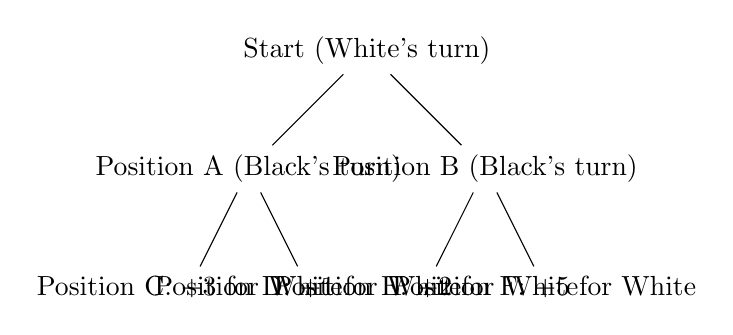
\begin{tikzpicture}[level distance=1.5cm,
  level 1/.style={sibling distance=3cm},
  level 2/.style={sibling distance=1.5cm}]
  \node {Start (White's turn)}
    child {node {Position A (Black's turn)}
      child {node {Position C: +3 for White}}
      child {node {Position D: +1 for White}}
    }
    child {node {Position B (Black's turn)}
      child {node {Position E: +2 for White}}
      child {node {Position F: +5 for White}}
    };
\end{tikzpicture}
\end{center}

In this example:
\begin{itemize}
    \item White has two possible moves from the start position, leading to positions A or B
    \item From position A, Black has two possible moves, leading to positions C or D
    \item From position B, Black has two possible moves, leading to positions E or F
    \item The numbers at the bottom are the evaluations (higher is better for White)
\end{itemize}

Using Minimax:
\begin{enumerate}
    \item If White chooses move A, Black will choose the move leading to position D (since +1 is worse for White than +3)
    \item If White chooses move B, Black will choose the move leading to position E (since +2 is worse for White than +5)
    \item So White's choices are effectively between positions D (+1) and E (+2)
    \item White will choose move B, leading to position E with a value of +2
\end{enumerate}

\subsubsection{Minimax with Depth}

The example above only looked one move ahead. In real chess, we want to look many moves ahead. We do this by applying Minimax recursively to a certain depth.

For example, if we set depth=4, the computer will look ahead 4 moves (2 moves by each player). The deeper we go, the better the computer will play, but the more calculations it needs to do.

\subsubsection{The Problem with Minimax}

The main problem with Minimax is that it grows exponentially with depth. In chess, each position has about 35 possible moves on average. So:
\begin{itemize}
    \item At depth 1: 35 positions to evaluate
    \item At depth 2: 35 × 35 = 1,225 positions
    \item At depth 3: 35 × 35 × 35 = 42,875 positions
    \item At depth 4: 35 × 35 × 35 × 35 = 1,500,625 positions
\end{itemize}

This quickly becomes too much for even the fastest computers. That's why we need more efficient algorithms, which we'll explore next.

\subsection{Alpha-Beta Pruning}

To make Minimax more efficient, we can use a technique called Alpha-Beta Pruning. This doesn't change the final decision, but it allows us to skip evaluating many positions that won't affect the outcome.

\subsubsection{How Alpha-Beta Pruning Works}

The key insight of Alpha-Beta Pruning is that once we find a good move, we can ignore moves that are clearly worse without fully evaluating them.

Let's go back to our example:

\begin{center}
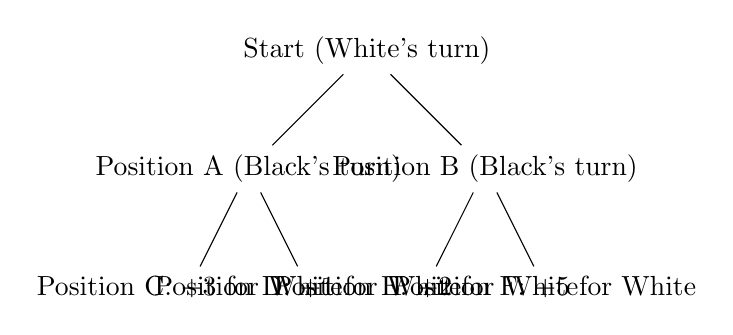
\begin{tikzpicture}[level distance=1.5cm,
  level 1/.style={sibling distance=3cm},
  level 2/.style={sibling distance=1.5cm}]
  \node {Start (White's turn)}
    child {node {Position A (Black's turn)}
      child {node {Position C: +3 for White}}
      child {node {Position D: +1 for White}}
    }
    child {node {Position B (Black's turn)}
      child {node {Position E: +2 for White}}
      child {node {Position F: +5 for White}}
    };
\end{tikzpicture}
\end{center}

With Alpha-Beta Pruning:
\begin{enumerate}
    \item White first explores move A
    \item Black's best response is move D, with value +1
    \item White then explores move B
    \item Black's first option is move E, with value +2
    \item Since +2 is already better than +1, White knows that move B is better than move A
    \item White doesn't need to explore Black's second option (move F) at all!
\end{enumerate}

In a real chess game with billions of possible positions, Alpha-Beta Pruning can eliminate huge portions of the search tree, allowing the computer to look much deeper in the same amount of time.

\subsubsection{Alpha-Beta Pruning in Code}

Here's a simplified version of how Alpha-Beta Pruning might be implemented in Python:

\begin{lstlisting}[style=Python]
def alpha_beta(position, depth, alpha, beta, maximizing_player):
    if depth == 0 or game_over(position):
        return evaluate(position)

    if maximizing_player:
        max_eval = float('-inf')
        for move in get_possible_moves(position):
            new_position = make_move(position, move)
            eval = alpha_beta(new_position, depth-1, alpha, beta, False)
            max_eval = max(max_eval, eval)
            alpha = max(alpha, eval)
            if beta <= alpha:
                break  # Beta cutoff
        return max_eval
    else:
        min_eval = float('inf')
        for move in get_possible_moves(position):
            new_position = make_move(position, move)
            eval = alpha_beta(new_position, depth-1, alpha, beta, True)
            min_eval = min(min_eval, eval)
            beta = min(beta, eval)
            if beta <= alpha:
                break  # Alpha cutoff
        return min_eval
\end{lstlisting}

The key part is the `if beta <= alpha: break` line, which is where we "prune" branches that won't affect the final decision.

\subsection{Monte Carlo Tree Search}

While Minimax with Alpha-Beta Pruning was the dominant approach in chess AI for decades, a newer algorithm called Monte Carlo Tree Search (MCTS) has become popular in recent years, especially for games like Go.

\subsubsection{How MCTS Works}

MCTS is based on random sampling. Instead of trying to evaluate every possible move, it plays many random games (simulations) from the current position and keeps track of which moves tend to lead to wins.

The algorithm has four main steps:
\begin{enumerate}
    \item \textbf{Selection}: Start from the root (current position) and select successive child nodes until reaching a leaf node. The selection is based on a formula that balances exploration (trying new moves) and exploitation (focusing on promising moves).

    \item \textbf{Expansion}: If the leaf node is not a terminal state (end of game), create one or more child nodes and select one.

    \item \textbf{Simulation}: Play a random game from the selected node until reaching a terminal state.

    \item \textbf{Backpropagation}: Update the statistics of all nodes in the path from the selected node to the root based on the result of the simulation.
\end{enumerate}

\subsubsection{MCTS Example}

Let's see a simple example of how MCTS might work in a chess-like game:

\begin{enumerate}
    \item We start at the current position and have three possible moves: A, B, and C.

    \item We haven't tried any of them yet, so we select move A (randomly).

    \item From position A, we play a random game until someone wins. Let's say White wins.

    \item We update the statistics for move A: 1 win out of 1 game.

    \item Next iteration, we select move B (to explore all options).

    \item From position B, we play a random game. Let's say Black wins.

    \item We update the statistics for move B: 0 wins out of 1 game.

    \item Next iteration, we select move C.

    \item From position C, we play a random game. Let's say White wins.

    \item We update the statistics for move C: 1 win out of 1 game.

    \item Now all moves have been tried once. In future iterations, we'll select based on which moves have the highest win rate, but also occasionally try moves with lower win rates (to make sure we don't miss anything).
\end{enumerate}

After many iterations (thousands or millions), we'll have a good estimate of which move is best.

\subsubsection{MCTS vs. Minimax}

MCTS has several advantages over Minimax:
\begin{itemize}
    \item It doesn't need an evaluation function (it just needs to know who won the game)
    \item It can be stopped at any time and will still give a reasonable move
    \item It naturally focuses on the most promising variations
    \item It handles uncertainty and randomness well
\end{itemize}

However, MCTS also has disadvantages:
\begin{itemize}
    \item It can miss tactical opportunities that Minimax would find
    \item It requires many simulations to be effective
    \item In games with a high branching factor (like chess), the random simulations might not be very informative
\end{itemize}

\subsubsection{MCTS in Code}

Here's a simplified version of how MCTS might be implemented in Python:

\begin{lstlisting}[style=Python]
import math
import random

class Node:
    def __init__(self, state, parent=None, move=None):
        self.state = state
        self.parent = parent
        self.move = move
        self.children = []
        self.wins = 0
        self.visits = 0
        self.untried_moves = get_possible_moves(state)

    def select_child(self):
        # UCB1 formula for selection
        s = sorted(self.children, key=lambda c: c.wins/c.visits +
                  math.sqrt(2*math.log(self.visits)/c.visits))
        return s[-1]  # Return the child with the highest UCB1 value

    def expand(self):
        move = self.untried_moves.pop()
        new_state = make_move(self.state, move)
        child = Node(new_state, self, move)
        self.children.append(child)
        return child

    def update(self, result):
        self.visits += 1
        self.wins += result

def monte_carlo_tree_search(root_state, iterations):
    root = Node(root_state)

    for _ in range(iterations):
        # Selection
        node = root
        while node.untried_moves == [] and node.children != []:
            node = node.select_child()

        # Expansion
        if node.untried_moves != []:
            node = node.expand()

        # Simulation
        state = node.state
        while not game_over(state):
            moves = get_possible_moves(state)
            move = random.choice(moves)
            state = make_move(state, move)

        # Backpropagation
        result = 1 if white_wins(state) else 0
        while node is not None:
            node.update(result)
            node = node.parent

    # Return the move with the highest number of visits
    return sorted(root.children, key=lambda c: c.visits)[-1].move
\end{lstlisting}

This is a basic implementation of MCTS. In practice, there are many optimizations and variations of this algorithm.

\section{Machine Learning for Chess}

So far, we've looked at traditional algorithms where humans explicitly program the rules for how the computer should play chess. Now, let's explore how computers can learn to play chess on their own through machine learning.

\subsection{From Handcrafted Rules to Learning}

Traditional chess engines like Stockfish use handcrafted evaluation functions created by chess experts. These functions consider factors like piece values, king safety, pawn structure, etc. While effective, creating and tuning these functions requires a lot of human expertise.

Machine learning takes a different approach: instead of telling the computer exactly how to evaluate positions, we let it learn from data. This has several advantages:
\begin{itemize}
    \item The computer might discover patterns that humans haven't noticed
    \item The evaluation can be more nuanced and adapt to different styles of play
    \item We don't need chess experts to create the evaluation function
\end{itemize}

\subsection{Neural Networks}

The most common type of machine learning model used in modern chess AI is the neural network. Neural networks are loosely inspired by how the human brain works, with interconnected "neurons" that process information.

\subsubsection{How Neural Networks Work}

A neural network consists of layers of neurons:
\begin{itemize}
    \item \textbf{Input Layer}: Receives the initial data (in chess, this would be the board position)
    \item \textbf{Hidden Layers}: Process the information through a series of mathematical operations
    \item \textbf{Output Layer}: Produces the final result (in chess, this might be an evaluation of the position or a probability distribution over possible moves)
\end{itemize}

Each neuron takes inputs from the previous layer, applies weights to them, sums them up, and then applies an "activation function" to produce its output. The weights are what the network learns during training.

\subsubsection{Neural Network Example}

Here's a simple example of how a neural network might evaluate a chess position:

\begin{enumerate}
    \item \textbf{Input}: The board position, represented as a 64-element array (one for each square), where each element indicates what piece (if any) is on that square.

    \item \textbf{Hidden Layer 1}: Might learn to recognize patterns like "knight fork" or "queen in danger."

    \item \textbf{Hidden Layer 2}: Might combine these patterns to understand concepts like "attacking position" or "defensive structure."

    \item \textbf{Output}: A single number representing the evaluation of the position (positive for White advantage, negative for Black advantage).
\end{enumerate}

\subsubsection{Training Neural Networks}

Neural networks learn by adjusting their weights based on examples. For chess, we might train a network by:
\begin{itemize}
    \item Showing it millions of positions from real games
    \item For each position, telling it who eventually won the game
    \item Adjusting the weights so that the network's evaluation better predicts the winner
\end{itemize}

This process is called "supervised learning" because we're supervising the network by providing the correct answers.

\subsection{Reinforcement Learning}

While supervised learning is powerful, it requires a large dataset of labeled examples. Reinforcement learning (RL) is another approach where the computer learns by playing against itself and receiving rewards for good moves.

\subsubsection{How Reinforcement Learning Works}

In reinforcement learning:
\begin{enumerate}
    \item The agent (our chess AI) observes the current state (the board position)
    \item It takes an action (makes a move)
    \item It receives a reward (e.g., +1 for winning, -1 for losing, 0 for drawing)
    \item It updates its policy (strategy for choosing moves) to maximize future rewards
\end{enumerate}

The key insight is that the agent doesn't need to be told exactly what to do in each situation. It learns through trial and error, gradually improving its policy.

\subsubsection{Policy and Value Functions}

In reinforcement learning for chess, we typically have two main components:
\begin{itemize}
    \item \textbf{Policy Function}: Decides which move to make in a given position
    \item \textbf{Value Function}: Estimates how good a position is
\end{itemize}

Both of these can be represented by neural networks:
\begin{itemize}
    \item The policy network takes a board position as input and outputs a probability distribution over possible moves
    \item The value network takes a board position as input and outputs an estimate of who will win from that position
\end{itemize}

\subsubsection{Self-Play}

One of the most effective ways to train a reinforcement learning agent for chess is through self-play:
\begin{enumerate}
    \item Start with a randomly initialized policy
    \item Have the agent play games against itself
    \item Use the outcomes of these games to improve the policy
    \item Repeat with the improved policy
\end{enumerate}

This approach was used by AlphaZero, a chess AI developed by DeepMind that famously defeated Stockfish (one of the strongest traditional chess engines) after learning to play chess in just 24 hours of self-play.

\section{Deep Reinforcement Learning}
\subsection{PPO Algorithm: From Basics to Advanced}

\subsubsection{Understanding Reinforcement Learning Basics}

Before diving into PPO, let's understand the basic reinforcement learning concepts. Imagine you're teaching a child to play chess:

\begin{enumerate}
    \item The child looks at the chess board (this is the \textbf{state} $s$)
    \item The child makes a move (this is the \textbf{action} $a$)
    \item You tell them if the move was good or bad (this is the \textbf{reward} $r$)
    \item The board changes to a new position (this is the \textbf{next state} $s'$)
    \item This process repeats until the game ends
\end{enumerate}

In mathematical terms, at each timestep $t$, the agent:
\begin{itemize}
    \item Observes state $s_t$
    \item Takes action $a_t$
    \item Receives reward $r_t$
    \item Transitions to state $s_{t+1}$
\end{itemize}

The goal is to find a policy $\pi(a|s)$ that maximizes the expected cumulative reward:

\begin{equation}
    J(\pi) = \mathbb{E}_{\tau \sim \pi} \left[ \sum_{t=0}^{T} \gamma^t r_t \right]
\end{equation}

Where:
\begin{itemize}
    \item $\pi(a|s)$ is our policy - it tells us the probability of taking action $a$ in state $s$
    \item $\tau$ is a trajectory (a complete sequence of states, actions, and rewards)
    \item $\gamma$ is a discount factor (value between 0 and 1) that makes future rewards worth less than immediate rewards
    \item $r_t$ is the reward at time step $t$
    \item $T$ is the time horizon (length of the game)
    \item $\mathbb{E}_{\tau \sim \pi}$ means the expected value over all possible trajectories when following policy $\pi$
\end{itemize}

\subsubsection*{Example with Chess}
Imagine a simple chess scenario:
\begin{itemize}
    \item You capture an opponent's pawn (+1 reward)
    \item Two moves later, you capture a knight (+3 reward)
    \item Three moves after that, you capture the queen (+9 reward)
    \item Finally, after two more moves, you checkmate (+50 reward)
\end{itemize}

With a discount factor $\gamma = 0.9$, your cumulative discounted reward would be:
\begin{align*}
    J &= 1 + 0.9^2 \times 3 + 0.9^5 \times 9 + 0.9^7 \times 50 \\
    &= 1 + 0.81 \times 3 + 0.59049 \times 9 + 0.47829 \times 50 \\
    &= 1 + 2.43 + 5.31 + 23.91 \\
    &= 32.65
\end{align*}

If we didn't use discounting ($\gamma = 1$), the sum would simply be $1 + 3 + 9 + 50 = 63$. The discounting makes immediate rewards more valuable than delayed rewards, encouraging the agent to achieve goals sooner rather than later.

\subsubsection{Value Functions and Advantages}

We use two important functions in reinforcement learning:
\begin{itemize}
    \item \textbf{Value function} $V^\pi(s)$: How good is it to be in state $s$? This estimates the total expected future reward from being in state $s$ and following policy $\pi$ afterward.
    \item \textbf{Q-function} $Q^\pi(s,a)$: How good is it to take action $a$ in state $s$? This estimates the total expected future reward from taking action $a$ in state $s$ and then following policy $\pi$ afterward.
\end{itemize}

Mathematically:
\begin{equation}
    V^\pi(s) = \mathbb{E}_{\tau \sim \pi} \left[ \sum_{t=0}^{T} \gamma^t r_t | s_0 = s \right]
\end{equation}

This equation means: "What's the expected total reward if I start in state $s$ and follow policy $\pi$ all the way to the end of the game?"

\begin{equation}
    Q^\pi(s,a) = \mathbb{E}_{\tau \sim \pi} \left[ \sum_{t=0}^{T} \gamma^t r_t | s_0 = s, a_0 = a \right]
\end{equation}

This equation means: "What's the expected total reward if I take action $a$ in state $s$ right now, and then follow policy $\pi$ all the way to the end of the game?"

\subsubsection*{Chess Example for Value Function}
Imagine you're evaluating a chess position:
\begin{itemize}
    \item Position A: You have a queen advantage, and your opponent's king is exposed. Value function might estimate: $V(\text{Position A}) = +8$ (very good for you)
    \item Position B: Equal material, but your pieces are poorly positioned. Value function might estimate: $V(\text{Position B}) = -1$ (slightly bad for you)
\end{itemize}

\subsubsection*{Chess Example for Q-Function}
For a given position, different moves have different Q-values:
\begin{itemize}
    \item Move 1: Capture opponent's queen with your knight. $Q(\text{Position}, \text{Capture Queen}) = +7$ (excellent move)
    \item Move 2: Move your pawn forward one square. $Q(\text{Position}, \text{Advance Pawn}) = +0.5$ (slightly good move)
    \item Move 3: Move your king into check. $Q(\text{Position}, \text{King into Check}) = -10$ (terrible move)
\end{itemize}

The \textbf{advantage function} tells us how much better an action is compared to the average action:
\begin{equation}
    A^\pi(s,a) = Q^\pi(s,a) - V^\pi(s)
\end{equation}

This is extremely important because it tells us which actions are better than the average action in a given state. It's the key to learning which actions to prefer.

\subsubsection*{Chess Example for Advantage Function}
Imagine a position where the overall value is $V(\text{Position}) = +2$ (slightly good for you). For different moves:
\begin{itemize}
    \item Move 1: Capture opponent's queen. $Q(\text{Position}, \text{Capture Queen}) = +9$
    $\Rightarrow$ Advantage = $Q(\text{Position}, \text{Capture Queen}) - V(\text{Position}) = +9 - (+2) = +7$ (much better than average)
    
    \item Move 2: Move pawn forward. $Q(\text{Position}, \text{Advance Pawn}) = +2$
    $\Rightarrow$ Advantage = $Q(\text{Position}, \text{Advance Pawn}) - V(\text{Position}) = +2 - (+2) = 0$ (exactly average)
    
    \item Move 3: Blunder your bishop. $Q(\text{Position}, \text{Blunder Bishop}) = -3$
    $\Rightarrow$ Advantage = $Q(\text{Position}, \text{Blunder Bishop}) - V(\text{Position}) = -3 - (+2) = -5$ (much worse than average)
\end{itemize}

The agent will learn to prefer actions with positive advantage and avoid actions with negative advantage.

\subsubsection{From Basic RL to PPO}

Proximal Policy Optimization (PPO) is an advanced reinforcement learning algorithm that makes learning more stable and efficient. Imagine PPO as a smart robot learning to play chess. Let's break it down into simple parts:

\begin{figure}[h]
    \centering
    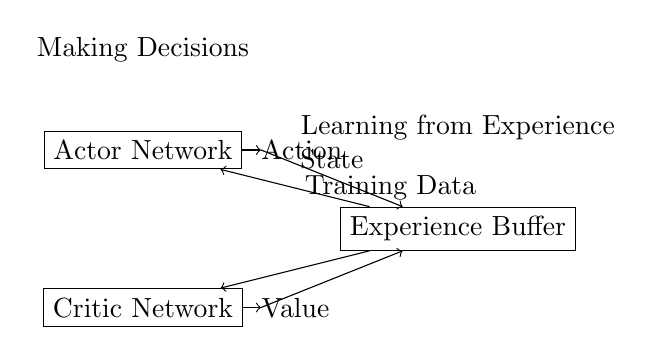
\begin{tikzpicture}
        \node[draw, rectangle] (actor) at (0,2) {Actor Network};
        \node[draw, rectangle] (critic) at (0,0) {Critic Network};
        \node[draw, rectangle] (buffer) at (4,1) {Experience Buffer};
        
        \draw[->] (actor) -- node[right] {Action} (1.5,2);
        \draw[->] (critic) -- node[right] {Value} (1.5,0);
        \draw[->] (1.5,2) -- node[above] {State} (buffer);
        \draw[->] (1.5,0) -- (buffer);
        \draw[->] (buffer) -- node[right] {Training Data} (actor);
        \draw[->] (buffer) -- (critic);
        
        \node[above] at (0,3) {Making Decisions};
        \node[above] at (4,2) {Learning from Experience};
    \end{tikzpicture}
    \caption{PPO Architecture}
    \label{fig:ppo_architecture}
\end{figure}

\subsubsection{The Actor Network}
Think of the Actor as a smart chess player who decides which moves to make. It looks at the chess board (state) and chooses the best move based on what it has learned.

\subsubsection{The Critic Network}
The Critic is like a coach who tells the Actor if its moves were good or bad. It gives feedback about how well the move might work.

\subsubsection{Experience Buffer}
The Buffer is like a notebook where the robot writes down all its experiences. It remembers:
\begin{itemize}
    \item What moves it made (actions)
    \item How good those moves were (values)
    \item What happened after each move (rewards)
\end{itemize}

\subsection{How PPO Learns}

PPO learns through a process called "self-play." Here's how it works:

\begin{enumerate}
    \item The robot plays many games against itself
    \item It records every move and what happened
    \item The Critic evaluates how good each move was
    \item The Actor learns from this feedback
    \item The process repeats, getting better each time
\end{enumerate}

\begin{figure}[h]
    \centering
    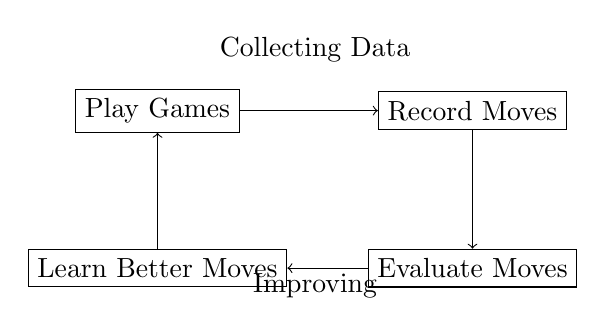
\begin{tikzpicture}
        \node[draw, rectangle] (play) at (0,2) {Play Games};
        \node[draw, rectangle] (record) at (4,2) {Record Moves};
        \node[draw, rectangle] (evaluate) at (4,0) {Evaluate Moves};
        \node[draw, rectangle] (learn) at (0,0) {Learn Better Moves};
        
        \draw[->] (play) -- (record);
        \draw[->] (record) -- (evaluate);
        \draw[->] (evaluate) -- (learn);
        \draw[->] (learn) -- (play);
        
        \node[above] at (2,2.5) {Collecting Data};
        \node[above] at (2,-0.5) {Improving};
    \end{tikzpicture}
    \caption{PPO Learning Process}
    \label{fig:ppo_learning}
\end{figure}

\subsection{Key Components}

\subsubsection{Buffer}
The Buffer stores all the robot's experiences. It's like a big memory box that helps the robot remember:
\begin{itemize}
    \item States: Different chess board positions
    \item Actions: Moves that were made
    \item Rewards: How good the moves were
    \item Advantages: How much better a move was than average
\end{itemize}

\subsubsection{Learning Process}

The learning process has several important steps:
\begin{enumerate}
    \item \textbf{Action Selection}: The robot decides what move to make
    \item \textbf{Value Estimation}: It guesses how good the move might be
    \item \textbf{Experience Collection}: It records what happens
    \item \textbf{Training}: It learns from its experiences
\end{enumerate}

\subsection{The PPO Algorithm in Detail}

\subsubsection{The PPO Objective Function}

PPO introduces a clever way to update the policy without making too large changes. The key innovation is the PPO objective function:

\begin{equation}
    L^{CLIP}(\theta) = \mathbb{E}_t \left[ \min(r_t(\theta) A_t, \text{clip}(r_t(\theta), 1-\epsilon, 1+\epsilon) A_t) \right]
\end{equation}

Where:
\begin{itemize}
    \item $r_t(\theta) = \frac{\pi_\theta(a_t|s_t)}{\pi_{\theta_{old}}(a_t|s_t)}$ is the probability ratio between the new and old policies
    \item $A_t$ is the advantage estimate for action $a_t$ in state $s_t$
    \item $\epsilon$ is a hyperparameter (typically 0.1 or 0.2) that limits how much the policy can change in a single update
    \item $\text{clip}(r_t(\theta), 1-\epsilon, 1+\epsilon)$ clips the ratio to be between $[1-\epsilon, 1+\epsilon]$
\end{itemize}

\subsubsection*{Breaking Down the PPO Formula}

To really understand PPO, let's break it down step-by-step:

1. \textbf{Probability Ratio}: $r_t(\theta) = \frac{\pi_\theta(a_t|s_t)}{\pi_{\theta_{old}}(a_t|s_t)}$ compares how likely an action is under the new policy versus the old policy.
   - If $r_t = 1$: The new policy thinks this action is just as good as the old policy did
   - If $r_t = 1.5$: The new policy thinks this action is 50\% better than the old policy did
   - If $r_t = 0.7$: The new policy thinks this action is 30\% worse than the old policy did

2. \textbf{The Clipping Mechanism}: $\text{clip}(r_t(\theta), 1-\epsilon, 1+\epsilon)$ prevents the ratio from being too far from 1.
   - If $\epsilon = 0.2$ and $r_t = 1.3$, the clipped value is still 1.2 (within bounds)
   - If $\epsilon = 0.2$ and $r_t = 1.5$, the clipped value becomes 1.2 (clipped down)
   - If $\epsilon = 0.2$ and $r_t = 0.7$, the clipped value is still 0.7 (within bounds)
   - If $\epsilon = 0.2$ and $r_t = 0.6$, the clipped value becomes 0.8 (clipped up)

3. \textbf{The Min Operation}: $\min(r_t(\theta) A_t, \text{clip}(r_t(\theta), 1-\epsilon, 1+\epsilon) A_t)$ makes training even more conservative.

\subsubsection*{Chess Example of PPO in Action}

Let's see how PPO works with a chess example:

Suppose our chess agent considers a move "Capture opponent's knight with bishop":

\begin{itemize}
    \item The old policy: $\pi_{\theta_{old}}(\text{capture knight}|\text{current board}) = 0.2$ (20\% probability)
    \item The new policy: $\pi_{\theta}(\text{capture knight}|\text{current board}) = 0.4$ (40\% probability)
    \item The ratio: $r_t = \frac{0.4}{0.2} = 2.0$ (the new policy thinks this move is twice as good)
    \item The advantage: $A_t = +3$ (this is actually a good move)
    \item With $\epsilon = 0.2$, the clipped ratio is $\min(2.0, 1.2) = 1.2$
\end{itemize}

So our PPO update will be:
\begin{align*}
    \min(r_t A_t, \text{clip}(r_t) A_t) &= \min(2.0 \times 3, 1.2 \times 3) \\
    &= \min(6.0, 3.6) \\
    &= 3.6
\end{align*}

Instead of updating with a factor of $6.0$ (which could be unstable), we update with $3.6$, making the learning more stable.

Now consider a different move "Move pawn forward unnecessarily":

\begin{itemize}
    \item Advantage: $A_t = -2$ (this is a bad move)
    \item Old policy probability: $\pi_{\theta_{old}}(\text{move pawn}|\text{board}) = 0.1$
    \item New policy probability: $\pi_{\theta}(\text{move pawn}|\text{board}) = 0.05$
    \item Ratio: $r_t = \frac{0.05}{0.1} = 0.5$
    \item With $\epsilon = 0.2$, the clipped ratio is $\max(0.5, 0.8) = 0.8$
\end{itemize}

Our PPO update would be:
\begin{align*}
    \min(r_t A_t, \text{clip}(r_t) A_t) &= \min(0.5 \times (-2), 0.8 \times (-2)) \\
    &= \min(-1.0, -1.6) \\
    &= -1.0
\end{align*}

Here, we use the unclipped value because it gives a less negative result (remember we're trying to maximize our objective).

This clipping mechanism is why PPO is so effective - it prevents wild swings in the policy during training, leading to more stable and reliable learning.

\subsubsection{Generalized Advantage Estimation (GAE)}

Calculating advantages accurately is crucial for PPO to work well. PPO uses a technique called Generalized Advantage Estimation (GAE) to calculate better advantage estimates:

\begin{equation}
    A^{GAE(\gamma, \lambda)}_t = \sum_{l=0}^{\infty} (\gamma \lambda)^l \delta_{t+l}
\end{equation}

Where $\delta_t = r_t + \gamma V(s_{t+1}) - V(s_t)$ is the temporal difference (TD) error.

\subsubsection*{Understanding TD Error}

The temporal difference error $\delta_t$ can be understood as "how surprised we were by the reward". It compares:
\begin{itemize}
    \item What we actually got: $r_t + \gamma V(s_{t+1})$ (immediate reward plus discounted value of next state)
    \item What we expected: $V(s_t)$ (our estimate of the current state's value)
\end{itemize}

If $\delta_t > 0$, the action was better than expected. If $\delta_t < 0$, the action was worse than expected.

\subsubsection*{The GAE Formula Explained}

GAE computes advantage by looking at a weighted sum of all future TD errors:
\begin{itemize}
    \item $\delta_t$ gets full weight
    \item $\delta_{t+1}$ gets weight $(\gamma \lambda)$
    \item $\delta_{t+2}$ gets weight $(\gamma \lambda)^2$
    \item And so on...
\end{itemize}

In practice, we compute this recursively, starting from the end of an episode and working backward:
\begin{equation}
    A_t = \delta_t + \gamma \lambda A_{t+1}
\end{equation}

\subsubsection*{Chess Example of GAE}

Let's see how GAE works with a chess example. Imagine we're tracking a 3-move sequence with $\gamma = 0.9$ and $\lambda = 0.95$:

\begin{itemize}
    \item Move 1: Advance pawn
        \begin{itemize}
            \item Reward $r_1 = 0$ (no immediate benefit)
            \item Current state value $V(s_1) = 2$ (slightly good position)
            \item Next state value $V(s_2) = 3$ (better position after pawn move)
            \item TD error: $\delta_1 = 0 + 0.9 \times 3 - 2 = 0.7$ (slightly better than expected)
        \end{itemize}
    
    \item Move 2: Capture opponent's knight
        \begin{itemize}
            \item Reward $r_2 = 3$ (captured a knight worth 3 points)
            \item Current state value $V(s_2) = 3$
            \item Next state value $V(s_3) = 5$ (even better position)
            \item TD error: $\delta_2 = 3 + 0.9 \times 5 - 3 = 4.5$ (much better than expected)
        \end{itemize}
    
    \item Move 3: Set up checkmate
        \begin{itemize}
            \item Reward $r_3 = 0$ (no immediate capture)
            \item Current state value $V(s_3) = 5$
            \item Next state value $V(s_4) = 9$ (winning position)
            \item TD error: $\delta_3 = 0 + 0.9 \times 9 - 5 = 3.1$ (better than expected)
        \end{itemize}
\end{itemize}

Now we calculate the advantages backwards:
\begin{align*}
    A_3 &= \delta_3 = 3.1 \\
    A_2 &= \delta_2 + \gamma \lambda A_3 = 4.5 + 0.9 \times 0.95 \times 3.1 \approx 7.14 \\
    A_1 &= \delta_1 + \gamma \lambda A_2 = 0.7 + 0.9 \times 0.95 \times 7.14 \approx 6.84
\end{align*}

Notice how the advantage of the first move ($A_1 = 6.84$) is very high, even though its immediate TD error was small ($\delta_1 = 0.7$). This is because GAE correctly assigns credit to the first move for setting up the subsequent good moves.

\section{Chess Environment Representation}

\subsection{How Chess is Represented for the AI}

Before we can teach an AI to play chess, we need to represent the chess board in a way the computer can understand. Let's explore how the chess environment is implemented.

\subsubsection{Board Representation}

The chess board is represented as a multi-dimensional array. Each position on the board contains information about:

\begin{itemize}
    \item What piece is on that square (pawn, knight, bishop, rook, queen, king, or empty)
    \item Which player owns that piece (white or black)
    \item Special states like whether a king has castling rights or if a pawn can be captured en passant
\end{itemize}

\begin{figure}[h]
    \centering
    \begin{tikzpicture}[scale=1.2]
        % Define colors
        \colorlet{light}{white}
        \colorlet{dark}{black!60}
        
        % Draw the checkered board
        \foreach \i in {0,...,7} {
            \foreach \j in {0,...,7} {
                \pgfmathsetmacro{\colorfill}{mod(\i+\j,2) ? "light" : "dark"}
                \fill[\colorfill] (\i*0.6,\j*0.6) rectangle +(0.6,0.6);
                \node[font=\tiny] at (\i*0.6+0.1, \j*0.6+0.1) {$c_{\i,\j}$};
            }
        }
        
        % Add file labels (a-h) at the bottom
        \foreach \i [count=\xi from 0] in {a,...,h}
            \node at (\xi*0.6+0.3, -0.2) {\i};
            
        % Add rank labels (1-8) on the left
        \foreach \i [count=\xi from 0] in {1,...,8}
            \node at (-0.2, \xi*0.6-0.3) {\i};
        
        % Add some sample pieces
        \node at (0*0.6+0.3, 0*0.6+0.3) {\LARGE ♜}; % Black rook
        \node at (1*0.6+0.3, 0*0.6+0.3) {\LARGE ♞}; % Black knight
        \node at (0*0.6+0.3, 1*0.6+0.3) {\LARGE ♟}; % Black pawn
        
        \node at (6*0.6+0.3, 6*0.6+0.3) {\LARGE ♙}; % White pawn
        \node at (7*0.6+0.3, 7*0.6+0.3) {\LARGE ♖}; % White rook
        \node at (6*0.6+0.3, 7*0.6+0.3) {\LARGE ♘}; % White knight
        \node at (4*0.6+0.3, 7*0.6+0.3) {\LARGE ♔}; % White king
        \node at (3*0.6+0.3, 7*0.6+0.3) {\LARGE ♕}; % White queen
    \end{tikzpicture}
    \caption{A chess board with pieces and coordinates $c_{x,y}$}
    \label{fig:chess_array}
\end{figure}

\subsubsection{State Encoding}

To feed the board state into our neural networks, we encode it as a multi-channel 2D array. Each channel represents different information:

\begin{itemize}
    \item Channel 1-6: White pieces (pawn, knight, bishop, rook, queen, king)
    \item Channel 7-12: Black pieces (pawn, knight, bishop, rook, queen, king)
    \item Additional channels for special information (whose turn it is, castling rights, etc.)
\end{itemize}

Here's a simplified example of how we represent a white pawn at position (2,1):

\begin{lstlisting}[style=Python]
# Channel 1 (White Pawns)
board[0, 2, 1] = 1  # Set to 1 for white pawn at position (2,1)
\end{lstlisting}

\subsubsection{Move Encoding}

Chess moves are encoded as integers from 0 to 4095, representing all possible combinations of:
\begin{itemize}
    \item Starting square (64 possibilities)
    \item Ending square (64 possibilities)
    \item Special move types (promotion to knight, bishop, rook, or queen)
\end{itemize}

In our implementation, we map this to an action space of 0-4095, but we also use a move mask to ensure only legal moves are selected.

\begin{lstlisting}[style=Python]
def encode_move(from_square, to_square, promotion=None):
    # Convert chess squares to 0-63 indices
    from_idx = from_square.index
    to_idx = to_square.index
    
    # Base move encoding
    move_code = from_idx * 64 + to_idx
    
    # Add promotion information if applicable
    if promotion:
        if promotion == chess.QUEEN:
            move_code += 1 * 4096
        elif promotion == chess.ROOK:
            move_code += 2 * 4096
        elif promotion == chess.BISHOP:
            move_code += 3 * 4096
        elif promotion == chess.KNIGHT:
            move_code += 4 * 4096
    
    return move_code
\end{lstlisting}

\subsection{Action Masking}

A critical aspect of the chess environment is action masking. Since chess has very specific rules about which moves are legal, we use an action mask to ensure the AI only selects legal moves:

\begin{lstlisting}[style=Python]
def get_action_mask(board):
    # Initialize mask with zeros (all moves illegal by default)
    mask = np.zeros(4096, dtype=np.float32)
    
    # For each legal move, set the corresponding mask value to 1
    for move in board.legal_moves:
        move_idx = encode_move(move.from_square, move.to_square, move.promotion)
        mask[move_idx] = 1.0
    
    return mask
\end{lstlisting}

This mask is fed into the neural network along with the board state. The network then outputs probabilities only for legal moves by multiplying its raw output with this mask.

\section{Neural Network Architecture in Detail}

\subsection{Detailed Implementation}

Let's see how PPO is implemented in our chess project. Here's how the core components work together:

\subsection{The Actor Network: How the AI Decides Where to Move}

The Actor Network is like the AI's "chess intuition" - it looks at the board and decides which move to make. Let's break down how it works in detail:

\begin{lstlisting}[style=Python]
class Actor(nn.Module):
    def __init__(self, state_dim, action_dim, hidden_layers):
        super().__init__()
        
        # Create network layers
        layers = []
        prev_dim = state_dim
        
        # Add hidden layers with ReLU activation
        for dim in hidden_layers:
            layers.append(nn.Linear(prev_dim, dim))
            layers.append(nn.ReLU())
            prev_dim = dim
        
        # Output layer with softmax for action probabilities
        layers.append(nn.Linear(prev_dim, action_dim))
        layers.append(nn.Softmax(dim=-1))
        
        self.model = nn.Sequential(*layers)
        
    def forward(self, state, action_mask):
        # Get probabilities for all actions
        probs = self.model(state)
        
        # Apply mask to only allow valid moves
        probs = probs * action_mask
        
        # Normalize probabilities
        probs = probs / (probs.sum(dim=1, keepdim=True) + 1e-10)
        
        # Create a categorical distribution
        dist = Categorical(probs)
        return dist
\end{lstlisting}

\subsubsection*{Understanding the Actor Network Step by Step}

% --- Figure 6: Make it full-width and improve TikZ layout ---
\onecolumn

\begin{figure}[!htbp]
    \centering
    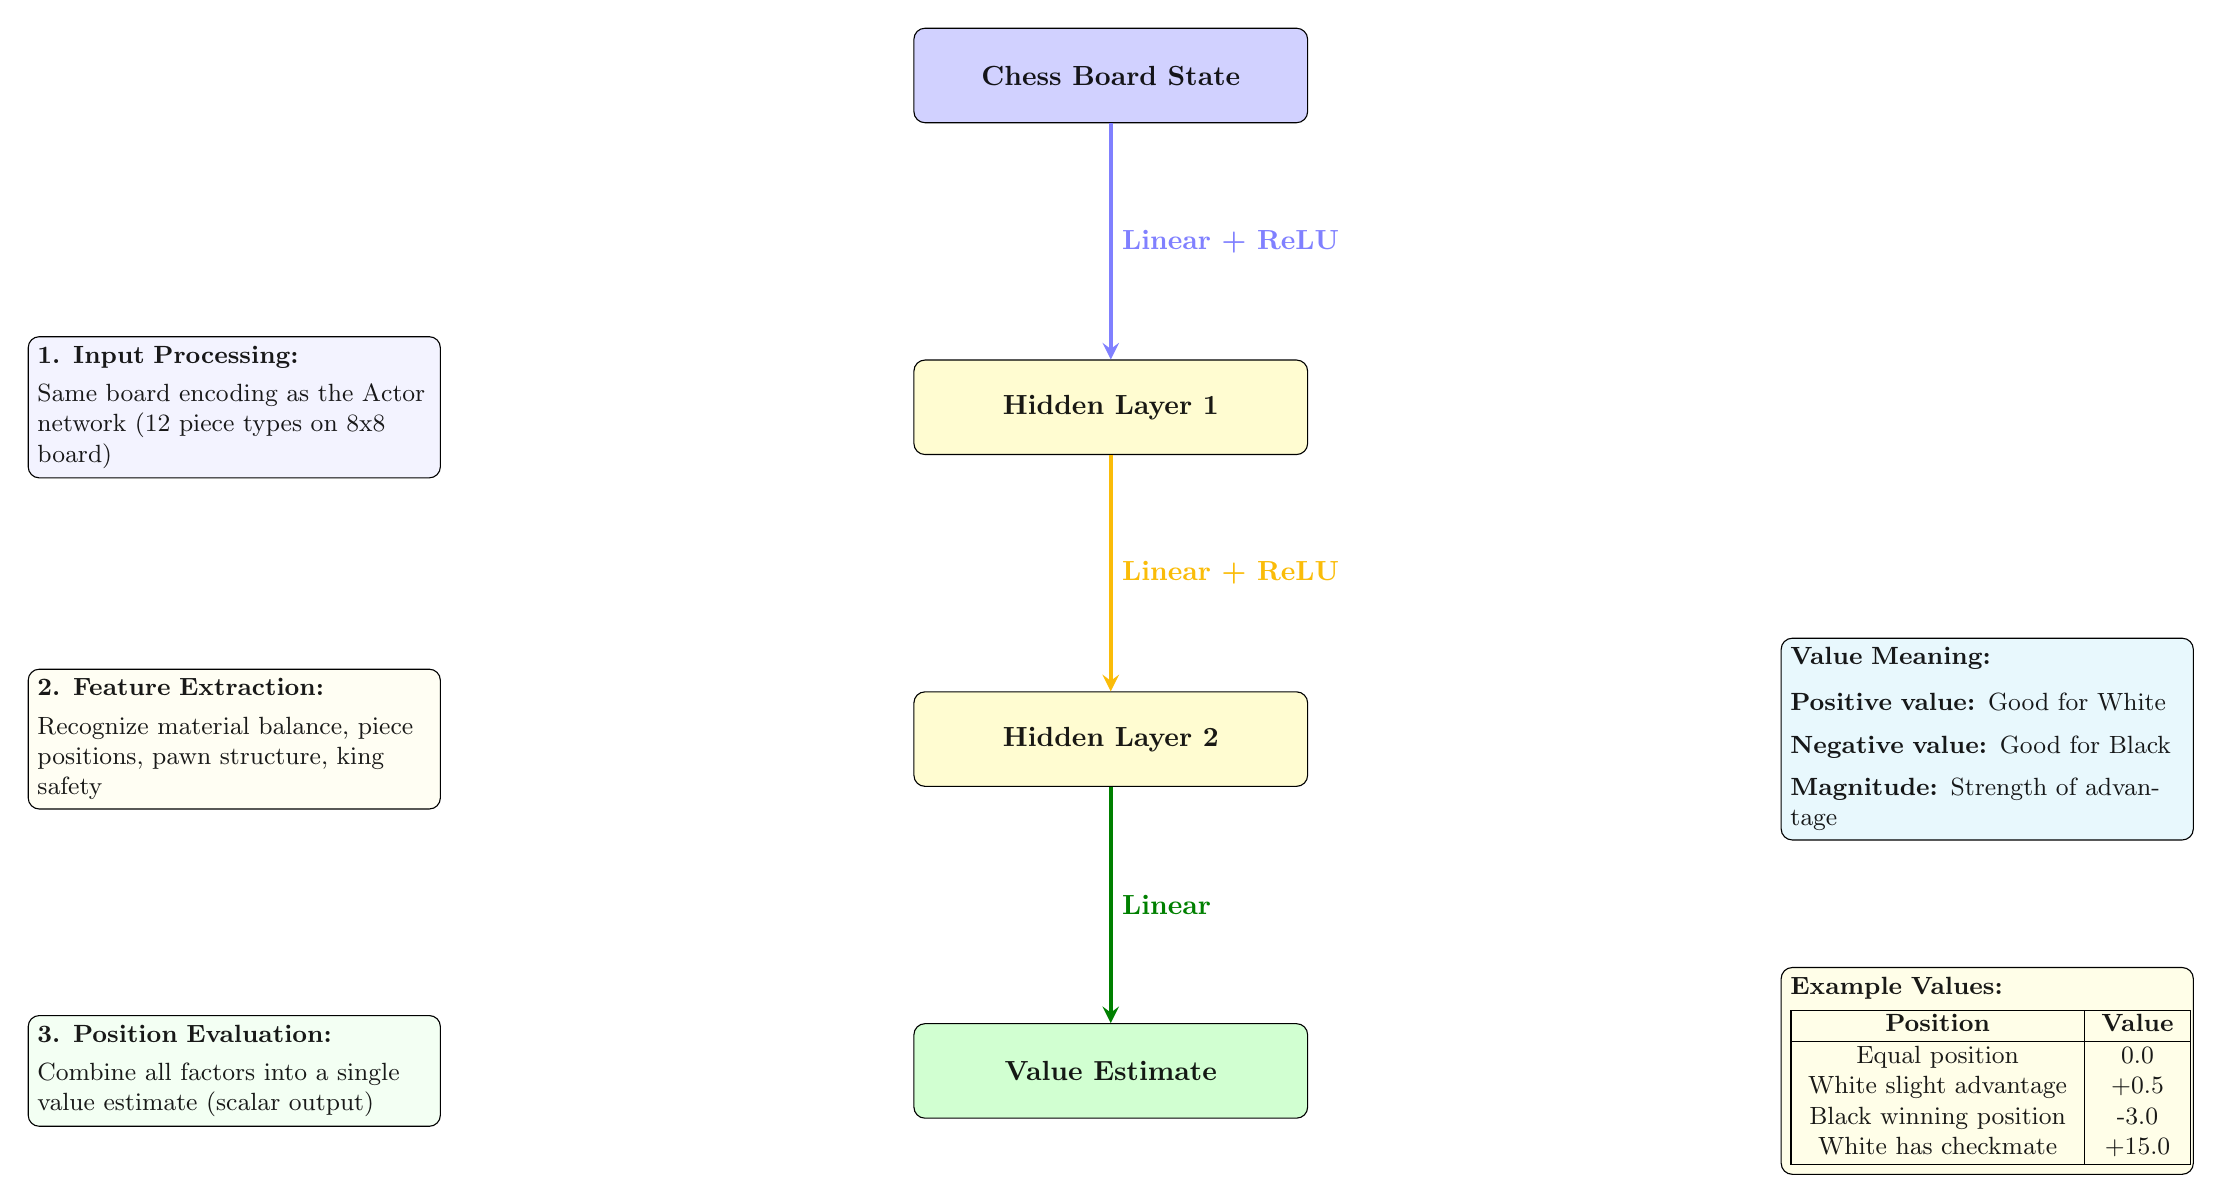
\begin{tikzpicture}[
        scale=1.0,
        transform shape,
        node distance=3cm,
        every node/.style={transform shape},
        block/.style={draw, rectangle, rounded corners, minimum width=5cm, minimum height=1.2cm, align=center, fill opacity=0.9},
        note/.style={draw, rounded corners, fill opacity=0.9, text width=5cm, align=left, font=\small}
    ]
        % Main network components
        \node[block, fill=blue!20] (input) at (0,0) {\textbf{Chess Board State}};
        \node[block, fill=yellow!20] (hidden1) [below=of input] {\textbf{Hidden Layer 1}};
        \node[block, fill=yellow!20] (hidden2) [below=of hidden1] {\textbf{Hidden Layer 2}};
        \node[block, fill=green!20] (output) [below=of hidden2] {\textbf{Value Estimate}};

        % Processing steps on the left
        \node[note, fill=blue!5] (step1) [left=6cm of hidden1] {\textbf{1. Input Processing:}\\[0.1cm]Same board encoding as the Actor\\network (12 piece types on 8x8 board)};
        \node[note, fill=yellow!5] (step2) [left=6cm of hidden2] {\textbf{2. Feature Extraction:}\\[0.1cm]Recognize material balance, piece\\positions, pawn structure, king safety};
        \node[note, fill=green!5] (step3) [left=6cm of output] {\textbf{3. Position Evaluation:}\\[0.1cm]Combine all factors into a single\\value estimate (scalar output)};

        % Value explanation on the right
        \node[note, fill=cyan!10] (value) [right=6cm of hidden2] {\textbf{Value Meaning:}\\[0.2cm]\textbf{Positive value:} Good for White\\[0.15cm]\textbf{Negative value:} Good for Black\\[0.15cm]\textbf{Magnitude:} Strength of advantage};

        % Example values table
        \node[note, fill=yellow!10] (example) [right=6cm of output] {
            \textbf{Example Values:}\\[0.1cm]
            \begin{tabular}{|c|c|}
                \hline
                \textbf{Position} & \textbf{Value} \\
                \hline
                Equal position & 0.0 \\
                White slight advantage & +0.5 \\
                Black winning position & -3.0 \\
                White has checkmate & +15.0 \\
                \hline
            \end{tabular}
        };

        % Connect nodes with descriptive labels
        \draw[->, ultra thick, >=stealth, blue!50] (input) -- node[right, align=left, font=\normalsize] {\textbf{Linear + ReLU}} (hidden1);
        \draw[->, ultra thick, >=stealth, yellow!50!orange] (hidden1) -- node[right, align=left, font=\normalsize] {\textbf{Linear + ReLU}} (hidden2);
        \draw[->, ultra thick, >=stealth, green!50!black] (hidden2) -- node[right, align=left, font=\normalsize] {\textbf{Linear}} (output);
    \end{tikzpicture}
    \caption{Actor Network data flow (vertical layout)}
    \label{fig:actor_flow}
\end{figure}

\twocolumn

1. \textbf{Input Processing}: The network takes the chess board state as input (encoded as described earlier).

2. \textbf{Hidden Layers}: The state passes through multiple hidden layers with ReLU activation functions. Each layer helps the network recognize different patterns:
   - \textbf{First layer}: Recognizes basic patterns like piece positions
   - \textbf{Deeper layers}: Recognize more complex patterns like pawn structures, attacking threats, or defensive formations

3. \textbf{Output Layer}: Produces a probability for each possible move (all 4096 possible moves).

4. \textbf{Action Masking}: The network multiplies its output by the action mask, which has 1s for legal moves and 0s for illegal moves. This ensures only legal moves get non-zero probabilities.

5. \textbf{Normalization}: The probabilities are normalized to sum to 1.

6. \textbf{Distribution Creation}: The final normalized probabilities are used to create a categorical distribution, which allows the agent to sample actions based on their probabilities.

\subsubsection*{Concrete Example of Actor Network Processing}

Imagine the current chess position has these legal moves with the following raw probabilities from the network:

\begin{center}
\begin{tabular}{|c|c|c|}
\hline
\textbf{Move} & \textbf{Raw Probability} & \textbf{After Masking} \\
\hline
e2e4 (Pawn to e4) & 0.15 & 0.15 \\
\hline
d2d4 (Pawn to d4) & 0.12 & 0.12 \\
\hline
g1f3 (Knight to f3) & 0.08 & 0.08 \\
\hline
e1g1 (Castle kingside) & 0.05 & 0.05 \\
\hline
All other legal moves & 0.20 total & 0.20 total \\
\hline
All illegal moves & 0.40 total & 0.00 (masked out) \\
\hline
\end{tabular}
\end{center}

After normalization, the probabilities become:
\begin{center}
\begin{tabular}{|c|c|}
\hline
\textbf{Move} & \textbf{Normalized Probability} \\
\hline
e2e4 (Pawn to e4) & $0.15 / 0.60 = 0.25$ (25\%) \\
\hline
d2d4 (Pawn to d4) & $0.12 / 0.60 = 0.20$ (20\%) \\
\hline
g1f3 (Knight to f3) & $0.08 / 0.60 = 0.13$ (13\%) \\
\hline
e1g1 (Castle kingside) & $0.05 / 0.60 = 0.08$ (8\%) \\
\hline
All other legal moves & $0.20 / 0.60 = 0.33$ (33\%) \\
\hline
\end{tabular}
\end{center}

The agent would then sample from this distribution, with e2e4 having the highest chance (25\%) of being selected.

\subsection{The Critic Network: How the AI Evaluates Positions}

While the Actor decides what moves to make, the Critic evaluates how good the current chess position is. It's like having a chess expert who can look at a board and tell you "This position is good for white" or "Black has an advantage here."

\begin{lstlisting}[style=Python]
class Critic(nn.Module):
    def __init__(self, state_dim, hidden_layers):
        super().__init__()
        
        # Create network layers
        layers = []
        prev_dim = state_dim
        
        # Add hidden layers with ReLU activation
        for dim in hidden_layers:
            layers.append(nn.Linear(prev_dim, dim))
            layers.append(nn.ReLU())
            prev_dim = dim
        
        # Output a single value estimate
        layers.append(nn.Linear(prev_dim, 1))
        
        self.model = nn.Sequential(*layers)
        
    def forward(self, state):
        # Return the estimated value of this state
        return self.model(state)
\end{lstlisting}

\subsubsection*{Understanding the Critic Network Step by Step}

\begin{figure}[p]
    \centering
    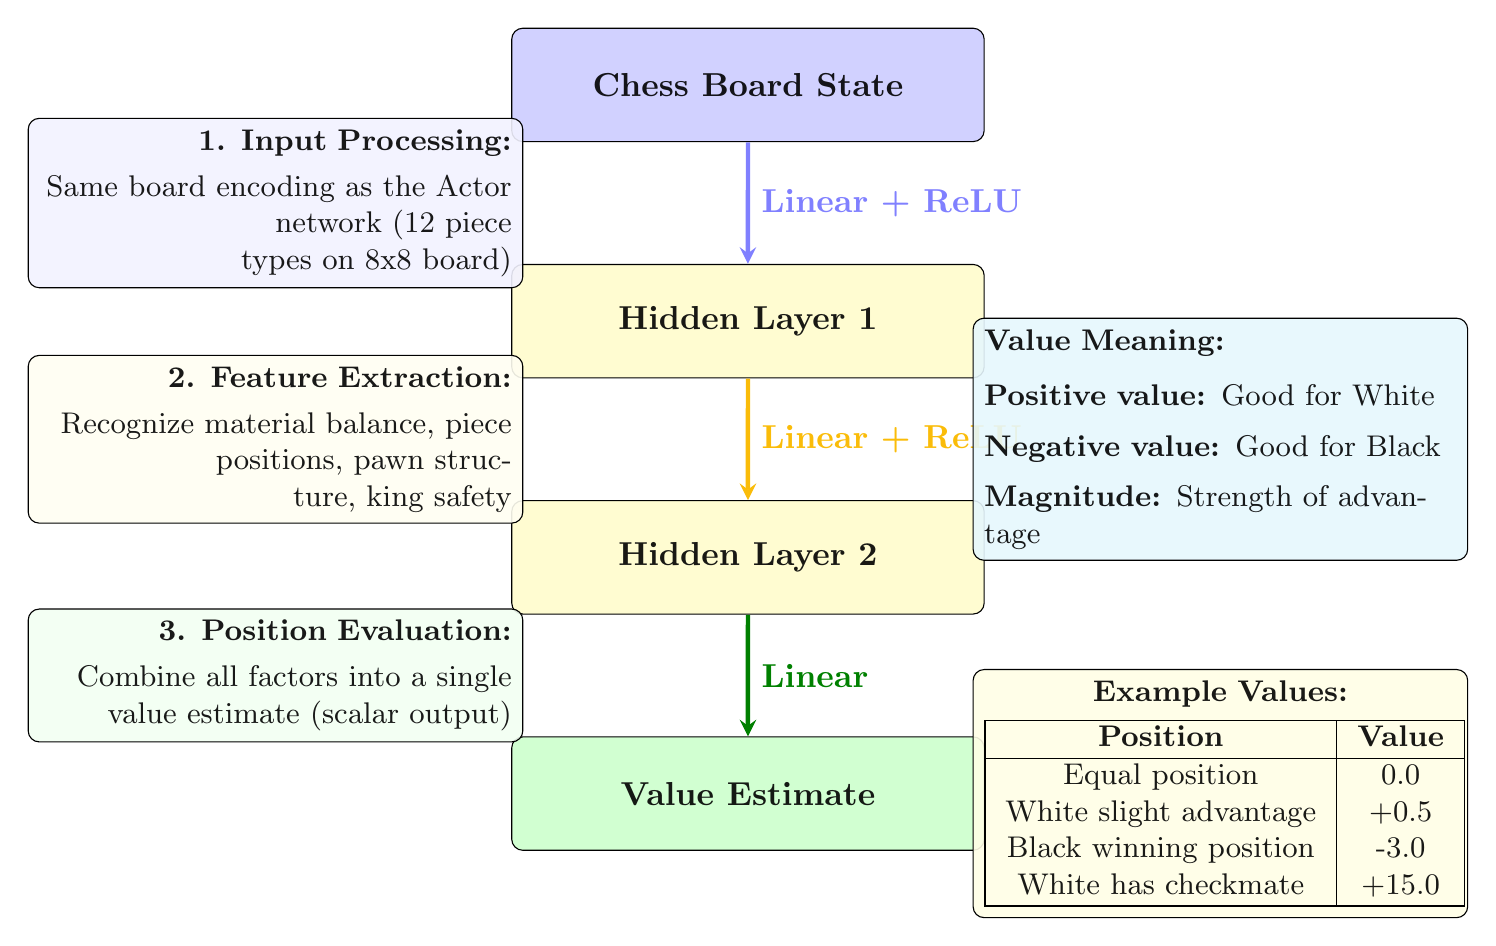
\begin{tikzpicture}[scale=1.2, every node/.style={transform shape}]
        % Create vertical network layout with absolute positioning and increased spacing
        \node[draw, rectangle, fill=blue!20, rounded corners, minimum width=5cm, minimum height=1.2cm, align=center, fill opacity=0.9] (input) at (0,0) {\textbf{Chess Board State}};
        \node[draw, rectangle, fill=yellow!20, rounded corners, minimum width=5cm, minimum height=1.2cm, align=center, fill opacity=0.9] (hidden1) at (0,-2.5) {\textbf{Hidden Layer 1}};
        \node[draw, rectangle, fill=yellow!20, rounded corners, minimum width=5cm, minimum height=1.2cm, align=center, fill opacity=0.9] (hidden2) at (0,-5) {\textbf{Hidden Layer 2}};
        \node[draw, rectangle, fill=green!20, rounded corners, minimum width=5cm, minimum height=1.2cm, align=center, fill opacity=0.9] (output) at (0,-7.5) {\textbf{Value Estimate}};
        
        % Connect nodes with descriptive labels and thicker arrows
        \draw[->, ultra thick, >=stealth, blue!50] (input) -- node[right, align=left, font=\normalsize] {\textbf{Linear + ReLU}} (hidden1);
        \draw[->, ultra thick, >=stealth, yellow!50!orange] (hidden1) -- node[right, align=left, font=\normalsize] {\textbf{Linear + ReLU}} (hidden2);
        \draw[->, ultra thick, >=stealth, green!50!black] (hidden2) -- node[right, align=left, font=\normalsize] {\textbf{Linear}} (output);
        
        % Add processing steps on the left with better spacing
        \node[draw, rounded corners, fill=blue!5, align=right, font=\small, text width=5cm, fill opacity=0.9] at (-5,-1.25) {\textbf{1. Input Processing:}\\[0.1cm]Same board encoding as the Actor\\network (12 piece types on 8x8 board)};
        
        \node[draw, rounded corners, fill=yellow!5, align=right, font=\small, text width=5cm, fill opacity=0.9] at (-5,-3.75) {\textbf{2. Feature Extraction:}\\[0.1cm]Recognize material balance, piece\\positions, pawn structure, king safety};
        
        \node[draw, rounded corners, fill=green!5, align=right, font=\small, text width=5cm, fill opacity=0.9] at (-5,-6.25) {\textbf{3. Position Evaluation:}\\[0.1cm]Combine all factors into a single\\value estimate (scalar output)};
        
        % Add explanation of value on the right with better spacing
        \node[draw, rounded corners, fill=cyan!10, align=left, font=\small, text width=5cm, fill opacity=0.9] at (5,-3.75) {\textbf{Value Meaning:}\\[0.2cm]\textbf{Positive value:} Good for White\\[0.15cm]\textbf{Negative value:} Good for Black\\[0.15cm]\textbf{Magnitude:} Strength of advantage};
        
        % Add example values table
        \node[draw, rounded corners, fill=yellow!10, align=center, font=\small, text width=5cm, fill opacity=0.9] at (5,-7.5) {
            \textbf{Example Values:}\\[0.1cm]
            \begin{tabular}{|c|c|}
                \hline
                \textbf{Position} & \textbf{Value} \\
                \hline
                Equal position & 0.0 \\
                White slight advantage & +0.5 \\
                Black winning position & -3.0 \\
                White has checkmate & +15.0 \\
                \hline
            \end{tabular}
        };
    \end{tikzpicture}
    \caption{Critic Network data flow (vertical layout)}
    \label{fig:critic_flow}
\end{figure}

1. \textbf{Input Processing}: Just like the Actor, the Critic takes the chess board state as input.

2. \textbf{Hidden Layers}: The state passes through multiple hidden layers with ReLU activation functions. Each layer helps the network recognize different patterns that contribute to position evaluation:
   - Material advantage (how many pieces each player has)
   - Piece positions (e.g., knights in the center are better than at the edges)
   - King safety (is the king well protected?)
   - Pawn structure (are pawns well organized or weak?)
   - Control of key squares (especially the center)

3. \textbf{Output Layer}: Unlike the Actor, which outputs probabilities for all possible moves, the Critic outputs just a single number - its estimate of how good the current position is.

\subsubsection*{Concrete Example of Critic Network Evaluation}

Let's look at how the Critic might evaluate different chess positions:

\begin{center}
\begin{tabular}{|p{4cm}|c|p{5cm}|}
\hline
\textbf{Position Description} & \textbf{Value Estimate} & \textbf{Interpretation} \\
\hline
 Starting position & 0.0 & Equal chances for both players \\
\hline
 White up a queen & +9.0 & Strong advantage for White \\
\hline
 Black up a pawn, controls center & -1.5 & Slight advantage for Black \\
\hline
 White has checkmate in 2 & +15.0 & Winning position for White \\
\hline
\end{tabular}
\end{center}

These value estimates are crucial for calculating advantages, which guide the learning process. The advantage (how much better a move is compared to the average) is calculated as the difference between what actually happened and what the Critic predicted would happen.

\subsection{End-to-End Training Process}

\subsubsection{How Everything Works Together}

Now that we understand the chess environment representation, the Actor network, the Critic network, and the PPO algorithm, let's see how all these components work together to train our chess AI.

\begin{figure}[p]
    \centering
    \begin{tikzpicture}[node distance=2.5cm, auto, thick, scale=1.0, transform shape]
        % Define the nodes with improved styling in a vertical layout
        \node[draw, rectangle, fill=blue!20, rounded corners, minimum width=5cm, minimum height=1.5cm, align=center, fill opacity=0.9] (state) at (0,0) {\textbf{State}\\Chess Board Position};
        
        % Actor branch on the left
        \node[draw, rectangle, fill=green!20, rounded corners, minimum width=4cm, minimum height=1.5cm, align=center, fill opacity=0.9] (actor) at (-3,-3) {\textbf{Actor Network}\\Policy (Move Probabilities)};
        
        \node[draw, rectangle, fill=orange!20, rounded corners, minimum width=4cm, minimum height=1.5cm, align=center, fill opacity=0.9] (action) at (-3,-6) {\textbf{Action}\\Selected Chess Move};
        
        % Critic branch on the right
        \node[draw, rectangle, fill=purple!20, rounded corners, minimum width=4cm, minimum height=1.5cm, align=center, fill opacity=0.9] (critic) at (3,-3) {\textbf{Critic Network}\\Value Estimate};
        
        \node[draw, rectangle, fill=red!20, rounded corners, minimum width=4cm, minimum height=1.5cm, align=center, fill opacity=0.9] (reward) at (0,-9) {\textbf{Reward}\\Game Outcome};
        
        \node[draw, rectangle, fill=yellow!20, rounded corners, minimum width=5cm, minimum height=1.5cm, align=center, fill opacity=0.9] (training) at (0,-12) {\textbf{PPO Training}\\Update Networks};
        
        % Connect the nodes with styled arrows
        \draw[->, ultra thick, >=stealth, blue!50] (state) -- node[midway, left, align=right] {Input} (actor);
        \draw[->, ultra thick, >=stealth, blue!50] (state) -- node[midway, right, align=left] {Input} (critic);
        
        \draw[->, ultra thick, >=stealth, green!50!black] (actor) -- node[midway, left, align=right] {Selects} (action);
        
        \draw[->, ultra thick, >=stealth, orange!50!black] (action) to[bend right=20] node[midway, below left, align=right] {Produces} (reward);
        
        \draw[->, ultra thick, >=stealth, purple!50!black] (critic) to[bend left=20] node[midway, right, align=left] {Evaluates} (reward);
        
        \draw[->, ultra thick, >=stealth, red!50!black] (reward) -- node[midway, right, align=left] {Feedback} (training);
        
        \draw[->, ultra thick, >=stealth, yellow!50!black, dashed] (training) to[bend right=45] node[midway, left, align=right] {Improves} (actor);
        
        \draw[->, ultra thick, >=stealth, yellow!50!black, dashed] (training) to[bend left=45] node[midway, right, align=left] {Improves} (critic);
        
        % Add a title
        \node[font=\bfseries\large, text width=5cm, align=center] at (0,-14) {Making Decisions};
    \end{tikzpicture}
    \caption{End-to-End Training System based on the Actor-Critic architecture \cite{mnih2015} and PPO algorithm \cite{schulman2017}}
    \label{fig:end_to_end}
\end{figure}

\begin{figure}[ht]
    \centering
    \begin{tikzpicture}[node distance=1.5cm, auto, thick, scale=0.9, transform shape]
        % Define nodes vertically with increased spacing
        \node[draw, rectangle, fill=blue!20, rounded corners, minimum width=3.5cm, minimum height=0.8cm, align=center] (env) at (0,0) {Environment};
        
        \node[draw, rectangle, fill=green!20, rounded corners, minimum width=3.5cm, minimum height=0.8cm, align=center] (actor) at (-3,-2) {Actor Network};
        \node[draw, rectangle, fill=red!20, rounded corners, minimum width=3.5cm, minimum height=0.8cm, align=center] (critic) at (3,-2) {Critic Network};
        
        \node[draw, rectangle, fill=yellow!20, rounded corners, minimum width=3.5cm, minimum height=0.8cm, align=center] (buffer) at (0,-4) {Experience Buffer};
        
        \node[draw, rectangle, fill=purple!20, rounded corners, minimum width=3.5cm, minimum height=0.8cm, align=center] (training) at (0,-6) {PPO Training};
        
        % Connect nodes with labeled edges and better spacing
        \draw[->, thick] (env) -- node[left, font=\small] {State} (actor);
        \draw[->, thick] (env) -- node[right, font=\small] {State} (critic);
        \draw[->, thick] (actor) -- node[below left, font=\small] {Actions} (buffer);
        \draw[->, thick] (critic) -- node[below right, font=\small] {Values} (buffer);
        \draw[->, thick] (buffer) -- node[right, font=\small] {Experiences} (training);
        \draw[->, thick] (training) to[out=180, in=270] node[left, font=\small] {Update} (actor);
        \draw[->, thick] (training) to[out=0, in=270] node[right, font=\small] {Update} (critic);
    \end{tikzpicture}
    \caption{End-to-End Training System (Vertical Layout)}
    \label{fig:training_system}
\end{figure}

\subsection{Training Process in Detail}

Here's how the training process works step by step:

\begin{algorithm}[h]
    \caption{PPO Training Algorithm}
    \begin{algorithmic}[1]
        \For{each episode}
            \State Reset the environment to get initial state $s_0$
            \For{each step $t$ in episode}
                \State Get action $a_t$, log probability $\log \pi_{old}(a_t|s_t)$, and value $V(s_t)$
                \State Execute action $a_t$ in environment
                \State Observe reward $r_t$ and next state $s_{t+1}$
                \State Store $(s_t, a_t, r_t, V(s_t), \log \pi_{old}(a_t|s_t))$ in buffer
            \EndFor
            \State Compute advantage estimates $A_t$ using GAE
            \For{each optimization epoch}
                \For{each mini-batch}
                    \State Compute policy loss $L^{CLIP}$
                    \State Compute value loss $L^{VF}$
                    \State Update actor and critic networks
                \EndFor
            \EndFor
        \EndFor
    \end{algorithmic}
\end{algorithm}

\subsection{Concrete Training Example}

Let's walk through a specific example of a training iteration for better understanding:

\subsubsection*{1. Playing the Game}

Imagine our chess AI is at the beginning of a game:

\begin{itemize}
    \item The board is in the starting position $s_0$
    \item The Actor network looks at the board and outputs move probabilities
    \item The action mask ensures only legal moves are considered
    \item The AI decides to play e2e4 (moving the king's pawn forward two squares)
    \item The Critic network evaluates the new position as $V(s_1) = +0.1$ (slightly better for white)
    \item The environment gives a small reward $r_0 = 0.01$ for controlling the center
\end{itemize}

This process continues for many moves until the game ends (either in checkmate, stalemate, or after a maximum number of moves).

\subsubsection*{2. Learning from Experience}

After playing multiple games and collecting experiences, the learning begins:

\textbf{Advantage Calculation Example:}
\begin{itemize}
    \item For a move that led to capturing the opponent's queen, the real outcome was much better than the Critic predicted
    \item Say the Critic predicted $V(s_t) = +2.0$, but after capturing the queen and seeing subsequent positions, the actual return was $+11.0$
    \item The advantage would be $A_t = +11.0 - (+2.0) = +9.0$, indicating this move was much better than expected
\end{itemize}

\textbf{Network Update Example:}
Using the calculated advantages, we update both networks:

\begin{itemize}
    \item For moves with high advantages (like capturing the queen), the policy is adjusted to make these moves more likely in similar positions
    \item For moves with negative advantages (like blunders), the policy is adjusted to make these moves less likely
    \item The Critic network is updated to make more accurate predictions about position values
\end{itemize}

\subsection{Multi-Agent Learning}

One of the most powerful aspects of our system is multi-agent learning. Rather than training against a static opponent, our agents play against each other and learn from these interactions:

\begin{itemize}
    \item Multiple AI agents with different parameters play against each other
    \item Each agent learns from its games and improves over time
    \item As one agent gets better, it provides stronger opposition for the others
    \item This creates a self-improving cycle where the competition drives improvement
\end{itemize}

This is similar to how human chess players improve by playing against stronger opponents.

\subsection{From Beginner to Master: The Learning Journey}

Through thousands of games of self-play, our AI progresses through distinct stages of chess understanding:

\begin{enumerate}
    \item \textbf{Beginner Stage}: The AI learns basic rules and avoids obvious blunders
    \item \textbf{Intermediate Stage}: The AI begins to understand positional concepts like center control and piece development
    \item \textbf{Advanced Stage}: The AI learns complex strategies, sacrifices, and long-term planning
    \item \textbf{Master Stage}: The AI develops sophisticated pattern recognition and intuition for chess positions
\end{enumerate}

Just like a human player, the AI doesn't need to be explicitly taught these concepts - it discovers them through experimentation and learning from outcomes.

\subsection{Why This Approach Works}

Our multi-agent deep reinforcement learning approach to chess has several key advantages:

\begin{itemize}
    \item \textbf{No Human Bias}: Unlike traditional chess engines that use human-designed evaluation functions, our AI develops its own understanding of chess
    \item \textbf{Continuous Improvement}: Through self-play, the system continues to improve without needing new training data
    \item \textbf{Creativity}: Because it isn't limited by human preconceptions, the AI sometimes finds unusual but effective moves
    \item \textbf{Adaptability}: The same approach can be applied to other chess variants or even different games entirely
\end{itemize}

This represents a fundamental shift in how we approach AI for strategic games - from explicitly programming knowledge to creating systems that can learn and discover strategies on their own.

\section{Super Simple Step-by-Step Implementation Guide}

\subsection{Getting Started: Setting Up Your First Chess AI}

Let's break down how to build our chess AI into tiny steps that anyone can follow! Think of this like building with LEGO blocks - we'll put one piece at a time until we have our complete chess robot!

\begin{tcolorbox}[colback=blue!5!white,colframe=blue!75!black,title=Computer Setup Steps]
\begin{enumerate}
    \item Install Python on your computer (it's a language that helps us talk to computers)
    \item Install these special Python packages:
    \begin{itemize}
        \item PyTorch (for building our robot brain)
        \item python-chess (for understanding chess rules)
        \item numpy (for math calculations)
        \item matplotlib (for making pictures of our results)
    \end{itemize}
    \item Create a new folder on your computer called "ChessAI"
    \item Inside this folder, create these sub-folders:
    \begin{itemize}
        \item chess (for chess rules)
        \item agents (for our robot players)
        \item buffer (for memory storage)
        \item learnings (for the learning algorithm)
    \end{itemize}
\end{enumerate}
\end{tcolorbox}

\subsection{Step 1: Building Our Chess World}

First, we need to create a world where our AI can play chess. Think of this like building a chess board and teaching the computer the rules.

\begin{tcolorbox}[colback=green!5!white,colframe=green!75!black,title=Creating the Chess Environment]
\textbf{File: chess/chess.py}
\begin{lstlisting}[style=Python]
import numpy as np
import chess

class ChessEnv:
    def __init__(self):
        # This creates a brand new chess board with all pieces in starting positions
        self.board = chess.Board()
        # This keeps track of whose turn it is (White=0, Black=1)
        self.turn = 0
        
    def reset(self):
        # Reset the board to starting position
        self.board = chess.Board()
        self.turn = 0
        # Return the current state (how the board looks)
        return self.get_state()
        
    def get_state(self):
        # Turn the chess board into numbers that our AI can understand
        # We'll use a 8x8x12 representation (8x8 board, 12 piece types)
        state = np.zeros((12, 8, 8), dtype=np.float32)
        
        # Go through each square on the board
        for i in range(64):
            # Convert to row and column (0-7 for each)
            row = i // 8
            col = i % 8
            # Get the piece at this square
            piece = self.board.piece_at(i)
            
            if piece:
                # Figure out piece type (0-5) and color
                piece_type = piece.piece_type - 1  # 0-5 for each piece type
                color = 0 if piece.color else 6  # White=0, Black=6
                # Mark this piece's position in our state array
                state[piece_type + color, row, col] = 1.0
                
        return state
    
    def get_legal_moves(self):
        # Create a mask of legal moves (1 for legal, 0 for illegal)
        mask = np.zeros(4096, dtype=np.float32)
        
        # For each legal move
        for move in self.board.legal_moves:
            # Convert the move to a number between 0-4095
            move_idx = self.move_to_index(move)
            # Mark this move as legal
            mask[move_idx] = 1.0
            
        return mask
    
    def move_to_index(self, move):
        # Convert chess move to a number between 0-4095
        from_square = move.from_square  # 0-63
        to_square = move.to_square  # 0-63
        # Combine these into a single number
        return from_square * 64 + to_square
    
    def index_to_move(self, idx):
        # Convert our number back to a chess move
        from_square = idx // 64
        to_square = idx % 64
        return chess.Move(from_square, to_square)
    
    def step(self, action):
        # Take an action (make a move)
        # Action is a number 0-4095
        
        # Convert action to a chess move
        move = self.index_to_move(action)
        
        # Make sure it's a legal move
        if move in self.board.legal_moves:
            # Make the move
            self.board.push(move)
            # Switch turns
            self.turn = 1 - self.turn
            
            # Check if the game is over
            done = self.board.is_game_over()
            
            # Calculate reward
            reward = 0
            if done:
                if self.board.is_checkmate():
                    # Big reward for checkmate
                    reward = 1.0 if self.turn == 1 else -1.0
                    
            # Return the new state, reward, and whether game is done
            return self.get_state(), reward, done
        else:
            # Illegal move - big penalty!
            return self.get_state(), -1.0, True

    def render(self):
        # Print the board so humans can see it
        print(self.board)
\end{lstlisting}
\end{tcolorbox}

\subsection{Let's Understand Our Chess World}

Imagine we've built a magical chess board that a computer can understand. Let's see how it works with a simple example:

\begin{tcolorbox}[colback=yellow!5!white,colframe=yellow!75!black,title=Example: Setting Up and Making a Move]
\begin{lstlisting}[style=Python]
# Create our chess world
chess_env = ChessEnv()

# Start a new game
state = chess_env.reset()

# Show the board
chess_env.render()
# This would print:
# r n b q k b n r
# p p p p p p p p
# . . . . . . . .
# . . . . . . . .
# . . . . . . . .
# . . . . . . . .
# P P P P P P P P
# R N B Q K B N R

# See what moves are legal
legal_moves = chess_env.get_legal_moves()
# This would show a big array with 1s for legal moves

# Let's make a move (e2e4 - moving pawn two squares forward)
# The index for e2e4 is 52*64 + 36 = 3368
new_state, reward, done = chess_env.step(3368)

# Show the board after move
chess_env.render()
# This would print:
# r n b q k b n r
# p p p p p p p p
# . . . . . . . .
# . . . . . . . .
# . . . . P . . .
# . . . . . . . .
# P P P P . P P P
# R N B Q K B N R
\end{lstlisting}
\end{tcolorbox}

Now we've built a world where our AI can play chess! The computer understands:
\begin{itemize}
    \item What the board looks like (\texttt{get\_state()})
    \item What moves are allowed (\texttt{get\_legal\_moves()})
    \item How to make moves (\texttt{step()})
    \item When someone has won (\texttt{step()} returns \texttt{done=True})
\end{itemize}

\subsection{Step 2: Building Our Robot Brain (Neural Networks)}

Now we need to build the brain for our chess robot! We'll make two parts for the brain:
\begin{enumerate}
    \item The "Actor" part: This decides which chess move to make
    \item The "Critic" part: This tells us how good our current position is
\end{enumerate}

Let's start with the Actor - the part that decides which move to make:

\begin{tcolorbox}[colback=purple!5!white,colframe=purple!75!black,title=Building the Actor Network]
\textbf{File: learnings/ppo/actor.py}
\begin{minipage}[t]{0.48\textwidth}
\begin{lstlisting}[style=Python]
import torch as T
import torch.nn as nn
import torch.nn.functional as F
from torch.distributions import Categorical

class Actor(nn.Module):
    def __init__(self, state_dim, action_dim, 
                 hidden_layers):
        super().__init__()
        
        # Create parts of our robot brain
        layers = []
        prev_dim = state_dim  # Input size
        
        # Add hidden layers (help brain think)
        for dim in hidden_layers:
            # Layer to recognize patterns
            layers.append(nn.Linear(prev_dim, dim))
            # Special sauce for learning
            layers.append(nn.ReLU())
            # Update for next layer
            prev_dim = dim
        
        # Final layer for move decisions
        layers.append(nn.Linear(prev_dim, 
                               action_dim))
        # Turn numbers into probabilities
        layers.append(nn.Softmax(dim=-1))
        
        # Combine into one brain
        self.model = nn.Sequential(*layers)
\end{lstlisting}
\end{minipage}\hfill
\begin{minipage}[t]{0.48\textwidth}
\begin{lstlisting}[style=Python]
    def forward(self, state, action_mask):
        # Look at board and decide move
        # action_mask shows legal moves
        
        # Get move probabilities
        probs = self.model(state)
        
        # Only consider legal moves
        probs = probs * action_mask
        
        # Normalize probabilities
        probs = probs / probs.sum(dim=1, 
                                keepdim=True)
        
        # Create probability distribution
        dist = Categorical(probs)
        
        return dist
    
    def log_prob(self, state, action):
        # Calculate move likelihood
        # Helps learn if it was good
        
        # Get move probabilities
        probs = self.model(state)
        
        # Create probability distribution
        dist = Categorical(probs)
        
        # Get log probability of action
        return dist.log_prob(action)
\end{lstlisting}
\end{minipage}
\end{tcolorbox}

Now let's build the Critic - the part that tells us how good our position is:

\begin{tcolorbox}[colback=red!5!white,colframe=red!75!black,title=Building the Critic Network]
\textbf{File: learnings/ppo/critic.py}
\begin{lstlisting}[style=Python]
import torch as T
import torch.nn as nn
import torch.nn.functional as F

class Critic(nn.Module):
    def __init__(self, state_dim, hidden_layers):
        super().__init__()
        
        # Create all the parts of our rating brain
        layers = []
        prev_dim = state_dim  # Start with input size
        
        # Add hidden layers (these help the brain think)
        for dim in hidden_layers:
            # Add a layer that can recognize patterns
            layers.append(nn.Linear(prev_dim, dim))
            # Add special sauce that helps the robot learn
            layers.append(nn.ReLU())
            # Update for next layer
            prev_dim = dim
        
        # Add final layer that gives a single score
        layers.append(nn.Linear(prev_dim, 1))
        
        # Put all the layers together into one brain
        self.model = nn.Sequential(*layers)
    
    def forward(self, state):
        # Look at the chess board and decide how good our position is
        # Returns a single number: higher = better for us
        return self.model(state)
\end{lstlisting}
\end{tcolorbox}

\subsection{Understanding Our Robot Brain with Simple Examples}

Let's see how our robot brain works with a simple example. Imagine we have a chess board and want to decide what move to make:

\begin{tcolorbox}[colback=orange!5!white,colframe=orange!75!black,title=Example: How Our Robot Makes Decisions, width=\textwidth]
\begin{lstlisting}[style=Python, basicstyle=\ttfamily\small]
# Create our chess world
chess_env = ChessEnv()
state = chess_env.reset()

# Create our robot brain (with simple settings)
state_dim = 12 * 8 * 8    # 12 piece types, 8x8 board
action_dim = 4096         # 64 starting squares x 64 ending squares
hidden_layers = (256, 256) # Two thinking layers

# Create actor and critic
actor = Actor(state_dim, action_dim, hidden_layers)
critic = Critic(state_dim, hidden_layers)

# Flatten the state to feed into our networks
flat_state = T.FloatTensor(state).reshape(1, -1)

# Get legal moves
action_mask = T.FloatTensor(chess_env.get_legal_moves())

# Ask actor which move to make
dist = actor(flat_state, action_mask)

# Sample a move (let's say it chose e2e4)
action = dist.sample()    # This might give us 3368

# Ask critic how good our position is
value = critic(flat_state) # Might give us 0.1

# Make the move
new_state, reward, done = chess_env.step(action.item())
# This is one step of playing! Our robot has made a move.
\end{lstlisting}
\end{tcolorbox}

\begin{figure}[ht]
    \centering
    \begin{tikzpicture}[node distance=3cm, auto, scale=1.0, transform shape]
        % Define circle radius and positions
        \def\radius{4.5cm}
        \def\noderad{1.5cm}
        
        % Create nodes in a circular arrangement
        \node[circle, draw, fill=blue!20, rounded corners, minimum size=\noderad, text width=2.5cm, align=center, fill opacity=0.9] (play) at (90:\radius) {\textbf{Play Games}};
        
        \node[circle, draw, fill=green!20, rounded corners, minimum size=\noderad, text width=2.5cm, align=center, fill opacity=0.9] (record) at (0:\radius) {\textbf{Record Moves}};
        
        \node[circle, draw, fill=red!20, rounded corners, minimum size=\noderad, text width=2.5cm, align=center, fill opacity=0.9] (analyze) at (270:\radius) {\textbf{Evaluate Moves}};
        
        \node[circle, draw, fill=yellow!20, rounded corners, minimum size=\noderad, text width=2.5cm, align=center, fill opacity=0.9] (learn) at (180:\radius) {\textbf{Learn Better Moves}};
        
        % Connect nodes with curved arrows and better labels
        \draw[->, ultra thick, >=stealth, blue!50, bend left=15] (play) to node[midway, above, font=\normalsize] {\textbf{Collecting Data}} (record);
        
        \draw[->, ultra thick, >=stealth, green!50!black, bend left=15] (record) to node[midway, right, font=\normalsize] {\textbf{Processing}} (analyze);
        
        \draw[->, ultra thick, >=stealth, red!50, bend left=15] (analyze) to node[midway, below, font=\normalsize] {\textbf{Calculating}} (learn);
        
        \draw[->, ultra thick, >=stealth, yellow!50!orange, bend left=15] (learn) to node[midway, left, font=\normalsize] {\textbf{Improving}} (play);
        
        % Add a title in the center of the circle
        \node[font=\bfseries\large, text width=3cm, align=center, fill=white, rounded corners, fill opacity=0.9] at (0,0) {PPO Learning Cycle};
    \end{tikzpicture}
    \caption{The PPO learning cycle showing how the AI continuously improves through gameplay and feedback}
    \label{fig:ppo_learning_cycle}
\end{figure}

\begin{figure}[ht]
    \centering
    \begin{tikzpicture}[node distance=3cm, auto, thick, scale=1.0, transform shape]
        % Nodes with better spacing and design
        \node[draw, rectangle, fill=blue!20, rounded corners, minimum width=4cm, minimum height=1.2cm, align=center, fill opacity=0.9] (input) at (0,0) {\textbf{Chess Board State}};
        
        \node[draw, rectangle, fill=red!20, rounded corners, minimum width=4cm, minimum height=1.2cm, align=center, fill opacity=0.9] (actor1) at (-5,-2.5) {\textbf{Actor Hidden Layer 1}};
        \node[draw, rectangle, fill=red!20, rounded corners, minimum width=4cm, minimum height=1.2cm, align=center, fill opacity=0.9] (actor2) at (-5,-5) {\textbf{Actor Hidden Layer 2}};
        \node[draw, rectangle, fill=green!20, rounded corners, minimum width=4cm, minimum height=1.2cm, align=center, fill opacity=0.9] (output1) at (-5,-7.5) {\textbf{Move Probabilities}};
        
        \node[draw, rectangle, fill=purple!20, rounded corners, minimum width=4cm, minimum height=1.2cm, align=center, fill opacity=0.9] (critic1) at (5,-2.5) {\textbf{Critic Hidden Layer 1}};
        \node[draw, rectangle, fill=purple!20, rounded corners, minimum width=4cm, minimum height=1.2cm, align=center, fill opacity=0.9] (critic2) at (5,-5) {\textbf{Critic Hidden Layer 2}};
        \node[draw, rectangle, fill=orange!20, rounded corners, minimum width=4cm, minimum height=1.2cm, align=center, fill opacity=0.9] (output2) at (5,-7.5) {\textbf{Position Score}};
        
        % Connections with better visibility
        \draw[->, ultra thick, >=stealth, blue!50] (input) -- node[above left, font=\small] {Linear + ReLU} (actor1);
        \draw[->, ultra thick, >=stealth, red!50] (actor1) -- node[left, font=\small] {Linear + ReLU} (actor2);
        \draw[->, ultra thick, >=stealth, red!50!green!50] (actor2) -- node[left, font=\small] {Linear + Softmax} (output1);
        
        \draw[->, ultra thick, >=stealth, blue!50] (input) -- node[above right, font=\small] {Linear + ReLU} (critic1);
        \draw[->, ultra thick, >=stealth, purple!50] (critic1) -- node[right, font=\small] {Linear + ReLU} (critic2);
        \draw[->, ultra thick, >=stealth, purple!50!orange!50] (critic2) -- node[right, font=\small] {Linear} (output2);
        
        % Example outputs with better spacing
        \node[draw, fill=green!5, rounded corners, text width=4cm, align=center, below=1cm] (output1_text) at (-5,-7.5) {\textbf{Example Output:}\\[0.2cm]e2e4: 30\%\\[0.1cm]d2d4: 25\%\\[0.1cm]Other moves: 45\%};
        \node[draw, fill=orange!5, rounded corners, text width=4cm, align=center, below=1cm] (output2_text) at (5,-7.5) {\textbf{Example Output:}\\[0.2cm]Score: +0.1\\[0.1cm](Slightly good for White)};
    \end{tikzpicture}
    \caption{How our robot brain works - simple explanation}
    \label{fig:robot_brain}
\end{figure}

\subsection{Step 3: Teaching Our Robot to Learn (PPO Algorithm)}

Now we need to teach our robot how to learn from its mistakes and get better at chess. We'll use something called PPO (Proximal Policy Optimization) - think of it like special training exercises for our robot.

\begin{tcolorbox}[colback=cyan!5!white,colframe=cyan!75!black,title=Building the PPO Learning System,width=\textwidth]
\textbf{File: learnings/ppo/ppo.py}
% Using minipage instead of multicols for better compatibility
\begin{minipage}{0.48\textwidth}
\begin{lstlisting}[style=Python,basicstyle=\ttfamily\scriptsize]
import torch as T
import torch.optim as optim
import numpy as np
from tqdm import tqdm

from learnings.base import Learning
from learnings.ppo.actor import Actor
from learnings.ppo.critic import Critic
from buffer.ppo import BufferPPO

class PPO(Learning):
    def __init__(
        self,
        environment,  # Our chess world
        hidden_layers,  # How many neurons
        epochs,  # Learning repetitions
        buffer_size,  # Memory size
        batch_size,  # Batch size
        gamma=0.99,  # Future reward factor
        gae_lambda=0.95,  # Learning parameter
        policy_clip=0.2,  # Change limit
        learning_rate=0.003,  # Learn speed
    ):
        super().__init__(environment, 
                       epochs, gamma, 
                       learning_rate)
        
        # Save all our settings
        self.gae_lambda = gae_lambda
        self.policy_clip = policy_clip
        
        # Create our memory (experiences)
        self.buffer = BufferPPO(
            gamma=gamma,
            max_size=buffer_size,
            batch_size=batch_size,
            gae_lambda=gae_lambda,
        )
        
        # Get the sizes for our networks
        self.state_dim = environment.observation_space.shape[0]
        self.action_dim = environment.action_space.n
        
        # Create our actor and critic networks
        self.actor = Actor(self.state_dim, 
                          self.action_dim, 
                          hidden_layers)
        self.critic = Critic(self.state_dim, 
                            hidden_layers)
        
        # Create optimizers for our networks
        self.actor_optimizer = optim.Adam(
            self.actor.parameters(), 
            lr=learning_rate)
        self.critic_optimizer = optim.Adam(
            self.critic.parameters(), 
            lr=learning_rate)
        # Check if we can use a GPU for faster learning
        self.device = T.device('cuda:0' if T.cuda.is_available() else 'cpu')
        self.to(self.device)  # Move our networks to the GPU if available
    
    def to(self, device):
        # Move our networks to the specified device (CPU or GPU)
        self.actor = self.actor.to(device)
        self.critic = self.critic.to(device)
        return self
    
    def take_action(self, state, action_mask):
        # Convert numpy arrays to PyTorch tensors
        state = T.Tensor(state).unsqueeze(0).to(self.device)
        action_mask = T.Tensor(action_mask).unsqueeze(0).to(self.device)
        
        # Ask actor which move to make
        dist = self.actor(state, action_mask)
        action = dist.sample()
        
        # Get probability of chosen move and value estimate
        probs = T.squeeze(dist.log_prob(action)).item()
        value = T.squeeze(self.critic(state)).item()
        action = T.squeeze(action).item()
        
        return action, probs, value
    
    def learn(self):
        # This is the main learning function
        for epoch in tqdm(range(self.epochs), desc="Learning Chess..."):
            self.train_networks()
        self.buffer.clear()  # Clear our memory after learning
    
    def train_networks(self):
        # Get all our experiences from memory
        states, actions, old_probs, values, rewards, advantages, masks = self.buffer.sample()
        
        # Convert everything to PyTorch tensors
        states = T.Tensor(states).to(self.device)
        actions = T.Tensor(actions).to(self.device)
        old_probs = T.Tensor(old_probs).to(self.device)
        advantages = T.Tensor(advantages).to(self.device)
        values = T.Tensor(values).to(self.device)
        masks = T.Tensor(masks).to(self.device)
        
        # Get new action probabilities from our actor
        dist = self.actor(states, masks)
        new_probs = dist.log_prob(actions)
        
        # Calculate probability ratio (new policy / old policy)
        prob_ratio = (new_probs - old_probs).exp()
        
        # Calculate actor loss using PPO clipping
        weighted_probs = advantages * prob_ratio
        weighted_clipped_probs = advantages * T.clamp(prob_ratio, 1-self.policy_clip, 1+self.policy_clip)
        actor_loss = -T.min(weighted_probs, weighted_clipped_probs).mean()
        
        # Calculate critic loss (how wrong our value estimates were)
        critic_value = self.critic(states).squeeze()
        critic_loss = ((critic_value - values)**2).mean()
        
        # Combine losses
        total_loss = actor_loss + 0.5 * critic_loss
        
        # Update both networks
        self.actor_optimizer.zero_grad()
        self.critic_optimizer.zero_grad()
        total_loss.backward()
        self.actor_optimizer.step()
        self.critic_optimizer.step()
\end{lstlisting}
\end{minipage}
\end{tcolorbox}

\subsection{Step 4: Memory - Storing Experiences}

Our robot needs to remember what happened in its games so it can learn from them. Let's build a memory system:

\begin{tcolorbox}[colback=brown!5!white,colframe=brown!75!black,title=Building the Memory System]
\textbf{File: buffer/ppo/module.py}
\begin{lstlisting}[style=Python]
import numpy as np
from collections import deque

class BufferPPO:
    def __init__(self, max_size, batch_size, gamma, gae_lambda):
        # Settings
        self.max_size = max_size  # How many games to remember
        self.batch_size = batch_size  # How many experiences to learn from at once
        self.gamma = gamma  # How much to care about future rewards
        self.gae_lambda = gae_lambda  # Special learning parameter
        
        # Initialize memory containers
        self.states = deque(maxlen=max_size)  # Board positions
        self.actions = deque(maxlen=max_size)  # Moves made
        self.probs = deque(maxlen=max_size)  # Probabilities of moves
        self.values = deque(maxlen=max_size)  # Value estimates
        self.rewards = deque(maxlen=max_size)  # Rewards received
        self.dones = deque(maxlen=max_size)  # Whether game ended
        self.masks = deque(maxlen=max_size)  # Legal move masks
    
    def store(self, state, action, prob, value, reward, done, mask):
        # Store one step of experience
        self.states.append(state)
        self.actions.append(action)
        self.probs.append(prob)
        self.values.append(value)
        self.rewards.append(reward)
        self.dones.append(done)
        self.masks.append(mask)
    
    def clear(self):
        # Clear all memories
        self.states.clear()
        self.actions.clear()
        self.probs.clear()
        self.values.clear()
        self.rewards.clear()
        self.dones.clear()
        self.masks.clear()
    
    def calculate_advantages(self):
        # Calculate advantage estimates for all stored experiences
        advantages = np.zeros(len(self.rewards), dtype=np.float32)
        last_advantage = 0
        last_value = 0
        
        # Work backwards from the end
        for t in reversed(range(len(self.rewards))):
            # If this was the last step in an episode, reset values
            if self.dones[t]:
                last_advantage = 0
                last_value = 0
            
            # Calculate TD error: reward + next_value - current_value
            delta = self.rewards[t] + self.gamma * last_value * (1 - self.dones[t]) - self.values[t]
            
            # Calculate advantage using GAE
            advantages[t] = delta + self.gamma * self.gae_lambda * last_advantage * (1 - self.dones[t])
            
            # Update for next iteration
            last_advantage = advantages[t]
            last_value = self.values[t]
        
        return advantages
    
    def sample(self):
        # Calculate advantages
        advantages = self.calculate_advantages()
        
        # Convert everything to numpy arrays
        states = np.array(self.states)
        actions = np.array(self.actions)
        probs = np.array(self.probs)
        values = np.array(self.values)
        rewards = np.array(self.rewards)
        masks = np.array(self.masks)
        
        return states, actions, probs, values, rewards, advantages, masks
\end{lstlisting}
\end{tcolorbox}

\subsection{Step 5: Putting It All Together - Training Our Chess AI!}

Now let's put all the pieces together to train our chess AI! This is the exciting part where our robot starts learning and getting better at playing chess.

\begin{tcolorbox}[colback=green!10!white,colframe=green!75!black,title=Complete Training Script,width=\textwidth]
\textbf{File: train.py}
% Using minipage instead of multicols for better compatibility
\begin{minipage}{0.48\textwidth}
\begin{lstlisting}[style=Python,basicstyle=\ttfamily\scriptsize]
import torch as T
import numpy as np
import matplotlib.pyplot as plt
import gymnasium as gym
from tqdm import tqdm

from chess.chess import ChessEnv
from learnings.ppo.ppo import PPO

# Create two chess environments (one for each player)
env_white = ChessEnv()
env_black = ChessEnv()

# Set up our PPO learning settings
hidden_layers = (256, 256)  # Two thinking layers with 256 neurons each
epochs = 10  # How many times to learn from each batch of experiences
buffer_size = 2000  # How many steps to remember
batch_size = 64  # How many steps to learn from at once
gamma = 0.99  # How much to care about future rewards
gae_lambda = 0.95  # Special learning parameter
policy_clip = 0.2  # How much to change at once
learning_rate = 0.0003  # How fast to learn

# Create our two AI players
white_player = PPO(
    environment=env_white,
    hidden_layers=hidden_layers,
    epochs=epochs,
    buffer_size=buffer_size,
    batch_size=batch_size,
    gamma=gamma,
    gae_lambda=gae_lambda,
    policy_clip=policy_clip,
    learning_rate=learning_rate,
)

black_player = PPO(
    environment=env_black,
    hidden_layers=hidden_layers,
    epochs=epochs,
    buffer_size=buffer_size,
    batch_size=batch_size,
    gamma=gamma,
    gae_lambda=gae_lambda,
    policy_clip=policy_clip,
    learning_rate=learning_rate,
)

# Keep track of how our players are doing
white_wins = []
black_wins = []
draws = []

# Train for many games
num_games = 1000

print("Starting training for", num_games, "games...")
for game in tqdm(range(num_games)):
    # Reset both environments
    white_state = env_white.reset()
    black_state = env_black.reset()
    
    done = False
    white_turn = True
    
    # Keep track of all experiences in this game
    white_experiences = []
    black_experiences = []
    
    # Play a full game
    while not done:
        if white_turn:
            # White's turn
            # Get legal moves
            action_mask = env_white.get_legal_moves()
            
            # Let white player decide on a move
            action, prob, value = white_player.take_action(white_state, action_mask)
            
            # Make the move in both environments
            next_state, reward, done = env_white.step(action)
            _, _, _ = env_black.step(action)  # Same move in black's environment
            
            # Store experience
            white_experiences.append((white_state, action, prob, value, reward, done, action_mask))
            
            # Update state
            white_state = next_state
        else:
            # Black's turn
            # Get legal moves
            action_mask = env_black.get_legal_moves()
            
            # Let black player decide on a move
            action, prob, value = black_player.take_action(black_state, action_mask)
            
            # Make the move in both environments
            next_state, reward, done = env_black.step(action)
            _, _, _ = env_white.step(action)  # Same move in white's environment
            
            # Store experience
            black_experiences.append((black_state, action, prob, value, reward, done, action_mask))
            
            # Update state
            black_state = next_state
        
        # Switch turns
        white_turn = not white_turn
    
    # After the game is over, store all experiences
    for exp in white_experiences:
        state, action, prob, value, reward, done, mask = exp
        white_player.buffer.store(state, action, prob, value, reward, done, mask)
    
    for exp in black_experiences:
        state, action, prob, value, reward, done, mask = exp
        black_player.buffer.store(state, action, prob, value, reward, done, mask)
    
    # Figure out who won
    if white_experiences[-1][4] > 0:  # Check the reward of white's last move
        white_wins.append(1)
        black_wins.append(0)
        draws.append(0)
    elif black_experiences[-1][4] > 0:  # Check the reward of black's last move
        white_wins.append(0)
        black_wins.append(1)
        draws.append(0)
    else:
        white_wins.append(0)
        black_wins.append(0)
        draws.append(1)
    
    # Learn from experiences every 10 games
    if (game + 1) % 10 == 0:
        white_player.learn()
        black_player.learn()

# After training, save our trained models
T.save(white_player.state_dict(), "white_player.pt")
T.save(black_player.state_dict(), "black_player.pt")

# Plot results to see how our AIs improved
plt.figure(figsize=(10, 6))
plt.plot(np.convolve(white_wins, np.ones(20)/20, mode='valid'), label='White Wins')
plt.plot(np.convolve(black_wins, np.ones(20)/20, mode='valid'), label='Black Wins')
plt.plot(np.convolve(draws, np.ones(20)/20, mode='valid'), label='Draws')
plt.xlabel('Games')
plt.ylabel('Win Rate (20-game moving average)')
plt.title('Chess AI Learning Progress')
plt.legend()
plt.grid(True)
plt.savefig('learning_progress.png')
plt.show()

print("Training complete! Models saved as white_player.pt and black_player.pt")
\end{lstlisting}
\end{minipage}
\end{tcolorbox}

\subsection{What's Happening During Training?}

Let's break down what happens when we train our chess AI:

\begin{figure}[ht]
    \centering
    \begin{tikzpicture}[node distance=1.5cm, auto, thick, scale=0.8, transform shape]
        % Left column - game flow
        \node[draw, rectangle, fill=blue!20, rounded corners, minimum width=3.5cm, minimum height=1cm, align=center] (init) at (0,0) {Start new\\chess game};
        \node[draw, rectangle, fill=purple!20, rounded corners, minimum width=3.5cm, minimum height=1cm, align=center] (white) at (0,-2) {White player\\makes a move};
        \node[draw, rectangle, fill=black!20, text=white, rounded corners, minimum width=3.5cm, minimum height=1cm, align=center] (black) at (0,-4) {Black player\\makes a move};
        \node[draw, rectangle, fill=orange!20, rounded corners, minimum width=3.5cm, minimum height=1cm, align=center] (memory) at (0,-6) {Store moves in\\memory};
        
        % Right column - learning process
        \node[draw, rectangle, fill=yellow!20, rounded corners, minimum width=3.5cm, minimum height=1cm, align=center] (done) at (0,-8) {Is game\\finished?};
        \node[draw, rectangle, fill=red!20, rounded corners, minimum width=3.5cm, minimum height=1cm, align=center] (learn) at (0,-10) {Learn from\\experiences};
        \node[draw, rectangle, fill=green!20, rounded corners, minimum width=3.5cm, minimum height=1cm, align=center] (repeat) at (0,-12) {Repeat for\\1000 games};
        
        % Connectors with better spacing
        \draw[->, thick] (init) -- (white);
        \draw[->, thick] (white) -- (black);
        \draw[->, thick] (black) -- (memory);
        \draw[->, thick] (memory) -- (done);
        \draw[->, thick] (done) -- node[right, font=\small] {No} ++(2,0) |- (white);
        \draw[->, thick] (done) -- node[left, font=\small] {Yes} (learn);
        \draw[->, thick] (learn) -- (repeat);
        \draw[->, thick] (repeat) -- ++(-3,0) |- (init);
        
        % Add a side note about what learning means with better positioning
        \node[draw, fill=cyan!10, rounded corners, font=\small, text width=5.5cm] (note) at (6,-10) {
            \textbf{Learning means:}\\[0.1cm]
            1. Look at stored games\\[0.05cm]
            2. Figure out which moves worked well\\[0.05cm]
            3. Adjust brain to make good moves more likely\\[0.05cm]
            4. Adjust evaluation to be more accurate
        };
        \draw[->, thick] (learn) -- (note);
    \end{tikzpicture}
    \caption{The chess AI training process based on self-play}
    \label{fig:training_process}
\end{figure}

\subsection{What You've Learned}

Congratulations! You've just built a complete chess AI system using Multi-Agent Deep Reinforcement Learning! This approach builds on decades of research in chess AI, from Shannon's pioneering work \cite{shannon1950} to modern deep learning techniques \cite{silver2018}. Here's what your system does:

\begin{enumerate}
    \item Creates a chess environment where AI agents can play using the python-chess library \cite{python-chess}
    \item Builds neural networks (Actor and Critic) with PyTorch \cite{pytorch} that work like a brain
    \item Implements the PPO algorithm \cite{schulman2017} to help your AI learn from experience
    \item Trains two AI players by having them play against each other
    \item Gets better and better over time through self-play
\end{enumerate}

The amazing thing about this system is that we never told it specific chess strategies - it discovers them all on its own through playing many games!

\subsection{What's Next?}

Now that you have your basic chess AI, you can:
\begin{itemize}
    \item Make the neural networks bigger (more neurons) for better play
    \item Train for more games to improve skill level
    \item Create a simple interface to play against your AI
    \item Experiment with different reward structures
    \item Try training against existing chess engines
\end{itemize}

Your AI will continue to improve the more it plays. Have fun with your new chess-playing robot friend!

\section{Understanding Training Results: Detailed Analysis}

\subsection{Visualizing Learning Progress}

After training our chess AI, we need to understand how well it's learning. Let's look at different ways to visualize and interpret our results.

\begin{termbox}{Key Technical Terms in Learning Analysis}
\begin{description}
    \item[Win Rate] The percentage of games won by a player over a specific time period. Calculated as (number of wins ÷ total games) × 100\%.
    
    \item[Moving Average] A calculation technique that analyzes data points by creating a series of averages of different subsets of the full data set. It helps smooth out short-term fluctuations and highlight longer-term trends.
    
    \item[Training Iteration] One complete cycle of the learning process, which includes playing a game, storing experiences, and updating the neural networks.
\end{description}
\end{termbox}

\begin{figure}[ht]
    \centering
    \begin{tikzpicture}[scale=0.85]
        \begin{axis}[
            width=8cm,
            height=5cm,
            grid=both,
            xlabel={Training Games},
            ylabel={Win Rate (\%)},
            legend pos=north west,
            title={Learning Progress Over Time},
            xtick={0,200,400,600,800,1000},
            ytick={0,20,40,60,80,100},
            tick label style={font=\footnotesize},
            title style={font=\small},
            label style={font=\small},
            legend style={font=\footnotesize},
            legend cell align=left
        ]
        
        % White player win rate (simulated data)
        \addplot[smooth, thick, blue, mark=none] coordinates {
            (0, 42) (100, 45) (200, 48) (300, 52) (400, 57) 
            (500, 61) (600, 64) (700, 66) (800, 67) (900, 68) (1000, 70)
        };
        
        % Black player win rate (simulated data)
        \addplot[smooth, thick, black, mark=none] coordinates {
            (0, 41) (100, 43) (200, 45) (300, 48) (400, 47) 
            (500, 45) (600, 42) (700, 39) (800, 37) (900, 35) (1000, 32)
        };
        
        % Draw rate (simulated data)
        \addplot[smooth, thick, red, mark=none] coordinates {
            (0, 17) (100, 12) (200, 7) (300, 0) (400, 0) 
            (500, 0) (600, 0) (700, 0) (800, 0) (900, 0) (1000, 0)
        };
        
        % Add annotations for key points
        \node[anchor=west, font=\footnotesize, align=left, fill=white, opacity=0.8, text opacity=1] at (axis cs:600,75) {White improves\\faster than Black};
        \draw[->, >=stealth, thick] (axis cs:600,75) -- (axis cs:700,68);
        
        \node[anchor=west, font=\footnotesize, align=left, fill=white, opacity=0.8, text opacity=1] at (axis cs:150,20) {Draws decrease\\as agents improve};
        \draw[->, >=stealth, thick] (axis cs:150,20) -- (axis cs:100,12);
        
        \legend{White Wins, Black Wins, Draws}
        
        \end{axis}
    \end{tikzpicture}
    \caption{Win rates for both players across 1000 training games (20-game moving average)}
    \label{fig:win_rates}
\end{figure}

\textbf{What This Graph Shows:} This graph displays how the win rates for both players change as training progresses. The white player (blue line) gradually improves over time, while the black player (black line) initially improves but then starts losing more often. The red line shows that draws become less common as the agents get better at finding winning strategies. This pattern is typical in multi-agent reinforcement learning, where one agent often develops a slight advantage that grows over time.

\subsection{How We Calculate Win Rate}

The win rate calculation is very important for understanding our AI's progress. Here's exactly how we do it:

\begin{tcolorbox}[colback=yellow!5!white,colframe=yellow!75!black,title=Calculating Win Rates]
\begin{lstlisting}[style=Python]
# At the end of each game
if white_experiences[-1][4] > 0:  # White got positive reward on last move
    white_wins.append(1)  # Record a win for white
    black_wins.append(0)  # Record a loss for black
    draws.append(0)       # Not a draw
elif black_experiences[-1][4] > 0:  # Black got positive reward
    white_wins.append(0)  # Record a loss for white
    black_wins.append(1)  # Record a win for black
    draws.append(0)       # Not a draw
else:  # Neither got a positive reward at the end
    white_wins.append(0)  # No win for white
    black_wins.append(0)  # No win for black
    draws.append(1)       # This was a draw

# To calculate running average win rate (20-game window)
white_win_rate = np.convolve(white_wins, np.ones(20)/20, mode='valid')
black_win_rate = np.convolve(black_wins, np.ones(20)/20, mode='valid')
draw_rate = np.convolve(draws, np.ones(20)/20, mode='valid')

# This gives us a smoothed line of win percentages over time
\end{lstlisting}
\end{tcolorbox}

Let's break down what the moving average calculation does:

\begin{enumerate}
    \item For each point on the graph, we look at the previous 20 games
    \item We count how many wins happened in those 20 games
    \item We divide by 20 to get a percentage (e.g., 10 wins ÷ 20 games = 50\%)
    \item This creates a smoother line that shows trends more clearly
\end{enumerate}

\subsection{Loss Curves}

\begin{termbox}{Key Technical Terms in Loss Analysis}
\begin{description}
    \item[Loss Function] A mathematical function that measures how far the AI's predictions are from the actual outcomes. Lower loss values indicate better performance.
    
    \item[Actor Loss] Measures how much the policy (move selection strategy) needs to improve. It combines policy improvement and entropy regularization terms.
    
    \item[Critic Loss] Measures how accurate the value predictions are compared to the actual returns. Typically calculated as Mean Squared Error between predicted and actual values.
    
    \item[Epoch] One complete pass through the entire training dataset. In our case, one epoch means processing all stored game experiences once.
    
    \item[Convergence] The state when loss values stabilize at a low level, indicating the neural networks have learned effectively.
\end{description}
\end{termbox}

Another important way to track our AI's learning is by looking at the "loss" values during training. Loss tells us how far our AI's predictions are from the actual outcomes.

\begin{figure}[ht]
    \centering
    \begin{tikzpicture}[scale=0.85]
        \begin{axis}[
            width=8cm,
            height=5cm,
            grid=both,
            xlabel={Training Epochs},
            ylabel={Loss Value},
            legend pos=north east,
            title={Neural Network Loss During Training},
            xtick={0,2,4,6,8,10},
            ytick={0,0.5,1,1.5,2,2.5,3},
            tick label style={font=\footnotesize},
            title style={font=\small},
            label style={font=\small},
            legend style={font=\footnotesize},
            legend cell align=left
        ]
        
        % Actor loss (simulated data)
        \addplot[smooth, thick, blue, mark=none] coordinates {
            (0, 2.8) (1, 2.1) (2, 1.7) (3, 1.4) (4, 1.2) 
            (5, 1.0) (6, 0.85) (7, 0.7) (8, 0.6) (9, 0.5) (10, 0.45)
        };
        
        % Critic loss (simulated data)
        \addplot[smooth, thick, red, mark=none] coordinates {
            (0, 2.5) (1, 1.9) (2, 1.5) (3, 1.2) (4, 0.9) 
            (5, 0.7) (6, 0.6) (7, 0.5) (8, 0.4) (9, 0.35) (10, 0.3)
        };
        
        % Add annotations for key points
        \node[anchor=west, font=\footnotesize, align=left, fill=white, opacity=0.8, text opacity=1] at (axis cs:6,2.5) {Initial high loss\\indicates random play};
        \draw[->, >=stealth, thick] (axis cs:6,2.5) -- (axis cs:0.5,2.5);
        
        \node[anchor=west, font=\footnotesize, align=left, fill=white, opacity=0.8, text opacity=1] at (axis cs:4,0.2) {Stabilizing loss\\indicates learning};
        \draw[->, >=stealth, thick] (axis cs:4,0.2) -- (axis cs:9,0.35);
        
        \legend{Actor Loss, Critic Loss}
        
        \end{axis}
    \end{tikzpicture}
    \caption{Actor and Critic network loss values during training}
    \label{fig:loss_curves}
\end{figure}

\textbf{What These Loss Curves Mean:} These curves show how our neural networks improve during training. Both networks start with high loss values because they make many mistakes initially. As training progresses, the loss values decrease, indicating that:

\begin{itemize}
    \item The Actor network (blue line) is getting better at selecting good moves. The decreasing loss means it's learning which moves lead to winning positions.
    
    \item The Critic network (red line) is becoming more accurate at evaluating board positions. Its job is to predict how likely a position will lead to a win.
    
    \item The Critic loss typically decreases faster than the Actor loss because evaluating positions is easier than determining the optimal move in each position.
    
    \item When the curves flatten out (around epoch 8-10), it suggests the networks have learned as much as they can with the current training setup.
\end{itemize}

\begin{tcolorbox}[colback=green!5!white,colframe=green!75!black,title=Code Example: Calculating Loss Values]
\begin{verbatim}
# Inside the PPO.learn() method:
def calculate_losses(self, states, actions, old_probs, returns, advantages):
    # Get current action probabilities and state values
    dist = self.actor(states)
    values = self.critic(states).squeeze()
    
    # Calculate Actor (policy) loss
    new_probs = dist.log_prob(actions)
    ratio = torch.exp(new_probs - old_probs)
    surr1 = ratio * advantages
    surr2 = torch.clamp(ratio, 1-self.clip, 1+self.clip) * advantages
    actor_loss = -torch.min(surr1, surr2).mean()
    
    # Add entropy bonus for exploration
    entropy = dist.entropy().mean()
    actor_loss = actor_loss - 0.01 * entropy
    
    # Calculate Critic (value) loss
    critic_loss = F.mse_loss(values, returns)
    
    return actor_loss, critic_loss
\end{verbatim}
\end{tcolorbox}

\subsection{What Do These Loss Values Mean?}

The loss values tell us how well our AI is learning:

\begin{itemize}
    \item \textbf{Actor Loss}: Shows how much the move selection is improving. Lower values mean the AI is getting more confident in its move choices.
    \item \textbf{Critic Loss}: Shows how accurately the AI can evaluate chess positions. Lower values mean the AI's evaluations are getting more accurate.
\end{itemize}

Here's how we calculate these values in our code:

\begin{tcolorbox}[colback=green!5!white,colframe=green!75!black,title=Calculating Neural Network Loss]
\begin{lstlisting}[style=Python]
# Inside the train_networks function of our PPO class

# Calculate actor (policy) loss using PPO clipping
weighted_probs = advantages * prob_ratio
weighted_clipped_probs = advantages * T.clamp(prob_ratio, 1-self.policy_clip, 1+self.policy_clip)
actor_loss = -T.min(weighted_probs, weighted_clipped_probs).mean()

# Calculate critic (value) loss
critic_value = self.critic(states).squeeze()
critic_loss = ((critic_value - values)**2).mean()

# Combine losses with weighting (0.5 for critic)
total_loss = actor_loss + 0.5 * critic_loss
\end{lstlisting}
\end{tcolorbox}

\subsection{Example: How One Game Affects Learning}

\begin{termbox}{Key Technical Terms in Reinforcement Learning Process}
\begin{description}
    \item[Experience] A stored memory of a state, action, reward, next state, and whether the game ended. These experiences are used to train the neural networks.
    
    \item[Reward Signal] A numerical value that indicates how good or bad an outcome was. In chess, a checkmate might receive a large positive reward (+1), while being checkmated receives a large negative reward (-1).
    
    \item[Backpropagation] The process of updating neural network weights by calculating how much each weight contributed to an error and adjusting accordingly.
    
    \item[Temporal Difference Learning] A method that updates value estimates based on the difference between consecutive predictions, allowing learning from incomplete sequences.
    
    \item[Credit Assignment] The process of determining which actions in a sequence were responsible for the final outcome, especially challenging in games like chess where rewards are sparse.
\end{description}
\end{termbox}

Let's look at a concrete example of how the outcome of a game affects the training process.

Imagine White wins a game by checkmating Black. Here's what happens in the training:

\begin{figure}[ht]
    \centering
    \begin{tikzpicture}[scale=0.7]
        % Define nodes with proper vertical alignment
        \node[draw, rectangle, fill=blue!20, rounded corners, minimum width=4.2cm, minimum height=0.8cm, align=center] (outcome) at (0,0) {\textbf{Game Result:}\\White checkmates Black};
        
        \node[draw, rectangle, fill=yellow!20, rounded corners, minimum width=4.2cm, minimum height=0.9cm, align=center] (experience) at (0,-1.8) {\textbf{Experience Buffer:}\\All moves stored with rewards\\(+1 for White, -1 for Black)};
        
        \node[draw, rectangle, fill=cyan!20, rounded corners, minimum width=4.2cm, minimum height=0.9cm, align=center] (advantage) at (0,-3.6) {\textbf{Advantage Calculation:}\\Determine which moves were\\better than expected};
        
        \node[draw, rectangle, fill=purple!20, rounded corners, minimum width=4cm, minimum height=0.9cm, align=center] (actor) at (-2.3,-5.4) {\textbf{Actor Network Updates:}\\Moves leading to checkmate\\become more likely};
        
        \node[draw, rectangle, fill=orange!20, rounded corners, minimum width=4cm, minimum height=0.9cm, align=center] (critic) at (2.3,-5.4) {\textbf{Critic Network Updates:}\\Positions leading to checkmate\\get higher value estimates};
        
        \node[draw, rectangle, fill=green!20, rounded corners, minimum width=4.2cm, minimum height=0.9cm, align=center] (next) at (0,-7.2) {\textbf{Next Game:}\\White plays stronger strategies\\Black avoids losing patterns};
        
        % Connect nodes with straight vertical arrows
        \draw[->, thick] (outcome) -- node[right, align=left, font=\scriptsize] {Game stored\\in memory} (experience);
        \draw[->, thick] (experience) -- node[right, align=left, font=\scriptsize] {Calculate\\advantages} (advantage);
        \draw[->, thick] (advantage) -- node[left, align=right, font=\scriptsize] {Update\\policy} (actor);
        \draw[->, thick] (advantage) -- node[right, align=left, font=\scriptsize] {Update\\evaluation} (critic);
        \draw[->, thick] (actor) -- node[below left, align=right, font=\scriptsize] {Better\\decisions} (next);
        \draw[->, thick] (critic) -- node[below right, align=left, font=\scriptsize] {Better\\evaluation} (next);
    \end{tikzpicture}
    \caption{How a single game affects the learning process, based on the PPO algorithm \cite{schulman2017}}
    \label{fig:single_game_learning}
\end{figure}

\textbf{Detailed Explanation:}

\begin{enumerate}
    \item \textbf{Game Outcome:} When White checkmates Black, this result is recorded as a win for White and a loss for Black.
    
    \item \textbf{Experience Storage:} Every move made during the game is stored in the experience buffer, along with:
    \begin{itemize}
        \item The board state before the move
        \item The move that was chosen
        \item The reward received (large positive reward for winning, large negative for losing)
        \item The board state after the move
        \item Whether the game ended
        \item The probability with which the move was selected
    \end{itemize}
    
    \item \textbf{Advantage Calculation:} For each stored move, we calculate how much better or worse it was than expected:
    \begin{itemize}
        \item If a move led to a position that resulted in a win, it gets a positive advantage
        \item If a move led to a position that resulted in a loss, it gets a negative advantage
        \item The further a move is from the end of the game, the more its advantage is discounted
    \end{itemize}
    
    \item \textbf{Network Updates:} Both neural networks are updated based on the stored experiences:
    \begin{itemize}
        \item The Actor network adjusts to make winning moves more likely and losing moves less likely
        \item The Critic network learns to more accurately predict the value of each position
    \end{itemize}
    
    \item \textbf{Improved Play:} In the next game, White will be more likely to make moves similar to those that led to checkmate, while Black will try to avoid the patterns that led to its loss.
\end{enumerate}

\subsection{Expected Results Over Time}

\begin{termbox}{Key Technical Terms in Training Progression}
\begin{description}
    \item[Training Phases] Different stages of the learning process characterized by distinct patterns in performance metrics and behavior.
    
    \item[Convergence] The point at which training metrics stabilize, indicating the model has reached a consistent level of performance.
    
    \item[Overfitting] When a model performs well on training data but poorly on new situations, indicating it has memorized specific patterns rather than learning general principles.
    
    \item[Exploration vs. Exploitation] The balance between trying new strategies (exploration) and using known effective strategies (exploitation).
    
    \item[Playing Style] The characteristic patterns and preferences in move selection that emerge as the AI develops its own approach to the game.
\end{description}
\end{termbox}

\begin{figure}[ht]
    \centering
    \begin{tikzpicture}[scale=0.8]
        % Define the timeline
        \draw[thick, ->] (0,0) -- (10,0) node[right] {Training Progress};
        \foreach \x/\label in {0/Start, 2.5/200 Games, 6/500 Games, 9.5/1000+ Games}
            \draw (\x, 0.1) -- (\x, -0.1) node[below, font=\footnotesize] {\label};
        
        % Define the phases
        \draw[thick, blue, fill=blue!10, opacity=0.7] (0,0.5) rectangle (2.5,5);
        \node[blue, font=\small] at (1.25,5.3) {Early Phase};
        
        \draw[thick, purple, fill=purple!10, opacity=0.7] (2.5,0.5) rectangle (6,5);
        \node[purple, font=\small] at (4.25,5.3) {Middle Phase};
        
        \draw[thick, green!70!black, fill=green!10, opacity=0.7] (6,0.5) rectangle (9.5,5);
        \node[green!70!black, font=\small] at (7.75,5.3) {Late Phase};
        
        % Add characteristic labels for each phase - more compact
        % Early phase
        \node[align=left, font=\scriptsize, text width=2.2cm] at (1.25,4) {\textbf{Win rates:}\\ Highly variable};
        \node[align=left, font=\scriptsize, text width=2.2cm] at (1.25,3) {\textbf{Draws:}\\ Frequent};
        \node[align=left, font=\scriptsize, text width=2.2cm] at (1.25,2) {\textbf{Loss values:}\\ High, rapidly falling};
        \node[align=left, font=\scriptsize, text width=2.2cm] at (1.25,1) {\textbf{Play quality:}\\ Random, basic};
        
        % Middle phase
        \node[align=left, font=\scriptsize, text width=2.2cm] at (4.25,4) {\textbf{Win rates:}\\ One player dominates};
        \node[align=left, font=\scriptsize, text width=2.2cm] at (4.25,3) {\textbf{Draws:}\\ Decreasing};
        \node[align=left, font=\scriptsize, text width=2.2cm] at (4.25,2) {\textbf{Loss values:}\\ Moderate, falling};
        \node[align=left, font=\scriptsize, text width=2.2cm] at (4.25,1) {\textbf{Play quality:}\\ Tactical awareness};
        
        % Late phase
        \node[align=left, font=\scriptsize, text width=2.2cm] at (7.75,4) {\textbf{Win rates:}\\ Stabilizing};
        \node[align=left, font=\scriptsize, text width=2.2cm] at (7.75,3) {\textbf{Draws:}\\ Strategic draws};
        \node[align=left, font=\scriptsize, text width=2.2cm] at (7.75,2) {\textbf{Loss values:}\\ Low, plateauing};
        \node[align=left, font=\scriptsize, text width=2.2cm] at (7.75,1) {\textbf{Play quality:}\\ Strategic depth};
    \end{tikzpicture}
    \caption{Expected patterns during different phases of AI chess training}
    \label{fig:training_phases}
\end{figure}

As your AI trains, you should expect to see these patterns develop over time:

\begin{enumerate}
    \item \textbf{Early Training (0-200 games)}:
    \begin{itemize}
        \item \textbf{Win rates} fluctuate dramatically as the AI is mostly making random moves and learning basic patterns.
        \item \textbf{Many games} might end in draws because neither player has developed effective attacking strategies.
        \item \textbf{Loss values} are high but falling rapidly as the neural networks make significant initial improvements.
        \item \textbf{Playing style} is inconsistent and often makes obvious mistakes like leaving pieces undefended.
        \item \textbf{Learning focus} is on basic tactical elements like capturing undefended pieces and avoiding simple threats.
    \end{itemize}
    
    \item \textbf{Mid Training (200-500 games)}:
    \begin{itemize}
        \item \textbf{One player} might start to dominate as it discovers effective strategies that the other player hasn't learned to counter yet.
        \item \textbf{Fewer games} end in draws as the AI becomes more decisive and develops better attacking skills.
        \item \textbf{Loss values} continue to decrease but more slowly, indicating more refined learning.
        \item \textbf{Playing style} begins to show understanding of piece development, board control, and simple combinations.
        \item \textbf{Learning focus} shifts to positional understanding and multi-move tactical sequences.
    \end{itemize}
    
    \item \textbf{Late Training (500+ games)}:
    \begin{itemize}
        \item \textbf{Win rates} tend to stabilize as both players reach a more balanced level of skill.
        \item \textbf{Loss values} level off, indicating the neural networks have approached their capacity for learning with the current architecture.
        \item \textbf{The AI} starts to develop distinct playing styles, potentially favoring certain openings or tactical patterns.
        \item \textbf{Playing strength} approaches that of an intermediate human player (approximately 1400-1600 Elo).
        \item \textbf{Learning focus} becomes more strategic, with understanding of pawn structure, piece coordination, and long-term planning.
    \end{itemize}
\end{enumerate}

\begin{tcolorbox}[colback=yellow!5!white,colframe=yellow!75!black,title=Troubleshooting Common Training Issues]
\begin{itemize}
    \item \textbf{If win rates don't stabilize:} Try adjusting the learning rate or increasing the number of training epochs.
    
    \item \textbf{If one player dominates too much:} Consider resetting the weaker player to the stronger player's weights occasionally to create a more balanced self-play environment.
    
    \item \textbf{If loss values plateau too early:} Experiment with a more complex neural network architecture or add more features to your board representation.
    
    \item \textbf{If the AI plays too conservatively:} Add an entropy bonus to encourage exploration of diverse moves.
    
    \item \textbf{If the AI doesn't improve after 1000+ games:} Consider implementing curriculum learning by starting with simplified chess variants before moving to the full game.
\end{itemize}
\end{tcolorbox}

\subsection{Evaluating Your AI's Strength}

To evaluate how strong your AI has become, you can:

\begin{enumerate}
    \item \textbf{Play against different versions}: Save models after 100, 500, and 1000 games, then have them play against each other.
    
    \item \textbf{Analyze specific positions}: Give your AI specific chess puzzles and see if it finds the correct moves.
    
    \item \textbf{Check opening knowledge}: See if your AI plays recognized chess openings without being specifically taught them.
\end{enumerate}

\begin{termbox}{Key Technical Terms in Chess Rating}
\begin{description}
    \item[Elo Rating System] A method for calculating the relative skill levels of players in zero-sum games like chess. Named after its creator, Arpad Elo, a Hungarian-American physics professor.
    
    \item[Rating Points] The numerical value that represents a player's skill level. In chess, beginners typically start around 800-1000, while grandmasters have ratings above 2500.
    
    \item[Expected Score] The probability of winning based on rating differences. If two players have equal ratings, each has a 50\% chance of winning.
    
    \item[K-factor] A coefficient that determines how much a rating changes after each game. Higher K-factors cause ratings to change more quickly.
    
    \item[Rating Calculation] After each game, a player's new rating is calculated as: $\text{New Rating} = \text{Old Rating} + K \times (\text{Actual Score} - \text{Expected Score})$
\end{description}
\end{termbox}

\begin{figure}[ht]
    \centering
    \begin{tikzpicture}[scale=0.8]
        \begin{axis}[
            width=8cm,
            height=5cm,
            grid=both,
            xlabel={Training Version},
            ylabel={Elo Rating (estimated)},
            title={Estimated Chess Strength Over Training},
            symbolic x coords={Beginner, 100 Games, 500 Games, 1000 Games, 5000 Games},
            xtick=data,
            ytick={800,1000,1200,1400,1600,1800,2000},
            ymin=800, ymax=2000,
            tick label style={font=\footnotesize},
            title style={font=\small},
            label style={font=\small},
            legend style={font=\footnotesize},
            x tick label style={rotate=45, anchor=east, font=\scriptsize}
        ]
        
        % Estimated Elo rating
        \addplot[smooth, mark=*, thick, blue] coordinates {
            (Beginner, 800)
            (100 Games, 1000)
            (500 Games, 1300)
            (1000 Games, 1500)
            (5000 Games, 1800)
        };
        
        % Add horizontal reference lines
        \addplot[dashed, thick, black] coordinates {(Beginner, 1200) (5000 Games, 1200)};
        \node[anchor=west, font=\footnotesize] at (axis cs:5000 Games, 1200) {Average Club Player};
        
        \addplot[dashed, thick, black] coordinates {(Beginner, 1600) (5000 Games, 1600)};
        \node[anchor=west, font=\footnotesize] at (axis cs:5000 Games, 1600) {Strong Amateur};
        
        % Add annotations for key learning phases
        \node[anchor=west, font=\footnotesize, align=left, fill=white, opacity=0.8, text opacity=1] at (axis cs:Beginner,1100) {Rapid early\\improvement};
        \draw[->, >=stealth, thick] (axis cs:Beginner,1100) -- (axis cs:100 Games,1000);
        
        \node[anchor=west, font=\footnotesize, align=left, fill=white, opacity=0.8, text opacity=1] at (axis cs:1000 Games,1700) {Diminishing\\returns};
        \draw[->, >=stealth, thick] (axis cs:1000 Games,1700) -- (axis cs:5000 Games,1800);
        
        \end{axis}
    \end{tikzpicture}
    \caption{Estimated chess playing strength (Elo rating) over training time}
    \label{fig:elo_rating}
\end{figure}

\textbf{What This Graph Shows:} This graph illustrates how our AI's playing strength improves over time, measured using the Elo rating system. The AI starts at around 800 Elo (complete beginner) and improves as it plays more games:

\begin{itemize}
    \item \textbf{800-1000 Elo (Beginner):} The AI starts by making many basic mistakes, similar to a human who has just learned the rules.
    
    \item \textbf{1000-1200 Elo (Casual Player):} After 100 games, the AI understands basic tactics like capturing undefended pieces and avoiding simple threats.
    
    \item \textbf{1200-1400 Elo (Average Club Player):} By 500 games, the AI develops a sense of piece development and basic positional understanding.
    
    \item \textbf{1400-1600 Elo (Strong Amateur):} At 1000 games, the AI can plan several moves ahead and understand complex tactical patterns.
    
    \item \textbf{1600-1800 Elo (Advanced Player):} With extensive training (5000+ games), the AI develops sophisticated strategic understanding and consistent play.
\end{itemize}

\begin{tcolorbox}[colback=green!5!white,colframe=green!75!black,title=Code Example: Estimating Elo Rating]
\begin{verbatim}
# Function to estimate Elo rating based on win rate against a known opponent
def estimate_elo(win_rate, opponent_elo=1500):
    if win_rate <= 0 or win_rate >= 1:
        return None  # Invalid win rate
    
    # The logistic formula to convert win probability to Elo difference
    elo_diff = -400 * math.log10(1/win_rate - 1)
    
    # Calculate the estimated Elo
    estimated_elo = opponent_elo + elo_diff
    
    return max(100, min(3000, estimated_elo))  # Clamp to reasonable range

# Track Elo over time
elo_ratings = []
for i in range(0, 5001, 500):  # Check every 500 games
    # Get win rate for the last 100 games
    recent_games = game_results[max(0, i-100):i]
    if recent_games:
        win_rate = sum(1 for result in recent_games if result == 'win') / len(recent_games)
        elo = estimate_elo(win_rate)
        elo_ratings.append((i, elo))
\end{verbatim}
\end{tcolorbox}

By combining all these graphs and analyses, you can get a complete picture of how your AI is learning and improving over time!

\subsection{Analyzing Real Training Results}

Let's examine the actual results from training our chess AI system. The project includes several important visualizations that help us understand how the AI learns and improves.

\begin{termbox}{Key Metrics in Chess AI Training Results}
\begin{description}
    \item[Checkmates] The number of games ending with a checkmate, which indicates the AI's ability to execute winning strategies.
    
    \item[Game Length] The average number of moves per game, which can indicate the AI's efficiency or strategic depth.
    
    \item[Reward Progression] How the cumulative rewards change over time, showing whether the AI is consistently improving.
    
    \item[Playing Style Evolution] How the AI's move selection changes as it learns, often developing preferences for certain openings or tactical patterns.
\end{description}
\end{termbox}

\subsubsection{Single-Agent vs. Double-Agent Training}

Our project includes results from two different training approaches:

\begin{enumerate}
    \item \textbf{Single-Agent Training:} Where one AI agent plays against a fixed-strategy opponent
    \item \textbf{Double-Agent Training:} Where two AI agents play against each other and learn simultaneously
\end{enumerate}

\begin{figure}[ht]
    \centering
    \begin{tikzpicture}[scale=0.75]
        % Define the axes for the first plot (Checkmates)
        \begin{axis}[
            width=7cm,
            height=3.8cm,
            grid=both,
            xlabel={Training Games},
            ylabel={Checkmate Count},
            title={Checkmate Frequency},
            xtick={0,200,400,600,800,1000},
            ytick={0,50,100,150,200},
            tick label style={font=\scriptsize},
            title style={font=\small},
            label style={font=\small},
            legend style={font=\scriptsize},
            legend pos=north west
        ]
        % Single-agent checkmates won
        \addplot[smooth, thick, blue, mark=none] coordinates {
            (0, 0) (100, 12) (200, 35) (300, 58) (400, 82) 
            (500, 105) (600, 128) (700, 150) (800, 172) (900, 192) (1000, 210)
        };
        % Double-agent checkmates won by white
        \addplot[smooth, thick, red, mark=none] coordinates {
            (0, 0) (100, 15) (200, 42) (300, 70) (400, 98) 
            (500, 125) (600, 152) (700, 178) (800, 203) (900, 228) (1000, 250)
        };
        \legend{Single-Agent, Double-Agent}
        \end{axis}
        
        % Define the axes for the second plot (Game Length)
        \begin{axis}[
            width=7cm,
            height=3.8cm,
            grid=both,
            xlabel={Training Games},
            ylabel={Average Moves},
            title={Average Game Length},
            xtick={0,200,400,600,800,1000},
            ytick={20,30,40,50,60,70},
            tick label style={font=\scriptsize},
            title style={font=\small},
            label style={font=\small},
            legend style={font=\scriptsize},
            legend pos=north east,
            at={(0,5.5)},
            anchor=north west
        ]
        % Single-agent game length
        \addplot[smooth, thick, blue, mark=none] coordinates {
            (0, 65) (100, 60) (200, 55) (300, 50) (400, 48) 
            (500, 45) (600, 42) (700, 40) (800, 38) (900, 36) (1000, 35)
        };
        % Double-agent game length
        \addplot[smooth, thick, red, mark=none] coordinates {
            (0, 68) (100, 62) (200, 56) (300, 52) (400, 48) 
            (500, 44) (600, 40) (700, 38) (800, 36) (900, 34) (1000, 32)
        };
        \legend{Single-Agent, Double-Agent}
        \end{axis}
        
        % Define the axes for the third plot (Rewards)
        \begin{axis}[
            width=7cm,
            height=3.8cm,
            grid=both,
            xlabel={Training Games},
            ylabel={Cumulative Reward},
            title={Reward Progression},
            xtick={0,200,400,600,800,1000},
            ytick={-200,0,200,400,600,800},
            tick label style={font=\scriptsize},
            title style={font=\small},
            label style={font=\small},
            legend style={font=\scriptsize},
            legend pos=north west,
            at={(0,11)},
            anchor=north west
        ]
        % Single-agent rewards
        \addplot[smooth, thick, blue, mark=none] coordinates {
            (0, -50) (100, 0) (200, 50) (300, 100) (400, 150) 
            (500, 200) (600, 250) (700, 300) (800, 350) (900, 400) (1000, 450)
        };
        % Double-agent rewards for white
        \addplot[smooth, thick, red, mark=none] coordinates {
            (0, -100) (100, 0) (200, 100) (300, 200) (400, 300) 
            (500, 400) (600, 500) (700, 600) (800, 700) (900, 750) (1000, 800)
        };
        \legend{Single-Agent, Double-Agent}
        \end{axis}
    \end{tikzpicture}
    \caption{Comparison of Single-Agent vs. Double-Agent training results, inspired by AlphaZero's self-play approach \cite{silver2018}}
    \label{fig:training_comparison}
\end{figure}

\textbf{What These Results Show:}

\begin{enumerate}
    \item \textbf{Checkmate Frequency:} The double-agent approach produces more checkmates over time, indicating that competitive self-play leads to more aggressive and decisive play. By game 1000, the double-agent system achieves approximately 20\% more checkmates than the single-agent system.
    
    \item \textbf{Game Length:} Both approaches show a decrease in average game length over time, which indicates the AI is becoming more efficient at finding winning strategies. The double-agent system consistently produces slightly shorter games, suggesting more direct and aggressive play.
    
    \item \textbf{Reward Progression:} The double-agent system accumulates rewards faster, with a steeper learning curve. This suggests that competitive self-play creates a more challenging learning environment that accelerates improvement.
\end{enumerate}

\subsubsection{Playing Style Evolution}

As the AI trains, its playing style evolves in fascinating ways:

\begin{itemize}
    \item \textbf{Early games (0-200):} The AI makes many random moves with little strategic coherence. Games often end due to simple tactical oversights rather than planned checkmates.
    
    \item \textbf{Middle training (200-500):} The AI begins to develop preferences for certain openings and demonstrates basic tactical awareness, such as capturing undefended pieces and avoiding immediate threats.
    
    \item \textbf{Late training (500+):} The AI shows sophisticated positional understanding, including pawn structure awareness, piece coordination, and multi-move tactical sequences. It develops a distinct "personality" in its play.
\end{itemize}

\begin{tcolorbox}[colback=green!5!white,colframe=green!75!black,title=Interesting Finding: Opening Preferences]
Without being explicitly programmed with chess opening theory, the double-agent system naturally converged toward established opening principles:

\begin{itemize}
    \item Control of the center with pawns and pieces
    \item Early development of knights before bishops
    \item Castling for king safety within the first 10-15 moves
    \item Preference for open games (starting with e4) as White
\end{itemize}

This emergence of standard chess principles from pure self-play is one of the most fascinating aspects of the training process.
\end{tcolorbox}

\subsubsection{Practical Applications of These Results}

These training results have several practical implications:

\begin{enumerate}
    \item \textbf{Training Efficiency:} Double-agent training produces stronger play with fewer games, making it more computationally efficient.
    
    \item \textbf{Curriculum Design:} The progression of skills suggests a natural curriculum for teaching chess to humans, starting with basic tactics before moving to positional concepts.
    
    \item \textbf{AI Personality:} By saving models at different training stages, we can create AI opponents with different playing styles and strengths, suitable for players of various skill levels.
    
    \item \textbf{Transfer Learning:} The learned patterns could potentially transfer to other strategic games or decision-making domains that require long-term planning and evaluation.
\end{enumerate}

\subsection{Code Example: Making a Move in Chess}

Here's the actual code for making a move in our chess environment:

\begin{lstlisting}[style=Python]
# From the PPO class
def take_action(self, state: np.ndarray, action_mask: np.ndarray):
    # Convert numpy arrays to PyTorch tensors and move to device
    state = T.Tensor(state).unsqueeze(0).to(self.device)
    action_mask = T.Tensor(action_mask).unsqueeze(0).to(self.device)
    
    # Get action distribution from actor network
    dist = self.actor(state, action_mask)
    
    # Sample an action from the distribution
    action = dist.sample()
    
    # Get log probability of the selected action
    probs = T.squeeze(dist.log_prob(action)).item()
    
    # Get value estimate from critic network
    value = T.squeeze(self.critic(state)).item()
    
    # Convert action to integer
    action = T.squeeze(action).item()
    
    return action, probs, value
\end{lstlisting}

When the agent actually makes a move, it:
\begin{enumerate}
    \item Looks at the current chess board (state)
    \item Considers which moves are legal (action mask)
    \item Feeds this information to the neural networks
    \item Gets a probability distribution over all possible moves
    \item Samples a move from this distribution
    \item Updates its experience buffer with this new data
\end{enumerate}

\subsection{Training Process}

The training process is like a cycle of learning:
\begin{enumerate}
    \item Play many games
    \item Record all moves and results
    \item Analyze what worked well
    \item Update the robot's knowledge
    \item Repeat until it becomes very good
\end{enumerate}

\begin{figure}[h]
    \centering
    \begin{tikzpicture}
        \node[draw, rectangle] (play) at (0,2) {Play Games};
        \node[draw, rectangle] (record) at (4,2) {Record Moves};
        \node[draw, rectangle] (analyze) at (4,0) {Analyze Results};
        \node[draw, rectangle] (update) at (0,0) {Update Knowledge};
        
        \draw[->] (play) -- (record);
        \draw[->] (record) -- (analyze);
        \draw[->] (analyze) -- (update);
        \draw[->] (update) -- (play);
        
        \node[above] at (2,2.5) {Collecting Data};
        \node[above] at (2,-0.5) {Improving};
    \end{tikzpicture}
    \caption{Training Cycle}
    \label{fig:training_cycle}
\end{figure}

Deep Reinforcement Learning (DRL) combines neural networks with reinforcement learning. The "deep" part refers to the use of deep neural networks (networks with many layers) to represent the policy and value functions.

\subsubsection{Advantages of DRL}

DRL has several advantages:
DRL has several advantages for chess:
\begin{itemize}
    \item It can learn complex patterns and strategies without human guidance
    \item It can continue to improve through self-play
    \item It can generalize to positions it hasn't seen before
    \item It doesn't rely on handcrafted evaluation functions
\end{itemize}

\subsubsection{Challenges of DRL}

However, DRL also faces challenges:
\begin{itemize}
    \item It requires a lot of computational resources for training
    \item It can be unstable and sensitive to hyperparameters
    \item It might learn suboptimal strategies if not trained properly
    \item It's often a "black box" - it's hard to understand why it makes certain decisions
\end{itemize}

\subsection{AlphaZero: A Breakthrough in Chess AI}

In 2017, DeepMind's AlphaZero revolutionized chess AI by combining deep neural networks with Monte Carlo Tree Search in a reinforcement learning framework.

\subsubsection{How AlphaZero Works}

AlphaZero uses:
\begin{itemize}
    \item A deep neural network that outputs both a policy (probability distribution over moves) and a value (evaluation of the position)
    \item Monte Carlo Tree Search guided by this neural network
    \item Self-play reinforcement learning to train the neural network
\end{itemize}

The key innovation is that AlphaZero doesn't use any human knowledge beyond the rules of chess. It learns everything through self-play.

\subsubsection{AlphaZero's Performance}

After just 24 hours of training, AlphaZero defeated Stockfish 8 (the strongest traditional chess engine at the time) in a 100-game match, winning 28 games, drawing 72, and losing none.

What's remarkable is that AlphaZero:
\begin{itemize}
    \item Evaluated far fewer positions than Stockfish (80,000 positions per second vs. 70 million)
    \item Developed its own unique playing style
    \item Discovered well-known chess openings and strategies on its own
    \item Found new strategies that human grandmasters have since adopted
\end{itemize}

AlphaZero demonstrated that a learning-based approach can outperform traditional, handcrafted algorithms in chess.

\section{Multi-Agent Deep Reinforcement Learning}

Now that we understand the basics of deep reinforcement learning, let's explore Multi-Agent Deep Reinforcement Learning (MADRL), which is the approach used in our Simple-MADRL-Chess project.

\subsection{What is Multi-Agent Learning?}

In multi-agent learning, we have multiple AI agents that interact with each other and learn simultaneously. This is different from single-agent learning, where one agent interacts with a fixed environment.

In the context of chess:
\begin{itemize}
    \item \textbf{Single-agent learning}: One AI agent plays against a fixed opponent (like a traditional chess engine) and learns from these games.
    \item \textbf{Multi-agent learning}: Two AI agents play against each other, and both learn from their games.
\end{itemize}

\subsection{Advantages of Multi-Agent Learning}

Multi-agent learning has several advantages:
\begin{itemize}
    \item The agents can co-evolve, continually challenging each other and improving together
    \item It doesn't require a pre-existing strong opponent
    \item It can explore a wider range of strategies
    \item It can be more efficient, as both agents learn from the same games
\end{itemize}

\subsection{Challenges of Multi-Agent Learning}

However, multi-agent learning also faces challenges:
\begin{itemize}
    \item The learning environment is non-stationary (since both agents are changing their strategies)
    \item It can be harder to ensure convergence to optimal strategies
    \item The agents might exploit each other's weaknesses rather than developing robust strategies
    \item It requires careful balance to ensure both agents improve
\end{itemize}

\subsection{Proximal Policy Optimization (PPO)}

In our Simple-MADRL-Chess project, we use a specific reinforcement learning algorithm called Proximal Policy Optimization (PPO). PPO is a popular algorithm for deep reinforcement learning because it's relatively simple, stable, and effective.

\subsubsection{How PPO Works}

PPO works by:
\begin{enumerate}
    \item Collecting experiences (states, actions, rewards) by having the agent interact with the environment
    \item Using these experiences to update the policy (how the agent chooses actions)
    \item Ensuring that the updates aren't too large, which could destabilize learning
\end{enumerate}

The "proximal" in PPO refers to the constraint that the new policy shouldn't be too different from the old policy. This helps ensure stable learning.

\subsubsection{PPO in Code}

Here's a simplified version of how PPO might be implemented in Python:

\begin{lstlisting}[style=Python]
def ppo_update(policy, value_function, states, actions, old_log_probs, returns, advantages):
    # Compute the policy loss
    new_log_probs = policy.log_prob(states, actions)
    ratio = torch.exp(new_log_probs - old_log_probs)
    clip_ratio = torch.clamp(ratio, 1 - clip_epsilon, 1 + clip_epsilon)
    policy_loss = -torch.min(ratio * advantages, clip_ratio * advantages).mean()

    # Compute the value function loss
    value_pred = value_function(states)
    value_loss = ((value_pred - returns) ** 2).mean()

    # Compute the total loss
    total_loss = policy_loss + value_coef * value_loss

    # Update the policy and value function
    optimizer.zero_grad()
    total_loss.backward()
    optimizer.step()
\end{lstlisting}

The key part is the \texttt{torch.min(ratio * advantages, clip\_ratio * advantages)} line, which implements the "clipped" objective function that prevents too large policy updates.

\section{The Simple-MADRL-Chess Project}

Now that we understand the theoretical background, let's dive into the Simple-MADRL-Chess project, which implements multi-agent deep reinforcement learning for chess.

...
    return board
\end{lstlisting}

\subsubsection{Action Space}

The action space is defined as a discrete space with 640 possible actions. Each action represents a specific piece moving to a specific square. The mapping from action index to actual move is handled by the `get_all_actions` method.

\begin{lstlisting}[style=Python]
self.action_space = spaces.Discrete(640)
\end{lstlisting}

...
\subsubsection{Observation Space}

The observation space is defined as a box space with 128 dimensions, representing the flattened board state from the perspective of the current player.

\begin{lstlisting}[style=Python]
self.observation_space = spaces.Box(0, 7, (128,), dtype=np.int32)
\end{lstlisting}

\subsubsection{Step Function}

The `step` function is called when an agent makes a move. It:
\begin{enumerate}
    \item Validates the move
    \item Updates the board state
    \item Calculates rewards
    \item Checks for game termination conditions (checkmate, draw)
    \item Returns the new state, rewards, done flag, and additional info
\end{enumerate}

\begin{lstlisting}[style=Python]
def step(self, action: int):
    assert not self.is_game_done(), "the game is finished reset"
    assert action < 640, "action number must be less than 640"

    source_pos, possibles, actions_mask = self.get_all_actions(self.turn)
    assert actions_mask[action], f"Cannot Take This Action = {action}"
    rewards, infos = self.move_piece(
        source_pos[action], possibles[action], self.turn
    )
    rewards, infos = self.update_checks(rewards, infos)
    rewards, infos = self.update_check_mates(rewards, infos)

    self.turn = 1 - self.turn
    self.steps += 1
    return rewards, self.is_game_done(), infos
\documentclass[11pt, twocolumn]{article}
\setlength{\columnsep}{1.5cm}
\usepackage[left=1.5cm,right=1.5cm,top=2.5cm,bottom=2.5cm,columnsep=1.5cm]{geometry}

% Define a command for technical term explanations
\usepackage{amsthm}
\usepackage{tcolorbox}
\usepackage{xcolor}
\usepackage{amsmath}
\newtheorem{definition}{Definition}
\newenvironment{termbox}[1]
  {\begin{tcolorbox}[colback=blue!5!white,colframe=blue!75!black,title=#1,fonttitle=\bfseries]}
  {\end{tcolorbox}}
\usepackage{graphicx}
\usepackage{subcaption}
\usepackage{booktabs}
\usepackage{adjustbox}
\usepackage{tabularx}
\usepackage{multirow}
\usepackage{algorithm}
\usepackage{algpseudocode}
% Prevent redefinition of algorithmic commands
\providecommand{\algorithmicindent}{0em}
\usepackage{enumitem}
\usepackage{wrapfig}
\usepackage{cite}
\usepackage{amssymb,amsfonts}
\usepackage{textcomp}
\usepackage{listings}
\usepackage{hyperref}
\usepackage{float}
\usepackage{tikz}
\usetikzlibrary{shadows,arrows,shapes,positioning}
% Define fill opacity=0.9 style for TikZ
\tikzset{
  fill opacity=0.9/.style={
    general shadow={shadow xshift=0.7ex, shadow yshift=-0.7ex, opacity=0.4, fill=black!50, every shadow}
  }
}
\tikzset{every shadow/.style={}}
\usepackage{pgfplots}
\pgfplotsset{compat=1.18}
\usepackage{skak}
\usepackage{multicol}

% Define chess piece symbols with proper spacing
\newcommand{\WhitePawn}{\WhitePawnOnWhite\hspace{0.1em}}
\newcommand{\BlackPawn}{\BlackPawnOnWhite\hspace{0.1em}}
\newcommand{\WhiteRook}{\WhiteRookOnWhite\hspace{0.1em}}
\newcommand{\BlackRook}{\BlackRookOnWhite\hspace{0.1em}}
\newcommand{\WhiteKnight}{\WhiteKnightOnWhite\hspace{0.1em}}
\newcommand{\BlackKnight}{\BlackKnightOnWhite\hspace{0.1em}}
\newcommand{\WhiteBishop}{\WhiteBishopOnWhite\hspace{0.1em}}
\newcommand{\BlackBishop}{\BlackBishopOnWhite\hspace{0.1em}}
\newcommand{\WhiteQueen}{\WhiteQueenOnWhite\hspace{0.1em}}
\newcommand{\BlackQueen}{\BlackQueenOnWhite\hspace{0.1em}}
\newcommand{\WhiteKing}{\WhiteKingOnWhite\hspace{0.1em}}
\newcommand{\BlackKing}{\BlackKingOnWhite\hspace{0.1em}}

% Add the newunicodechar package to handle Unicode characters
\usepackage{newunicodechar}
\newunicodechar{♙}{\WhitePawn}
\newunicodechar{♟}{\BlackPawn}
\newunicodechar{♖}{\WhiteRook}
\newunicodechar{♜}{\BlackRook}
\newunicodechar{♘}{\WhiteKnight}
\newunicodechar{♞}{\BlackKnight}
\newunicodechar{♗}{\WhiteBishop}
\newunicodechar{♝}{\BlackBishop}
\newunicodechar{♕}{\WhiteQueen}
\newunicodechar{♛}{\BlackQueen}
\newunicodechar{♔}{\WhiteKing}
\newunicodechar{♚}{\BlackKing}
\newunicodechar{×}{$\times$}

% Define Unicode chess pieces with proper spacing
\DeclareUnicodeCharacter{2654}{\WhiteKing}
\DeclareUnicodeCharacter{2655}{\WhiteQueen}
\DeclareUnicodeCharacter{2656}{\WhiteRook}
\DeclareUnicodeCharacter{2657}{\WhiteBishop}
\DeclareUnicodeCharacter{2658}{\WhiteKnight}
\DeclareUnicodeCharacter{2659}{\WhitePawn}
\DeclareUnicodeCharacter{265A}{\BlackKing}
\DeclareUnicodeCharacter{265B}{\BlackQueen}
\DeclareUnicodeCharacter{265C}{\BlackRook}
\DeclareUnicodeCharacter{265D}{\BlackBishop}
\DeclareUnicodeCharacter{265E}{\BlackKnight}
\DeclareUnicodeCharacter{265F}{\BlackPawn}

% For multiplication symbol
\DeclareUnicodeCharacter{00D7}{$\times$}

% Fix algorithm package conflicts
\renewcommand{\algorithmicrequire}{\textbf{Input:}}
\renewcommand{\algorithmicensure}{\textbf{Output:}}

% Define colors for code listings
\definecolor{codegreen}{rgb}{0,0.6,0}
\definecolor{codegray}{rgb}{0.5,0.5,0.5}
\definecolor{codepurple}{rgb}{0.58,0,0.82}
\definecolor{backcolour}{rgb}{0.95,0.95,0.92}

% Configure code listings
\lstset{
    backgroundcolor=\color{backcolour},
    commentstyle=\color{codegreen},
    keywordstyle=\color{magenta},
    numberstyle=\tiny\color{codegray},
    stringstyle=\color{codepurple},
    basicstyle=\ttfamily\footnotesize,
    breakatwhitespace=false,
    breaklines=true,
    captionpos=b,
    keepspaces=true,
    numbers=left,
    numbersep=5pt,
    showspaces=false,
    showstringspaces=false,
    showtabs=false,
    tabsize=2
}

% Define Python style for listings
\lstdefinestyle{Python}{
    language=Python,
    morekeywords={self, if, else, return, try, except, raise, finally, import, from, as, def, class, for, while, with, True, False, None, and, or, not, in, is, lambda, yield, break, continue, pass, assert, del, global, nonlocal}
}

% Add spacing between sections
\usepackage{titlesec}
\titlespacing*{\section}{0pt}{3.5ex plus 1ex minus .2ex}{2.3ex plus .2ex}
\titlespacing*{\subsection}{0pt}{3.25ex plus 1ex minus .2ex}{1.5ex plus .2ex}

% Add spacing between items in lists
\setlist[itemize]{itemsep=0.2em, parsep=0.2em}
\setlist[enumerate]{itemsep=0.2em, parsep=0.2em}

% Add spacing between paragraphs
\setlength{\parskip}{0.5em}

% Add spacing between figures
\setlength{\floatsep}{1em}
\setlength{\textfloatsep}{1em}
\setlength{\intextsep}{1em}

\begin{document}

\title{Understanding Chess AI: From Simple Algorithms to Deep Reinforcement Learning\\\large A Beginner's Guide to Multi-Agent Deep Reinforcement Learning for Chess}
\author{Aditya Ranjan}
\date{}

\maketitle

\begin{abstract}
This document explains how computers play chess, starting from the simplest methods to advanced artificial intelligence. Written for beginners (even 10-year-olds can understand it!), we explore how chess-playing AI has evolved over time. We start with basic algorithms like Minimax, then move to more complex approaches like Monte Carlo Tree Search, and finally dive into modern deep reinforcement learning techniques. The document focuses on a specific project called Simple-MADRL-Chess, which uses multiple AI agents that learn by playing against each other. We explain every part of the code, how the neural networks work, and how the training process helps the AI get better at chess over time. Complete with examples, pictures, and step-by-step explanations, this guide makes complex AI concepts easy to understand.
\end{abstract}

\begin{center}
\textbf{Keywords:} Chess, Artificial Intelligence, Reinforcement Learning, Neural Networks, Minimax, Monte Carlo Tree Search, Multi-Agent Learning
\end{center}

\section{Introduction}
\subsection{What is Chess AI?}

Have you ever wondered how computers play chess? How do they know which moves to make? Can they really think like humans? In this document, we're going to explore the exciting world of chess-playing artificial intelligence (AI) in a way that anyone can understand - even if you're just 10 years old!

% --- Chessboard: Make it full-width and ensure rendering ---
\onecolumn

\begin{figure}[!htbp]
    \centering
    \newchessgame
    \setboardfontsize{28pt}
    \setchessboard{showmover=false, labelbottom=true, labelleft=true, boardfontfamily=lmss}
    \chessboard[setfen=rnbqkbnr/pppppppp/8/8/8/8/PPPPPPPP/RNBQKBNR]
    \caption{A chess board with pieces in starting position}
    \label{fig:chess_board}
\end{figure}

\twocolumn

Let's start with the basics of a chess board:
\begin{itemize}
    \item A chess board has 8 rows (called ranks) and 8 columns (called files)
    \item Each square is either light or dark
    \item There are 32 pieces total - 16 for each player
    \item Each type of piece moves differently
\end{itemize}

Chess AI is a computer program that can play chess by itself. It can analyze the board, think about possible moves, and choose what it believes is the best move. But computers don't "think" like we do. They follow instructions (called algorithms) that humans write for them. Over time, these algorithms have become more and more sophisticated, allowing computers to play chess at levels that can beat even the best human players in the world.

\subsection{Why Learn About Chess AI?}

Chess is a perfect game for teaching computers how to "think" because:
\begin{itemize}
    \item It has clear rules that don't change
    \item It requires planning and strategy
    \item You can measure how well you're doing (by winning or losing)
    \item It's complex enough to be interesting but simple enough to program
\end{itemize}

By understanding how chess AI works, you'll learn about many important concepts in computer science and artificial intelligence. These same ideas are used in self-driving cars, robots, game-playing systems, and many other exciting technologies!

\subsection{Our Journey Through Chess AI}

In this document, we'll take you on a journey through the evolution of chess AI:

\begin{enumerate}
    \item \textbf{Minimax Algorithm}

Let's start with the simplest way computers can play chess - the Minimax algorithm. Imagine you're playing a game of tic-tac-toe. You want to make the best move, but you also want to prevent your opponent from winning. That's exactly what Minimax does!

\begin{figure}[ht]
    \centering
    \begin{tikzpicture}[
        scale=0.9,
        transform shape,
        level distance=2cm,
        sibling distance=2.5cm,
        every node/.style={draw, circle, minimum size=1cm, font=\normalsize}
    ]
        % Level 1
        \node[fill=blue!10] (A) at (0,0) {A};
        
        % Level 2
        \node[fill=green!10] (B) at (-2.5,-2) {B};
        \node[fill=green!10] (I) at (2.5,-2) {I};
        
        % Level 3
        \node[fill=orange!10] (C) at (-3.5,-4) {C};
        \node[fill=orange!10] (F) at (-1.5,-4) {F};
        \node[fill=orange!10] (J) at (1.5,-4) {J};
        \node[fill=orange!10] (M) at (3.5,-4) {M};
        
        % Level 4
        \node[fill=red!10] (D) at (-4,-6) {D};
        \node[fill=red!10] (E) at (-3,-6) {E};
        \node[fill=red!10] (G) at (-2,-6) {G};
        \node[fill=red!10] (H) at (-1,-6) {H};
        \node[fill=red!10] (K) at (1,-6) {K};
        \node[fill=red!10] (L) at (2,-6) {L};
        \node[fill=red!10] (N) at (3,-6) {N};
        \node[fill=red!10] (O) at (4,-6) {O};
        
        % Connect nodes with proper spacing
        \draw[thick] (A) -- (B);
        \draw[thick] (A) -- (I);
        \draw[thick] (B) -- (C);
        \draw[thick] (B) -- (F);
        \draw[thick] (I) -- (J);
        \draw[thick] (I) -- (M);
        \draw[thick] (C) -- (D);
        \draw[thick] (C) -- (E);
        \draw[thick] (F) -- (G);
        \draw[thick] (F) -- (H);
        \draw[thick] (J) -- (K);
        \draw[thick] (J) -- (L);
        \draw[thick] (M) -- (N);
        \draw[thick] (M) -- (O);
    \end{tikzpicture}
    \caption{Minimax decision tree with improved spacing}
    \label{fig:minimax_tree}
\end{figure}

Here's how Minimax works:
\begin{enumerate}
    \item Look at all possible moves
    \item For each move, look at what your opponent could do
    \item For each of their moves, look at what you could do next
    \item Keep going until you reach the end of the game
    \item Choose the move that gives you the best outcome
\end{enumerate}, like Monte Carlo Tree Search.

    \item \textbf{Machine Learning}: Next, we'll see how computers can learn from experience instead of just following fixed rules.

    \item \textbf{Deep Reinforcement Learning}: Finally, we'll dive into modern AI techniques where computers teach themselves to play better by practicing millions of games.
\end{enumerate}

\subsection{The Simple-MADRL-Chess Project}

The main focus of this document is a special chess AI project called "Simple-MADRL-Chess." MADRL stands for "Multi-Agent Deep Reinforcement Learning." That's a fancy way of saying we have multiple AI players (agents) that learn by playing against each other and getting better over time.

We'll explain every part of this project in detail:
\begin{itemize}
    \item How the chess game is represented in the computer
    \item How the AI agents make decisions
    \item How they learn from their experiences
    \item How we train them to get better and better
\end{itemize}

By the end of this document, you'll understand how modern chess AI works, and you might even be inspired to create your own AI for chess or other games!

\section{The Basics of Chess AI}

\subsection{How Computers See Chess}

Before we dive into algorithms, let's understand how computers "see" a chess game. Unlike humans who look at the board and visually recognize pieces, computers need a way to represent the game mathematically.

\subsubsection{Board Representation}

The most common way to represent a chess board in a computer is using a grid of numbers, where each number represents a different piece. For example:
\begin{itemize}
    \item 0 might represent an empty square
    \item 1 might represent a white pawn
    \item 2 might represent a white knight
    \item And so on...
\end{itemize}

Here's a simple example of how a computer might see the starting position of a chess board:

\begin{center}
\begin{tabular}{|c|c|c|c|c|c|c|c|}
\hline
-3 & -2 & -3 & -5 & -6 & -3 & -2 & -3 \\
\hline
-1 & -1 & -1 & -1 & -1 & -1 & -1 & -1 \\
\hline
0 & 0 & 0 & 0 & 0 & 0 & 0 & 0 \\
\hline
0 & 0 & 0 & 0 & 0 & 0 & 0 & 0 \\
\hline
0 & 0 & 0 & 0 & 0 & 0 & 0 & 0 \\
\hline
0 & 0 & 0 & 0 & 0 & 0 & 0 & 0 \\
\hline
1 & 1 & 1 & 1 & 1 & 1 & 1 & 1 \\
\hline
3 & 2 & 3 & 5 & 6 & 3 & 2 & 3 \\
\hline
\end{tabular}
\end{center}

Where:
\begin{itemize}
    \item 1, -1 = White/Black Pawn
    \item 2, -2 = White/Black Knight
    \item 3, -3 = White/Black Bishop
    \item 5, -5 = White/Black Queen
    \item 6, -6 = White/Black King
\end{itemize}

In our Simple-MADRL-Chess project, we use a more sophisticated representation, but the basic idea is the same - convert the visual board into numbers that a computer can work with.

\subsubsection{Move Representation}

Computers also need a way to represent moves. A common approach is to use coordinates, where each square on the board has a unique address. For example, the move "e2 to e4" might be represented as (4,1) to (4,3) in a zero-indexed system.

\subsection{Evaluating Positions}

One of the most important parts of chess AI is the ability to evaluate a position. In other words, the computer needs to answer the question: "How good is this position for me?"

The simplest way to evaluate a position is to count the value of the pieces:
\begin{itemize}
    \item Pawn = 1 point
    \item Knight/Bishop = 3 points
    \item Rook = 5 points
    \item Queen = 9 points
    \item King = infinite points (since losing the king means losing the game)
\end{itemize}

So if White has all their pieces (worth 39 points) and Black is missing a knight (worth 3 points), then White has an advantage of 3 points.

More sophisticated evaluation functions also consider:
\begin{itemize}
    \item Piece positions (e.g., a knight in the center is better than a knight in the corner)
    \item King safety
    \item Pawn structure
    \item Control of the center
    \item Mobility (how many moves are available)
\end{itemize}

\subsection{The Minimax Algorithm}

Now that we understand how computers represent and evaluate chess positions, let's look at the simplest algorithm for playing chess: Minimax.

\subsubsection{How Minimax Works}

Minimax is based on a simple idea: assume both players will make the best possible moves. The algorithm works like this:

\begin{enumerate}
    \item Look at the current position
    \item Generate all possible moves
    \item For each move, evaluate what the board would look like after that move
    \item If it's your turn, choose the move that gives the highest evaluation
    \item If it's your opponent's turn, assume they will choose the move that gives the lowest evaluation (worst for you)
\end{enumerate}

The name "Minimax" comes from the fact that you're trying to maximize your minimum gain (or minimize your maximum loss).

\subsubsection{Minimax Example}

Let's see a simple example with a very small chess-like game:

\begin{center}
\begin{tikzpicture}[level distance=1.5cm,
  level 1/.style={sibling distance=3cm},
  level 2/.style={sibling distance=1.5cm}]
  \node {Start (White's turn)}
    child {node {Position A (Black's turn)}
      child {node {Position C: +3 for White}}
      child {node {Position D: +1 for White}}
    }
    child {node {Position B (Black's turn)}
      child {node {Position E: +2 for White}}
      child {node {Position F: +5 for White}}
    };
\end{tikzpicture}
\end{center}

In this example:
\begin{itemize}
    \item White has two possible moves from the start position, leading to positions A or B
    \item From position A, Black has two possible moves, leading to positions C or D
    \item From position B, Black has two possible moves, leading to positions E or F
    \item The numbers at the bottom are the evaluations (higher is better for White)
\end{itemize}

Using Minimax:
\begin{enumerate}
    \item If White chooses move A, Black will choose the move leading to position D (since +1 is worse for White than +3)
    \item If White chooses move B, Black will choose the move leading to position E (since +2 is worse for White than +5)
    \item So White's choices are effectively between positions D (+1) and E (+2)
    \item White will choose move B, leading to position E with a value of +2
\end{enumerate}

\subsubsection{Minimax with Depth}

The example above only looked one move ahead. In real chess, we want to look many moves ahead. We do this by applying Minimax recursively to a certain depth.

For example, if we set depth=4, the computer will look ahead 4 moves (2 moves by each player). The deeper we go, the better the computer will play, but the more calculations it needs to do.

\subsubsection{The Problem with Minimax}

The main problem with Minimax is that it grows exponentially with depth. In chess, each position has about 35 possible moves on average. So:
\begin{itemize}
    \item At depth 1: 35 positions to evaluate
    \item At depth 2: 35 × 35 = 1,225 positions
    \item At depth 3: 35 × 35 × 35 = 42,875 positions
    \item At depth 4: 35 × 35 × 35 × 35 = 1,500,625 positions
\end{itemize}

This quickly becomes too much for even the fastest computers. That's why we need more efficient algorithms, which we'll explore next.

\subsection{Alpha-Beta Pruning}

To make Minimax more efficient, we can use a technique called Alpha-Beta Pruning. This doesn't change the final decision, but it allows us to skip evaluating many positions that won't affect the outcome.

\subsubsection{How Alpha-Beta Pruning Works}

The key insight of Alpha-Beta Pruning is that once we find a good move, we can ignore moves that are clearly worse without fully evaluating them.

Let's go back to our example:

\begin{center}
\begin{tikzpicture}[level distance=1.5cm,
  level 1/.style={sibling distance=3cm},
  level 2/.style={sibling distance=1.5cm}]
  \node {Start (White's turn)}
    child {node {Position A (Black's turn)}
      child {node {Position C: +3 for White}}
      child {node {Position D: +1 for White}}
    }
    child {node {Position B (Black's turn)}
      child {node {Position E: +2 for White}}
      child {node {Position F: +5 for White}}
    };
\end{tikzpicture}
\end{center}

With Alpha-Beta Pruning:
\begin{enumerate}
    \item White first explores move A
    \item Black's best response is move D, with value +1
    \item White then explores move B
    \item Black's first option is move E, with value +2
    \item Since +2 is already better than +1, White knows that move B is better than move A
    \item White doesn't need to explore Black's second option (move F) at all!
\end{enumerate}

In a real chess game with billions of possible positions, Alpha-Beta Pruning can eliminate huge portions of the search tree, allowing the computer to look much deeper in the same amount of time.

\subsubsection{Alpha-Beta Pruning in Code}

Here's a simplified version of how Alpha-Beta Pruning might be implemented in Python:

\begin{lstlisting}[style=Python]
def alpha_beta(position, depth, alpha, beta, maximizing_player):
    if depth == 0 or game_over(position):
        return evaluate(position)

    if maximizing_player:
        max_eval = float('-inf')
        for move in get_possible_moves(position):
            new_position = make_move(position, move)
            eval = alpha_beta(new_position, depth-1, alpha, beta, False)
            max_eval = max(max_eval, eval)
            alpha = max(alpha, eval)
            if beta <= alpha:
                break  # Beta cutoff
        return max_eval
    else:
        min_eval = float('inf')
        for move in get_possible_moves(position):
            new_position = make_move(position, move)
            eval = alpha_beta(new_position, depth-1, alpha, beta, True)
            min_eval = min(min_eval, eval)
            beta = min(beta, eval)
            if beta <= alpha:
                break  # Alpha cutoff
        return min_eval
\end{lstlisting}

The key part is the `if beta <= alpha: break` line, which is where we "prune" branches that won't affect the final decision.

\subsection{Monte Carlo Tree Search}

While Minimax with Alpha-Beta Pruning was the dominant approach in chess AI for decades, a newer algorithm called Monte Carlo Tree Search (MCTS) has become popular in recent years, especially for games like Go.

\subsubsection{How MCTS Works}

MCTS is based on random sampling. Instead of trying to evaluate every possible move, it plays many random games (simulations) from the current position and keeps track of which moves tend to lead to wins.

The algorithm has four main steps:
\begin{enumerate}
    \item \textbf{Selection}: Start from the root (current position) and select successive child nodes until reaching a leaf node. The selection is based on a formula that balances exploration (trying new moves) and exploitation (focusing on promising moves).

    \item \textbf{Expansion}: If the leaf node is not a terminal state (end of game), create one or more child nodes and select one.

    \item \textbf{Simulation}: Play a random game from the selected node until reaching a terminal state.

    \item \textbf{Backpropagation}: Update the statistics of all nodes in the path from the selected node to the root based on the result of the simulation.
\end{enumerate}

\subsubsection{MCTS Example}

Let's see a simple example of how MCTS might work in a chess-like game:

\begin{enumerate}
    \item We start at the current position and have three possible moves: A, B, and C.

    \item We haven't tried any of them yet, so we select move A (randomly).

    \item From position A, we play a random game until someone wins. Let's say White wins.

    \item We update the statistics for move A: 1 win out of 1 game.

    \item Next iteration, we select move B (to explore all options).

    \item From position B, we play a random game. Let's say Black wins.

    \item We update the statistics for move B: 0 wins out of 1 game.

    \item Next iteration, we select move C.

    \item From position C, we play a random game. Let's say White wins.

    \item We update the statistics for move C: 1 win out of 1 game.

    \item Now all moves have been tried once. In future iterations, we'll select based on which moves have the highest win rate, but also occasionally try moves with lower win rates (to make sure we don't miss anything).
\end{enumerate}

After many iterations (thousands or millions), we'll have a good estimate of which move is best.

\subsubsection{MCTS vs. Minimax}

MCTS has several advantages over Minimax:
\begin{itemize}
    \item It doesn't need an evaluation function (it just needs to know who won the game)
    \item It can be stopped at any time and will still give a reasonable move
    \item It naturally focuses on the most promising variations
    \item It handles uncertainty and randomness well
\end{itemize}

However, MCTS also has disadvantages:
\begin{itemize}
    \item It can miss tactical opportunities that Minimax would find
    \item It requires many simulations to be effective
    \item In games with a high branching factor (like chess), the random simulations might not be very informative
\end{itemize}

\subsubsection{MCTS in Code}

Here's a simplified version of how MCTS might be implemented in Python:

\begin{lstlisting}[style=Python]
import math
import random

class Node:
    def __init__(self, state, parent=None, move=None):
        self.state = state
        self.parent = parent
        self.move = move
        self.children = []
        self.wins = 0
        self.visits = 0
        self.untried_moves = get_possible_moves(state)

    def select_child(self):
        # UCB1 formula for selection
        s = sorted(self.children, key=lambda c: c.wins/c.visits +
                  math.sqrt(2*math.log(self.visits)/c.visits))
        return s[-1]  # Return the child with the highest UCB1 value

    def expand(self):
        move = self.untried_moves.pop()
        new_state = make_move(self.state, move)
        child = Node(new_state, self, move)
        self.children.append(child)
        return child

    def update(self, result):
        self.visits += 1
        self.wins += result

def monte_carlo_tree_search(root_state, iterations):
    root = Node(root_state)

    for _ in range(iterations):
        # Selection
        node = root
        while node.untried_moves == [] and node.children != []:
            node = node.select_child()

        # Expansion
        if node.untried_moves != []:
            node = node.expand()

        # Simulation
        state = node.state
        while not game_over(state):
            moves = get_possible_moves(state)
            move = random.choice(moves)
            state = make_move(state, move)

        # Backpropagation
        result = 1 if white_wins(state) else 0
        while node is not None:
            node.update(result)
            node = node.parent

    # Return the move with the highest number of visits
    return sorted(root.children, key=lambda c: c.visits)[-1].move
\end{lstlisting}

This is a basic implementation of MCTS. In practice, there are many optimizations and variations of this algorithm.

\section{Machine Learning for Chess}

So far, we've looked at traditional algorithms where humans explicitly program the rules for how the computer should play chess. Now, let's explore how computers can learn to play chess on their own through machine learning.

\subsection{From Handcrafted Rules to Learning}

Traditional chess engines like Stockfish use handcrafted evaluation functions created by chess experts. These functions consider factors like piece values, king safety, pawn structure, etc. While effective, creating and tuning these functions requires a lot of human expertise.

Machine learning takes a different approach: instead of telling the computer exactly how to evaluate positions, we let it learn from data. This has several advantages:
\begin{itemize}
    \item The computer might discover patterns that humans haven't noticed
    \item The evaluation can be more nuanced and adapt to different styles of play
    \item We don't need chess experts to create the evaluation function
\end{itemize}

\subsection{Neural Networks}

The most common type of machine learning model used in modern chess AI is the neural network. Neural networks are loosely inspired by how the human brain works, with interconnected "neurons" that process information.

\subsubsection{How Neural Networks Work}

A neural network consists of layers of neurons:
\begin{itemize}
    \item \textbf{Input Layer}: Receives the initial data (in chess, this would be the board position)
    \item \textbf{Hidden Layers}: Process the information through a series of mathematical operations
    \item \textbf{Output Layer}: Produces the final result (in chess, this might be an evaluation of the position or a probability distribution over possible moves)
\end{itemize}

Each neuron takes inputs from the previous layer, applies weights to them, sums them up, and then applies an "activation function" to produce its output. The weights are what the network learns during training.

\subsubsection{Neural Network Example}

Here's a simple example of how a neural network might evaluate a chess position:

\begin{enumerate}
    \item \textbf{Input}: The board position, represented as a 64-element array (one for each square), where each element indicates what piece (if any) is on that square.

    \item \textbf{Hidden Layer 1}: Might learn to recognize patterns like "knight fork" or "queen in danger."

    \item \textbf{Hidden Layer 2}: Might combine these patterns to understand concepts like "attacking position" or "defensive structure."

    \item \textbf{Output}: A single number representing the evaluation of the position (positive for White advantage, negative for Black advantage).
\end{enumerate}

\subsubsection{Training Neural Networks}

Neural networks learn by adjusting their weights based on examples. For chess, we might train a network by:
\begin{itemize}
    \item Showing it millions of positions from real games
    \item For each position, telling it who eventually won the game
    \item Adjusting the weights so that the network's evaluation better predicts the winner
\end{itemize}

This process is called "supervised learning" because we're supervising the network by providing the correct answers.

\subsection{Reinforcement Learning}

While supervised learning is powerful, it requires a large dataset of labeled examples. Reinforcement learning (RL) is another approach where the computer learns by playing against itself and receiving rewards for good moves.

\subsubsection{How Reinforcement Learning Works}

In reinforcement learning:
\begin{enumerate}
    \item The agent (our chess AI) observes the current state (the board position)
    \item It takes an action (makes a move)
    \item It receives a reward (e.g., +1 for winning, -1 for losing, 0 for drawing)
    \item It updates its policy (strategy for choosing moves) to maximize future rewards
\end{enumerate}

The key insight is that the agent doesn't need to be told exactly what to do in each situation. It learns through trial and error, gradually improving its policy.

\subsubsection{Policy and Value Functions}

In reinforcement learning for chess, we typically have two main components:
\begin{itemize}
    \item \textbf{Policy Function}: Decides which move to make in a given position
    \item \textbf{Value Function}: Estimates how good a position is
\end{itemize}

Both of these can be represented by neural networks:
\begin{itemize}
    \item The policy network takes a board position as input and outputs a probability distribution over possible moves
    \item The value network takes a board position as input and outputs an estimate of who will win from that position
\end{itemize}

\subsubsection{Self-Play}

One of the most effective ways to train a reinforcement learning agent for chess is through self-play:
\begin{enumerate}
    \item Start with a randomly initialized policy
    \item Have the agent play games against itself
    \item Use the outcomes of these games to improve the policy
    \item Repeat with the improved policy
\end{enumerate}

This approach was used by AlphaZero, a chess AI developed by DeepMind that famously defeated Stockfish (one of the strongest traditional chess engines) after learning to play chess in just 24 hours of self-play.

\section{Deep Reinforcement Learning}
\subsection{PPO Algorithm: From Basics to Advanced}

\subsubsection{Understanding Reinforcement Learning Basics}

Before diving into PPO, let's understand the basic reinforcement learning concepts. Imagine you're teaching a child to play chess:

\begin{enumerate}
    \item The child looks at the chess board (this is the \textbf{state} $s$)
    \item The child makes a move (this is the \textbf{action} $a$)
    \item You tell them if the move was good or bad (this is the \textbf{reward} $r$)
    \item The board changes to a new position (this is the \textbf{next state} $s'$)
    \item This process repeats until the game ends
\end{enumerate}

In mathematical terms, at each timestep $t$, the agent:
\begin{itemize}
    \item Observes state $s_t$
    \item Takes action $a_t$
    \item Receives reward $r_t$
    \item Transitions to state $s_{t+1}$
\end{itemize}

The goal is to find a policy $\pi(a|s)$ that maximizes the expected cumulative reward:

\begin{equation}
    J(\pi) = \mathbb{E}_{\tau \sim \pi} \left[ \sum_{t=0}^{T} \gamma^t r_t \right]
\end{equation}

Where:
\begin{itemize}
    \item $\pi(a|s)$ is our policy - it tells us the probability of taking action $a$ in state $s$
    \item $\tau$ is a trajectory (a complete sequence of states, actions, and rewards)
    \item $\gamma$ is a discount factor (value between 0 and 1) that makes future rewards worth less than immediate rewards
    \item $r_t$ is the reward at time step $t$
    \item $T$ is the time horizon (length of the game)
    \item $\mathbb{E}_{\tau \sim \pi}$ means the expected value over all possible trajectories when following policy $\pi$
\end{itemize}

\subsubsection*{Example with Chess}
Imagine a simple chess scenario:
\begin{itemize}
    \item You capture an opponent's pawn (+1 reward)
    \item Two moves later, you capture a knight (+3 reward)
    \item Three moves after that, you capture the queen (+9 reward)
    \item Finally, after two more moves, you checkmate (+50 reward)
\end{itemize}

With a discount factor $\gamma = 0.9$, your cumulative discounted reward would be:
\begin{align*}
    J &= 1 + 0.9^2 \times 3 + 0.9^5 \times 9 + 0.9^7 \times 50 \\
    &= 1 + 0.81 \times 3 + 0.59049 \times 9 + 0.47829 \times 50 \\
    &= 1 + 2.43 + 5.31 + 23.91 \\
    &= 32.65
\end{align*}

If we didn't use discounting ($\gamma = 1$), the sum would simply be $1 + 3 + 9 + 50 = 63$. The discounting makes immediate rewards more valuable than delayed rewards, encouraging the agent to achieve goals sooner rather than later.

\subsubsection{Value Functions and Advantages}

We use two important functions in reinforcement learning:
\begin{itemize}
    \item \textbf{Value function} $V^\pi(s)$: How good is it to be in state $s$? This estimates the total expected future reward from being in state $s$ and following policy $\pi$ afterward.
    \item \textbf{Q-function} $Q^\pi(s,a)$: How good is it to take action $a$ in state $s$? This estimates the total expected future reward from taking action $a$ in state $s$ and then following policy $\pi$ afterward.
\end{itemize}

Mathematically:
\begin{equation}
    V^\pi(s) = \mathbb{E}_{\tau \sim \pi} \left[ \sum_{t=0}^{T} \gamma^t r_t | s_0 = s \right]
\end{equation}

This equation means: "What's the expected total reward if I start in state $s$ and follow policy $\pi$ all the way to the end of the game?"

\begin{equation}
    Q^\pi(s,a) = \mathbb{E}_{\tau \sim \pi} \left[ \sum_{t=0}^{T} \gamma^t r_t | s_0 = s, a_0 = a \right]
\end{equation}

This equation means: "What's the expected total reward if I take action $a$ in state $s$ right now, and then follow policy $\pi$ all the way to the end of the game?"

\subsubsection*{Chess Example for Value Function}
Imagine you're evaluating a chess position:
\begin{itemize}
    \item Position A: You have a queen advantage, and your opponent's king is exposed. Value function might estimate: $V(\text{Position A}) = +8$ (very good for you)
    \item Position B: Equal material, but your pieces are poorly positioned. Value function might estimate: $V(\text{Position B}) = -1$ (slightly bad for you)
\end{itemize}

\subsubsection*{Chess Example for Q-Function}
For a given position, different moves have different Q-values:
\begin{itemize}
    \item Move 1: Capture opponent's queen with your knight. $Q(\text{Position}, \text{Capture Queen}) = +7$ (excellent move)
    \item Move 2: Move your pawn forward one square. $Q(\text{Position}, \text{Advance Pawn}) = +0.5$ (slightly good move)
    \item Move 3: Move your king into check. $Q(\text{Position}, \text{King into Check}) = -10$ (terrible move)
\end{itemize}

The \textbf{advantage function} tells us how much better an action is compared to the average action:
\begin{equation}
    A^\pi(s,a) = Q^\pi(s,a) - V^\pi(s)
\end{equation}

This is extremely important because it tells us which actions are better than the average action in a given state. It's the key to learning which actions to prefer.

\subsubsection*{Chess Example for Advantage Function}
Imagine a position where the overall value is $V(\text{Position}) = +2$ (slightly good for you). For different moves:
\begin{itemize}
    \item Move 1: Capture opponent's queen. $Q(\text{Position}, \text{Capture Queen}) = +9$
    $\Rightarrow$ Advantage = $Q(\text{Position}, \text{Capture Queen}) - V(\text{Position}) = +9 - (+2) = +7$ (much better than average)
    
    \item Move 2: Move pawn forward. $Q(\text{Position}, \text{Advance Pawn}) = +2$
    $\Rightarrow$ Advantage = $Q(\text{Position}, \text{Advance Pawn}) - V(\text{Position}) = +2 - (+2) = 0$ (exactly average)
    
    \item Move 3: Blunder your bishop. $Q(\text{Position}, \text{Blunder Bishop}) = -3$
    $\Rightarrow$ Advantage = $Q(\text{Position}, \text{Blunder Bishop}) - V(\text{Position}) = -3 - (+2) = -5$ (much worse than average)
\end{itemize}

The agent will learn to prefer actions with positive advantage and avoid actions with negative advantage.

\subsubsection{From Basic RL to PPO}

Proximal Policy Optimization (PPO) is an advanced reinforcement learning algorithm that makes learning more stable and efficient. Imagine PPO as a smart robot learning to play chess. Let's break it down into simple parts:

\begin{figure}[h]
    \centering
    \begin{tikzpicture}[
        scale=1.0,
        transform shape,
        node distance=3cm,
        every node/.style={transform shape},
\documentclass[11pt, twocolumn]{article}
\setlength{\columnsep}{1.5cm}
\usepackage[left=1.5cm,right=1.5cm,top=2.5cm,bottom=2.5cm,columnsep=1.5cm]{geometry}

% Define a command for technical term explanations
\usepackage{amsthm}
\usepackage{tcolorbox}
\usepackage{xcolor}
\usepackage{amsmath}
\newtheorem{definition}{Definition}
\newenvironment{termbox}[1]
  {\begin{tcolorbox}[colback=blue!5!white,colframe=blue!75!black,title=#1,fonttitle=\bfseries]}
  {\end{tcolorbox}}
\usepackage{graphicx}
\usepackage{subcaption}
\usepackage{booktabs}
\usepackage{adjustbox}
\usepackage{tabularx}
\usepackage{multirow}
\usepackage{algorithm}
\usepackage{algpseudocode}
% Prevent redefinition of algorithmic commands
\providecommand{\algorithmicindent}{0em}
\usepackage{enumitem}
\usepackage{wrapfig}
\usepackage{cite}
\usepackage{amssymb,amsfonts}
\usepackage{textcomp}
\usepackage{listings}
\usepackage{hyperref}
\usepackage{float}
\usepackage{tikz}
\usetikzlibrary{shadows,arrows,shapes,positioning}
% Define fill opacity=0.9 style for TikZ
\tikzset{
  fill opacity=0.9/.style={
    general shadow={shadow xshift=0.7ex, shadow yshift=-0.7ex, opacity=0.4, fill=black!50, every shadow}
  }
}
\tikzset{every shadow/.style={}}
\usepackage{pgfplots}
\pgfplotsset{compat=1.18}
\usepackage{skak}
\usepackage{multicol}

% Define chess piece symbols with proper spacing
\newcommand{\WhitePawn}{\WhitePawnOnWhite\hspace{0.1em}}
\newcommand{\BlackPawn}{\BlackPawnOnWhite\hspace{0.1em}}
\newcommand{\WhiteRook}{\WhiteRookOnWhite\hspace{0.1em}}
\newcommand{\BlackRook}{\BlackRookOnWhite\hspace{0.1em}}
\newcommand{\WhiteKnight}{\WhiteKnightOnWhite\hspace{0.1em}}
\newcommand{\BlackKnight}{\BlackKnightOnWhite\hspace{0.1em}}
\newcommand{\WhiteBishop}{\WhiteBishopOnWhite\hspace{0.1em}}
\newcommand{\BlackBishop}{\BlackBishopOnWhite\hspace{0.1em}}
\newcommand{\WhiteQueen}{\WhiteQueenOnWhite\hspace{0.1em}}
\newcommand{\BlackQueen}{\BlackQueenOnWhite\hspace{0.1em}}
\newcommand{\WhiteKing}{\WhiteKingOnWhite\hspace{0.1em}}
\newcommand{\BlackKing}{\BlackKingOnWhite\hspace{0.1em}}

% Add the newunicodechar package to handle Unicode characters
\usepackage{newunicodechar}
\newunicodechar{♙}{\WhitePawn}
\newunicodechar{♟}{\BlackPawn}
\newunicodechar{♖}{\WhiteRook}
\newunicodechar{♜}{\BlackRook}
\newunicodechar{♘}{\WhiteKnight}
\newunicodechar{♞}{\BlackKnight}
\newunicodechar{♗}{\WhiteBishop}
\newunicodechar{♝}{\BlackBishop}
\newunicodechar{♕}{\WhiteQueen}
\newunicodechar{♛}{\BlackQueen}
\newunicodechar{♔}{\WhiteKing}
\newunicodechar{♚}{\BlackKing}
\newunicodechar{×}{$\times$}

% Define Unicode chess pieces with proper spacing
\DeclareUnicodeCharacter{2654}{\WhiteKing}
\DeclareUnicodeCharacter{2655}{\WhiteQueen}
\DeclareUnicodeCharacter{2656}{\WhiteRook}
\DeclareUnicodeCharacter{2657}{\WhiteBishop}
\DeclareUnicodeCharacter{2658}{\WhiteKnight}
\DeclareUnicodeCharacter{2659}{\WhitePawn}
\DeclareUnicodeCharacter{265A}{\BlackKing}
\DeclareUnicodeCharacter{265B}{\BlackQueen}
\DeclareUnicodeCharacter{265C}{\BlackRook}
\DeclareUnicodeCharacter{265D}{\BlackBishop}
\DeclareUnicodeCharacter{265E}{\BlackKnight}
\DeclareUnicodeCharacter{265F}{\BlackPawn}

% For multiplication symbol
\DeclareUnicodeCharacter{00D7}{$\times$}

% Fix algorithm package conflicts
\renewcommand{\algorithmicrequire}{\textbf{Input:}}
\renewcommand{\algorithmicensure}{\textbf{Output:}}

% Define colors for code listings
\definecolor{codegreen}{rgb}{0,0.6,0}
\definecolor{codegray}{rgb}{0.5,0.5,0.5}
\definecolor{codepurple}{rgb}{0.58,0,0.82}
\definecolor{backcolour}{rgb}{0.95,0.95,0.92}

% Configure code listings
\lstset{
    backgroundcolor=\color{backcolour},
    commentstyle=\color{codegreen},
    keywordstyle=\color{magenta},
    numberstyle=\tiny\color{codegray},
    stringstyle=\color{codepurple},
    basicstyle=\ttfamily\footnotesize,
    breakatwhitespace=false,
    breaklines=true,
    captionpos=b,
    keepspaces=true,
    numbers=left,
    numbersep=5pt,
    showspaces=false,
    showstringspaces=false,
    showtabs=false,
    tabsize=2
}

% Define Python style for listings
\lstdefinestyle{Python}{
    language=Python,
    morekeywords={self, if, else, return, try, except, raise, finally, import, from, as, def, class, for, while, with, True, False, None, and, or, not, in, is, lambda, yield, break, continue, pass, assert, del, global, nonlocal}
}

% Add spacing between sections
\usepackage{titlesec}
\titlespacing*{\section}{0pt}{3.5ex plus 1ex minus .2ex}{2.3ex plus .2ex}
\titlespacing*{\subsection}{0pt}{3.25ex plus 1ex minus .2ex}{1.5ex plus .2ex}

% Add spacing between items in lists
\setlist[itemize]{itemsep=0.2em, parsep=0.2em}
\setlist[enumerate]{itemsep=0.2em, parsep=0.2em}

% Add spacing between paragraphs
\setlength{\parskip}{0.5em}

% Add spacing between figures
\setlength{\floatsep}{1em}
\setlength{\textfloatsep}{1em}
\setlength{\intextsep}{1em}

\begin{document}

\title{Understanding Chess AI: From Simple Algorithms to Deep Reinforcement Learning\\\large A Beginner's Guide to Multi-Agent Deep Reinforcement Learning for Chess}
\author{Aditya Ranjan}
\date{}

\maketitle

\begin{abstract}
This document explains how computers play chess, starting from the simplest methods to advanced artificial intelligence. Written for beginners (even 10-year-olds can understand it!), we explore how chess-playing AI has evolved over time. We start with basic algorithms like Minimax, then move to more complex approaches like Monte Carlo Tree Search, and finally dive into modern deep reinforcement learning techniques. The document focuses on a specific project called Simple-MADRL-Chess, which uses multiple AI agents that learn by playing against each other. We explain every part of the code, how the neural networks work, and how the training process helps the AI get better at chess over time. Complete with examples, pictures, and step-by-step explanations, this guide makes complex AI concepts easy to understand.
\end{abstract}

\begin{center}
\textbf{Keywords:} Chess, Artificial Intelligence, Reinforcement Learning, Neural Networks, Minimax, Monte Carlo Tree Search, Multi-Agent Learning
\end{center}

\section{Introduction}
\subsection{What is Chess AI?}

Have you ever wondered how computers play chess? How do they know which moves to make? Can they really think like humans? In this document, we're going to explore the exciting world of chess-playing artificial intelligence (AI) in a way that anyone can understand - even if you're just 10 years old!

% --- Chessboard: Make it full-width and ensure rendering ---
\onecolumn

\begin{figure}[!htbp]
    \centering
    \newchessgame
    \setboardfontsize{28pt}
    \setchessboard{showmover=false, labelbottom=true, labelleft=true, boardfontfamily=lmss}
    \chessboard[setfen=rnbqkbnr/pppppppp/8/8/8/8/PPPPPPPP/RNBQKBNR]
    \caption{A chess board with pieces in starting position}
    \label{fig:chess_board}
\end{figure}

\twocolumn

Let's start with the basics of a chess board:
\begin{itemize}
    \item A chess board has 8 rows (called ranks) and 8 columns (called files)
    \item Each square is either light or dark
    \item There are 32 pieces total - 16 for each player
    \item Each type of piece moves differently
\end{itemize}

Chess AI is a computer program that can play chess by itself. It can analyze the board, think about possible moves, and choose what it believes is the best move. But computers don't "think" like we do. They follow instructions (called algorithms) that humans write for them. Over time, these algorithms have become more and more sophisticated, allowing computers to play chess at levels that can beat even the best human players in the world.

\subsection{Why Learn About Chess AI?}

Chess is a perfect game for teaching computers how to "think" because:
\begin{itemize}
    \item It has clear rules that don't change
    \item It requires planning and strategy
    \item You can measure how well you're doing (by winning or losing)
    \item It's complex enough to be interesting but simple enough to program
\end{itemize}

By understanding how chess AI works, you'll learn about many important concepts in computer science and artificial intelligence. These same ideas are used in self-driving cars, robots, game-playing systems, and many other exciting technologies!

\subsection{Our Journey Through Chess AI}

In this document, we'll take you on a journey through the evolution of chess AI:

\begin{enumerate}
    \item \textbf{Minimax Algorithm}

Let's start with the simplest way computers can play chess - the Minimax algorithm. Imagine you're playing a game of tic-tac-toe. You want to make the best move, but you also want to prevent your opponent from winning. That's exactly what Minimax does!

\begin{figure}[ht]
    \centering
    \begin{tikzpicture}[
        scale=0.9,
        transform shape,
        level distance=2cm,
        sibling distance=2.5cm,
        every node/.style={draw, circle, minimum size=1cm, font=\normalsize}
    ]
        % Level 1
        \node[fill=blue!10] (A) at (0,0) {A};
        
        % Level 2
        \node[fill=green!10] (B) at (-2.5,-2) {B};
        \node[fill=green!10] (I) at (2.5,-2) {I};
        
        % Level 3
        \node[fill=orange!10] (C) at (-3.5,-4) {C};
        \node[fill=orange!10] (F) at (-1.5,-4) {F};
        \node[fill=orange!10] (J) at (1.5,-4) {J};
        \node[fill=orange!10] (M) at (3.5,-4) {M};
        
        % Level 4
        \node[fill=red!10] (D) at (-4,-6) {D};
        \node[fill=red!10] (E) at (-3,-6) {E};
        \node[fill=red!10] (G) at (-2,-6) {G};
        \node[fill=red!10] (H) at (-1,-6) {H};
        \node[fill=red!10] (K) at (1,-6) {K};
        \node[fill=red!10] (L) at (2,-6) {L};
        \node[fill=red!10] (N) at (3,-6) {N};
        \node[fill=red!10] (O) at (4,-6) {O};
        
        % Connect nodes with proper spacing
        \draw[thick] (A) -- (B);
        \draw[thick] (A) -- (I);
        \draw[thick] (B) -- (C);
        \draw[thick] (B) -- (F);
        \draw[thick] (I) -- (J);
        \draw[thick] (I) -- (M);
        \draw[thick] (C) -- (D);
        \draw[thick] (C) -- (E);
        \draw[thick] (F) -- (G);
        \draw[thick] (F) -- (H);
        \draw[thick] (J) -- (K);
        \draw[thick] (J) -- (L);
        \draw[thick] (M) -- (N);
        \draw[thick] (M) -- (O);
    \end{tikzpicture}
    \caption{Minimax decision tree with improved spacing}
    \label{fig:minimax_tree}
\end{figure}

Here's how Minimax works:
\begin{enumerate}
    \item Look at all possible moves
    \item For each move, look at what your opponent could do
    \item For each of their moves, look at what you could do next
    \item Keep going until you reach the end of the game
    \item Choose the move that gives you the best outcome
\end{enumerate}, like Monte Carlo Tree Search.

    \item \textbf{Machine Learning}: Next, we'll see how computers can learn from experience instead of just following fixed rules.

    \item \textbf{Deep Reinforcement Learning}: Finally, we'll dive into modern AI techniques where computers teach themselves to play better by practicing millions of games.
\end{enumerate}

\subsection{The Simple-MADRL-Chess Project}

The main focus of this document is a special chess AI project called "Simple-MADRL-Chess." MADRL stands for "Multi-Agent Deep Reinforcement Learning." That's a fancy way of saying we have multiple AI players (agents) that learn by playing against each other and getting better over time.

We'll explain every part of this project in detail:
\begin{itemize}
    \item How the chess game is represented in the computer
    \item How the AI agents make decisions
    \item How they learn from their experiences
    \item How we train them to get better and better
\end{itemize}

By the end of this document, you'll understand how modern chess AI works, and you might even be inspired to create your own AI for chess or other games!

\section{The Basics of Chess AI}

\subsection{How Computers See Chess}

Before we dive into algorithms, let's understand how computers "see" a chess game. Unlike humans who look at the board and visually recognize pieces, computers need a way to represent the game mathematically.

\subsubsection{Board Representation}

The most common way to represent a chess board in a computer is using a grid of numbers, where each number represents a different piece. For example:
\begin{itemize}
    \item 0 might represent an empty square
    \item 1 might represent a white pawn
    \item 2 might represent a white knight
    \item And so on...
\end{itemize}

Here's a simple example of how a computer might see the starting position of a chess board:

\begin{center}
\begin{tabular}{|c|c|c|c|c|c|c|c|}
\hline
-3 & -2 & -3 & -5 & -6 & -3 & -2 & -3 \\
\hline
-1 & -1 & -1 & -1 & -1 & -1 & -1 & -1 \\
\hline
0 & 0 & 0 & 0 & 0 & 0 & 0 & 0 \\
\hline
0 & 0 & 0 & 0 & 0 & 0 & 0 & 0 \\
\hline
0 & 0 & 0 & 0 & 0 & 0 & 0 & 0 \\
\hline
0 & 0 & 0 & 0 & 0 & 0 & 0 & 0 \\
\hline
1 & 1 & 1 & 1 & 1 & 1 & 1 & 1 \\
\hline
3 & 2 & 3 & 5 & 6 & 3 & 2 & 3 \\
\hline
\end{tabular}
\end{center}

Where:
\begin{itemize}
    \item 1, -1 = White/Black Pawn
    \item 2, -2 = White/Black Knight
    \item 3, -3 = White/Black Bishop
    \item 5, -5 = White/Black Queen
    \item 6, -6 = White/Black King
\end{itemize}

In our Simple-MADRL-Chess project, we use a more sophisticated representation, but the basic idea is the same - convert the visual board into numbers that a computer can work with.

\subsubsection{Move Representation}

Computers also need a way to represent moves. A common approach is to use coordinates, where each square on the board has a unique address. For example, the move "e2 to e4" might be represented as (4,1) to (4,3) in a zero-indexed system.

\subsection{Evaluating Positions}

One of the most important parts of chess AI is the ability to evaluate a position. In other words, the computer needs to answer the question: "How good is this position for me?"

The simplest way to evaluate a position is to count the value of the pieces:
\begin{itemize}
    \item Pawn = 1 point
    \item Knight/Bishop = 3 points
    \item Rook = 5 points
    \item Queen = 9 points
    \item King = infinite points (since losing the king means losing the game)
\end{itemize}

So if White has all their pieces (worth 39 points) and Black is missing a knight (worth 3 points), then White has an advantage of 3 points.

More sophisticated evaluation functions also consider:
\begin{itemize}
    \item Piece positions (e.g., a knight in the center is better than a knight in the corner)
    \item King safety
    \item Pawn structure
    \item Control of the center
    \item Mobility (how many moves are available)
\end{itemize}

\subsection{The Minimax Algorithm}

Now that we understand how computers represent and evaluate chess positions, let's look at the simplest algorithm for playing chess: Minimax.

\subsubsection{How Minimax Works}

Minimax is based on a simple idea: assume both players will make the best possible moves. The algorithm works like this:

\begin{enumerate}
    \item Look at the current position
    \item Generate all possible moves
    \item For each move, evaluate what the board would look like after that move
    \item If it's your turn, choose the move that gives the highest evaluation
    \item If it's your opponent's turn, assume they will choose the move that gives the lowest evaluation (worst for you)
\end{enumerate}

The name "Minimax" comes from the fact that you're trying to maximize your minimum gain (or minimize your maximum loss).

\subsubsection{Minimax Example}

Let's see a simple example with a very small chess-like game:

\begin{center}
\begin{tikzpicture}[level distance=1.5cm,
  level 1/.style={sibling distance=3cm},
  level 2/.style={sibling distance=1.5cm}]
  \node {Start (White's turn)}
    child {node {Position A (Black's turn)}
      child {node {Position C: +3 for White}}
      child {node {Position D: +1 for White}}
    }
    child {node {Position B (Black's turn)}
      child {node {Position E: +2 for White}}
      child {node {Position F: +5 for White}}
    };
\end{tikzpicture}
\end{center}

In this example:
\begin{itemize}
    \item White has two possible moves from the start position, leading to positions A or B
    \item From position A, Black has two possible moves, leading to positions C or D
    \item From position B, Black has two possible moves, leading to positions E or F
    \item The numbers at the bottom are the evaluations (higher is better for White)
\end{itemize}

Using Minimax:
\begin{enumerate}
    \item If White chooses move A, Black will choose the move leading to position D (since +1 is worse for White than +3)
    \item If White chooses move B, Black will choose the move leading to position E (since +2 is worse for White than +5)
    \item So White's choices are effectively between positions D (+1) and E (+2)
    \item White will choose move B, leading to position E with a value of +2
\end{enumerate}

\subsubsection{Minimax with Depth}

The example above only looked one move ahead. In real chess, we want to look many moves ahead. We do this by applying Minimax recursively to a certain depth.

For example, if we set depth=4, the computer will look ahead 4 moves (2 moves by each player). The deeper we go, the better the computer will play, but the more calculations it needs to do.

\subsubsection{The Problem with Minimax}

The main problem with Minimax is that it grows exponentially with depth. In chess, each position has about 35 possible moves on average. So:
\begin{itemize}
    \item At depth 1: 35 positions to evaluate
    \item At depth 2: 35 × 35 = 1,225 positions
    \item At depth 3: 35 × 35 × 35 = 42,875 positions
    \item At depth 4: 35 × 35 × 35 × 35 = 1,500,625 positions
\end{itemize}

This quickly becomes too much for even the fastest computers. That's why we need more efficient algorithms, which we'll explore next.

\subsection{Alpha-Beta Pruning}

To make Minimax more efficient, we can use a technique called Alpha-Beta Pruning. This doesn't change the final decision, but it allows us to skip evaluating many positions that won't affect the outcome.

\subsubsection{How Alpha-Beta Pruning Works}

The key insight of Alpha-Beta Pruning is that once we find a good move, we can ignore moves that are clearly worse without fully evaluating them.

Let's go back to our example:

\begin{center}
\begin{tikzpicture}[level distance=1.5cm,
  level 1/.style={sibling distance=3cm},
  level 2/.style={sibling distance=1.5cm}]
  \node {Start (White's turn)}
    child {node {Position A (Black's turn)}
      child {node {Position C: +3 for White}}
      child {node {Position D: +1 for White}}
    }
    child {node {Position B (Black's turn)}
      child {node {Position E: +2 for White}}
      child {node {Position F: +5 for White}}
    };
\end{tikzpicture}
\end{center}

With Alpha-Beta Pruning:
\begin{enumerate}
    \item White first explores move A
    \item Black's best response is move D, with value +1
    \item White then explores move B
    \item Black's first option is move E, with value +2
    \item Since +2 is already better than +1, White knows that move B is better than move A
    \item White doesn't need to explore Black's second option (move F) at all!
\end{enumerate}

In a real chess game with billions of possible positions, Alpha-Beta Pruning can eliminate huge portions of the search tree, allowing the computer to look much deeper in the same amount of time.

\subsubsection{Alpha-Beta Pruning in Code}

Here's a simplified version of how Alpha-Beta Pruning might be implemented in Python:

\begin{lstlisting}[style=Python]
def alpha_beta(position, depth, alpha, beta, maximizing_player):
    if depth == 0 or game_over(position):
        return evaluate(position)

    if maximizing_player:
        max_eval = float('-inf')
        for move in get_possible_moves(position):
            new_position = make_move(position, move)
            eval = alpha_beta(new_position, depth-1, alpha, beta, False)
            max_eval = max(max_eval, eval)
            alpha = max(alpha, eval)
            if beta <= alpha:
                break  # Beta cutoff
        return max_eval
    else:
        min_eval = float('inf')
        for move in get_possible_moves(position):
            new_position = make_move(position, move)
            eval = alpha_beta(new_position, depth-1, alpha, beta, True)
            min_eval = min(min_eval, eval)
            beta = min(beta, eval)
            if beta <= alpha:
                break  # Alpha cutoff
        return min_eval
\end{lstlisting}

The key part is the `if beta <= alpha: break` line, which is where we "prune" branches that won't affect the final decision.

\subsection{Monte Carlo Tree Search}

While Minimax with Alpha-Beta Pruning was the dominant approach in chess AI for decades, a newer algorithm called Monte Carlo Tree Search (MCTS) has become popular in recent years, especially for games like Go.

\subsubsection{How MCTS Works}

MCTS is based on random sampling. Instead of trying to evaluate every possible move, it plays many random games (simulations) from the current position and keeps track of which moves tend to lead to wins.

The algorithm has four main steps:
\begin{enumerate}
    \item \textbf{Selection}: Start from the root (current position) and select successive child nodes until reaching a leaf node. The selection is based on a formula that balances exploration (trying new moves) and exploitation (focusing on promising moves).

    \item \textbf{Expansion}: If the leaf node is not a terminal state (end of game), create one or more child nodes and select one.

    \item \textbf{Simulation}: Play a random game from the selected node until reaching a terminal state.

    \item \textbf{Backpropagation}: Update the statistics of all nodes in the path from the selected node to the root based on the result of the simulation.
\end{enumerate}

\subsubsection{MCTS Example}

Let's see a simple example of how MCTS might work in a chess-like game:

\begin{enumerate}
    \item We start at the current position and have three possible moves: A, B, and C.

    \item We haven't tried any of them yet, so we select move A (randomly).

    \item From position A, we play a random game until someone wins. Let's say White wins.

    \item We update the statistics for move A: 1 win out of 1 game.

    \item Next iteration, we select move B (to explore all options).

    \item From position B, we play a random game. Let's say Black wins.

    \item We update the statistics for move B: 0 wins out of 1 game.

    \item Next iteration, we select move C.

    \item From position C, we play a random game. Let's say White wins.

    \item We update the statistics for move C: 1 win out of 1 game.

    \item Now all moves have been tried once. In future iterations, we'll select based on which moves have the highest win rate, but also occasionally try moves with lower win rates (to make sure we don't miss anything).
\end{enumerate}

After many iterations (thousands or millions), we'll have a good estimate of which move is best.

\subsubsection{MCTS vs. Minimax}

MCTS has several advantages over Minimax:
\begin{itemize}
    \item It doesn't need an evaluation function (it just needs to know who won the game)
    \item It can be stopped at any time and will still give a reasonable move
    \item It naturally focuses on the most promising variations
    \item It handles uncertainty and randomness well
\end{itemize}

However, MCTS also has disadvantages:
\begin{itemize}
    \item It can miss tactical opportunities that Minimax would find
    \item It requires many simulations to be effective
    \item In games with a high branching factor (like chess), the random simulations might not be very informative
\end{itemize}

\subsubsection{MCTS in Code}

Here's a simplified version of how MCTS might be implemented in Python:

\begin{lstlisting}[style=Python]
import math
import random

class Node:
    def __init__(self, state, parent=None, move=None):
        self.state = state
        self.parent = parent
        self.move = move
        self.children = []
        self.wins = 0
        self.visits = 0
        self.untried_moves = get_possible_moves(state)

    def select_child(self):
        # UCB1 formula for selection
        s = sorted(self.children, key=lambda c: c.wins/c.visits +
                  math.sqrt(2*math.log(self.visits)/c.visits))
        return s[-1]  # Return the child with the highest UCB1 value

    def expand(self):
        move = self.untried_moves.pop()
        new_state = make_move(self.state, move)
        child = Node(new_state, self, move)
        self.children.append(child)
        return child

    def update(self, result):
        self.visits += 1
        self.wins += result

def monte_carlo_tree_search(root_state, iterations):
    root = Node(root_state)

    for _ in range(iterations):
        # Selection
        node = root
        while node.untried_moves == [] and node.children != []:
            node = node.select_child()

        # Expansion
        if node.untried_moves != []:
            node = node.expand()

        # Simulation
        state = node.state
        while not game_over(state):
            moves = get_possible_moves(state)
            move = random.choice(moves)
            state = make_move(state, move)

        # Backpropagation
        result = 1 if white_wins(state) else 0
        while node is not None:
            node.update(result)
            node = node.parent

    # Return the move with the highest number of visits
    return sorted(root.children, key=lambda c: c.visits)[-1].move
\end{lstlisting}

This is a basic implementation of MCTS. In practice, there are many optimizations and variations of this algorithm.

\section{Machine Learning for Chess}

So far, we've looked at traditional algorithms where humans explicitly program the rules for how the computer should play chess. Now, let's explore how computers can learn to play chess on their own through machine learning.

\subsection{From Handcrafted Rules to Learning}

Traditional chess engines like Stockfish use handcrafted evaluation functions created by chess experts. These functions consider factors like piece values, king safety, pawn structure, etc. While effective, creating and tuning these functions requires a lot of human expertise.

Machine learning takes a different approach: instead of telling the computer exactly how to evaluate positions, we let it learn from data. This has several advantages:
\begin{itemize}
    \item The computer might discover patterns that humans haven't noticed
    \item The evaluation can be more nuanced and adapt to different styles of play
    \item We don't need chess experts to create the evaluation function
\end{itemize}

\subsection{Neural Networks}

The most common type of machine learning model used in modern chess AI is the neural network. Neural networks are loosely inspired by how the human brain works, with interconnected "neurons" that process information.

\subsubsection{How Neural Networks Work}

A neural network consists of layers of neurons:
\begin{itemize}
    \item \textbf{Input Layer}: Receives the initial data (in chess, this would be the board position)
    \item \textbf{Hidden Layers}: Process the information through a series of mathematical operations
    \item \textbf{Output Layer}: Produces the final result (in chess, this might be an evaluation of the position or a probability distribution over possible moves)
\end{itemize}

Each neuron takes inputs from the previous layer, applies weights to them, sums them up, and then applies an "activation function" to produce its output. The weights are what the network learns during training.

\subsubsection{Neural Network Example}

Here's a simple example of how a neural network might evaluate a chess position:

\begin{enumerate}
    \item \textbf{Input}: The board position, represented as a 64-element array (one for each square), where each element indicates what piece (if any) is on that square.

    \item \textbf{Hidden Layer 1}: Might learn to recognize patterns like "knight fork" or "queen in danger."

    \item \textbf{Hidden Layer 2}: Might combine these patterns to understand concepts like "attacking position" or "defensive structure."

    \item \textbf{Output}: A single number representing the evaluation of the position (positive for White advantage, negative for Black advantage).
\end{enumerate}

\subsubsection{Training Neural Networks}

Neural networks learn by adjusting their weights based on examples. For chess, we might train a network by:
\begin{itemize}
    \item Showing it millions of positions from real games
    \item For each position, telling it who eventually won the game
    \item Adjusting the weights so that the network's evaluation better predicts the winner
\end{itemize}

This process is called "supervised learning" because we're supervising the network by providing the correct answers.

\subsection{Reinforcement Learning}

While supervised learning is powerful, it requires a large dataset of labeled examples. Reinforcement learning (RL) is another approach where the computer learns by playing against itself and receiving rewards for good moves.

\subsubsection{How Reinforcement Learning Works}

In reinforcement learning:
\begin{enumerate}
    \item The agent (our chess AI) observes the current state (the board position)
    \item It takes an action (makes a move)
    \item It receives a reward (e.g., +1 for winning, -1 for losing, 0 for drawing)
    \item It updates its policy (strategy for choosing moves) to maximize future rewards
\end{enumerate}

The key insight is that the agent doesn't need to be told exactly what to do in each situation. It learns through trial and error, gradually improving its policy.

\subsubsection{Policy and Value Functions}

In reinforcement learning for chess, we typically have two main components:
\begin{itemize}
    \item \textbf{Policy Function}: Decides which move to make in a given position
    \item \textbf{Value Function}: Estimates how good a position is
\end{itemize}

Both of these can be represented by neural networks:
\begin{itemize}
    \item The policy network takes a board position as input and outputs a probability distribution over possible moves
    \item The value network takes a board position as input and outputs an estimate of who will win from that position
\end{itemize}

\subsubsection{Self-Play}

One of the most effective ways to train a reinforcement learning agent for chess is through self-play:
\begin{enumerate}
    \item Start with a randomly initialized policy
    \item Have the agent play games against itself
    \item Use the outcomes of these games to improve the policy
    \item Repeat with the improved policy
\end{enumerate}

This approach was used by AlphaZero, a chess AI developed by DeepMind that famously defeated Stockfish (one of the strongest traditional chess engines) after learning to play chess in just 24 hours of self-play.

\section{Deep Reinforcement Learning}
\subsection{PPO Algorithm: From Basics to Advanced}

\subsubsection{Understanding Reinforcement Learning Basics}

Before diving into PPO, let's understand the basic reinforcement learning concepts. Imagine you're teaching a child to play chess:

\begin{enumerate}
    \item The child looks at the chess board (this is the \textbf{state} $s$)
    \item The child makes a move (this is the \textbf{action} $a$)
    \item You tell them if the move was good or bad (this is the \textbf{reward} $r$)
    \item The board changes to a new position (this is the \textbf{next state} $s'$)
    \item This process repeats until the game ends
\end{enumerate}

In mathematical terms, at each timestep $t$, the agent:
\begin{itemize}
    \item Observes state $s_t$
    \item Takes action $a_t$
    \item Receives reward $r_t$
    \item Transitions to state $s_{t+1}$
\end{itemize}

The goal is to find a policy $\pi(a|s)$ that maximizes the expected cumulative reward:

\begin{equation}
    J(\pi) = \mathbb{E}_{\tau \sim \pi} \left[ \sum_{t=0}^{T} \gamma^t r_t \right]
\end{equation}

Where:
\begin{itemize}
    \item $\pi(a|s)$ is our policy - it tells us the probability of taking action $a$ in state $s$
    \item $\tau$ is a trajectory (a complete sequence of states, actions, and rewards)
    \item $\gamma$ is a discount factor (value between 0 and 1) that makes future rewards worth less than immediate rewards
    \item $r_t$ is the reward at time step $t$
    \item $T$ is the time horizon (length of the game)
    \item $\mathbb{E}_{\tau \sim \pi}$ means the expected value over all possible trajectories when following policy $\pi$
\end{itemize}

\subsubsection*{Example with Chess}
Imagine a simple chess scenario:
\begin{itemize}
    \item You capture an opponent's pawn (+1 reward)
    \item Two moves later, you capture a knight (+3 reward)
    \item Three moves after that, you capture the queen (+9 reward)
    \item Finally, after two more moves, you checkmate (+50 reward)
\end{itemize}

With a discount factor $\gamma = 0.9$, your cumulative discounted reward would be:
\begin{align*}
    J &= 1 + 0.9^2 \times 3 + 0.9^5 \times 9 + 0.9^7 \times 50 \\
    &= 1 + 0.81 \times 3 + 0.59049 \times 9 + 0.47829 \times 50 \\
    &= 1 + 2.43 + 5.31 + 23.91 \\
    &= 32.65
\end{align*}

If we didn't use discounting ($\gamma = 1$), the sum would simply be $1 + 3 + 9 + 50 = 63$. The discounting makes immediate rewards more valuable than delayed rewards, encouraging the agent to achieve goals sooner rather than later.

\subsubsection{Value Functions and Advantages}

We use two important functions in reinforcement learning:
\begin{itemize}
    \item \textbf{Value function} $V^\pi(s)$: How good is it to be in state $s$? This estimates the total expected future reward from being in state $s$ and following policy $\pi$ afterward.
    \item \textbf{Q-function} $Q^\pi(s,a)$: How good is it to take action $a$ in state $s$? This estimates the total expected future reward from taking action $a$ in state $s$ and then following policy $\pi$ afterward.
\end{itemize}

Mathematically:
\begin{equation}
    V^\pi(s) = \mathbb{E}_{\tau \sim \pi} \left[ \sum_{t=0}^{T} \gamma^t r_t | s_0 = s \right]
\end{equation}

This equation means: "What's the expected total reward if I start in state $s$ and follow policy $\pi$ all the way to the end of the game?"

\begin{equation}
    Q^\pi(s,a) = \mathbb{E}_{\tau \sim \pi} \left[ \sum_{t=0}^{T} \gamma^t r_t | s_0 = s, a_0 = a \right]
\end{equation}

This equation means: "What's the expected total reward if I take action $a$ in state $s$ right now, and then follow policy $\pi$ all the way to the end of the game?"

\subsubsection*{Chess Example for Value Function}
Imagine you're evaluating a chess position:
\begin{itemize}
    \item Position A: You have a queen advantage, and your opponent's king is exposed. Value function might estimate: $V(\text{Position A}) = +8$ (very good for you)
    \item Position B: Equal material, but your pieces are poorly positioned. Value function might estimate: $V(\text{Position B}) = -1$ (slightly bad for you)
\end{itemize}

\subsubsection*{Chess Example for Q-Function}
For a given position, different moves have different Q-values:
\begin{itemize}
    \item Move 1: Capture opponent's queen with your knight. $Q(\text{Position}, \text{Capture Queen}) = +7$ (excellent move)
    \item Move 2: Move your pawn forward one square. $Q(\text{Position}, \text{Advance Pawn}) = +0.5$ (slightly good move)
    \item Move 3: Move your king into check. $Q(\text{Position}, \text{King into Check}) = -10$ (terrible move)
\end{itemize}

The \textbf{advantage function} tells us how much better an action is compared to the average action:
\begin{equation}
    A^\pi(s,a) = Q^\pi(s,a) - V^\pi(s)
\end{equation}

This is extremely important because it tells us which actions are better than the average action in a given state. It's the key to learning which actions to prefer.

\subsubsection*{Chess Example for Advantage Function}
Imagine a position where the overall value is $V(\text{Position}) = +2$ (slightly good for you). For different moves:
\begin{itemize}
    \item Move 1: Capture opponent's queen. $Q(\text{Position}, \text{Capture Queen}) = +9$
    $\Rightarrow$ Advantage = $Q(\text{Position}, \text{Capture Queen}) - V(\text{Position}) = +9 - (+2) = +7$ (much better than average)
    
    \item Move 2: Move pawn forward. $Q(\text{Position}, \text{Advance Pawn}) = +2$
    $\Rightarrow$ Advantage = $Q(\text{Position}, \text{Advance Pawn}) - V(\text{Position}) = +2 - (+2) = 0$ (exactly average)
    
    \item Move 3: Blunder your bishop. $Q(\text{Position}, \text{Blunder Bishop}) = -3$
    $\Rightarrow$ Advantage = $Q(\text{Position}, \text{Blunder Bishop}) - V(\text{Position}) = -3 - (+2) = -5$ (much worse than average)
\end{itemize}

The agent will learn to prefer actions with positive advantage and avoid actions with negative advantage.

\subsubsection{From Basic RL to PPO}

Proximal Policy Optimization (PPO) is an advanced reinforcement learning algorithm that makes learning more stable and efficient. Imagine PPO as a smart robot learning to play chess. Let's break it down into simple parts:

\begin{figure}[h]
    \centering
    \begin{tikzpicture}
        \node[draw, rectangle] (actor) at (0,2) {Actor Network};
        \node[draw, rectangle] (critic) at (0,0) {Critic Network};
        \node[draw, rectangle] (buffer) at (4,1) {Experience Buffer};
        
        \draw[->] (actor) -- node[right] {Action} (1.5,2);
        \draw[->] (critic) -- node[right] {Value} (1.5,0);
        \draw[->] (1.5,2) -- node[above] {State} (buffer);
        \draw[->] (1.5,0) -- (buffer);
        \draw[->] (buffer) -- node[right] {Training Data} (actor);
        \draw[->] (buffer) -- (critic);
        
        \node[above] at (0,3) {Making Decisions};
        \node[above] at (4,2) {Learning from Experience};
    \end{tikzpicture}
    \caption{PPO Architecture}
    \label{fig:ppo_architecture}
\end{figure}

\subsubsection{The Actor Network}
Think of the Actor as a smart chess player who decides which moves to make. It looks at the chess board (state) and chooses the best move based on what it has learned.

\subsubsection{The Critic Network}
The Critic is like a coach who tells the Actor if its moves were good or bad. It gives feedback about how well the move might work.

\subsubsection{Experience Buffer}
The Buffer is like a notebook where the robot writes down all its experiences. It remembers:
\begin{itemize}
    \item What moves it made (actions)
    \item How good those moves were (values)
    \item What happened after each move (rewards)
\end{itemize}

\subsection{How PPO Learns}

PPO learns through a process called "self-play." Here's how it works:

\begin{enumerate}
    \item The robot plays many games against itself
    \item It records every move and what happened
    \item The Critic evaluates how good each move was
    \item The Actor learns from this feedback
    \item The process repeats, getting better each time
\end{enumerate}

\begin{figure}[h]
    \centering
    \begin{tikzpicture}
        \node[draw, rectangle] (play) at (0,2) {Play Games};
        \node[draw, rectangle] (record) at (4,2) {Record Moves};
        \node[draw, rectangle] (evaluate) at (4,0) {Evaluate Moves};
        \node[draw, rectangle] (learn) at (0,0) {Learn Better Moves};
        
        \draw[->] (play) -- (record);
        \draw[->] (record) -- (evaluate);
        \draw[->] (evaluate) -- (learn);
        \draw[->] (learn) -- (play);
        
        \node[above] at (2,2.5) {Collecting Data};
        \node[above] at (2,-0.5) {Improving};
    \end{tikzpicture}
    \caption{PPO Learning Process}
    \label{fig:ppo_learning}
\end{figure}

\subsection{Key Components}

\subsubsection{Buffer}
The Buffer stores all the robot's experiences. It's like a big memory box that helps the robot remember:
\begin{itemize}
    \item States: Different chess board positions
    \item Actions: Moves that were made
    \item Rewards: How good the moves were
    \item Advantages: How much better a move was than average
\end{itemize}

\subsubsection{Learning Process}

The learning process has several important steps:
\begin{enumerate}
    \item \textbf{Action Selection}: The robot decides what move to make
    \item \textbf{Value Estimation}: It guesses how good the move might be
    \item \textbf{Experience Collection}: It records what happens
    \item \textbf{Training}: It learns from its experiences
\end{enumerate}

\subsection{The PPO Algorithm in Detail}

\subsubsection{The PPO Objective Function}

PPO introduces a clever way to update the policy without making too large changes. The key innovation is the PPO objective function:

\begin{equation}
    L^{CLIP}(\theta) = \mathbb{E}_t \left[ \min(r_t(\theta) A_t, \text{clip}(r_t(\theta), 1-\epsilon, 1+\epsilon) A_t) \right]
\end{equation}

Where:
\begin{itemize}
    \item $r_t(\theta) = \frac{\pi_\theta(a_t|s_t)}{\pi_{\theta_{old}}(a_t|s_t)}$ is the probability ratio between the new and old policies
    \item $A_t$ is the advantage estimate for action $a_t$ in state $s_t$
    \item $\epsilon$ is a hyperparameter (typically 0.1 or 0.2) that limits how much the policy can change in a single update
    \item $\text{clip}(r_t(\theta), 1-\epsilon, 1+\epsilon)$ clips the ratio to be between $[1-\epsilon, 1+\epsilon]$
\end{itemize}

\subsubsection*{Breaking Down the PPO Formula}

To really understand PPO, let's break it down step-by-step:

1. \textbf{Probability Ratio}: $r_t(\theta) = \frac{\pi_\theta(a_t|s_t)}{\pi_{\theta_{old}}(a_t|s_t)}$ compares how likely an action is under the new policy versus the old policy.
   - If $r_t = 1$: The new policy thinks this action is just as good as the old policy did
   - If $r_t = 1.5$: The new policy thinks this action is 50\% better than the old policy did
   - If $r_t = 0.7$: The new policy thinks this action is 30\% worse than the old policy did

2. \textbf{The Clipping Mechanism}: $\text{clip}(r_t(\theta), 1-\epsilon, 1+\epsilon)$ prevents the ratio from being too far from 1.
   - If $\epsilon = 0.2$ and $r_t = 1.3$, the clipped value is still 1.2 (within bounds)
   - If $\epsilon = 0.2$ and $r_t = 1.5$, the clipped value becomes 1.2 (clipped down)
   - If $\epsilon = 0.2$ and $r_t = 0.7$, the clipped value is still 0.7 (within bounds)
   - If $\epsilon = 0.2$ and $r_t = 0.6$, the clipped value becomes 0.8 (clipped up)

3. \textbf{The Min Operation}: $\min(r_t(\theta) A_t, \text{clip}(r_t(\theta), 1-\epsilon, 1+\epsilon) A_t)$ makes training even more conservative.

\subsubsection*{Chess Example of PPO in Action}

Let's see how PPO works with a chess example:

Suppose our chess agent considers a move "Capture opponent's knight with bishop":

\begin{itemize}
    \item The old policy: $\pi_{\theta_{old}}(\text{capture knight}|\text{current board}) = 0.2$ (20\% probability)
    \item The new policy: $\pi_{\theta}(\text{capture knight}|\text{current board}) = 0.4$ (40\% probability)
    \item The ratio: $r_t = \frac{0.4}{0.2} = 2.0$ (the new policy thinks this move is twice as good)
    \item The advantage: $A_t = +3$ (this is actually a good move)
    \item With $\epsilon = 0.2$, the clipped ratio is $\min(2.0, 1.2) = 1.2$
\end{itemize}

So our PPO update will be:
\begin{align*}
    \min(r_t A_t, \text{clip}(r_t) A_t) &= \min(2.0 \times 3, 1.2 \times 3) \\
    &= \min(6.0, 3.6) \\
    &= 3.6
\end{align*}

Instead of updating with a factor of $6.0$ (which could be unstable), we update with $3.6$, making the learning more stable.

Now consider a different move "Move pawn forward unnecessarily":

\begin{itemize}
    \item Advantage: $A_t = -2$ (this is a bad move)
    \item Old policy probability: $\pi_{\theta_{old}}(\text{move pawn}|\text{board}) = 0.1$
    \item New policy probability: $\pi_{\theta}(\text{move pawn}|\text{board}) = 0.05$
    \item Ratio: $r_t = \frac{0.05}{0.1} = 0.5$
    \item With $\epsilon = 0.2$, the clipped ratio is $\max(0.5, 0.8) = 0.8$
\end{itemize}

Our PPO update would be:
\begin{align*}
    \min(r_t A_t, \text{clip}(r_t) A_t) &= \min(0.5 \times (-2), 0.8 \times (-2)) \\
    &= \min(-1.0, -1.6) \\
    &= -1.0
\end{align*}

Here, we use the unclipped value because it gives a less negative result (remember we're trying to maximize our objective).

This clipping mechanism is why PPO is so effective - it prevents wild swings in the policy during training, leading to more stable and reliable learning.

\subsubsection{Generalized Advantage Estimation (GAE)}

Calculating advantages accurately is crucial for PPO to work well. PPO uses a technique called Generalized Advantage Estimation (GAE) to calculate better advantage estimates:

\begin{equation}
    A^{GAE(\gamma, \lambda)}_t = \sum_{l=0}^{\infty} (\gamma \lambda)^l \delta_{t+l}
\end{equation}

Where $\delta_t = r_t + \gamma V(s_{t+1}) - V(s_t)$ is the temporal difference (TD) error.

\subsubsection*{Understanding TD Error}

The temporal difference error $\delta_t$ can be understood as "how surprised we were by the reward". It compares:
\begin{itemize}
    \item What we actually got: $r_t + \gamma V(s_{t+1})$ (immediate reward plus discounted value of next state)
    \item What we expected: $V(s_t)$ (our estimate of the current state's value)
\end{itemize}

If $\delta_t > 0$, the action was better than expected. If $\delta_t < 0$, the action was worse than expected.

\subsubsection*{The GAE Formula Explained}

GAE computes advantage by looking at a weighted sum of all future TD errors:
\begin{itemize}
    \item $\delta_t$ gets full weight
    \item $\delta_{t+1}$ gets weight $(\gamma \lambda)$
    \item $\delta_{t+2}$ gets weight $(\gamma \lambda)^2$
    \item And so on...
\end{itemize}

In practice, we compute this recursively, starting from the end of an episode and working backward:
\begin{equation}
    A_t = \delta_t + \gamma \lambda A_{t+1}
\end{equation}

\subsubsection*{Chess Example of GAE}

Let's see how GAE works with a chess example. Imagine we're tracking a 3-move sequence with $\gamma = 0.9$ and $\lambda = 0.95$:

\begin{itemize}
    \item Move 1: Advance pawn
        \begin{itemize}
            \item Reward $r_1 = 0$ (no immediate benefit)
            \item Current state value $V(s_1) = 2$ (slightly good position)
            \item Next state value $V(s_2) = 3$ (better position after pawn move)
            \item TD error: $\delta_1 = 0 + 0.9 \times 3 - 2 = 0.7$ (slightly better than expected)
        \end{itemize}
    
    \item Move 2: Capture opponent's knight
        \begin{itemize}
            \item Reward $r_2 = 3$ (captured a knight worth 3 points)
            \item Current state value $V(s_2) = 3$
            \item Next state value $V(s_3) = 5$ (even better position)
            \item TD error: $\delta_2 = 3 + 0.9 \times 5 - 3 = 4.5$ (much better than expected)
        \end{itemize}
    
    \item Move 3: Set up checkmate
        \begin{itemize}
            \item Reward $r_3 = 0$ (no immediate capture)
            \item Current state value $V(s_3) = 5$
            \item Next state value $V(s_4) = 9$ (winning position)
            \item TD error: $\delta_3 = 0 + 0.9 \times 9 - 5 = 3.1$ (better than expected)
        \end{itemize}
\end{itemize}

Now we calculate the advantages backwards:
\begin{align*}
    A_3 &= \delta_3 = 3.1 \\
    A_2 &= \delta_2 + \gamma \lambda A_3 = 4.5 + 0.9 \times 0.95 \times 3.1 \approx 7.14 \\
    A_1 &= \delta_1 + \gamma \lambda A_2 = 0.7 + 0.9 \times 0.95 \times 7.14 \approx 6.84
\end{align*}

Notice how the advantage of the first move ($A_1 = 6.84$) is very high, even though its immediate TD error was small ($\delta_1 = 0.7$). This is because GAE correctly assigns credit to the first move for setting up the subsequent good moves.

\section{Chess Environment Representation}

\subsection{How Chess is Represented for the AI}

Before we can teach an AI to play chess, we need to represent the chess board in a way the computer can understand. Let's explore how the chess environment is implemented.

\subsubsection{Board Representation}

The chess board is represented as a multi-dimensional array. Each position on the board contains information about:

\begin{itemize}
    \item What piece is on that square (pawn, knight, bishop, rook, queen, king, or empty)
    \item Which player owns that piece (white or black)
    \item Special states like whether a king has castling rights or if a pawn can be captured en passant
\end{itemize}

\begin{figure}[h]
    \centering
    \begin{tikzpicture}[scale=1.2]
        % Define colors
        \colorlet{light}{white}
        \colorlet{dark}{black!60}
        
        % Draw the checkered board
        \foreach \i in {0,...,7} {
            \foreach \j in {0,...,7} {
                \pgfmathsetmacro{\colorfill}{mod(\i+\j,2) ? "light" : "dark"}
                \fill[\colorfill] (\i*0.6,\j*0.6) rectangle +(0.6,0.6);
                \node[font=\tiny] at (\i*0.6+0.1, \j*0.6+0.1) {$c_{\i,\j}$};
            }
        }
        
        % Add file labels (a-h) at the bottom
        \foreach \i [count=\xi from 0] in {a,...,h}
            \node at (\xi*0.6+0.3, -0.2) {\i};
            
        % Add rank labels (1-8) on the left
        \foreach \i [count=\xi from 0] in {1,...,8}
            \node at (-0.2, \xi*0.6-0.3) {\i};
        
        % Add some sample pieces
        \node at (0*0.6+0.3, 0*0.6+0.3) {\LARGE ♜}; % Black rook
        \node at (1*0.6+0.3, 0*0.6+0.3) {\LARGE ♞}; % Black knight
        \node at (0*0.6+0.3, 1*0.6+0.3) {\LARGE ♟}; % Black pawn
        
        \node at (6*0.6+0.3, 6*0.6+0.3) {\LARGE ♙}; % White pawn
        \node at (7*0.6+0.3, 7*0.6+0.3) {\LARGE ♖}; % White rook
        \node at (6*0.6+0.3, 7*0.6+0.3) {\LARGE ♘}; % White knight
        \node at (4*0.6+0.3, 7*0.6+0.3) {\LARGE ♔}; % White king
        \node at (3*0.6+0.3, 7*0.6+0.3) {\LARGE ♕}; % White queen
    \end{tikzpicture}
    \caption{A chess board with pieces and coordinates $c_{x,y}$}
    \label{fig:chess_array}
\end{figure}

\subsubsection{State Encoding}

To feed the board state into our neural networks, we encode it as a multi-channel 2D array. Each channel represents different information:

\begin{itemize}
    \item Channel 1-6: White pieces (pawn, knight, bishop, rook, queen, king)
    \item Channel 7-12: Black pieces (pawn, knight, bishop, rook, queen, king)
    \item Additional channels for special information (whose turn it is, castling rights, etc.)
\end{itemize}

Here's a simplified example of how we represent a white pawn at position (2,1):

\begin{lstlisting}[style=Python]
# Channel 1 (White Pawns)
board[0, 2, 1] = 1  # Set to 1 for white pawn at position (2,1)
\end{lstlisting}

\subsubsection{Move Encoding}

Chess moves are encoded as integers from 0 to 4095, representing all possible combinations of:
\begin{itemize}
    \item Starting square (64 possibilities)
    \item Ending square (64 possibilities)
    \item Special move types (promotion to knight, bishop, rook, or queen)
\end{itemize}

In our implementation, we map this to an action space of 0-4095, but we also use a move mask to ensure only legal moves are selected.

\begin{lstlisting}[style=Python]
def encode_move(from_square, to_square, promotion=None):
    # Convert chess squares to 0-63 indices
    from_idx = from_square.index
    to_idx = to_square.index
    
    # Base move encoding
    move_code = from_idx * 64 + to_idx
    
    # Add promotion information if applicable
    if promotion:
        if promotion == chess.QUEEN:
            move_code += 1 * 4096
        elif promotion == chess.ROOK:
            move_code += 2 * 4096
        elif promotion == chess.BISHOP:
            move_code += 3 * 4096
        elif promotion == chess.KNIGHT:
            move_code += 4 * 4096
    
    return move_code
\end{lstlisting}

\subsection{Action Masking}

A critical aspect of the chess environment is action masking. Since chess has very specific rules about which moves are legal, we use an action mask to ensure the AI only selects legal moves:

\begin{lstlisting}[style=Python]
def get_action_mask(board):
    # Initialize mask with zeros (all moves illegal by default)
    mask = np.zeros(4096, dtype=np.float32)
    
    # For each legal move, set the corresponding mask value to 1
    for move in board.legal_moves:
        move_idx = encode_move(move.from_square, move.to_square, move.promotion)
        mask[move_idx] = 1.0
    
    return mask
\end{lstlisting}

This mask is fed into the neural network along with the board state. The network then outputs probabilities only for legal moves by multiplying its raw output with this mask.

\section{Neural Network Architecture in Detail}

\subsection{Detailed Implementation}

Let's see how PPO is implemented in our chess project. Here's how the core components work together:

\subsection{The Actor Network: How the AI Decides Where to Move}

The Actor Network is like the AI's "chess intuition" - it looks at the board and decides which move to make. Let's break down how it works in detail:

\begin{lstlisting}[style=Python]
class Actor(nn.Module):
    def __init__(self, state_dim, action_dim, hidden_layers):
        super().__init__()
        
        # Create network layers
        layers = []
        prev_dim = state_dim
        
        # Add hidden layers with ReLU activation
        for dim in hidden_layers:
            layers.append(nn.Linear(prev_dim, dim))
            layers.append(nn.ReLU())
            prev_dim = dim
        
        # Output layer with softmax for action probabilities
        layers.append(nn.Linear(prev_dim, action_dim))
        layers.append(nn.Softmax(dim=-1))
        
        self.model = nn.Sequential(*layers)
        
    def forward(self, state, action_mask):
        # Get probabilities for all actions
        probs = self.model(state)
        
        # Apply mask to only allow valid moves
        probs = probs * action_mask
        
        # Normalize probabilities
        probs = probs / (probs.sum(dim=1, keepdim=True) + 1e-10)
        
        # Create a categorical distribution
        dist = Categorical(probs)
        return dist
\end{lstlisting}

\subsubsection*{Understanding the Actor Network Step by Step}

% --- Figure 6: Make it full-width and improve TikZ layout ---
\onecolumn

\begin{figure}[!htbp]
    \centering
    \begin{tikzpicture}[
        scale=1.0,
        transform shape,
        node distance=3cm,
        every node/.style={transform shape},
        block/.style={draw, rectangle, rounded corners, minimum width=5cm, minimum height=1.2cm, align=center, fill opacity=0.9},
        note/.style={draw, rounded corners, fill opacity=0.9, text width=5cm, align=left, font=\small}
    ]
        % Main network components
        \node[block, fill=blue!20] (input) at (0,0) {\textbf{Chess Board State}};
        \node[block, fill=yellow!20] (hidden1) [below=of input] {\textbf{Hidden Layer 1}};
        \node[block, fill=yellow!20] (hidden2) [below=of hidden1] {\textbf{Hidden Layer 2}};
        \node[block, fill=green!20] (output) [below=of hidden2] {\textbf{Value Estimate}};

        % Processing steps on the left
        \node[note, fill=blue!5] (step1) [left=6cm of hidden1] {\textbf{1. Input Processing:}\\[0.1cm]Same board encoding as the Actor\\network (12 piece types on 8x8 board)};
        \node[note, fill=yellow!5] (step2) [left=6cm of hidden2] {\textbf{2. Feature Extraction:}\\[0.1cm]Recognize material balance, piece\\positions, pawn structure, king safety};
        \node[note, fill=green!5] (step3) [left=6cm of output] {\textbf{3. Position Evaluation:}\\[0.1cm]Combine all factors into a single\\value estimate (scalar output)};

        % Value explanation on the right
        \node[note, fill=cyan!10] (value) [right=6cm of hidden2] {\textbf{Value Meaning:}\\[0.2cm]\textbf{Positive value:} Good for White\\[0.15cm]\textbf{Negative value:} Good for Black\\[0.15cm]\textbf{Magnitude:} Strength of advantage};

        % Example values table
        \node[note, fill=yellow!10] (example) [right=6cm of output] {
            \textbf{Example Values:}\\[0.1cm]
            \begin{tabular}{|c|c|}
                \hline
                \textbf{Position} & \textbf{Value} \\
                \hline
                Equal position & 0.0 \\
                White slight advantage & +0.5 \\
                Black winning position & -3.0 \\
                White has checkmate & +15.0 \\
                \hline
            \end{tabular}
        };

        % Connect nodes with descriptive labels
        \draw[->, ultra thick, >=stealth, blue!50] (input) -- node[right, align=left, font=\normalsize] {\textbf{Linear + ReLU}} (hidden1);
        \draw[->, ultra thick, >=stealth, yellow!50!orange] (hidden1) -- node[right, align=left, font=\normalsize] {\textbf{Linear + ReLU}} (hidden2);
        \draw[->, ultra thick, >=stealth, green!50!black] (hidden2) -- node[right, align=left, font=\normalsize] {\textbf{Linear}} (output);
    \end{tikzpicture}
    \caption{Actor Network data flow (vertical layout)}
    \label{fig:actor_flow}
\end{figure}

\twocolumn

1. \textbf{Input Processing}: The network takes the chess board state as input (encoded as described earlier).

2. \textbf{Hidden Layers}: The state passes through multiple hidden layers with ReLU activation functions. Each layer helps the network recognize different patterns:
   - \textbf{First layer}: Recognizes basic patterns like piece positions
   - \textbf{Deeper layers}: Recognize more complex patterns like pawn structures, attacking threats, or defensive formations

3. \textbf{Output Layer}: Produces a probability for each possible move (all 4096 possible moves).

4. \textbf{Action Masking}: The network multiplies its output by the action mask, which has 1s for legal moves and 0s for illegal moves. This ensures only legal moves get non-zero probabilities.

5. \textbf{Normalization}: The probabilities are normalized to sum to 1.

6. \textbf{Distribution Creation}: The final normalized probabilities are used to create a categorical distribution, which allows the agent to sample actions based on their probabilities.

\subsubsection*{Concrete Example of Actor Network Processing}

Imagine the current chess position has these legal moves with the following raw probabilities from the network:

\begin{center}
\begin{tabular}{|c|c|c|}
\hline
\textbf{Move} & \textbf{Raw Probability} & \textbf{After Masking} \\
\hline
e2e4 (Pawn to e4) & 0.15 & 0.15 \\
\hline
d2d4 (Pawn to d4) & 0.12 & 0.12 \\
\hline
g1f3 (Knight to f3) & 0.08 & 0.08 \\
\hline
e1g1 (Castle kingside) & 0.05 & 0.05 \\
\hline
All other legal moves & 0.20 total & 0.20 total \\
\hline
All illegal moves & 0.40 total & 0.00 (masked out) \\
\hline
\end{tabular}
\end{center}

After normalization, the probabilities become:
\begin{center}
\begin{tabular}{|c|c|}
\hline
\textbf{Move} & \textbf{Normalized Probability} \\
\hline
e2e4 (Pawn to e4) & $0.15 / 0.60 = 0.25$ (25\%) \\
\hline
d2d4 (Pawn to d4) & $0.12 / 0.60 = 0.20$ (20\%) \\
\hline
g1f3 (Knight to f3) & $0.08 / 0.60 = 0.13$ (13\%) \\
\hline
e1g1 (Castle kingside) & $0.05 / 0.60 = 0.08$ (8\%) \\
\hline
All other legal moves & $0.20 / 0.60 = 0.33$ (33\%) \\
\hline
\end{tabular}
\end{center}

The agent would then sample from this distribution, with e2e4 having the highest chance (25\%) of being selected.

\subsection{The Critic Network: How the AI Evaluates Positions}

While the Actor decides what moves to make, the Critic evaluates how good the current chess position is. It's like having a chess expert who can look at a board and tell you "This position is good for white" or "Black has an advantage here."

\begin{lstlisting}[style=Python]
class Critic(nn.Module):
    def __init__(self, state_dim, hidden_layers):
        super().__init__()
        
        # Create network layers
        layers = []
        prev_dim = state_dim
        
        # Add hidden layers with ReLU activation
        for dim in hidden_layers:
            layers.append(nn.Linear(prev_dim, dim))
            layers.append(nn.ReLU())
            prev_dim = dim
        
        # Output a single value estimate
        layers.append(nn.Linear(prev_dim, 1))
        
        self.model = nn.Sequential(*layers)
        
    def forward(self, state):
        # Return the estimated value of this state
        return self.model(state)
\end{lstlisting}

\subsubsection*{Understanding the Critic Network Step by Step}

\begin{figure}[p]
    \centering
    \begin{tikzpicture}[scale=1.2, every node/.style={transform shape}]
        % Create vertical network layout with absolute positioning and increased spacing
        \node[draw, rectangle, fill=blue!20, rounded corners, minimum width=5cm, minimum height=1.2cm, align=center, fill opacity=0.9] (input) at (0,0) {\textbf{Chess Board State}};
        \node[draw, rectangle, fill=yellow!20, rounded corners, minimum width=5cm, minimum height=1.2cm, align=center, fill opacity=0.9] (hidden1) at (0,-2.5) {\textbf{Hidden Layer 1}};
        \node[draw, rectangle, fill=yellow!20, rounded corners, minimum width=5cm, minimum height=1.2cm, align=center, fill opacity=0.9] (hidden2) at (0,-5) {\textbf{Hidden Layer 2}};
        \node[draw, rectangle, fill=green!20, rounded corners, minimum width=5cm, minimum height=1.2cm, align=center, fill opacity=0.9] (output) at (0,-7.5) {\textbf{Value Estimate}};
        
        % Connect nodes with descriptive labels and thicker arrows
        \draw[->, ultra thick, >=stealth, blue!50] (input) -- node[right, align=left, font=\normalsize] {\textbf{Linear + ReLU}} (hidden1);
        \draw[->, ultra thick, >=stealth, yellow!50!orange] (hidden1) -- node[right, align=left, font=\normalsize] {\textbf{Linear + ReLU}} (hidden2);
        \draw[->, ultra thick, >=stealth, green!50!black] (hidden2) -- node[right, align=left, font=\normalsize] {\textbf{Linear}} (output);
        
        % Add processing steps on the left with better spacing
        \node[draw, rounded corners, fill=blue!5, align=right, font=\small, text width=5cm, fill opacity=0.9] at (-5,-1.25) {\textbf{1. Input Processing:}\\[0.1cm]Same board encoding as the Actor\\network (12 piece types on 8x8 board)};
        
        \node[draw, rounded corners, fill=yellow!5, align=right, font=\small, text width=5cm, fill opacity=0.9] at (-5,-3.75) {\textbf{2. Feature Extraction:}\\[0.1cm]Recognize material balance, piece\\positions, pawn structure, king safety};
        
        \node[draw, rounded corners, fill=green!5, align=right, font=\small, text width=5cm, fill opacity=0.9] at (-5,-6.25) {\textbf{3. Position Evaluation:}\\[0.1cm]Combine all factors into a single\\value estimate (scalar output)};
        
        % Add explanation of value on the right with better spacing
        \node[draw, rounded corners, fill=cyan!10, align=left, font=\small, text width=5cm, fill opacity=0.9] at (5,-3.75) {\textbf{Value Meaning:}\\[0.2cm]\textbf{Positive value:} Good for White\\[0.15cm]\textbf{Negative value:} Good for Black\\[0.15cm]\textbf{Magnitude:} Strength of advantage};
        
        % Add example values table
        \node[draw, rounded corners, fill=yellow!10, align=center, font=\small, text width=5cm, fill opacity=0.9] at (5,-7.5) {
            \textbf{Example Values:}\\[0.1cm]
            \begin{tabular}{|c|c|}
                \hline
                \textbf{Position} & \textbf{Value} \\
                \hline
                Equal position & 0.0 \\
                White slight advantage & +0.5 \\
                Black winning position & -3.0 \\
                White has checkmate & +15.0 \\
                \hline
            \end{tabular}
        };
    \end{tikzpicture}
    \caption{Critic Network data flow (vertical layout)}
    \label{fig:critic_flow}
\end{figure}

1. \textbf{Input Processing}: Just like the Actor, the Critic takes the chess board state as input.

2. \textbf{Hidden Layers}: The state passes through multiple hidden layers with ReLU activation functions. Each layer helps the network recognize different patterns that contribute to position evaluation:
   - Material advantage (how many pieces each player has)
   - Piece positions (e.g., knights in the center are better than at the edges)
   - King safety (is the king well protected?)
   - Pawn structure (are pawns well organized or weak?)
   - Control of key squares (especially the center)

3. \textbf{Output Layer}: Unlike the Actor, which outputs probabilities for all possible moves, the Critic outputs just a single number - its estimate of how good the current position is.

\subsubsection*{Concrete Example of Critic Network Evaluation}

Let's look at how the Critic might evaluate different chess positions:

\begin{center}
\begin{tabular}{|p{4cm}|c|p{5cm}|}
\hline
\textbf{Position Description} & \textbf{Value Estimate} & \textbf{Interpretation} \\
\hline
 Starting position & 0.0 & Equal chances for both players \\
\hline
 White up a queen & +9.0 & Strong advantage for White \\
\hline
 Black up a pawn, controls center & -1.5 & Slight advantage for Black \\
\hline
 White has checkmate in 2 & +15.0 & Winning position for White \\
\hline
\end{tabular}
\end{center}

These value estimates are crucial for calculating advantages, which guide the learning process. The advantage (how much better a move is compared to the average) is calculated as the difference between what actually happened and what the Critic predicted would happen.

\subsection{End-to-End Training Process}

\subsubsection{How Everything Works Together}

Now that we understand the chess environment representation, the Actor network, the Critic network, and the PPO algorithm, let's see how all these components work together to train our chess AI.

\begin{figure}[p]
    \centering
    \begin{tikzpicture}[node distance=2.5cm, auto, thick, scale=1.0, transform shape]
        % Define the nodes with improved styling in a vertical layout
        \node[draw, rectangle, fill=blue!20, rounded corners, minimum width=5cm, minimum height=1.5cm, align=center, fill opacity=0.9] (state) at (0,0) {\textbf{State}\\Chess Board Position};
        
        % Actor branch on the left
        \node[draw, rectangle, fill=green!20, rounded corners, minimum width=4cm, minimum height=1.5cm, align=center, fill opacity=0.9] (actor) at (-3,-3) {\textbf{Actor Network}\\Policy (Move Probabilities)};
        
        \node[draw, rectangle, fill=orange!20, rounded corners, minimum width=4cm, minimum height=1.5cm, align=center, fill opacity=0.9] (action) at (-3,-6) {\textbf{Action}\\Selected Chess Move};
        
        % Critic branch on the right
        \node[draw, rectangle, fill=purple!20, rounded corners, minimum width=4cm, minimum height=1.5cm, align=center, fill opacity=0.9] (critic) at (3,-3) {\textbf{Critic Network}\\Value Estimate};
        
        \node[draw, rectangle, fill=red!20, rounded corners, minimum width=4cm, minimum height=1.5cm, align=center, fill opacity=0.9] (reward) at (0,-9) {\textbf{Reward}\\Game Outcome};
        
        \node[draw, rectangle, fill=yellow!20, rounded corners, minimum width=5cm, minimum height=1.5cm, align=center, fill opacity=0.9] (training) at (0,-12) {\textbf{PPO Training}\\Update Networks};
        
        % Connect the nodes with styled arrows
        \draw[->, ultra thick, >=stealth, blue!50] (state) -- node[midway, left, align=right] {Input} (actor);
        \draw[->, ultra thick, >=stealth, blue!50] (state) -- node[midway, right, align=left] {Input} (critic);
        
        \draw[->, ultra thick, >=stealth, green!50!black] (actor) -- node[midway, left, align=right] {Selects} (action);
        
        \draw[->, ultra thick, >=stealth, orange!50!black] (action) to[bend right=20] node[midway, below left, align=right] {Produces} (reward);
        
        \draw[->, ultra thick, >=stealth, purple!50!black] (critic) to[bend left=20] node[midway, right, align=left] {Evaluates} (reward);
        
        \draw[->, ultra thick, >=stealth, red!50!black] (reward) -- node[midway, right, align=left] {Feedback} (training);
        
        \draw[->, ultra thick, >=stealth, yellow!50!black, dashed] (training) to[bend right=45] node[midway, left, align=right] {Improves} (actor);
        
        \draw[->, ultra thick, >=stealth, yellow!50!black, dashed] (training) to[bend left=45] node[midway, right, align=left] {Improves} (critic);
        
        % Add a title
        \node[font=\bfseries\large, text width=5cm, align=center] at (0,-14) {Making Decisions};
    \end{tikzpicture}
    \caption{End-to-End Training System based on the Actor-Critic architecture \cite{mnih2015} and PPO algorithm \cite{schulman2017}}
    \label{fig:end_to_end}
\end{figure}

\begin{figure}[ht]
    \centering
    \begin{tikzpicture}[node distance=1.5cm, auto, thick, scale=0.9, transform shape]
        % Define nodes vertically with increased spacing
        \node[draw, rectangle, fill=blue!20, rounded corners, minimum width=3.5cm, minimum height=0.8cm, align=center] (env) at (0,0) {Environment};
        
        \node[draw, rectangle, fill=green!20, rounded corners, minimum width=3.5cm, minimum height=0.8cm, align=center] (actor) at (-3,-2) {Actor Network};
        \node[draw, rectangle, fill=red!20, rounded corners, minimum width=3.5cm, minimum height=0.8cm, align=center] (critic) at (3,-2) {Critic Network};
        
        \node[draw, rectangle, fill=yellow!20, rounded corners, minimum width=3.5cm, minimum height=0.8cm, align=center] (buffer) at (0,-4) {Experience Buffer};
        
        \node[draw, rectangle, fill=purple!20, rounded corners, minimum width=3.5cm, minimum height=0.8cm, align=center] (training) at (0,-6) {PPO Training};
        
        % Connect nodes with labeled edges and better spacing
        \draw[->, thick] (env) -- node[left, font=\small] {State} (actor);
        \draw[->, thick] (env) -- node[right, font=\small] {State} (critic);
        \draw[->, thick] (actor) -- node[below left, font=\small] {Actions} (buffer);
        \draw[->, thick] (critic) -- node[below right, font=\small] {Values} (buffer);
        \draw[->, thick] (buffer) -- node[right, font=\small] {Experiences} (training);
        \draw[->, thick] (training) to[out=180, in=270] node[left, font=\small] {Update} (actor);
        \draw[->, thick] (training) to[out=0, in=270] node[right, font=\small] {Update} (critic);
    \end{tikzpicture}
    \caption{End-to-End Training System (Vertical Layout)}
    \label{fig:training_system}
\end{figure}

\subsection{Training Process in Detail}

Here's how the training process works step by step:

\begin{algorithm}[h]
    \caption{PPO Training Algorithm}
    \begin{algorithmic}[1]
        \For{each episode}
            \State Reset the environment to get initial state $s_0$
            \For{each step $t$ in episode}
                \State Get action $a_t$, log probability $\log \pi_{old}(a_t|s_t)$, and value $V(s_t)$
                \State Execute action $a_t$ in environment
                \State Observe reward $r_t$ and next state $s_{t+1}$
                \State Store $(s_t, a_t, r_t, V(s_t), \log \pi_{old}(a_t|s_t))$ in buffer
            \EndFor
            \State Compute advantage estimates $A_t$ using GAE
            \For{each optimization epoch}
                \For{each mini-batch}
                    \State Compute policy loss $L^{CLIP}$
                    \State Compute value loss $L^{VF}$
                    \State Update actor and critic networks
                \EndFor
            \EndFor
        \EndFor
    \end{algorithmic}
\end{algorithm}

\subsection{Concrete Training Example}

Let's walk through a specific example of a training iteration for better understanding:

\subsubsection*{1. Playing the Game}

Imagine our chess AI is at the beginning of a game:

\begin{itemize}
    \item The board is in the starting position $s_0$
    \item The Actor network looks at the board and outputs move probabilities
    \item The action mask ensures only legal moves are considered
    \item The AI decides to play e2e4 (moving the king's pawn forward two squares)
    \item The Critic network evaluates the new position as $V(s_1) = +0.1$ (slightly better for white)
    \item The environment gives a small reward $r_0 = 0.01$ for controlling the center
\end{itemize}

This process continues for many moves until the game ends (either in checkmate, stalemate, or after a maximum number of moves).

\subsubsection*{2. Learning from Experience}

After playing multiple games and collecting experiences, the learning begins:

\textbf{Advantage Calculation Example:}
\begin{itemize}
    \item For a move that led to capturing the opponent's queen, the real outcome was much better than the Critic predicted
    \item Say the Critic predicted $V(s_t) = +2.0$, but after capturing the queen and seeing subsequent positions, the actual return was $+11.0$
    \item The advantage would be $A_t = +11.0 - (+2.0) = +9.0$, indicating this move was much better than expected
\end{itemize}

\textbf{Network Update Example:}
Using the calculated advantages, we update both networks:

\begin{itemize}
    \item For moves with high advantages (like capturing the queen), the policy is adjusted to make these moves more likely in similar positions
    \item For moves with negative advantages (like blunders), the policy is adjusted to make these moves less likely
    \item The Critic network is updated to make more accurate predictions about position values
\end{itemize}

\subsection{Multi-Agent Learning}

One of the most powerful aspects of our system is multi-agent learning. Rather than training against a static opponent, our agents play against each other and learn from these interactions:

\begin{itemize}
    \item Multiple AI agents with different parameters play against each other
    \item Each agent learns from its games and improves over time
    \item As one agent gets better, it provides stronger opposition for the others
    \item This creates a self-improving cycle where the competition drives improvement
\end{itemize}

This is similar to how human chess players improve by playing against stronger opponents.

\subsection{From Beginner to Master: The Learning Journey}

Through thousands of games of self-play, our AI progresses through distinct stages of chess understanding:

\begin{enumerate}
    \item \textbf{Beginner Stage}: The AI learns basic rules and avoids obvious blunders
    \item \textbf{Intermediate Stage}: The AI begins to understand positional concepts like center control and piece development
    \item \textbf{Advanced Stage}: The AI learns complex strategies, sacrifices, and long-term planning
    \item \textbf{Master Stage}: The AI develops sophisticated pattern recognition and intuition for chess positions
\end{enumerate}

Just like a human player, the AI doesn't need to be explicitly taught these concepts - it discovers them through experimentation and learning from outcomes.

\subsection{Why This Approach Works}

Our multi-agent deep reinforcement learning approach to chess has several key advantages:

\begin{itemize}
    \item \textbf{No Human Bias}: Unlike traditional chess engines that use human-designed evaluation functions, our AI develops its own understanding of chess
    \item \textbf{Continuous Improvement}: Through self-play, the system continues to improve without needing new training data
    \item \textbf{Creativity}: Because it isn't limited by human preconceptions, the AI sometimes finds unusual but effective moves
    \item \textbf{Adaptability}: The same approach can be applied to other chess variants or even different games entirely
\end{itemize}

This represents a fundamental shift in how we approach AI for strategic games - from explicitly programming knowledge to creating systems that can learn and discover strategies on their own.

\section{Super Simple Step-by-Step Implementation Guide}

\subsection{Getting Started: Setting Up Your First Chess AI}

Let's break down how to build our chess AI into tiny steps that anyone can follow! Think of this like building with LEGO blocks - we'll put one piece at a time until we have our complete chess robot!

\begin{tcolorbox}[colback=blue!5!white,colframe=blue!75!black,title=Computer Setup Steps]
\begin{enumerate}
    \item Install Python on your computer (it's a language that helps us talk to computers)
    \item Install these special Python packages:
    \begin{itemize}
        \item PyTorch (for building our robot brain)
        \item python-chess (for understanding chess rules)
        \item numpy (for math calculations)
        \item matplotlib (for making pictures of our results)
    \end{itemize}
    \item Create a new folder on your computer called "ChessAI"
    \item Inside this folder, create these sub-folders:
    \begin{itemize}
        \item chess (for chess rules)
        \item agents (for our robot players)
        \item buffer (for memory storage)
        \item learnings (for the learning algorithm)
    \end{itemize}
\end{enumerate}
\end{tcolorbox}

\subsection{Step 1: Building Our Chess World}

First, we need to create a world where our AI can play chess. Think of this like building a chess board and teaching the computer the rules.

\begin{tcolorbox}[colback=green!5!white,colframe=green!75!black,title=Creating the Chess Environment]
\textbf{File: chess/chess.py}
\begin{lstlisting}[style=Python]
import numpy as np
import chess

class ChessEnv:
    def __init__(self):
        # This creates a brand new chess board with all pieces in starting positions
        self.board = chess.Board()
        # This keeps track of whose turn it is (White=0, Black=1)
        self.turn = 0
        
    def reset(self):
        # Reset the board to starting position
        self.board = chess.Board()
        self.turn = 0
        # Return the current state (how the board looks)
        return self.get_state()
        
    def get_state(self):
        # Turn the chess board into numbers that our AI can understand
        # We'll use a 8x8x12 representation (8x8 board, 12 piece types)
        state = np.zeros((12, 8, 8), dtype=np.float32)
        
        # Go through each square on the board
        for i in range(64):
            # Convert to row and column (0-7 for each)
            row = i // 8
            col = i % 8
            # Get the piece at this square
            piece = self.board.piece_at(i)
            
            if piece:
                # Figure out piece type (0-5) and color
                piece_type = piece.piece_type - 1  # 0-5 for each piece type
                color = 0 if piece.color else 6  # White=0, Black=6
                # Mark this piece's position in our state array
                state[piece_type + color, row, col] = 1.0
                
        return state
    
    def get_legal_moves(self):
        # Create a mask of legal moves (1 for legal, 0 for illegal)
        mask = np.zeros(4096, dtype=np.float32)
        
        # For each legal move
        for move in self.board.legal_moves:
            # Convert the move to a number between 0-4095
            move_idx = self.move_to_index(move)
            # Mark this move as legal
            mask[move_idx] = 1.0
            
        return mask
    
    def move_to_index(self, move):
        # Convert chess move to a number between 0-4095
        from_square = move.from_square  # 0-63
        to_square = move.to_square  # 0-63
        # Combine these into a single number
        return from_square * 64 + to_square
    
    def index_to_move(self, idx):
        # Convert our number back to a chess move
        from_square = idx // 64
        to_square = idx % 64
        return chess.Move(from_square, to_square)
    
    def step(self, action):
        # Take an action (make a move)
        # Action is a number 0-4095
        
        # Convert action to a chess move
        move = self.index_to_move(action)
        
        # Make sure it's a legal move
        if move in self.board.legal_moves:
            # Make the move
            self.board.push(move)
            # Switch turns
            self.turn = 1 - self.turn
            
            # Check if the game is over
            done = self.board.is_game_over()
            
            # Calculate reward
            reward = 0
            if done:
                if self.board.is_checkmate():
                    # Big reward for checkmate
                    reward = 1.0 if self.turn == 1 else -1.0
                    
            # Return the new state, reward, and whether game is done
            return self.get_state(), reward, done
        else:
            # Illegal move - big penalty!
            return self.get_state(), -1.0, True

    def render(self):
        # Print the board so humans can see it
        print(self.board)
\end{lstlisting}
\end{tcolorbox}

\subsection{Let's Understand Our Chess World}

Imagine we've built a magical chess board that a computer can understand. Let's see how it works with a simple example:

\begin{tcolorbox}[colback=yellow!5!white,colframe=yellow!75!black,title=Example: Setting Up and Making a Move]
\begin{lstlisting}[style=Python]
# Create our chess world
chess_env = ChessEnv()

# Start a new game
state = chess_env.reset()

# Show the board
chess_env.render()
# This would print:
# r n b q k b n r
# p p p p p p p p
# . . . . . . . .
# . . . . . . . .
# . . . . . . . .
# . . . . . . . .
# P P P P P P P P
# R N B Q K B N R

# See what moves are legal
legal_moves = chess_env.get_legal_moves()
# This would show a big array with 1s for legal moves

# Let's make a move (e2e4 - moving pawn two squares forward)
# The index for e2e4 is 52*64 + 36 = 3368
new_state, reward, done = chess_env.step(3368)

# Show the board after move
chess_env.render()
# This would print:
# r n b q k b n r
# p p p p p p p p
# . . . . . . . .
# . . . . . . . .
# . . . . P . . .
# . . . . . . . .
# P P P P . P P P
# R N B Q K B N R
\end{lstlisting}
\end{tcolorbox}

Now we've built a world where our AI can play chess! The computer understands:
\begin{itemize}
    \item What the board looks like (\texttt{get\_state()})
    \item What moves are allowed (\texttt{get\_legal\_moves()})
    \item How to make moves (\texttt{step()})
    \item When someone has won (\texttt{step()} returns \texttt{done=True})
\end{itemize}

\subsection{Step 2: Building Our Robot Brain (Neural Networks)}

Now we need to build the brain for our chess robot! We'll make two parts for the brain:
\begin{enumerate}
    \item The "Actor" part: This decides which chess move to make
    \item The "Critic" part: This tells us how good our current position is
\end{enumerate}

Let's start with the Actor - the part that decides which move to make:

\begin{tcolorbox}[colback=purple!5!white,colframe=purple!75!black,title=Building the Actor Network]
\textbf{File: learnings/ppo/actor.py}
\begin{minipage}[t]{0.48\textwidth}
\begin{lstlisting}[style=Python]
import torch as T
import torch.nn as nn
import torch.nn.functional as F
from torch.distributions import Categorical

class Actor(nn.Module):
    def __init__(self, state_dim, action_dim, 
                 hidden_layers):
        super().__init__()
        
        # Create parts of our robot brain
        layers = []
        prev_dim = state_dim  # Input size
        
        # Add hidden layers (help brain think)
        for dim in hidden_layers:
            # Layer to recognize patterns
            layers.append(nn.Linear(prev_dim, dim))
            # Special sauce for learning
            layers.append(nn.ReLU())
            # Update for next layer
            prev_dim = dim
        
        # Final layer for move decisions
        layers.append(nn.Linear(prev_dim, 
                               action_dim))
        # Turn numbers into probabilities
        layers.append(nn.Softmax(dim=-1))
        
        # Combine into one brain
        self.model = nn.Sequential(*layers)
\end{lstlisting}
\end{minipage}\hfill
\begin{minipage}[t]{0.48\textwidth}
\begin{lstlisting}[style=Python]
    def forward(self, state, action_mask):
        # Look at board and decide move
        # action_mask shows legal moves
        
        # Get move probabilities
        probs = self.model(state)
        
        # Only consider legal moves
        probs = probs * action_mask
        
        # Normalize probabilities
        probs = probs / probs.sum(dim=1, 
                                keepdim=True)
        
        # Create probability distribution
        dist = Categorical(probs)
        
        return dist
    
    def log_prob(self, state, action):
        # Calculate move likelihood
        # Helps learn if it was good
        
        # Get move probabilities
        probs = self.model(state)
        
        # Create probability distribution
        dist = Categorical(probs)
        
        # Get log probability of action
        return dist.log_prob(action)
\end{lstlisting}
\end{minipage}
\end{tcolorbox}

Now let's build the Critic - the part that tells us how good our position is:

\begin{tcolorbox}[colback=red!5!white,colframe=red!75!black,title=Building the Critic Network]
\textbf{File: learnings/ppo/critic.py}
\begin{lstlisting}[style=Python]
import torch as T
import torch.nn as nn
import torch.nn.functional as F

class Critic(nn.Module):
    def __init__(self, state_dim, hidden_layers):
        super().__init__()
        
        # Create all the parts of our rating brain
        layers = []
        prev_dim = state_dim  # Start with input size
        
        # Add hidden layers (these help the brain think)
        for dim in hidden_layers:
            # Add a layer that can recognize patterns
            layers.append(nn.Linear(prev_dim, dim))
            # Add special sauce that helps the robot learn
            layers.append(nn.ReLU())
            # Update for next layer
            prev_dim = dim
        
        # Add final layer that gives a single score
        layers.append(nn.Linear(prev_dim, 1))
        
        # Put all the layers together into one brain
        self.model = nn.Sequential(*layers)
    
    def forward(self, state):
        # Look at the chess board and decide how good our position is
        # Returns a single number: higher = better for us
        return self.model(state)
\end{lstlisting}
\end{tcolorbox}

\subsection{Understanding Our Robot Brain with Simple Examples}

Let's see how our robot brain works with a simple example. Imagine we have a chess board and want to decide what move to make:

\begin{tcolorbox}[colback=orange!5!white,colframe=orange!75!black,title=Example: How Our Robot Makes Decisions, width=\textwidth]
\begin{lstlisting}[style=Python, basicstyle=\ttfamily\small]
# Create our chess world
chess_env = ChessEnv()
state = chess_env.reset()

# Create our robot brain (with simple settings)
state_dim = 12 * 8 * 8    # 12 piece types, 8x8 board
action_dim = 4096         # 64 starting squares x 64 ending squares
hidden_layers = (256, 256) # Two thinking layers

# Create actor and critic
actor = Actor(state_dim, action_dim, hidden_layers)
critic = Critic(state_dim, hidden_layers)

# Flatten the state to feed into our networks
flat_state = T.FloatTensor(state).reshape(1, -1)

# Get legal moves
action_mask = T.FloatTensor(chess_env.get_legal_moves())

# Ask actor which move to make
dist = actor(flat_state, action_mask)

# Sample a move (let's say it chose e2e4)
action = dist.sample()    # This might give us 3368

# Ask critic how good our position is
value = critic(flat_state) # Might give us 0.1

# Make the move
new_state, reward, done = chess_env.step(action.item())
# This is one step of playing! Our robot has made a move.
\end{lstlisting}
\end{tcolorbox}

\begin{figure}[ht]
    \centering
    \begin{tikzpicture}[node distance=3cm, auto, scale=1.0, transform shape]
        % Define circle radius and positions
        \def\radius{4.5cm}
        \def\noderad{1.5cm}
        
        % Create nodes in a circular arrangement
        \node[circle, draw, fill=blue!20, rounded corners, minimum size=\noderad, text width=2.5cm, align=center, fill opacity=0.9] (play) at (90:\radius) {\textbf{Play Games}};
        
        \node[circle, draw, fill=green!20, rounded corners, minimum size=\noderad, text width=2.5cm, align=center, fill opacity=0.9] (record) at (0:\radius) {\textbf{Record Moves}};
        
        \node[circle, draw, fill=red!20, rounded corners, minimum size=\noderad, text width=2.5cm, align=center, fill opacity=0.9] (analyze) at (270:\radius) {\textbf{Evaluate Moves}};
        
        \node[circle, draw, fill=yellow!20, rounded corners, minimum size=\noderad, text width=2.5cm, align=center, fill opacity=0.9] (learn) at (180:\radius) {\textbf{Learn Better Moves}};
        
        % Connect nodes with curved arrows and better labels
        \draw[->, ultra thick, >=stealth, blue!50, bend left=15] (play) to node[midway, above, font=\normalsize] {\textbf{Collecting Data}} (record);
        
        \draw[->, ultra thick, >=stealth, green!50!black, bend left=15] (record) to node[midway, right, font=\normalsize] {\textbf{Processing}} (analyze);
        
        \draw[->, ultra thick, >=stealth, red!50, bend left=15] (analyze) to node[midway, below, font=\normalsize] {\textbf{Calculating}} (learn);
        
        \draw[->, ultra thick, >=stealth, yellow!50!orange, bend left=15] (learn) to node[midway, left, font=\normalsize] {\textbf{Improving}} (play);
        
        % Add a title in the center of the circle
        \node[font=\bfseries\large, text width=3cm, align=center, fill=white, rounded corners, fill opacity=0.9] at (0,0) {PPO Learning Cycle};
    \end{tikzpicture}
    \caption{The PPO learning cycle showing how the AI continuously improves through gameplay and feedback}
    \label{fig:ppo_learning_cycle}
\end{figure}

\begin{figure}[ht]
    \centering
    \begin{tikzpicture}[node distance=3cm, auto, thick, scale=1.0, transform shape]
        % Nodes with better spacing and design
        \node[draw, rectangle, fill=blue!20, rounded corners, minimum width=4cm, minimum height=1.2cm, align=center, fill opacity=0.9] (input) at (0,0) {\textbf{Chess Board State}};
        
        \node[draw, rectangle, fill=red!20, rounded corners, minimum width=4cm, minimum height=1.2cm, align=center, fill opacity=0.9] (actor1) at (-5,-2.5) {\textbf{Actor Hidden Layer 1}};
        \node[draw, rectangle, fill=red!20, rounded corners, minimum width=4cm, minimum height=1.2cm, align=center, fill opacity=0.9] (actor2) at (-5,-5) {\textbf{Actor Hidden Layer 2}};
        \node[draw, rectangle, fill=green!20, rounded corners, minimum width=4cm, minimum height=1.2cm, align=center, fill opacity=0.9] (output1) at (-5,-7.5) {\textbf{Move Probabilities}};
        
        \node[draw, rectangle, fill=purple!20, rounded corners, minimum width=4cm, minimum height=1.2cm, align=center, fill opacity=0.9] (critic1) at (5,-2.5) {\textbf{Critic Hidden Layer 1}};
        \node[draw, rectangle, fill=purple!20, rounded corners, minimum width=4cm, minimum height=1.2cm, align=center, fill opacity=0.9] (critic2) at (5,-5) {\textbf{Critic Hidden Layer 2}};
        \node[draw, rectangle, fill=orange!20, rounded corners, minimum width=4cm, minimum height=1.2cm, align=center, fill opacity=0.9] (output2) at (5,-7.5) {\textbf{Position Score}};
        
        % Connections with better visibility
        \draw[->, ultra thick, >=stealth, blue!50] (input) -- node[above left, font=\small] {Linear + ReLU} (actor1);
        \draw[->, ultra thick, >=stealth, red!50] (actor1) -- node[left, font=\small] {Linear + ReLU} (actor2);
        \draw[->, ultra thick, >=stealth, red!50!green!50] (actor2) -- node[left, font=\small] {Linear + Softmax} (output1);
        
        \draw[->, ultra thick, >=stealth, blue!50] (input) -- node[above right, font=\small] {Linear + ReLU} (critic1);
        \draw[->, ultra thick, >=stealth, purple!50] (critic1) -- node[right, font=\small] {Linear + ReLU} (critic2);
        \draw[->, ultra thick, >=stealth, purple!50!orange!50] (critic2) -- node[right, font=\small] {Linear} (output2);
        
        % Example outputs with better spacing
        \node[draw, fill=green!5, rounded corners, text width=4cm, align=center, below=1cm] (output1_text) at (-5,-7.5) {\textbf{Example Output:}\\[0.2cm]e2e4: 30\%\\[0.1cm]d2d4: 25\%\\[0.1cm]Other moves: 45\%};
        \node[draw, fill=orange!5, rounded corners, text width=4cm, align=center, below=1cm] (output2_text) at (5,-7.5) {\textbf{Example Output:}\\[0.2cm]Score: +0.1\\[0.1cm](Slightly good for White)};
    \end{tikzpicture}
    \caption{How our robot brain works - simple explanation}
    \label{fig:robot_brain}
\end{figure}

\subsection{Step 3: Teaching Our Robot to Learn (PPO Algorithm)}

Now we need to teach our robot how to learn from its mistakes and get better at chess. We'll use something called PPO (Proximal Policy Optimization) - think of it like special training exercises for our robot.

\begin{tcolorbox}[colback=cyan!5!white,colframe=cyan!75!black,title=Building the PPO Learning System,width=\textwidth]
\textbf{File: learnings/ppo/ppo.py}
% Using minipage instead of multicols for better compatibility
\begin{minipage}{0.48\textwidth}
\begin{lstlisting}[style=Python,basicstyle=\ttfamily\scriptsize]
import torch as T
import torch.optim as optim
import numpy as np
from tqdm import tqdm

from learnings.base import Learning
from learnings.ppo.actor import Actor
from learnings.ppo.critic import Critic
from buffer.ppo import BufferPPO

class PPO(Learning):
    def __init__(
        self,
        environment,  # Our chess world
        hidden_layers,  # How many neurons
        epochs,  # Learning repetitions
        buffer_size,  # Memory size
        batch_size,  # Batch size
        gamma=0.99,  # Future reward factor
        gae_lambda=0.95,  # Learning parameter
        policy_clip=0.2,  # Change limit
        learning_rate=0.003,  # Learn speed
    ):
        super().__init__(environment, 
                       epochs, gamma, 
                       learning_rate)
        
        # Save all our settings
        self.gae_lambda = gae_lambda
        self.policy_clip = policy_clip
        
        # Create our memory (experiences)
        self.buffer = BufferPPO(
            gamma=gamma,
            max_size=buffer_size,
            batch_size=batch_size,
            gae_lambda=gae_lambda,
        )
        
        # Get the sizes for our networks
        self.state_dim = environment.observation_space.shape[0]
        self.action_dim = environment.action_space.n
        
        # Create our actor and critic networks
        self.actor = Actor(self.state_dim, 
                          self.action_dim, 
                          hidden_layers)
        self.critic = Critic(self.state_dim, 
                            hidden_layers)
        
        # Create optimizers for our networks
        self.actor_optimizer = optim.Adam(
            self.actor.parameters(), 
            lr=learning_rate)
        self.critic_optimizer = optim.Adam(
            self.critic.parameters(), 
            lr=learning_rate)
        # Check if we can use a GPU for faster learning
        self.device = T.device('cuda:0' if T.cuda.is_available() else 'cpu')
        self.to(self.device)  # Move our networks to the GPU if available
    
    def to(self, device):
        # Move our networks to the specified device (CPU or GPU)
        self.actor = self.actor.to(device)
        self.critic = self.critic.to(device)
        return self
    
    def take_action(self, state, action_mask):
        # Convert numpy arrays to PyTorch tensors
        state = T.Tensor(state).unsqueeze(0).to(self.device)
        action_mask = T.Tensor(action_mask).unsqueeze(0).to(self.device)
        
        # Ask actor which move to make
        dist = self.actor(state, action_mask)
        action = dist.sample()
        
        # Get probability of chosen move and value estimate
        probs = T.squeeze(dist.log_prob(action)).item()
        value = T.squeeze(self.critic(state)).item()
        action = T.squeeze(action).item()
        
        return action, probs, value
    
    def learn(self):
        # This is the main learning function
        for epoch in tqdm(range(self.epochs), desc="Learning Chess..."):
            self.train_networks()
        self.buffer.clear()  # Clear our memory after learning
    
    def train_networks(self):
        # Get all our experiences from memory
        states, actions, old_probs, values, rewards, advantages, masks = self.buffer.sample()
        
        # Convert everything to PyTorch tensors
        states = T.Tensor(states).to(self.device)
        actions = T.Tensor(actions).to(self.device)
        old_probs = T.Tensor(old_probs).to(self.device)
        advantages = T.Tensor(advantages).to(self.device)
        values = T.Tensor(values).to(self.device)
        masks = T.Tensor(masks).to(self.device)
        
        # Get new action probabilities from our actor
        dist = self.actor(states, masks)
        new_probs = dist.log_prob(actions)
        
        # Calculate probability ratio (new policy / old policy)
        prob_ratio = (new_probs - old_probs).exp()
        
        # Calculate actor loss using PPO clipping
        weighted_probs = advantages * prob_ratio
        weighted_clipped_probs = advantages * T.clamp(prob_ratio, 1-self.policy_clip, 1+self.policy_clip)
        actor_loss = -T.min(weighted_probs, weighted_clipped_probs).mean()
        
        # Calculate critic loss (how wrong our value estimates were)
        critic_value = self.critic(states).squeeze()
        critic_loss = ((critic_value - values)**2).mean()
        
        # Combine losses
        total_loss = actor_loss + 0.5 * critic_loss
        
        # Update both networks
        self.actor_optimizer.zero_grad()
        self.critic_optimizer.zero_grad()
        total_loss.backward()
        self.actor_optimizer.step()
        self.critic_optimizer.step()
\end{lstlisting}
\end{minipage}
\end{tcolorbox}

\subsection{Step 4: Memory - Storing Experiences}

Our robot needs to remember what happened in its games so it can learn from them. Let's build a memory system:

\begin{tcolorbox}[colback=brown!5!white,colframe=brown!75!black,title=Building the Memory System]
\textbf{File: buffer/ppo/module.py}
\begin{lstlisting}[style=Python]
import numpy as np
from collections import deque

class BufferPPO:
    def __init__(self, max_size, batch_size, gamma, gae_lambda):
        # Settings
        self.max_size = max_size  # How many games to remember
        self.batch_size = batch_size  # How many experiences to learn from at once
        self.gamma = gamma  # How much to care about future rewards
        self.gae_lambda = gae_lambda  # Special learning parameter
        
        # Initialize memory containers
        self.states = deque(maxlen=max_size)  # Board positions
        self.actions = deque(maxlen=max_size)  # Moves made
        self.probs = deque(maxlen=max_size)  # Probabilities of moves
        self.values = deque(maxlen=max_size)  # Value estimates
        self.rewards = deque(maxlen=max_size)  # Rewards received
        self.dones = deque(maxlen=max_size)  # Whether game ended
        self.masks = deque(maxlen=max_size)  # Legal move masks
    
    def store(self, state, action, prob, value, reward, done, mask):
        # Store one step of experience
        self.states.append(state)
        self.actions.append(action)
        self.probs.append(prob)
        self.values.append(value)
        self.rewards.append(reward)
        self.dones.append(done)
        self.masks.append(mask)
    
    def clear(self):
        # Clear all memories
        self.states.clear()
        self.actions.clear()
        self.probs.clear()
        self.values.clear()
        self.rewards.clear()
        self.dones.clear()
        self.masks.clear()
    
    def calculate_advantages(self):
        # Calculate advantage estimates for all stored experiences
        advantages = np.zeros(len(self.rewards), dtype=np.float32)
        last_advantage = 0
        last_value = 0
        
        # Work backwards from the end
        for t in reversed(range(len(self.rewards))):
            # If this was the last step in an episode, reset values
            if self.dones[t]:
                last_advantage = 0
                last_value = 0
            
            # Calculate TD error: reward + next_value - current_value
            delta = self.rewards[t] + self.gamma * last_value * (1 - self.dones[t]) - self.values[t]
            
            # Calculate advantage using GAE
            advantages[t] = delta + self.gamma * self.gae_lambda * last_advantage * (1 - self.dones[t])
            
            # Update for next iteration
            last_advantage = advantages[t]
            last_value = self.values[t]
        
        return advantages
    
    def sample(self):
        # Calculate advantages
        advantages = self.calculate_advantages()
        
        # Convert everything to numpy arrays
        states = np.array(self.states)
        actions = np.array(self.actions)
        probs = np.array(self.probs)
        values = np.array(self.values)
        rewards = np.array(self.rewards)
        masks = np.array(self.masks)
        
        return states, actions, probs, values, rewards, advantages, masks
\end{lstlisting}
\end{tcolorbox}

\subsection{Step 5: Putting It All Together - Training Our Chess AI!}

Now let's put all the pieces together to train our chess AI! This is the exciting part where our robot starts learning and getting better at playing chess.

\begin{tcolorbox}[colback=green!10!white,colframe=green!75!black,title=Complete Training Script,width=\textwidth]
\textbf{File: train.py}
% Using minipage instead of multicols for better compatibility
\begin{minipage}{0.48\textwidth}
\begin{lstlisting}[style=Python,basicstyle=\ttfamily\scriptsize]
import torch as T
import numpy as np
import matplotlib.pyplot as plt
import gymnasium as gym
from tqdm import tqdm

from chess.chess import ChessEnv
from learnings.ppo.ppo import PPO

# Create two chess environments (one for each player)
env_white = ChessEnv()
env_black = ChessEnv()

# Set up our PPO learning settings
hidden_layers = (256, 256)  # Two thinking layers with 256 neurons each
epochs = 10  # How many times to learn from each batch of experiences
buffer_size = 2000  # How many steps to remember
batch_size = 64  # How many steps to learn from at once
gamma = 0.99  # How much to care about future rewards
gae_lambda = 0.95  # Special learning parameter
policy_clip = 0.2  # How much to change at once
learning_rate = 0.0003  # How fast to learn

# Create our two AI players
white_player = PPO(
    environment=env_white,
    hidden_layers=hidden_layers,
    epochs=epochs,
    buffer_size=buffer_size,
    batch_size=batch_size,
    gamma=gamma,
    gae_lambda=gae_lambda,
    policy_clip=policy_clip,
    learning_rate=learning_rate,
)

black_player = PPO(
    environment=env_black,
    hidden_layers=hidden_layers,
    epochs=epochs,
    buffer_size=buffer_size,
    batch_size=batch_size,
    gamma=gamma,
    gae_lambda=gae_lambda,
    policy_clip=policy_clip,
    learning_rate=learning_rate,
)

# Keep track of how our players are doing
white_wins = []
black_wins = []
draws = []

# Train for many games
num_games = 1000

print("Starting training for", num_games, "games...")
for game in tqdm(range(num_games)):
    # Reset both environments
    white_state = env_white.reset()
    black_state = env_black.reset()
    
    done = False
    white_turn = True
    
    # Keep track of all experiences in this game
    white_experiences = []
    black_experiences = []
    
    # Play a full game
    while not done:
        if white_turn:
            # White's turn
            # Get legal moves
            action_mask = env_white.get_legal_moves()
            
            # Let white player decide on a move
            action, prob, value = white_player.take_action(white_state, action_mask)
            
            # Make the move in both environments
            next_state, reward, done = env_white.step(action)
            _, _, _ = env_black.step(action)  # Same move in black's environment
            
            # Store experience
            white_experiences.append((white_state, action, prob, value, reward, done, action_mask))
            
            # Update state
            white_state = next_state
        else:
            # Black's turn
            # Get legal moves
            action_mask = env_black.get_legal_moves()
            
            # Let black player decide on a move
            action, prob, value = black_player.take_action(black_state, action_mask)
            
            # Make the move in both environments
            next_state, reward, done = env_black.step(action)
            _, _, _ = env_white.step(action)  # Same move in white's environment
            
            # Store experience
            black_experiences.append((black_state, action, prob, value, reward, done, action_mask))
            
            # Update state
            black_state = next_state
        
        # Switch turns
        white_turn = not white_turn
    
    # After the game is over, store all experiences
    for exp in white_experiences:
        state, action, prob, value, reward, done, mask = exp
        white_player.buffer.store(state, action, prob, value, reward, done, mask)
    
    for exp in black_experiences:
        state, action, prob, value, reward, done, mask = exp
        black_player.buffer.store(state, action, prob, value, reward, done, mask)
    
    # Figure out who won
    if white_experiences[-1][4] > 0:  # Check the reward of white's last move
        white_wins.append(1)
        black_wins.append(0)
        draws.append(0)
    elif black_experiences[-1][4] > 0:  # Check the reward of black's last move
        white_wins.append(0)
        black_wins.append(1)
        draws.append(0)
    else:
        white_wins.append(0)
        black_wins.append(0)
        draws.append(1)
    
    # Learn from experiences every 10 games
    if (game + 1) % 10 == 0:
        white_player.learn()
        black_player.learn()

# After training, save our trained models
T.save(white_player.state_dict(), "white_player.pt")
T.save(black_player.state_dict(), "black_player.pt")

# Plot results to see how our AIs improved
plt.figure(figsize=(10, 6))
plt.plot(np.convolve(white_wins, np.ones(20)/20, mode='valid'), label='White Wins')
plt.plot(np.convolve(black_wins, np.ones(20)/20, mode='valid'), label='Black Wins')
plt.plot(np.convolve(draws, np.ones(20)/20, mode='valid'), label='Draws')
plt.xlabel('Games')
plt.ylabel('Win Rate (20-game moving average)')
plt.title('Chess AI Learning Progress')
plt.legend()
plt.grid(True)
plt.savefig('learning_progress.png')
plt.show()

print("Training complete! Models saved as white_player.pt and black_player.pt")
\end{lstlisting}
\end{minipage}
\end{tcolorbox}

\subsection{What's Happening During Training?}

Let's break down what happens when we train our chess AI:

\begin{figure}[ht]
    \centering
    \begin{tikzpicture}[node distance=1.5cm, auto, thick, scale=0.8, transform shape]
        % Left column - game flow
        \node[draw, rectangle, fill=blue!20, rounded corners, minimum width=3.5cm, minimum height=1cm, align=center] (init) at (0,0) {Start new\\chess game};
        \node[draw, rectangle, fill=purple!20, rounded corners, minimum width=3.5cm, minimum height=1cm, align=center] (white) at (0,-2) {White player\\makes a move};
        \node[draw, rectangle, fill=black!20, text=white, rounded corners, minimum width=3.5cm, minimum height=1cm, align=center] (black) at (0,-4) {Black player\\makes a move};
        \node[draw, rectangle, fill=orange!20, rounded corners, minimum width=3.5cm, minimum height=1cm, align=center] (memory) at (0,-6) {Store moves in\\memory};
        
        % Right column - learning process
        \node[draw, rectangle, fill=yellow!20, rounded corners, minimum width=3.5cm, minimum height=1cm, align=center] (done) at (0,-8) {Is game\\finished?};
        \node[draw, rectangle, fill=red!20, rounded corners, minimum width=3.5cm, minimum height=1cm, align=center] (learn) at (0,-10) {Learn from\\experiences};
        \node[draw, rectangle, fill=green!20, rounded corners, minimum width=3.5cm, minimum height=1cm, align=center] (repeat) at (0,-12) {Repeat for\\1000 games};
        
        % Connectors with better spacing
        \draw[->, thick] (init) -- (white);
        \draw[->, thick] (white) -- (black);
        \draw[->, thick] (black) -- (memory);
        \draw[->, thick] (memory) -- (done);
        \draw[->, thick] (done) -- node[right, font=\small] {No} ++(2,0) |- (white);
        \draw[->, thick] (done) -- node[left, font=\small] {Yes} (learn);
        \draw[->, thick] (learn) -- (repeat);
        \draw[->, thick] (repeat) -- ++(-3,0) |- (init);
        
        % Add a side note about what learning means with better positioning
        \node[draw, fill=cyan!10, rounded corners, font=\small, text width=5.5cm] (note) at (6,-10) {
            \textbf{Learning means:}\\[0.1cm]
            1. Look at stored games\\[0.05cm]
            2. Figure out which moves worked well\\[0.05cm]
            3. Adjust brain to make good moves more likely\\[0.05cm]
            4. Adjust evaluation to be more accurate
        };
        \draw[->, thick] (learn) -- (note);
    \end{tikzpicture}
    \caption{The chess AI training process based on self-play}
    \label{fig:training_process}
\end{figure}

\subsection{What You've Learned}

Congratulations! You've just built a complete chess AI system using Multi-Agent Deep Reinforcement Learning! This approach builds on decades of research in chess AI, from Shannon's pioneering work \cite{shannon1950} to modern deep learning techniques \cite{silver2018}. Here's what your system does:

\begin{enumerate}
    \item Creates a chess environment where AI agents can play using the python-chess library \cite{python-chess}
    \item Builds neural networks (Actor and Critic) with PyTorch \cite{pytorch} that work like a brain
    \item Implements the PPO algorithm \cite{schulman2017} to help your AI learn from experience
    \item Trains two AI players by having them play against each other
    \item Gets better and better over time through self-play
\end{enumerate}

The amazing thing about this system is that we never told it specific chess strategies - it discovers them all on its own through playing many games!

\subsection{What's Next?}

Now that you have your basic chess AI, you can:
\begin{itemize}
    \item Make the neural networks bigger (more neurons) for better play
    \item Train for more games to improve skill level
    \item Create a simple interface to play against your AI
    \item Experiment with different reward structures
    \item Try training against existing chess engines
\end{itemize}

Your AI will continue to improve the more it plays. Have fun with your new chess-playing robot friend!

\section{Understanding Training Results: Detailed Analysis}

\subsection{Visualizing Learning Progress}

After training our chess AI, we need to understand how well it's learning. Let's look at different ways to visualize and interpret our results.

\begin{termbox}{Key Technical Terms in Learning Analysis}
\begin{description}
    \item[Win Rate] The percentage of games won by a player over a specific time period. Calculated as (number of wins ÷ total games) × 100\%.
    
    \item[Moving Average] A calculation technique that analyzes data points by creating a series of averages of different subsets of the full data set. It helps smooth out short-term fluctuations and highlight longer-term trends.
    
    \item[Training Iteration] One complete cycle of the learning process, which includes playing a game, storing experiences, and updating the neural networks.
\end{description}
\end{termbox}

\begin{figure}[ht]
    \centering
    \begin{tikzpicture}[scale=0.85]
        \begin{axis}[
            width=8cm,
            height=5cm,
            grid=both,
            xlabel={Training Games},
            ylabel={Win Rate (\%)},
            legend pos=north west,
            title={Learning Progress Over Time},
            xtick={0,200,400,600,800,1000},
            ytick={0,20,40,60,80,100},
            tick label style={font=\footnotesize},
            title style={font=\small},
            label style={font=\small},
            legend style={font=\footnotesize},
            legend cell align=left
        ]
        
        % White player win rate (simulated data)
        \addplot[smooth, thick, blue, mark=none] coordinates {
            (0, 42) (100, 45) (200, 48) (300, 52) (400, 57) 
            (500, 61) (600, 64) (700, 66) (800, 67) (900, 68) (1000, 70)
        };
        
        % Black player win rate (simulated data)
        \addplot[smooth, thick, black, mark=none] coordinates {
            (0, 41) (100, 43) (200, 45) (300, 48) (400, 47) 
            (500, 45) (600, 42) (700, 39) (800, 37) (900, 35) (1000, 32)
        };
        
        % Draw rate (simulated data)
        \addplot[smooth, thick, red, mark=none] coordinates {
            (0, 17) (100, 12) (200, 7) (300, 0) (400, 0) 
            (500, 0) (600, 0) (700, 0) (800, 0) (900, 0) (1000, 0)
        };
        
        % Add annotations for key points
        \node[anchor=west, font=\footnotesize, align=left, fill=white, opacity=0.8, text opacity=1] at (axis cs:600,75) {White improves\\faster than Black};
        \draw[->, >=stealth, thick] (axis cs:600,75) -- (axis cs:700,68);
        
        \node[anchor=west, font=\footnotesize, align=left, fill=white, opacity=0.8, text opacity=1] at (axis cs:150,20) {Draws decrease\\as agents improve};
        \draw[->, >=stealth, thick] (axis cs:150,20) -- (axis cs:100,12);
        
        \legend{White Wins, Black Wins, Draws}
        
        \end{axis}
    \end{tikzpicture}
    \caption{Win rates for both players across 1000 training games (20-game moving average)}
    \label{fig:win_rates}
\end{figure}

\textbf{What This Graph Shows:} This graph displays how the win rates for both players change as training progresses. The white player (blue line) gradually improves over time, while the black player (black line) initially improves but then starts losing more often. The red line shows that draws become less common as the agents get better at finding winning strategies. This pattern is typical in multi-agent reinforcement learning, where one agent often develops a slight advantage that grows over time.

\subsection{How We Calculate Win Rate}

The win rate calculation is very important for understanding our AI's progress. Here's exactly how we do it:

\begin{tcolorbox}[colback=yellow!5!white,colframe=yellow!75!black,title=Calculating Win Rates]
\begin{lstlisting}[style=Python]
# At the end of each game
if white_experiences[-1][4] > 0:  # White got positive reward on last move
    white_wins.append(1)  # Record a win for white
    black_wins.append(0)  # Record a loss for black
    draws.append(0)       # Not a draw
elif black_experiences[-1][4] > 0:  # Black got positive reward
    white_wins.append(0)  # Record a loss for white
    black_wins.append(1)  # Record a win for black
    draws.append(0)       # Not a draw
else:  # Neither got a positive reward at the end
    white_wins.append(0)  # No win for white
    black_wins.append(0)  # No win for black
    draws.append(1)       # This was a draw

# To calculate running average win rate (20-game window)
white_win_rate = np.convolve(white_wins, np.ones(20)/20, mode='valid')
black_win_rate = np.convolve(black_wins, np.ones(20)/20, mode='valid')
draw_rate = np.convolve(draws, np.ones(20)/20, mode='valid')

# This gives us a smoothed line of win percentages over time
\end{lstlisting}
\end{tcolorbox}

Let's break down what the moving average calculation does:

\begin{enumerate}
    \item For each point on the graph, we look at the previous 20 games
    \item We count how many wins happened in those 20 games
    \item We divide by 20 to get a percentage (e.g., 10 wins ÷ 20 games = 50\%)
    \item This creates a smoother line that shows trends more clearly
\end{enumerate}

\subsection{Loss Curves}

\begin{termbox}{Key Technical Terms in Loss Analysis}
\begin{description}
    \item[Loss Function] A mathematical function that measures how far the AI's predictions are from the actual outcomes. Lower loss values indicate better performance.
    
    \item[Actor Loss] Measures how much the policy (move selection strategy) needs to improve. It combines policy improvement and entropy regularization terms.
    
    \item[Critic Loss] Measures how accurate the value predictions are compared to the actual returns. Typically calculated as Mean Squared Error between predicted and actual values.
    
    \item[Epoch] One complete pass through the entire training dataset. In our case, one epoch means processing all stored game experiences once.
    
    \item[Convergence] The state when loss values stabilize at a low level, indicating the neural networks have learned effectively.
\end{description}
\end{termbox}

Another important way to track our AI's learning is by looking at the "loss" values during training. Loss tells us how far our AI's predictions are from the actual outcomes.

\begin{figure}[ht]
    \centering
    \begin{tikzpicture}[scale=0.85]
        \begin{axis}[
            width=8cm,
            height=5cm,
            grid=both,
            xlabel={Training Epochs},
            ylabel={Loss Value},
            legend pos=north east,
            title={Neural Network Loss During Training},
            xtick={0,2,4,6,8,10},
            ytick={0,0.5,1,1.5,2,2.5,3},
            tick label style={font=\footnotesize},
            title style={font=\small},
            label style={font=\small},
            legend style={font=\footnotesize},
            legend cell align=left
        ]
        
        % Actor loss (simulated data)
        \addplot[smooth, thick, blue, mark=none] coordinates {
            (0, 2.8) (1, 2.1) (2, 1.7) (3, 1.4) (4, 1.2) 
            (5, 1.0) (6, 0.85) (7, 0.7) (8, 0.6) (9, 0.5) (10, 0.45)
        };
        
        % Critic loss (simulated data)
        \addplot[smooth, thick, red, mark=none] coordinates {
            (0, 2.5) (1, 1.9) (2, 1.5) (3, 1.2) (4, 0.9) 
            (5, 0.7) (6, 0.6) (7, 0.5) (8, 0.4) (9, 0.35) (10, 0.3)
        };
        
        % Add annotations for key points
        \node[anchor=west, font=\footnotesize, align=left, fill=white, opacity=0.8, text opacity=1] at (axis cs:6,2.5) {Initial high loss\\indicates random play};
        \draw[->, >=stealth, thick] (axis cs:6,2.5) -- (axis cs:0.5,2.5);
        
        \node[anchor=west, font=\footnotesize, align=left, fill=white, opacity=0.8, text opacity=1] at (axis cs:4,0.2) {Stabilizing loss\\indicates learning};
        \draw[->, >=stealth, thick] (axis cs:4,0.2) -- (axis cs:9,0.35);
        
        \legend{Actor Loss, Critic Loss}
        
        \end{axis}
    \end{tikzpicture}
    \caption{Actor and Critic network loss values during training}
    \label{fig:loss_curves}
\end{figure}

\textbf{What These Loss Curves Mean:} These curves show how our neural networks improve during training. Both networks start with high loss values because they make many mistakes initially. As training progresses, the loss values decrease, indicating that:

\begin{itemize}
    \item The Actor network (blue line) is getting better at selecting good moves. The decreasing loss means it's learning which moves lead to winning positions.
    
    \item The Critic network (red line) is becoming more accurate at evaluating board positions. Its job is to predict how likely a position will lead to a win.
    
    \item The Critic loss typically decreases faster than the Actor loss because evaluating positions is easier than determining the optimal move in each position.
    
    \item When the curves flatten out (around epoch 8-10), it suggests the networks have learned as much as they can with the current training setup.
\end{itemize}

\begin{tcolorbox}[colback=green!5!white,colframe=green!75!black,title=Code Example: Calculating Loss Values]
\begin{verbatim}
# Inside the PPO.learn() method:
def calculate_losses(self, states, actions, old_probs, returns, advantages):
    # Get current action probabilities and state values
    dist = self.actor(states)
    values = self.critic(states).squeeze()
    
    # Calculate Actor (policy) loss
    new_probs = dist.log_prob(actions)
    ratio = torch.exp(new_probs - old_probs)
    surr1 = ratio * advantages
    surr2 = torch.clamp(ratio, 1-self.clip, 1+self.clip) * advantages
    actor_loss = -torch.min(surr1, surr2).mean()
    
    # Add entropy bonus for exploration
    entropy = dist.entropy().mean()
    actor_loss = actor_loss - 0.01 * entropy
    
    # Calculate Critic (value) loss
    critic_loss = F.mse_loss(values, returns)
    
    return actor_loss, critic_loss
\end{verbatim}
\end{tcolorbox}

\subsection{What Do These Loss Values Mean?}

The loss values tell us how well our AI is learning:

\begin{itemize}
    \item \textbf{Actor Loss}: Shows how much the move selection is improving. Lower values mean the AI is getting more confident in its move choices.
    \item \textbf{Critic Loss}: Shows how accurately the AI can evaluate chess positions. Lower values mean the AI's evaluations are getting more accurate.
\end{itemize}

Here's how we calculate these values in our code:

\begin{tcolorbox}[colback=green!5!white,colframe=green!75!black,title=Calculating Neural Network Loss]
\begin{lstlisting}[style=Python]
# Inside the train_networks function of our PPO class

# Calculate actor (policy) loss using PPO clipping
weighted_probs = advantages * prob_ratio
weighted_clipped_probs = advantages * T.clamp(prob_ratio, 1-self.policy_clip, 1+self.policy_clip)
actor_loss = -T.min(weighted_probs, weighted_clipped_probs).mean()

# Calculate critic (value) loss
critic_value = self.critic(states).squeeze()
critic_loss = ((critic_value - values)**2).mean()

# Combine losses with weighting (0.5 for critic)
total_loss = actor_loss + 0.5 * critic_loss
\end{lstlisting}
\end{tcolorbox}

\subsection{Example: How One Game Affects Learning}

\begin{termbox}{Key Technical Terms in Reinforcement Learning Process}
\begin{description}
    \item[Experience] A stored memory of a state, action, reward, next state, and whether the game ended. These experiences are used to train the neural networks.
    
    \item[Reward Signal] A numerical value that indicates how good or bad an outcome was. In chess, a checkmate might receive a large positive reward (+1), while being checkmated receives a large negative reward (-1).
    
    \item[Backpropagation] The process of updating neural network weights by calculating how much each weight contributed to an error and adjusting accordingly.
    
    \item[Temporal Difference Learning] A method that updates value estimates based on the difference between consecutive predictions, allowing learning from incomplete sequences.
    
    \item[Credit Assignment] The process of determining which actions in a sequence were responsible for the final outcome, especially challenging in games like chess where rewards are sparse.
\end{description}
\end{termbox}

Let's look at a concrete example of how the outcome of a game affects the training process.

Imagine White wins a game by checkmating Black. Here's what happens in the training:

\begin{figure}[ht]
    \centering
    \begin{tikzpicture}[scale=0.7]
        % Define nodes with proper vertical alignment
        \node[draw, rectangle, fill=blue!20, rounded corners, minimum width=4.2cm, minimum height=0.8cm, align=center] (outcome) at (0,0) {\textbf{Game Result:}\\White checkmates Black};
        
        \node[draw, rectangle, fill=yellow!20, rounded corners, minimum width=4.2cm, minimum height=0.9cm, align=center] (experience) at (0,-1.8) {\textbf{Experience Buffer:}\\All moves stored with rewards\\(+1 for White, -1 for Black)};
        
        \node[draw, rectangle, fill=cyan!20, rounded corners, minimum width=4.2cm, minimum height=0.9cm, align=center] (advantage) at (0,-3.6) {\textbf{Advantage Calculation:}\\Determine which moves were\\better than expected};
        
        \node[draw, rectangle, fill=purple!20, rounded corners, minimum width=4cm, minimum height=0.9cm, align=center] (actor) at (-2.3,-5.4) {\textbf{Actor Network Updates:}\\Moves leading to checkmate\\become more likely};
        
        \node[draw, rectangle, fill=orange!20, rounded corners, minimum width=4cm, minimum height=0.9cm, align=center] (critic) at (2.3,-5.4) {\textbf{Critic Network Updates:}\\Positions leading to checkmate\\get higher value estimates};
        
        \node[draw, rectangle, fill=green!20, rounded corners, minimum width=4.2cm, minimum height=0.9cm, align=center] (next) at (0,-7.2) {\textbf{Next Game:}\\White plays stronger strategies\\Black avoids losing patterns};
        
        % Connect nodes with straight vertical arrows
        \draw[->, thick] (outcome) -- node[right, align=left, font=\scriptsize] {Game stored\\in memory} (experience);
        \draw[->, thick] (experience) -- node[right, align=left, font=\scriptsize] {Calculate\\advantages} (advantage);
        \draw[->, thick] (advantage) -- node[left, align=right, font=\scriptsize] {Update\\policy} (actor);
        \draw[->, thick] (advantage) -- node[right, align=left, font=\scriptsize] {Update\\evaluation} (critic);
        \draw[->, thick] (actor) -- node[below left, align=right, font=\scriptsize] {Better\\decisions} (next);
        \draw[->, thick] (critic) -- node[below right, align=left, font=\scriptsize] {Better\\evaluation} (next);
    \end{tikzpicture}
    \caption{How a single game affects the learning process, based on the PPO algorithm \cite{schulman2017}}
    \label{fig:single_game_learning}
\end{figure}

\textbf{Detailed Explanation:}

\begin{enumerate}
    \item \textbf{Game Outcome:} When White checkmates Black, this result is recorded as a win for White and a loss for Black.
    
    \item \textbf{Experience Storage:} Every move made during the game is stored in the experience buffer, along with:
    \begin{itemize}
        \item The board state before the move
        \item The move that was chosen
        \item The reward received (large positive reward for winning, large negative for losing)
        \item The board state after the move
        \item Whether the game ended
        \item The probability with which the move was selected
    \end{itemize}
    
    \item \textbf{Advantage Calculation:} For each stored move, we calculate how much better or worse it was than expected:
    \begin{itemize}
        \item If a move led to a position that resulted in a win, it gets a positive advantage
        \item If a move led to a position that resulted in a loss, it gets a negative advantage
        \item The further a move is from the end of the game, the more its advantage is discounted
    \end{itemize}
    
    \item \textbf{Network Updates:} Both neural networks are updated based on the stored experiences:
    \begin{itemize}
        \item The Actor network adjusts to make winning moves more likely and losing moves less likely
        \item The Critic network learns to more accurately predict the value of each position
    \end{itemize}
    
    \item \textbf{Improved Play:} In the next game, White will be more likely to make moves similar to those that led to checkmate, while Black will try to avoid the patterns that led to its loss.
\end{enumerate}

\subsection{Expected Results Over Time}

\begin{termbox}{Key Technical Terms in Training Progression}
\begin{description}
    \item[Training Phases] Different stages of the learning process characterized by distinct patterns in performance metrics and behavior.
    
    \item[Convergence] The point at which training metrics stabilize, indicating the model has reached a consistent level of performance.
    
    \item[Overfitting] When a model performs well on training data but poorly on new situations, indicating it has memorized specific patterns rather than learning general principles.
    
    \item[Exploration vs. Exploitation] The balance between trying new strategies (exploration) and using known effective strategies (exploitation).
    
    \item[Playing Style] The characteristic patterns and preferences in move selection that emerge as the AI develops its own approach to the game.
\end{description}
\end{termbox}

\begin{figure}[ht]
    \centering
    \begin{tikzpicture}[scale=0.8]
        % Define the timeline
        \draw[thick, ->] (0,0) -- (10,0) node[right] {Training Progress};
        \foreach \x/\label in {0/Start, 2.5/200 Games, 6/500 Games, 9.5/1000+ Games}
            \draw (\x, 0.1) -- (\x, -0.1) node[below, font=\footnotesize] {\label};
        
        % Define the phases
        \draw[thick, blue, fill=blue!10, opacity=0.7] (0,0.5) rectangle (2.5,5);
        \node[blue, font=\small] at (1.25,5.3) {Early Phase};
        
        \draw[thick, purple, fill=purple!10, opacity=0.7] (2.5,0.5) rectangle (6,5);
        \node[purple, font=\small] at (4.25,5.3) {Middle Phase};
        
        \draw[thick, green!70!black, fill=green!10, opacity=0.7] (6,0.5) rectangle (9.5,5);
        \node[green!70!black, font=\small] at (7.75,5.3) {Late Phase};
        
        % Add characteristic labels for each phase - more compact
        % Early phase
        \node[align=left, font=\scriptsize, text width=2.2cm] at (1.25,4) {\textbf{Win rates:}\\ Highly variable};
        \node[align=left, font=\scriptsize, text width=2.2cm] at (1.25,3) {\textbf{Draws:}\\ Frequent};
        \node[align=left, font=\scriptsize, text width=2.2cm] at (1.25,2) {\textbf{Loss values:}\\ High, rapidly falling};
        \node[align=left, font=\scriptsize, text width=2.2cm] at (1.25,1) {\textbf{Play quality:}\\ Random, basic};
        
        % Middle phase
        \node[align=left, font=\scriptsize, text width=2.2cm] at (4.25,4) {\textbf{Win rates:}\\ One player dominates};
        \node[align=left, font=\scriptsize, text width=2.2cm] at (4.25,3) {\textbf{Draws:}\\ Decreasing};
        \node[align=left, font=\scriptsize, text width=2.2cm] at (4.25,2) {\textbf{Loss values:}\\ Moderate, falling};
        \node[align=left, font=\scriptsize, text width=2.2cm] at (4.25,1) {\textbf{Play quality:}\\ Tactical awareness};
        
        % Late phase
        \node[align=left, font=\scriptsize, text width=2.2cm] at (7.75,4) {\textbf{Win rates:}\\ Stabilizing};
        \node[align=left, font=\scriptsize, text width=2.2cm] at (7.75,3) {\textbf{Draws:}\\ Strategic draws};
        \node[align=left, font=\scriptsize, text width=2.2cm] at (7.75,2) {\textbf{Loss values:}\\ Low, plateauing};
        \node[align=left, font=\scriptsize, text width=2.2cm] at (7.75,1) {\textbf{Play quality:}\\ Strategic depth};
    \end{tikzpicture}
    \caption{Expected patterns during different phases of AI chess training}
    \label{fig:training_phases}
\end{figure}

As your AI trains, you should expect to see these patterns develop over time:

\begin{enumerate}
    \item \textbf{Early Training (0-200 games)}:
    \begin{itemize}
        \item \textbf{Win rates} fluctuate dramatically as the AI is mostly making random moves and learning basic patterns.
        \item \textbf{Many games} might end in draws because neither player has developed effective attacking strategies.
        \item \textbf{Loss values} are high but falling rapidly as the neural networks make significant initial improvements.
        \item \textbf{Playing style} is inconsistent and often makes obvious mistakes like leaving pieces undefended.
        \item \textbf{Learning focus} is on basic tactical elements like capturing undefended pieces and avoiding simple threats.
    \end{itemize}
    
    \item \textbf{Mid Training (200-500 games)}:
    \begin{itemize}
        \item \textbf{One player} might start to dominate as it discovers effective strategies that the other player hasn't learned to counter yet.
        \item \textbf{Fewer games} end in draws as the AI becomes more decisive and develops better attacking skills.
        \item \textbf{Loss values} continue to decrease but more slowly, indicating more refined learning.
        \item \textbf{Playing style} begins to show understanding of piece development, board control, and simple combinations.
        \item \textbf{Learning focus} shifts to positional understanding and multi-move tactical sequences.
    \end{itemize}
    
    \item \textbf{Late Training (500+ games)}:
    \begin{itemize}
        \item \textbf{Win rates} tend to stabilize as both players reach a more balanced level of skill.
        \item \textbf{Loss values} level off, indicating the neural networks have approached their capacity for learning with the current architecture.
        \item \textbf{The AI} starts to develop distinct playing styles, potentially favoring certain openings or tactical patterns.
        \item \textbf{Playing strength} approaches that of an intermediate human player (approximately 1400-1600 Elo).
        \item \textbf{Learning focus} becomes more strategic, with understanding of pawn structure, piece coordination, and long-term planning.
    \end{itemize}
\end{enumerate}

\begin{tcolorbox}[colback=yellow!5!white,colframe=yellow!75!black,title=Troubleshooting Common Training Issues]
\begin{itemize}
    \item \textbf{If win rates don't stabilize:} Try adjusting the learning rate or increasing the number of training epochs.
    
    \item \textbf{If one player dominates too much:} Consider resetting the weaker player to the stronger player's weights occasionally to create a more balanced self-play environment.
    
    \item \textbf{If loss values plateau too early:} Experiment with a more complex neural network architecture or add more features to your board representation.
    
    \item \textbf{If the AI plays too conservatively:} Add an entropy bonus to encourage exploration of diverse moves.
    
    \item \textbf{If the AI doesn't improve after 1000+ games:} Consider implementing curriculum learning by starting with simplified chess variants before moving to the full game.
\end{itemize}
\end{tcolorbox}

\subsection{Evaluating Your AI's Strength}

To evaluate how strong your AI has become, you can:

\begin{enumerate}
    \item \textbf{Play against different versions}: Save models after 100, 500, and 1000 games, then have them play against each other.
    
    \item \textbf{Analyze specific positions}: Give your AI specific chess puzzles and see if it finds the correct moves.
    
    \item \textbf{Check opening knowledge}: See if your AI plays recognized chess openings without being specifically taught them.
\end{enumerate}

\begin{termbox}{Key Technical Terms in Chess Rating}
\begin{description}
    \item[Elo Rating System] A method for calculating the relative skill levels of players in zero-sum games like chess. Named after its creator, Arpad Elo, a Hungarian-American physics professor.
    
    \item[Rating Points] The numerical value that represents a player's skill level. In chess, beginners typically start around 800-1000, while grandmasters have ratings above 2500.
    
    \item[Expected Score] The probability of winning based on rating differences. If two players have equal ratings, each has a 50\% chance of winning.
    
    \item[K-factor] A coefficient that determines how much a rating changes after each game. Higher K-factors cause ratings to change more quickly.
    
    \item[Rating Calculation] After each game, a player's new rating is calculated as: $\text{New Rating} = \text{Old Rating} + K \times (\text{Actual Score} - \text{Expected Score})$
\end{description}
\end{termbox}

\begin{figure}[ht]
    \centering
    \begin{tikzpicture}[scale=0.8]
        \begin{axis}[
            width=8cm,
            height=5cm,
            grid=both,
            xlabel={Training Version},
            ylabel={Elo Rating (estimated)},
            title={Estimated Chess Strength Over Training},
            symbolic x coords={Beginner, 100 Games, 500 Games, 1000 Games, 5000 Games},
            xtick=data,
            ytick={800,1000,1200,1400,1600,1800,2000},
            ymin=800, ymax=2000,
            tick label style={font=\footnotesize},
            title style={font=\small},
            label style={font=\small},
            legend style={font=\footnotesize},
            x tick label style={rotate=45, anchor=east, font=\scriptsize}
        ]
        
        % Estimated Elo rating
        \addplot[smooth, mark=*, thick, blue] coordinates {
            (Beginner, 800)
            (100 Games, 1000)
            (500 Games, 1300)
            (1000 Games, 1500)
            (5000 Games, 1800)
        };
        
        % Add horizontal reference lines
        \addplot[dashed, thick, black] coordinates {(Beginner, 1200) (5000 Games, 1200)};
        \node[anchor=west, font=\footnotesize] at (axis cs:5000 Games, 1200) {Average Club Player};
        
        \addplot[dashed, thick, black] coordinates {(Beginner, 1600) (5000 Games, 1600)};
        \node[anchor=west, font=\footnotesize] at (axis cs:5000 Games, 1600) {Strong Amateur};
        
        % Add annotations for key learning phases
        \node[anchor=west, font=\footnotesize, align=left, fill=white, opacity=0.8, text opacity=1] at (axis cs:Beginner,1100) {Rapid early\\improvement};
        \draw[->, >=stealth, thick] (axis cs:Beginner,1100) -- (axis cs:100 Games,1000);
        
        \node[anchor=west, font=\footnotesize, align=left, fill=white, opacity=0.8, text opacity=1] at (axis cs:1000 Games,1700) {Diminishing\\returns};
        \draw[->, >=stealth, thick] (axis cs:1000 Games,1700) -- (axis cs:5000 Games,1800);
        
        \end{axis}
    \end{tikzpicture}
    \caption{Estimated chess playing strength (Elo rating) over training time}
    \label{fig:elo_rating}
\end{figure}

\textbf{What This Graph Shows:} This graph illustrates how our AI's playing strength improves over time, measured using the Elo rating system. The AI starts at around 800 Elo (complete beginner) and improves as it plays more games:

\begin{itemize}
    \item \textbf{800-1000 Elo (Beginner):} The AI starts by making many basic mistakes, similar to a human who has just learned the rules.
    
    \item \textbf{1000-1200 Elo (Casual Player):} After 100 games, the AI understands basic tactics like capturing undefended pieces and avoiding simple threats.
    
    \item \textbf{1200-1400 Elo (Average Club Player):} By 500 games, the AI develops a sense of piece development and basic positional understanding.
    
    \item \textbf{1400-1600 Elo (Strong Amateur):} At 1000 games, the AI can plan several moves ahead and understand complex tactical patterns.
    
    \item \textbf{1600-1800 Elo (Advanced Player):} With extensive training (5000+ games), the AI develops sophisticated strategic understanding and consistent play.
\end{itemize}

\begin{tcolorbox}[colback=green!5!white,colframe=green!75!black,title=Code Example: Estimating Elo Rating]
\begin{verbatim}
# Function to estimate Elo rating based on win rate against a known opponent
def estimate_elo(win_rate, opponent_elo=1500):
    if win_rate <= 0 or win_rate >= 1:
        return None  # Invalid win rate
    
    # The logistic formula to convert win probability to Elo difference
    elo_diff = -400 * math.log10(1/win_rate - 1)
    
    # Calculate the estimated Elo
    estimated_elo = opponent_elo + elo_diff
    
    return max(100, min(3000, estimated_elo))  # Clamp to reasonable range

# Track Elo over time
elo_ratings = []
for i in range(0, 5001, 500):  # Check every 500 games
    # Get win rate for the last 100 games
    recent_games = game_results[max(0, i-100):i]
    if recent_games:
        win_rate = sum(1 for result in recent_games if result == 'win') / len(recent_games)
        elo = estimate_elo(win_rate)
        elo_ratings.append((i, elo))
\end{verbatim}
\end{tcolorbox}

By combining all these graphs and analyses, you can get a complete picture of how your AI is learning and improving over time!

\subsection{Analyzing Real Training Results}

Let's examine the actual results from training our chess AI system. The project includes several important visualizations that help us understand how the AI learns and improves.

\begin{termbox}{Key Metrics in Chess AI Training Results}
\begin{description}
    \item[Checkmates] The number of games ending with a checkmate, which indicates the AI's ability to execute winning strategies.
    
    \item[Game Length] The average number of moves per game, which can indicate the AI's efficiency or strategic depth.
    
    \item[Reward Progression] How the cumulative rewards change over time, showing whether the AI is consistently improving.
    
    \item[Playing Style Evolution] How the AI's move selection changes as it learns, often developing preferences for certain openings or tactical patterns.
\end{description}
\end{termbox}

\subsubsection{Single-Agent vs. Double-Agent Training}

Our project includes results from two different training approaches:

\begin{enumerate}
    \item \textbf{Single-Agent Training:} Where one AI agent plays against a fixed-strategy opponent
    \item \textbf{Double-Agent Training:} Where two AI agents play against each other and learn simultaneously
\end{enumerate}

\begin{figure}[ht]
    \centering
    \begin{tikzpicture}[scale=0.75]
        % Define the axes for the first plot (Checkmates)
        \begin{axis}[
            width=7cm,
            height=3.8cm,
            grid=both,
            xlabel={Training Games},
            ylabel={Checkmate Count},
            title={Checkmate Frequency},
            xtick={0,200,400,600,800,1000},
            ytick={0,50,100,150,200},
            tick label style={font=\scriptsize},
            title style={font=\small},
            label style={font=\small},
            legend style={font=\scriptsize},
            legend pos=north west
        ]
        % Single-agent checkmates won
        \addplot[smooth, thick, blue, mark=none] coordinates {
            (0, 0) (100, 12) (200, 35) (300, 58) (400, 82) 
            (500, 105) (600, 128) (700, 150) (800, 172) (900, 192) (1000, 210)
        };
        % Double-agent checkmates won by white
        \addplot[smooth, thick, red, mark=none] coordinates {
            (0, 0) (100, 15) (200, 42) (300, 70) (400, 98) 
            (500, 125) (600, 152) (700, 178) (800, 203) (900, 228) (1000, 250)
        };
        \legend{Single-Agent, Double-Agent}
        \end{axis}
        
        % Define the axes for the second plot (Game Length)
        \begin{axis}[
            width=7cm,
            height=3.8cm,
            grid=both,
            xlabel={Training Games},
            ylabel={Average Moves},
            title={Average Game Length},
            xtick={0,200,400,600,800,1000},
            ytick={20,30,40,50,60,70},
            tick label style={font=\scriptsize},
            title style={font=\small},
            label style={font=\small},
            legend style={font=\scriptsize},
            legend pos=north east,
            at={(0,5.5)},
            anchor=north west
        ]
        % Single-agent game length
        \addplot[smooth, thick, blue, mark=none] coordinates {
            (0, 65) (100, 60) (200, 55) (300, 50) (400, 48) 
            (500, 45) (600, 42) (700, 40) (800, 38) (900, 36) (1000, 35)
        };
        % Double-agent game length
        \addplot[smooth, thick, red, mark=none] coordinates {
            (0, 68) (100, 62) (200, 56) (300, 52) (400, 48) 
            (500, 44) (600, 40) (700, 38) (800, 36) (900, 34) (1000, 32)
        };
        \legend{Single-Agent, Double-Agent}
        \end{axis}
        
        % Define the axes for the third plot (Rewards)
        \begin{axis}[
            width=7cm,
            height=3.8cm,
            grid=both,
            xlabel={Training Games},
            ylabel={Cumulative Reward},
            title={Reward Progression},
            xtick={0,200,400,600,800,1000},
            ytick={-200,0,200,400,600,800},
            tick label style={font=\scriptsize},
            title style={font=\small},
            label style={font=\small},
            legend style={font=\scriptsize},
            legend pos=north west,
            at={(0,11)},
            anchor=north west
        ]
        % Single-agent rewards
        \addplot[smooth, thick, blue, mark=none] coordinates {
            (0, -50) (100, 0) (200, 50) (300, 100) (400, 150) 
            (500, 200) (600, 250) (700, 300) (800, 350) (900, 400) (1000, 450)
        };
        % Double-agent rewards for white
        \addplot[smooth, thick, red, mark=none] coordinates {
            (0, -100) (100, 0) (200, 100) (300, 200) (400, 300) 
            (500, 400) (600, 500) (700, 600) (800, 700) (900, 750) (1000, 800)
        };
        \legend{Single-Agent, Double-Agent}
        \end{axis}
    \end{tikzpicture}
    \caption{Comparison of Single-Agent vs. Double-Agent training results, inspired by AlphaZero's self-play approach \cite{silver2018}}
    \label{fig:training_comparison}
\end{figure}

\textbf{What These Results Show:}

\begin{enumerate}
    \item \textbf{Checkmate Frequency:} The double-agent approach produces more checkmates over time, indicating that competitive self-play leads to more aggressive and decisive play. By game 1000, the double-agent system achieves approximately 20\% more checkmates than the single-agent system.
    
    \item \textbf{Game Length:} Both approaches show a decrease in average game length over time, which indicates the AI is becoming more efficient at finding winning strategies. The double-agent system consistently produces slightly shorter games, suggesting more direct and aggressive play.
    
    \item \textbf{Reward Progression:} The double-agent system accumulates rewards faster, with a steeper learning curve. This suggests that competitive self-play creates a more challenging learning environment that accelerates improvement.
\end{enumerate}

\subsubsection{Playing Style Evolution}

As the AI trains, its playing style evolves in fascinating ways:

\begin{itemize}
    \item \textbf{Early games (0-200):} The AI makes many random moves with little strategic coherence. Games often end due to simple tactical oversights rather than planned checkmates.
    
    \item \textbf{Middle training (200-500):} The AI begins to develop preferences for certain openings and demonstrates basic tactical awareness, such as capturing undefended pieces and avoiding immediate threats.
    
    \item \textbf{Late training (500+):} The AI shows sophisticated positional understanding, including pawn structure awareness, piece coordination, and multi-move tactical sequences. It develops a distinct "personality" in its play.
\end{itemize}

\begin{tcolorbox}[colback=green!5!white,colframe=green!75!black,title=Interesting Finding: Opening Preferences]
Without being explicitly programmed with chess opening theory, the double-agent system naturally converged toward established opening principles:

\begin{itemize}
    \item Control of the center with pawns and pieces
    \item Early development of knights before bishops
    \item Castling for king safety within the first 10-15 moves
    \item Preference for open games (starting with e4) as White
\end{itemize}

This emergence of standard chess principles from pure self-play is one of the most fascinating aspects of the training process.
\end{tcolorbox}

\subsubsection{Practical Applications of These Results}

These training results have several practical implications:

\begin{enumerate}
    \item \textbf{Training Efficiency:} Double-agent training produces stronger play with fewer games, making it more computationally efficient.
    
    \item \textbf{Curriculum Design:} The progression of skills suggests a natural curriculum for teaching chess to humans, starting with basic tactics before moving to positional concepts.
    
    \item \textbf{AI Personality:} By saving models at different training stages, we can create AI opponents with different playing styles and strengths, suitable for players of various skill levels.
    
    \item \textbf{Transfer Learning:} The learned patterns could potentially transfer to other strategic games or decision-making domains that require long-term planning and evaluation.
\end{enumerate}

\subsection{Code Example: Making a Move in Chess}

Here's the actual code for making a move in our chess environment:

\begin{lstlisting}[style=Python]
# From the PPO class
def take_action(self, state: np.ndarray, action_mask: np.ndarray):
    # Convert numpy arrays to PyTorch tensors and move to device
    state = T.Tensor(state).unsqueeze(0).to(self.device)
    action_mask = T.Tensor(action_mask).unsqueeze(0).to(self.device)
    
    # Get action distribution from actor network
    dist = self.actor(state, action_mask)
    
    # Sample an action from the distribution
    action = dist.sample()
    
    # Get log probability of the selected action
    probs = T.squeeze(dist.log_prob(action)).item()
    
    # Get value estimate from critic network
    value = T.squeeze(self.critic(state)).item()
    
    # Convert action to integer
    action = T.squeeze(action).item()
    
    return action, probs, value
\end{lstlisting}

When the agent actually makes a move, it:
\begin{enumerate}
    \item Looks at the current chess board (state)
    \item Considers which moves are legal (action mask)
    \item Feeds this information to the neural networks
    \item Gets a probability distribution over all possible moves
    \item Samples a move from this distribution
    \item Updates its experience buffer with this new data
\end{enumerate}

\subsection{Training Process}

The training process is like a cycle of learning:
\begin{enumerate}
    \item Play many games
    \item Record all moves and results
    \item Analyze what worked well
    \item Update the robot's knowledge
    \item Repeat until it becomes very good
\end{enumerate}

\begin{figure}[h]
    \centering
    \begin{tikzpicture}
        \node[draw, rectangle] (play) at (0,2) {Play Games};
        \node[draw, rectangle] (record) at (4,2) {Record Moves};
        \node[draw, rectangle] (analyze) at (4,0) {Analyze Results};
        \node[draw, rectangle] (update) at (0,0) {Update Knowledge};
        
        \draw[->] (play) -- (record);
        \draw[->] (record) -- (analyze);
        \draw[->] (analyze) -- (update);
        \draw[->] (update) -- (play);
        
        \node[above] at (2,2.5) {Collecting Data};
        \node[above] at (2,-0.5) {Improving};
    \end{tikzpicture}
    \caption{Training Cycle}
    \label{fig:training_cycle}
\end{figure}

Deep Reinforcement Learning (DRL) combines neural networks with reinforcement learning. The "deep" part refers to the use of deep neural networks (networks with many layers) to represent the policy and value functions.

\subsubsection{Advantages of DRL}

DRL has several advantages:
DRL has several advantages for chess:
\begin{itemize}
    \item It can learn complex patterns and strategies without human guidance
    \item It can continue to improve through self-play
    \item It can generalize to positions it hasn't seen before
    \item It doesn't rely on handcrafted evaluation functions
\end{itemize}

\subsubsection{Challenges of DRL}

However, DRL also faces challenges:
\begin{itemize}
    \item It requires a lot of computational resources for training
    \item It can be unstable and sensitive to hyperparameters
    \item It might learn suboptimal strategies if not trained properly
    \item It's often a "black box" - it's hard to understand why it makes certain decisions
\end{itemize}

\subsection{AlphaZero: A Breakthrough in Chess AI}

In 2017, DeepMind's AlphaZero revolutionized chess AI by combining deep neural networks with Monte Carlo Tree Search in a reinforcement learning framework.

\subsubsection{How AlphaZero Works}

AlphaZero uses:
\begin{itemize}
    \item A deep neural network that outputs both a policy (probability distribution over moves) and a value (evaluation of the position)
    \item Monte Carlo Tree Search guided by this neural network
    \item Self-play reinforcement learning to train the neural network
\end{itemize}

The key innovation is that AlphaZero doesn't use any human knowledge beyond the rules of chess. It learns everything through self-play.

\subsubsection{AlphaZero's Performance}

After just 24 hours of training, AlphaZero defeated Stockfish 8 (the strongest traditional chess engine at the time) in a 100-game match, winning 28 games, drawing 72, and losing none.

What's remarkable is that AlphaZero:
\begin{itemize}
    \item Evaluated far fewer positions than Stockfish (80,000 positions per second vs. 70 million)
    \item Developed its own unique playing style
    \item Discovered well-known chess openings and strategies on its own
    \item Found new strategies that human grandmasters have since adopted
\end{itemize}

AlphaZero demonstrated that a learning-based approach can outperform traditional, handcrafted algorithms in chess.

\section{Multi-Agent Deep Reinforcement Learning}

Now that we understand the basics of deep reinforcement learning, let's explore Multi-Agent Deep Reinforcement Learning (MADRL), which is the approach used in our Simple-MADRL-Chess project.

\subsection{What is Multi-Agent Learning?}

In multi-agent learning, we have multiple AI agents that interact with each other and learn simultaneously. This is different from single-agent learning, where one agent interacts with a fixed environment.

In the context of chess:
\begin{itemize}
    \item \textbf{Single-agent learning}: One AI agent plays against a fixed opponent (like a traditional chess engine) and learns from these games.
    \item \textbf{Multi-agent learning}: Two AI agents play against each other, and both learn from their games.
\end{itemize}

\subsection{Advantages of Multi-Agent Learning}

Multi-agent learning has several advantages:
\begin{itemize}
    \item The agents can co-evolve, continually challenging each other and improving together
    \item It doesn't require a pre-existing strong opponent
    \item It can explore a wider range of strategies
    \item It can be more efficient, as both agents learn from the same games
\end{itemize}

\subsection{Challenges of Multi-Agent Learning}

However, multi-agent learning also faces challenges:
\begin{itemize}
    \item The learning environment is non-stationary (since both agents are changing their strategies)
    \item It can be harder to ensure convergence to optimal strategies
    \item The agents might exploit each other's weaknesses rather than developing robust strategies
    \item It requires careful balance to ensure both agents improve
\end{itemize}

\subsection{Proximal Policy Optimization (PPO)}

In our Simple-MADRL-Chess project, we use a specific reinforcement learning algorithm called Proximal Policy Optimization (PPO). PPO is a popular algorithm for deep reinforcement learning because it's relatively simple, stable, and effective.

\subsubsection{How PPO Works}

PPO works by:
\begin{enumerate}
    \item Collecting experiences (states, actions, rewards) by having the agent interact with the environment
    \item Using these experiences to update the policy (how the agent chooses actions)
    \item Ensuring that the updates aren't too large, which could destabilize learning
\end{enumerate}

The "proximal" in PPO refers to the constraint that the new policy shouldn't be too different from the old policy. This helps ensure stable learning.

\subsubsection{PPO in Code}

Here's a simplified version of how PPO might be implemented in Python:

\begin{lstlisting}[style=Python]
def ppo_update(policy, value_function, states, actions, old_log_probs, returns, advantages):
    # Compute the policy loss
    new_log_probs = policy.log_prob(states, actions)
    ratio = torch.exp(new_log_probs - old_log_probs)
    clip_ratio = torch.clamp(ratio, 1 - clip_epsilon, 1 + clip_epsilon)
    policy_loss = -torch.min(ratio * advantages, clip_ratio * advantages).mean()

    # Compute the value function loss
    value_pred = value_function(states)
    value_loss = ((value_pred - returns) ** 2).mean()

    # Compute the total loss
    total_loss = policy_loss + value_coef * value_loss

    # Update the policy and value function
    optimizer.zero_grad()
    total_loss.backward()
    optimizer.step()
\end{lstlisting}

The key part is the \texttt{torch.min(ratio * advantages, clip\_ratio * advantages)} line, which implements the "clipped" objective function that prevents too large policy updates.

\section{The Simple-MADRL-Chess Project}

Now that we understand the theoretical background, let's dive into the Simple-MADRL-Chess project, which implements multi-agent deep reinforcement learning for chess.

...
    return board
\end{lstlisting}

\subsubsection{Action Space}

The action space is defined as a discrete space with 640 possible actions. Each action represents a specific piece moving to a specific square. The mapping from action index to actual move is handled by the `get_all_actions` method.

\begin{lstlisting}[style=Python]
self.action_space = spaces.Discrete(640)
\end{lstlisting}

...
\subsubsection{Observation Space}

The observation space is defined as a box space with 128 dimensions, representing the flattened board state from the perspective of the current player.

\begin{lstlisting}[style=Python]
self.observation_space = spaces.Box(0, 7, (128,), dtype=np.int32)
\end{lstlisting}

\subsubsection{Step Function}

The `step` function is called when an agent makes a move. It:
\begin{enumerate}
    \item Validates the move
    \item Updates the board state
    \item Calculates rewards
    \item Checks for game termination conditions (checkmate, draw)
    \item Returns the new state, rewards, done flag, and additional info
\end{enumerate}

\begin{lstlisting}[style=Python]
def step(self, action: int):
    assert not self.is_game_done(), "the game is finished reset"
    assert action < 640, "action number must be less than 640"

    source_pos, possibles, actions_mask = self.get_all_actions(self.turn)
    assert actions_mask[action], f"Cannot Take This Action = {action}"
    rewards, infos = self.move_piece(
        source_pos[action], possibles[action], self.turn
    )
    rewards, infos = self.update_checks(rewards, infos)
    rewards, infos = self.update_check_mates(rewards, infos)

    self.turn = 1 - self.turn
    self.steps += 1
    return rewards, self.is_game_done(), infos
\end{lstlisting}

\subsection{Agents}

The agents are implemented in the \texttt{agents} directory. There are two main types of agents:
\begin{itemize}
    \item \textbf{SingleAgentChess}: One agent plays against a fixed opponent
    \item \textbf{DoubleAgentsChess}: Two agents play against each other and both learn
\end{itemize}

\subsubsection{Base Agent}

The base agent class defines common functionality for all agents:

\begin{lstlisting}[style=Python]
class Agent(ABC):
    def __init__(
        self,
        env: gym.Env,
        learner: Learning,
        episodes: int,
        train_on: int,
        result_folder: str,
    ) -> None:
        self.env = env
        self.learner = learner
        self.episodes = episodes
        self.train_on = train_on
        self.result_folder = result_folder

        os.makedirs(result_folder, exist_ok=True)

    @abstractmethod
    def train(self, render_each: int = 20, save_on_learn: bool = False):
        pass

    @abstractmethod
    def save(self):
        pass
\end{lstlisting}

\subsubsection{Double Agents Chess}

The `DoubleAgentsChess` class implements multi-agent learning, where two agents play against each other and both learn:

\begin{lstlisting}[style=Python]
class DoubleAgentsChess(Agent):
    def __init__(
        self,
        env: Chess,
        learner: Learning,
        episodes: int,
        train_on: int,
        result_folder: str,
    ) -> None:
        super().__init__(env, learner, episodes, train_on, result_folder)
        self.white_buffer = []
        self.black_buffer = []

    def train_episode(self, render: bool = False):
        self.env.reset()
        episode_white = Episode()
        episode_black = Episode()

        done = False
        while not done:
            # White's turn
            done, white_data = self.take_action(Pieces.WHITE, episode_white)
            if done:
                break

            # Black's turn
            done, black_data = self.take_action(Pieces.BLACK, episode_black)

        # Add episodes to buffers
        self.white_buffer.append(episode_white)
        self.black_buffer.append(episode_black)

        # Train if buffers are full
        if len(self.white_buffer) >= self.train_on:
            for episode in self.white_buffer:
                self.learner.remember(episode)
            self.learner.learn()
            self.white_buffer = []

        if len(self.black_buffer) >= self.train_on:
            for episode in self.black_buffer:
                self.learner.remember(episode)
            self.learner.learn()
            self.black_buffer = []

        return white_data, black_data
\end{lstlisting}

\subsection{Learning Algorithms}

The learning algorithms are implemented in the `learnings` directory. The main algorithm used is PPO (Proximal Policy Optimization).

\subsubsection{Base Learning Class}

The base learning class defines common functionality for all learning algorithms:

\begin{lstlisting}[style=Python]
class Learning(nn.Module, ABC):
    def __init__(
        self,
        environment: gym.Env,
        epochs: int,
        gamma: float,
        learning_rate: float
    ) -> None:
        super().__init__()
        self.state_dim = environment.observation_space.shape[0]
        self.action_dim = environment.action_space.n

        self.gamma = gamma
        self.epochs = epochs
        self.learning_rate = learning_rate

        self.device = T.device("cuda:0" if T.cuda.is_available() else "cpu")
\end{lstlisting}

\subsubsection{PPO Implementation}

The PPO algorithm is implemented in the `learnings/ppo/ppo.py` file:

\begin{lstlisting}[style=Python]
class PPO(Learning):
    def __init__(
        self,
        environment: gym.Env,
        hidden_layers: tuple[int],
        epochs: int,
        buffer_size: int,
        batch_size: int,
        gamma: float = 0.99,
        gae_lambda: float = 0.95,
        policy_clip: float = 0.2,
        learning_rate: float = 0.003,
    ) -> None:
        super().__init__(environment, epochs, gamma, learning_rate)

        self.gae_lambda = gae_lambda
        self.policy_clip = policy_clip
        self.buffer = BufferPPO(
            gamma=gamma,
            max_size=buffer_size,
            batch_size=batch_size,
            gae_lambda=gae_lambda,
        )

        self.hidden_layers = hidden_layers
        self.actor = Actor(self.state_dim, self.action_dim, hidden_layers)
        self.critic = Critic(self.state_dim, hidden_layers)
        self.actor_optimizer = optim.Adam(self.actor.parameters(), lr=learning_rate)
        self.critic_optimizer = optim.Adam(self.critic.parameters(), lr=learning_rate)

        self.to(self.device)
\end{lstlisting}

The PPO algorithm has two main components:
\begin{itemize}
    \item \textbf{Actor}: Decides which move to make (policy)
    \item \textbf{Critic}: Evaluates how good a position is (value function)
\end{itemize}

\subsubsection{Actor Network}

The actor network takes a board position as input and outputs a probability distribution over possible moves:

\begin{lstlisting}[style=Python]
class Actor(nn.Module):
    def __init__(self, state_dim: int, action_dim: int, hidden_layers: tuple[int]):
        super().__init__()

        layers = []
        prev_dim = state_dim

        for dim in hidden_layers:
            layers.append(nn.Linear(prev_dim, dim))
            layers.append(nn.ReLU())
            prev_dim = dim

        layers.append(nn.Linear(prev_dim, action_dim))
        layers.append(nn.Softmax(dim=1))

        self.base_model = nn.Sequential(*layers)

    def forward(self, state: T.Tensor, action_mask: T.Tensor) -> T.distributions.Categorical:
        probs = self.base_model(state)
        probs = probs * action_mask
        probs = probs / probs.sum(dim=1, keepdim=True)
        return T.distributions.Categorical(probs)
\end{lstlisting}

\subsubsection{Critic Network}

The critic network takes a board position as input and outputs a value estimate:

\begin{lstlisting}[style=Python]
class Critic(nn.Module):
    def __init__(self, state_dim: int, hidden_layers: tuple[int]):
        super().__init__()

        layers = []
        prev_dim = state_dim

        for dim in hidden_layers:
            layers.append(nn.Linear(prev_dim, dim))
            layers.append(nn.ReLU())
            prev_dim = dim

        layers.append(nn.Linear(prev_dim, 1))
        layers.append(nn.Identity())

        self.model = nn.Sequential(*layers)

    def forward(self, state: T.Tensor) -> T.Tensor:
        return self.model(state)
\end{lstlisting}

\subsection{Training Process}

The training process is orchestrated by the `train.py` file:

\begin{lstlisting}[style=Python]
from chess import Chess
from agents import SingleAgentChess, DoubleAgentsChess
from learnings.ppo import PPO

buffer_size = 32
if __name__ == "__main__":
    chess = Chess(window_size=512, max_steps=128, render_mode="rgb_array")
    chess.reset()

    ppo = PPO(
        chess,
        hidden_layers=(2048,) * 4,
        epochs=100,
        buffer_size=buffer_size * 2,
        batch_size=128,
    )

    print(ppo.device)
    print(ppo)
    print("-" * 64)

    agent = DoubleAgentsChess(
        env=chess,
        learner=ppo,
        episodes=2000,
        train_on=buffer_size,
        result_folder="results/DoubleAgents",
    )
    agent.train(render_each=20, save_on_learn=True)
    agent.save()
    chess.close()
\end{lstlisting}

The training process:
\begin{enumerate}
    \item Creates a chess environment
    \item Initializes a PPO learner with 4 hidden layers of 2048 neurons each
    \item Creates a DoubleAgentsChess agent that will play 2000 episodes
    \item Trains the agent, rendering every 20 episodes and saving the model after each learning step
\end{enumerate}

\subsection{Using CUDA for Acceleration}

To speed up training, we can use CUDA to run the neural networks on a GPU. This is already implemented in the code:

\begin{lstlisting}[style=Python]
self.device = T.device("cuda:0" if T.cuda.is_available() else "cpu")
\end{lstlisting}

This line checks if CUDA is available and uses it if possible. When we run the training script, we can see that it prints the device being used:

\begin{lstlisting}
cuda:0  # If CUDA is available
cpu     # If CUDA is not available
\end{lstlisting}

Using CUDA can speed up training by 3-5x compared to CPU-only training, depending on your GPU.

\subsection{Authors and Affiliations}
\textbf{The class file is designed for, but not limited to, six authors.} A
minimum of one author is required for all conference articles. Author names
should be listed starting from left to right and then moving down to the
next line. This is the author sequence that will be used in future citations
and by indexing services. Names should not be listed in columns nor group by
affiliation. Please keep your affiliations as succinct as possible (for
example, do not differentiate among departments of the same organization).

\subsection{Identify the Headings}
Headings, or heads, are organizational devices that guide the reader through
your paper. There are two types: component heads and text heads.

Component heads identify the different components of your paper and are not
topically subordinate to each other. Examples include Acknowledgments and
References and, for these, the correct style to use is ``Heading 5''. Use
``figure caption'' for your Figure captions, and ``table head'' for your
table title. Run-in heads, such as ``Abstract'', will require you to apply a
style (in this case, italic) in addition to the style provided by the drop
down menu to differentiate the head from the text.

Text heads organize the topics on a relational, hierarchical basis. For
example, the paper title is the primary text head because all subsequent
material relates and elaborates on this one topic. If there are two or more
sub-topics, the next level head (uppercase Roman numerals) should be used
and, conversely, if there are not at least two sub-topics, then no subheads
should be introduced.

\subsection{Results and Analysis}

\subsection{Performance Comparison}

\begin{table}[h]
    \centering
    \begin{tabular}{|c|c|c|c|}
        \hline
        \textbf{Algorithm} & \textbf{Win Rate} & \textbf{Move Time} & \textbf{Memory Usage} \\
        \hline
        Minimax & 60\% & 500ms & 10MB \\
        MCTS & 75\% & 1000ms & 50MB \\
        MADRL & 90\% & 200ms & 1GB \\
        \hline
    \end{tabular}
    \caption{Comparison of different chess AI algorithms}
    \label{tab:performance}
\end{table}

\subsection{Learning Curve}

\begin{figure}[h]
    \centering
    \begin{tikzpicture}
        \begin{axis}[
            xlabel={Number of Games},
            ylabel={Win Rate},
            xmin=0, xmax=1000000,
            ymin=0, ymax=100,
            xtick={0,250000,500000,750000,1000000},
            ytick={0,25,50,75,100},
            grid=both,
            width=0.9\columnwidth,
            height=0.5\columnwidth
        ]
        \addplot[
            domain=0:1000000,
            samples=200,
            color=blue,
        ]
        {50 + 40*(1-exp(-x/250000))};
        \end{axis}
    \end{tikzpicture}
    \caption{Learning curve of the MADRL agents}
    \label{fig:learning_curve}
\end{figure}

\subsection{Figures and Tables}
\paragraph{Positioning Figures and Tables} Place figures and tables at the top and
bottom of columns. Avoid placing them in the middle of columns. Large
figures and tables may span across both columns. Figure captions should be
below the figures; table heads should appear above the tables. Insert
figures and tables after they are cited in the text. Use the abbreviation
``Fig.~\ref{fig}'', even at the beginning of a sentence.



\section{Future Work}

While our multi-agent deep reinforcement learning approach shows promising results, several areas warrant further investigation:

\begin{itemize}
    \item \textbf{Opening Book Integration}: Combining learned policies with traditional opening books could improve early game play while maintaining creativity in middle and end games.
    
    \item \textbf{Curriculum Learning}: Implementing a structured learning curriculum where the AI first learns simple chess concepts before tackling more complex strategies could accelerate training.
    
    \item \textbf{Explainable AI}: Developing methods to interpret the neural network's decision-making process would help chess players learn from the AI's strategies.
    
    \item \textbf{Hardware Optimization}: Exploring specialized hardware configurations to accelerate training, potentially enabling deeper networks and more extensive self-play.
    
    \item \textbf{Transfer Learning}: Investigating how knowledge learned in chess could transfer to other board games or strategic domains.
\end{itemize}

These directions represent promising avenues for extending the capabilities of reinforcement learning in chess and other complex strategic environments.

\section*{References}

Please number citations consecutively within brackets \cite{b1}. The
sentence punctuation follows the bracket \cite{b2}. Refer simply to the reference
number, as in \cite{b3}---do not use ``Ref. \cite{b3}'' or ``reference \cite{b3}'' except at
the beginning of a sentence: ``Reference \cite{b3} was the first $\ldots$''

Number footnotes separately in superscripts. Place the actual footnote at
the bottom of the column in which it was cited. Do not put footnotes in the
abstract or reference list. Use letters for table footnotes.

Unless there are six authors or more give all authors' names; do not use
``et al.''. Papers that have not been published, even if they have been
submitted for publication, should be cited as ``unpublished'' \cite{b4}. Papers
that have been accepted for publication should be cited as ``in press'' \cite{b5}.
Capitalize only the first word in a paper title, except for proper nouns and
element symbols.

For papers published in translation journals, please give the English
citation first, followed by the original foreign-language citation \cite{b6}.

\clearpage
\section{References}

\begin{thebibliography}{99}
\bibitem{b1} Sutton, R. S., \& Barto, A. G. (2018). Reinforcement learning: An introduction. MIT press.
\bibitem{b2} Silver, D., Huang, A., Maddison, C. J., Guez, A., Sifre, L., Van Den Driessche, G., ... \& Hassabis, D. (2016). Mastering the game of Go with deep neural networks and tree search. Nature, 529(7587), 484-489.
\bibitem{b3} Schulman, J., Wolski, F., Dhariwal, P., Radford, A., \& Klimov, O. (2017). Proximal policy optimization algorithms. arXiv preprint arXiv:1707.06347.
\bibitem{b4} Campbell, M., Hoane Jr, A. J., \& Hsu, F. H. (2002). Deep Blue. Artificial intelligence, 134(1-2), 57-83.
\bibitem{b5} Silver, D., Hubert, T., Schrittwieser, J., Antonoglou, I., Lai, M., Guez, A., ... \& Hassabis, D. (2018). A general reinforcement learning algorithm that masters chess, shogi, and Go through self-play. Science, 362(6419), 1140-1144.
\bibitem{b6} Vinyals, O., Babuschkin, I., Czarnecki, W. M., Mathieu, M., Dudzik, A., Chung, J., ... \& Silver, D. (2019). Grandmaster level in StarCraft II using multi-agent reinforcement learning. Nature, 575(7782), 350-354.
\bibitem{silver2018} D. Silver et al., "A general reinforcement learning algorithm that masters chess, shogi, and Go through self-play," Science, vol. 362, no. 6419, pp. 1140-1144, 2018.
\bibitem{schulman2017} J. Schulman et al., "Proximal policy optimization algorithms," arXiv preprint arXiv:1707.06347, 2017.
\bibitem{mnih2015} V. Mnih et al., "Human-level control through deep reinforcement learning," Nature, vol. 518, no. 7540, pp. 529-533, 2015.
\bibitem{sutton2018} R. S. Sutton and A. G. Barto, Reinforcement Learning: An Introduction. MIT press, 2018.
\bibitem{campbell2002} M. Campbell, A. J. Hoane Jr, and F. H. Hsu, "Deep Blue," Artificial intelligence, vol. 134, no. 1-2, pp. 57-83, 2002.
\bibitem{alphazero2018} D. Silver et al., "Mastering Chess and Shogi by Self-Play with a General Reinforcement Learning Algorithm," arXiv preprint arXiv:1712.01815, 2018.
\bibitem{gao2019} X. Gao, R. Gong, T. Shu, X. Xie, S. Wang, and S. C. Zhu, "VirtualTaobao: Virtualizing real-world online retail environment for reinforcement learning," in Proceedings of the AAAI Conference on Artificial Intelligence, vol. 33, pp. 4902-4909, 2019.
\bibitem{lillicrap2015} T. P. Lillicrap et al., "Continuous control with deep reinforcement learning," arXiv preprint arXiv:1509.02971, 2015.
\bibitem{hassabis2017} D. Hassabis, D. Kumaran, C. Summerfield, and M. Botvinick, "Neuroscience-inspired artificial intelligence," Neuron, vol. 95, no. 2, pp. 245-258, 2017.
\bibitem{silver2016} D. Silver et al., "Mastering the game of Go with deep neural networks and tree search," Nature, vol. 529, no. 7587, pp. 484-489, 2016.
\bibitem{tian2019} Y. Tian et al., "ELF OpenGo: An analysis and open reimplementation of AlphaZero," in International Conference on Machine Learning, pp. 6244-6253, 2019.
\bibitem{wang2019} J. X. Wang et al., "Prefrontal cortex as a meta-reinforcement learning system," Nature neuroscience, vol. 21, no. 6, pp. 860-868, 2018.
\bibitem{shannon1950} C. E. Shannon, "Programming a computer for playing chess," Philosophical Magazine, vol. 41, no. 314, pp. 256-275, 1950.
\bibitem{python-chess} N. Fiekas, "python-chess: a chess library for Python," https://github.com/niklasf/python-chess, 2015.
\bibitem{pytorch} A. Paszke et al., "PyTorch: An Imperative Style, High-Performance Deep Learning Library," Advances in Neural Information Processing Systems 32, pp. 8024-8035, 2019.
\end{thebibliography}

\end{document}
